% **************************************************
% Document Class Definition
% **************************************************
\documentclass[%
    paper=A4,               % paper size --> A4 is default in Germany
    twoside=true,           % onesite or twoside printing
    openright,              % doublepage cleaning ends up right side
    parskip=half,           % spacing value / method for paragraphs
    chapterprefix=true,     % prefix for chapter marks
    12pt,                   % font size
    headings=normal,        % size of headings
    bibliography=totoc,     % include bib in toc
    listof=totoc,           % include listof entries in toc
    titlepage=on,           % own page for each title page
    captions=tableabove,    % display table captions above the float env
    chapterprefix=false,    % do not display a prefix for chapters
    appendixprefix=false,    % but display a prefix for appendix chapter
    draft=false,            % value for draft version
]{scrreprt}%


% **************************************************
% Setup YOUR thesis document in this file !
% **************************************************
% !TEX root = thesis_qp_ajpelu.tex


% **************************************************
% Files' Character Encoding
% **************************************************
%\PassOptionsToPackage{utf8}{inputenc}
\usepackage[utf8]{inputenc}
\usepackage[english, spanish, es-tabla]{babel}

% **************************************************
% Information and Commands for Reuse
% **************************************************
\newcommand{\Qpw}{\textit{Quercus pyrenaica} Willd.\xspace}
\newcommand{\Qpy}{\textit{Quercus pyrenaica}\xspace}
\newcommand{\Qp}{\textit{Q. pyrenaica}\xspace}
\newcommand{\elev}{\textit{m.s.n.m.}\xspace}
\newcommand{\eleven}{\textit{m.a.s.l.}\xspace}
\newcommand{\mgha}{Mg ha$^{-1}$\xspace}
\newcommand{\ws}{W\textsubscript{stem}\xspace}
\newcommand{\wt}{W\textsubscript{total}\xspace}
\newcommand{\wro}{W\textsubscript{root}\xspace}
\newcommand{\wb}{W\textsubscript{b2}\xspace}
\newcommand{\wbs}{W\textsubscript{b2-7}\xspace}
\newcommand{\cs}{C\textsubscript{stem}\xspace}
\newcommand{\ct}{C\textsubscript{total}\xspace}
\newcommand{\cro}{C\textsubscript{root}\xspace}
\newcommand{\cb}{C\textsubscript{b2}\xspace}
\newcommand{\cbs}{C\textsubscript{b2-7}\xspace}
\newcommand{\ha}{ha$^{-1}$\xspace}
\newcommand{\khy}{kg ha$^{-1}$ year$^{-1}$\xspace}
\newcommand{\juv}{juvenile/100m$^{2}$\xspace}


\newcommand{\thesisTitle}{Análisis de la dinámica de los robledales (\Qpw) frente al cambio global en el límite sur de su distribución (Sierra Nevada)}
\newcommand{\thesisName}{Antonio J. P\'erez Luque}
\newcommand{\thesisSubject}{Biología Fundamental y de Sistemas}
\newcommand{\thesisDate}{Diciembre, 2021}
\newcommand{\thesisVersion}{v1.1}

\newcommand{\thesisFirstReviewer}{Regino Jes\'us Zamora Rodr\'iguez\xspace}
\newcommand{\thesisFirstReviewerUniversity}{\protect{Universidad de Granada}}
\newcommand{\thesisFirstReviewerDepartment}{Departamento de Ecolog\'ia}

\newcommand{\thesisSecondReviewer}{Francisco Javier Bonet Garc\'ia\xspace}
\newcommand{\thesisSecondReviewerUniversity}{\protect{Universidad de C\'ordoba}}
\newcommand{\thesisSecondReviewerDepartment}{Departamento de Bot\'anica, Ecolog\'ia y Fisiolog\'ia Vegetal}

\newcommand{\thesisFirstSupervisor}{Regino Jes\'us Zamora Rodr\'iguez\xspace}
\newcommand{\thesisSecondSupervisor}{Francisco Javier Bonet Garc\'ia\xspace}

\newcommand{\thesisUniversity}{\protect{Universidad de Granada}}
\newcommand{\thesisUniversityDepartment}{Departmento de Ecolog\'ia}
\newcommand{\thesisUniversityInstitute}{Institute for Clean Thesis Dev}
\newcommand{\thesisUniversityGroup}{Clean Thesis Group (CTG)}
\newcommand{\thesisUniversityCity}{City}
\newcommand{\thesisUniversityStreetAddress}{Street address}
\newcommand{\thesisUniversityPostalCode}{Postal Code}

% **************************************************
% Debug LaTeX Information
% **************************************************
%\listfiles



% **************************************************
% Load and Configure Packages
% **************************************************
%\usepackage[english, spanish]{babel} % babel system, adjust the language of the content
\PassOptionsToPackage{% setup clean thesis style
    figuresep=space,%
    hangfigurecaption=false,%
    hangsection=true,%
    hangsubsection=true,%
    sansserif=false,%
    configurelistings=true,%
    colorize=full,%
    colortheme=bluegreen,%
    configurebiblatex=true,%
    bibsys=bibtex,
    bibfile=referencias,%
   %bibstyle=authoryear,
    bibstyle=apa,%
    bibsorting=nyt, %
}{cleanthesis}
\usepackage{cleanthesis}

\hypersetup{% setup the hyperref-package options
    pdftitle={\thesisTitle},    %   - title (PDF meta)
    pdfsubject={\thesisSubject},%   - subject (PDF meta)
    pdfauthor={\thesisName},    %   - author (PDF meta)
    plainpages=false,           %   -
    colorlinks=false,           %   - colorize links?
    pdfborder={0 0 0},          %   -
    breaklinks=true,            %   - allow line break inside links
    bookmarksnumbered=true,     %
    bookmarksopen=true          %
}

% **************************************************
% Other Packages
% **************************************************
\usepackage{scrhack}
\usepackage{booktabs}			% fot tables 
\usepackage{ragged2e}			% justificar texto
\usepackage{rotating}			% Rotar tablas
\usepackage{adjustbox}		    % Para las tablas largas y rotadas
\usepackage{threeparttable}     % Idem 
\usepackage{longtable}          % tablas largas
\usepackage{float}              % para decidir donde colocar las tablas 
\usepackage{array}              % para las tablas 
\usepackage{graphicx}
\usepackage{multirow}
\usepackage{siunitx}            % for scientific notation 
\usepackage{array} 
\usepackage{eso-pic}            % marcas de agua
\usepackage{tikz}               % graficos 
\usepackage{parskip}            % para saltos de parrafo y demas
\usepackage{epigraph} 

% **************************************************
% Commands for biblbliography
% **************************************************
\DefineBibliographyStrings{spanish}{%
	andothers = {\emph{et}\addabbrvspace \emph{al\adddot}}
}




% **************************************************
% Document CONTENT
% **************************************************
\begin{document}


% Incluyo esto para evitar hyphenation
% https://tex.stackexchange.com/questions/31301/how-to-reduce-the-number-of-hyphenation 
\tolerance=9999
\emergencystretch=10pt
\hyphenpenalty=10000
\exhyphenpenalty=100


% uncomment the following command to fill up pages with
% whitespace instead of aligning the first and last lines
% of a page (see \raggedbottom vs. \flushbottom)
\raggedbottom

% --------------------------
% rename document parts
% --------------------------

% > set short label names for floating environments figure and table
\renewcaptionname{english}{\figurename}{Fig.}
\renewcaptionname{english}{\tablename}{Tab.}

% > rename the title of the LOL, i.e. list of listings (default is "Listings")
\renewcommand*{\lstlistlistingname}{List of Listings}

% Nombre de las partes
\renewcommand{\partname}{Parte}

% --------------------------
% Front matter
% --------------------------
\pagenumbering{roman}			% roman page numbing (invisible for empty page style)
\pagestyle{empty}				% no header or footers
% !TEX root = ../my-thesis.tex
%
% ------------------------------------  --> cover title page
\begin{titlepage}
	\pdfbookmark[0]{Cover}{Cover}
	\flushright
	\hfill
	\vfill
	{\LARGE\thesisTitle \par}
	\rule[5pt]{\textwidth}{.4pt} \par
	{\Large\thesisName}
	\vfill
	\textit{\large\thesisDate} \\
	Version: \thesisVersion
\end{titlepage}


% ------------------------------------  --> main title page
\begin{titlepage}
	\pdfbookmark[0]{Titlepage}{Titlepage}
	\tgherosfont
	\centering

	% {\Large \thesisUniversity} \\[4mm]
	\includegraphics[width=8cm]{img/ugrLogo.jpg} \\[2mm]
	%\textsf{\thesisUniversityDepartment} \\
	%\textsf{\thesisUniversityInstitute} \\
	%\textsf{\thesisUniversityGroup} \\

	\vfill
	{\large \thesisSubject} \\[5mm]
	{\LARGE \color{ctcolortitle}\textbf{\thesisTitle} \\[10mm]}
	{\LARGE \thesisName} \\

	\vfill
	
	\textit{Directores} \\
	%\begin{minipage}[t]{.27\textwidth}
	%	\raggedleft
	%	\textit{Directores}
	%\end{minipage}
	%\hspace*{15pt}
	%\begin{minipage}[t]{.65\textwidth}
		{\large \thesisFirstSupervisor} \\
	  	{\small \thesisFirstReviewerDepartment} \\
		{\small \thesisFirstReviewerUniversity} \\[5mm]
	%\end{minipage} \\[5mm]
	%\begin{minipage}[t]{.27\textwidth}
	%	\raggedleft
	%	\textit{2. Reviewer}
	%\end{minipage}
	%\hspace*{15pt}
	%\begin{minipage}[t]{.65\textwidth}
	    {\large \thesisSecondSupervisor} \\
	  	{\small \thesisSecondReviewerDepartment} \\
		{\small \thesisSecondReviewerUniversity} \\[5mm]
	%\end{minipage} \\[10mm]
	%\begin{minipage}[t]{.27\textwidth}
	%	\raggedleft
	%	\textit{Supervisors}
	%\end{minipage}
	%\hspace*{15pt}
	\thesisDate \\

\end{titlepage}


% ------------------------------------  --> lower title back for single page layout
\hfill
\vfill
{
	\small
	\textbf{\thesisName} \\
	\textit{\thesisTitle} \\
	Programa de Doctorado: \thesisSubject
	Fecha: \thesisDate \\
	% Reviewers: \thesisFirstReviewer\ and \thesisSecondReviewer \\
	Directores: \thesisFirstSupervisor\ y \thesisSecondSupervisor \\[1.5em]
	%\textbf{\thesisUniversity} \\
	%\textit{\thesisUniversityGroup} \\
	%\thesisUniversityInstitute \\
	%\thesisUniversityDepartment \\
	%\thesisUniversityStreetAddress \\
	%\thesisUniversityPostalCode\ and \thesisUniversityCity
}
		% INCLUDE: all titlepages
\cleardoublepage

\pagestyle{empty}               
%*******************************************************
% garantia
%*******************************************************
\thispagestyle{empty}

\begin{tikzpicture}[remember picture, overlay]
\node[opacity=0.1,inner sep=0pt] at (6.8,-11.5)
{\includegraphics[width=\textwidth]{img/ugrEscudo}};
\end{tikzpicture}

\vspace{\stretch{1}}

El doctorando / \textit{The doctoral candidate} \textbf\thesisName, y los directores de la tesis / \textit{and the thesis supervisors}: \textbf{\thesisFirstSupervisor} y / \textit{and} \textbf\thesisSecondSupervisor:
\vspace{\stretch{.25}}

Garantizamos, al firmar esta tesis doctoral, que el trabajo ha sido realizado por el doctorando bajo la dirección de los directores de la tesis y hasta donde nuestro conocimiento alcanza, en la realización del trabajo, se han respetado los derechos de otros autores a ser citados, cuando se han utilizado sus resultados o publicaciones.
\vspace{\stretch{.25}}

\textit{Guarantee, by signing this doctoral thesis, that the work has been done by the doctoral candidate under the direction of the thesis supervisors and, as far as our knowledge reaches, in the performance of the work, the rights of other authors to be cited (when their results or publications have been used) have been respected.}
\vspace{\stretch{.25}}

Lugar y fecha / \textit{Place and date}:

Granada, \today

\vspace{\stretch{.4}}

\noindent\small

\begin{minipage}[t]{.5\textwidth}
\centering
\textbf{\thesisFirstSupervisor}\\
Director de tesis / \textit{Thesis supervisor}
\end{minipage}
\begin{minipage}[t]{.5\textwidth}
\centering
\textbf{\thesisSecondSupervisor}\\
Director de tesis / \textit{Thesis supervisor}
\end{minipage}

\vspace{\stretch{1}}
\noindent\small
\begin{minipage}[c]{.5\textwidth}
	\centering
	Firma / \textit{Signed}
\end{minipage}
\noindent
\begin{minipage}[c]{.5\textwidth}
	\centering
	Firma / \textit{Signed}
\end{minipage}

\vspace{\stretch{0.3}}
\noindent
\begin{center}
	\begin{minipage}[c]{.45\textwidth}
		\centering
		\textbf{\thesisName}\\
		Doctorando / \textit{Doctoral candidate}
	\end{minipage}
\end{center}
\vspace{\stretch{1}}

\noindent
\begin{center}
	\begin{minipage}[c]{.45\textwidth}
		\centering
	Firma / \textit{Signed}
	\end{minipage}
\end{center}
\endinput
            % Garantia
\cleardoublepage

\pagestyle{empty}               
%*******************************************************
% Declaration
%*******************************************************
\thispagestyle{empty}

\begin{tikzpicture}[remember picture, overlay]
\node[opacity=0.1,inner sep=0pt] at (0,-11)
{\includegraphics[width=\textwidth]{img/ugrEscudo}};
\end{tikzpicture}



\justifying
Dr. \textbf\thesisFirstSupervisor, \thesisFirstSupervisorPosition, y Dr. \textbf\thesisSecondSupervisor, \thesisSecondSupervisorPosition 

\vspace{8ex}
\raggedright
\textbf{DECLARAN}
\vspace{4ex}

\justifying
que los trabajos de investigación desarrollados en la Memoria de Tesis Doctoral: "\textit{\thesisTitle}", son aptos para ser presentados por el Licendiado \thesisName  ante el Tribunal que en su día se designe, para aspirar al Grado de Doctor por la \thesisUniversity. 


\vspace{2ex}
\justifying
Y para que así conste, en cumplimiento de las disposiciones vigentes, extendemos el presente certificado a \today.

\vspace{20ex}
\begin{minipage}[t]{.48\textwidth}
\centering
\rule{\textwidth}{.7pt}
\textit{Fdo:} \textbf{\thesisFirstSupervisor}\\
\textit{Director de tesis}
\end{minipage}
\begin{minipage}[t]{.48\textwidth}
\centering
\rule{\textwidth}{.7pt}
\textit{Fdo:} \textbf{\thesisSecondSupervisor}\\
\textit{Director de tesis}
\end{minipage}
         % Declaracion
\cleardoublepage

\pagestyle{empty}               
%*******************************************************
% funding
%*******************************************************
\clearpage
\thispagestyle{empty}

\begin{tikzpicture}[remember picture, overlay]
\node[opacity=0.1,inner sep=0pt] at (6.8,-12.5)
{\includegraphics[width=\textwidth]{img/ugrEscudo}};
\end{tikzpicture}

\justifying

\vspace{\stretch{1}}

Esta Tesis Doctoral se ha desarrollado en el \textbf{Laboratorio de Ecología} del Instituto de Investigación del Sistema Tierra en Andalucía, Centro Andaluz de Medio Ambiente (CEAMA-IISTA), de la \textbf{Universidad de Granada}. 

\vspace{\stretch{.5}}
El trabajo se ha realizado en el marco del proyecto de Excelencia \textit{Cambio global, migración altitudinal y colonización de hábitats degradados en montañas Mediterráneas} (\textbf{MIGRAME}) (RNM-6734; Junta de Andalucía), y del proyecto \textit{Protección de servicios ecosistémicos clave amenazadas por el camibo climático mediente gestión adaptativa de socioecosistemas mediterráneos} (\textbf{LIFE-ADAPTAMED}) (LIFE14 CCA/ES/000612; LIFE programme European Commission). 

\vspace{\stretch{1}}

\endinput        % Financiacion
\cleardoublepage

\pagestyle{empty}               
% !TEX root = ../my-thesis.tex
%
\pagestyle{empty}
\hfill

\pdfbookmark[0]{Lista de Publicaciones}{Lista de Publicaciones}
\section*{Lista de Publicaciones}

\begin{itemize}
    \item Pérez-Luque, A.J., Benito, B.M., Bonet-García, F.J., Zamora, R., 2021. Ecological diversity within rear-edge: a case study from Mediterranean \Qpw. Forests 12, 10. \href{https://doi.org/10.3390/f12010010}{doi: 10.3390/f12010010} \\ 
    (IF: IF: 2.221; JRC Category: FORESTRY; Ranking: 17/68; Q1) 
    \item Pérez-Luque, A.J., Gea-Izquierdo, G., Zamora, R., 2020. Land-use legacies and climate change as a double challenge to oak forest resilience: mismatches of geographical and ecological rear edges. Ecosystems 24. \href{https://doi.org/10.1007/s10021-020-00547-y}{doi: 10.1007/s10021-020-00547-y} \\
    (IF: 4.207; JRC Category: ECOLOGY; Ranking: 30/169; Q1)
    \item Pérez-Luque, A.J., Pérez-Pérez, R., Bonet-García, F.J., Magaña, P.J., 2015. An ontological system based on MODIS images to assess ecosystem functioning of Natura 2000 habitats: A case study for \Qp forests. International Journal of Applied Earth Observation and Geoinformation 37, 142-151. \href{https://doi.org/10.1016/j.jag.2014.09.003}{doi: 10.1016/j.jag.2014.09.003} \\
    (IF: 4.65; JRC Category: REMOTE SENSING; Ranking: 8/30; Q2)
    \item Pérez-Luque, A.J., Bonet, F.J., Pérez-Pérez, R., Aspizua, R., Lorite, J., Zamora, R., 2014. Sinfonevada: Dataset of floristic diversity in Sierra Nevada forests (SE Spain). PhytoKeys 35, 1-15. \href{https://doi.org/10.3897/phytokeys.35.6363}{doi: 10.3897/phytokeys.35.6363}\\
    (\emph{Data Paper}; IF: 1.225; JRC Category: PLANT SCIENCES; Ranking: 144/234; Q3)
    \item Pérez-Luque, A.J., Zamora, R., Bonet, F.J., Pérez-Pérez, R., 2015. Dataset of MIGRAME project (global change, altitudinal range shift and colonization of degraded habitats in Mediterranean mountains). PhytoKeys 56, 61-81. \href{https://doi.org/10.3897/phytokeys.56.5482}{doi: 10.3897/phytokeys.56.5482}\\
    (\emph{Data Paper}; IF: 1.225; JRC Category: PLANT SCIENCES; Ranking: 144/234; Q3)
\end{itemize}




        % Financiacion
\cleardoublepage


%\pagestyle{plain}				% display just page numbers
%% !TEX root = ../my-thesis.tex
%
\pdfbookmark[0]{Abstract}{Abstract}
\addchap*{Abstract}
\label{sec:abstract}

Here you can put the abstract 

\vspace*{20mm}

{\usekomafont{chapter}Resúmen)}
\label{sec:abstract-diff}

pues el abstract 		% INCLUDE: the abstracts (english and german)
%\cleardoublepage
%
% !TEX root = ../my-thesis.tex
%
\pdfbookmark[0]{Acknowledgement}{Acknowledgement}
\addchap*{Acknowledgement}
\label{sec:acknowledgement}

se lo agradezco al mundo 


- Mi familia directa, mis padres, mi mujer e hijos
- Mis hermanos 

- Mis directores de tesis 

- Mis compañeros del CEAMA 

Nacho, Curro Cabezas, Irene, Lucía, Pablo S. Reyes, Pablo González, Fabio, Luis Cayuela, 
Ramón, Blas, 


Sammy, María 

Gracias Pepa por el día a día, gracias por ayudarme haciéndome la vida más fácil con el papeleo. Gracias por escucharme en los momentos mas caóticos, y por capturar tan espléndidamente la belleza de la natura con tu cámara, reflejo de una delicada sensibilidad, que pocos poseen. Gracias de corazón. 

Gracias Ramón por 

Gracias a todo el personal que sostiene y permite que los que queremos investigar podamos hacerlo. Gracias a Antonio, Maria Jesús y Lola, nuestros maravillos conserjes, que todos los días nos regalaban una sonrisa para comenzar el día. Gracias al equipo de administración del CEAMA: Luis y Mariam, y a los directores Miguel Losada y Lucas. 


Departamento: 
Hódar (+), Ana Mellado, Alba, 

Gracias Juan Manuel Medina (JuanMa) por tu inestimable ayuda como tutor de tesis. Gracias por tu disponibilidad, cercanía y tu buen hacer, así como tus comentarios para un mejor aprovechamiento del programa de doctorado. 


- HN 
Gracias a la familia de Hogares Nuevos, en especial a Babette y Arturo, Isa y Javi, Rocío y Julio, Julia y Pepe Mateos, Maria José y Gustavo, Inmaculada y Jose Barea, Inma Zamora y Antonio, María José y José Manuel, Inma y Antonio, Isa y Ramón. Gracias Jairo, Miguel Ángel, Jose Antonio. Gracias por compartir la vida durante este tiempo. Es un regalazo de Dios. Vuestras palabras, miradas, silencios, gestos, vuestro regalar vida, me han sostenido, especialmente en momentos muy difíciles. No me puedo olvidar de los prometedores vástagos Clara, Isa, Javi, Blanca, Julio, Jaime, Rocío, Pepe, XX, Edu, Elías, Isaías, Evelio, XX, Miguel, Clara, Ana, Pablo, Isa, Álvaro, Gonzalo. Sois sin duda la sal y la luz del mundo, y es admirable las ganas tremendas que tenéis de mejorar este mundo. Vais a llegar muy lejos. Gracias por escucharme en los paseos por el campo y por soportarme en los campamentos en el Hotel del Duque, donde os calentaba la cabeza contándoos cosas de los robles.  



Arturo
 % INCLUDE: acknowledgement
\cleardoublepage
%
\currentpdfbookmark{\contentsname}{toc}
\setcounter{tocdepth}{2}		% define depth of toc
\tableofcontents				% display table of contents
\cleardoublepage




% --------------------------
% Body matter
% --------------------------
\pagenumbering{arabic}			% arabic page numbering
\setcounter{page}{1}			% set page counter
\pagestyle{scrheadings}			% header and footer style


\renewcommand{\partname}{Parte}
\part*{Resumen / Abstract}
%% !TEX root = ../my-thesis.tex
%
\chapter{Introduction}
\label{sec:intro}

\cleanchapterquote{You can't do better design with a computer, but you can speed up your work enormously.}{Wim Crouwel}{(Graphic designer and typographer)}

Lorem Ipsum is simply dummy text of the printing and typesetting industry. Lorem Ipsum has been the industry's standard dummy text ever since the 1500s, when an unknown printer took a galley of type and scrambled it to make a type specimen book. It has survived not only five centuries, but also the leap into electronic typesetting, remaining essentially unchanged. It was popularised in the 1960s with the release of Letraset sheets containing Lorem Ipsum passages, and more recently with desktop publishing software like Aldus PageMaker including versions of Lorem Ipsum

\section{Postcards: My Address}
\label{sec:intro:address}

\textbf{Ricardo Langner} \\
Alfred-Schrapel-Str. 7 \\
01307 Dresden \\
Germany


\section{Motivation and Problem Statement}
\label{sec:intro:motivation}

Lorem Ipsum is simply dummy text of the printing and typesetting industry. Lorem Ipsum has been the industry's standard dummy text ever since the 1500s, when an unknown printer took a galley of type and scrambled it to make a type specimen book. It has survived not only five centuries, but also the leap into electronic typesetting, remaining essentially unchanged. It was popularised in the 1960s with the release of Letraset sheets containing Lorem Ipsum passages, and more recently with desktop publishing software like Aldus PageMaker including versions of Lorem Ipsum

\section{Results}
\label{sec:intro:results}

Lorem Ipsum is simply dummy text of the printing and typesetting industry. Lorem Ipsum has been the industry's standard dummy text ever since the 1500s, when an unknown printer took a galley of type and scrambled it to make a type specimen book. It has survived not only five centuries, but also the leap into electronic typesetting, remaining essentially unchanged. It was popularised in the 1960s with the release of Letraset sheets containing Lorem Ipsum passages, and more recently with desktop publishing software like Aldus PageMaker including versions of Lorem Ipsum
\subsection{Some References}
\label{sec:intro:results:refs}

Lorem Ipsum is simply dummy text of the printing and typesetting industry. Lorem Ipsum has been the industry's standard dummy text ever since the 1500s, when an unknown printer took a galley of type and scrambled it to make a type specimen book. It has survived not only five centuries, but also the leap into electronic typesetting, remaining essentially unchanged. It was popularised in the 1960s with the release of Letraset sheets containing Lorem Ipsum passages, and more recently with desktop publishing software like Aldus PageMaker including versions of Lorem Ipsum

\subsubsection{Methodology}
\label{sec:intro:results:refs:method}

Lorem Ipsum is simply dummy text of the printing and typesetting industry. Lorem Ipsum has been the industry's standard dummy text ever since the 1500s, when an unknown printer took a galley of type and scrambled it to make a type specimen book. It has survived not only five centuries, but also the leap into electronic typesetting, remaining essentially unchanged. It was popularised in the 1960s with the release of Letraset sheets containing Lorem Ipsum passages, and more recently with desktop publishing software like Aldus PageMaker including versions of Lorem Ipsum

\paragraph{Strategy 1}
Lorem Ipsum is simply dummy text of the printing and typesetting industry. Lorem Ipsum has been the industry's standard dummy text ever since the 1500s, when an unknown printer took a galley of type and scrambled it to make a type specimen book. It has survived not only five centuries, but also the leap into electronic typesetting, remaining essentially unchanged. It was popularised in the 1960s with the release of Letraset sheets containing Lorem Ipsum passages, and more recently with desktop publishing software like Aldus PageMaker including versions of Lorem Ipsum

\begin{lstlisting}[language=Python, caption={This simple helloworld.py file prints Hello World.}\label{lst:pyhelloworld}]
#!/usr/bin/env python
print "Hello World"
\end{lstlisting}

\paragraph{Strategy 2}
Lorem Ipsum is simply dummy text of the printing and typesetting industry. Lorem Ipsum has been the industry's standard dummy text ever since the 1500s, when an unknown printer took a galley of type and scrambled it to make a type specimen book. It has survived not only five centuries, but also the leap into electronic typesetting, remaining essentially unchanged. It was popularised in the 1960s with the release of Letraset sheets containing Lorem Ipsum passages, and more recently with desktop publishing software like Aldus PageMaker including versions of Lorem Ipsum.

\begin{lstlisting}[language=Python, caption={This is a bubble sort function.}\label{lst:pybubblesort}]
#!/usr/bin/env python
def bubble_sort(list):
    for num in range(len(list)-1,0,-1):
        for i in range(num):
            if list[i]>list[i+1]:
                tmp = list[i]
                list[i] = list[i+1]
                list[i+1] = tmp

alist = [34,67,2,4,65,16,17,95,20,31]
bubble_sort(list)
print(list)
\end{lstlisting}

\section{Thesis Structure}
\label{sec:intro:structure}

\textbf{Chapter \ref{sec:multivar}} \\[0.2em]

Understanding the ecology of populations located in the rear-edge of their distribution is key to assess the response of the species to changing environmental conditions. Here we focus on rear-edge populations of \Qpy in Sierra Nevada (southern Iberian Peninsula) to analyze their ecological and floristic diversity. We perform multivariate analyses using high-resolution environmental information and forest inventories to determine how environmental variables differ among oak populations, and to identify population groups based on environmental and floristic composition.
We find that water availability is a key variable in explaining the distribution of \Qp and the floristic diversity of their accompanying communities within its rear edge. Three cluster of oak populations were identified based on environmental variables. We found differences among these clusters regarding plant diversity, but no for forest attributes. A remarkable match between the populations clustering derived from analysis of environmental variables and the ordination of the populations according to species composition was found.
The diversity of ecological behaviors for \Qp populations in this rear edge are consistent with the high genetic diversity shown by populations of this oak in the Sierra Nevada. The identification of differences between oak populations within the rear-edge with respect to environmental variables can aid to plan the forest management and restoration actions, particularly considering the importance of some environmental factors in key ecological aspects.

\textbf{Chapter \ref{sec:dendro}} \\[0.2em]
Global change challenges ecosystems in xeric locations transformed by intensive human use. Resilience to drought of relict Mediterranean \emph{Quercus pyrenaica} populations in the southern Iberian Peninsula was analyzed in relation to historical records of land use, combining dendroecological growth of adult trees and greenness (EVI) as proxies for secondary and primary growth. The growth trends reflected a strong influence of old land-use legacies (\emph{e.g}. firewood removal) in the current forest structure. Trees were highly sensitive to moisture availability, but both primary growth and secondary growth expressed high resilience to drought events over the short and the long term. Resilience and the tree growth response to climate followed a water-stress gradient. A positive growth trend since the late 1970s was particularly evident in mesic (colder and wetter) high-elevation stands, but absent in the most xeric (warmer and drier) stands. The high values of resilience observed suggest that the studied \emph{Q. pyrenaica} populations are located in a geographical but not a climatic or ecological rear edge. Resilience of oak stands to drought events was not spatially homogeneous across the mountain range, due to differences in ecological conditions and/or past management legacies. This is particularly relevant for rear-edge populations where topographic and biophysical variability can facilitate the existence of refugia.
   % INCLUDE: introduction
% !TEX root = ../my-thesis.tex
%
\pdfbookmark[0]{Abstract}{Abstract}
\addchap*{Abstract}
\label{sec:abstract}

Here you can put the abstract 

\vspace*{20mm}

{\usekomafont{chapter}Resúmen)}
\label{sec:abstract-diff}

pues el abstract  


%% Uncomment the following lines using the \part command
%% to add part sections
\renewcommand{\partname}{Parte}
\part{Introducción y Metodología}
%% !TEX root = ../my-thesis.tex
%
\chapter{Introduction}
\label{sec:intro}

\cleanchapterquote{You can't do better design with a computer, but you can speed up your work enormously.}{Wim Crouwel}{(Graphic designer and typographer)}

Lorem Ipsum is simply dummy text of the printing and typesetting industry. Lorem Ipsum has been the industry's standard dummy text ever since the 1500s, when an unknown printer took a galley of type and scrambled it to make a type specimen book. It has survived not only five centuries, but also the leap into electronic typesetting, remaining essentially unchanged. It was popularised in the 1960s with the release of Letraset sheets containing Lorem Ipsum passages, and more recently with desktop publishing software like Aldus PageMaker including versions of Lorem Ipsum

\section{Postcards: My Address}
\label{sec:intro:address}

\textbf{Ricardo Langner} \\
Alfred-Schrapel-Str. 7 \\
01307 Dresden \\
Germany


\section{Motivation and Problem Statement}
\label{sec:intro:motivation}

Lorem Ipsum is simply dummy text of the printing and typesetting industry. Lorem Ipsum has been the industry's standard dummy text ever since the 1500s, when an unknown printer took a galley of type and scrambled it to make a type specimen book. It has survived not only five centuries, but also the leap into electronic typesetting, remaining essentially unchanged. It was popularised in the 1960s with the release of Letraset sheets containing Lorem Ipsum passages, and more recently with desktop publishing software like Aldus PageMaker including versions of Lorem Ipsum

\section{Results}
\label{sec:intro:results}

Lorem Ipsum is simply dummy text of the printing and typesetting industry. Lorem Ipsum has been the industry's standard dummy text ever since the 1500s, when an unknown printer took a galley of type and scrambled it to make a type specimen book. It has survived not only five centuries, but also the leap into electronic typesetting, remaining essentially unchanged. It was popularised in the 1960s with the release of Letraset sheets containing Lorem Ipsum passages, and more recently with desktop publishing software like Aldus PageMaker including versions of Lorem Ipsum
\subsection{Some References}
\label{sec:intro:results:refs}

Lorem Ipsum is simply dummy text of the printing and typesetting industry. Lorem Ipsum has been the industry's standard dummy text ever since the 1500s, when an unknown printer took a galley of type and scrambled it to make a type specimen book. It has survived not only five centuries, but also the leap into electronic typesetting, remaining essentially unchanged. It was popularised in the 1960s with the release of Letraset sheets containing Lorem Ipsum passages, and more recently with desktop publishing software like Aldus PageMaker including versions of Lorem Ipsum

\subsubsection{Methodology}
\label{sec:intro:results:refs:method}

Lorem Ipsum is simply dummy text of the printing and typesetting industry. Lorem Ipsum has been the industry's standard dummy text ever since the 1500s, when an unknown printer took a galley of type and scrambled it to make a type specimen book. It has survived not only five centuries, but also the leap into electronic typesetting, remaining essentially unchanged. It was popularised in the 1960s with the release of Letraset sheets containing Lorem Ipsum passages, and more recently with desktop publishing software like Aldus PageMaker including versions of Lorem Ipsum

\paragraph{Strategy 1}
Lorem Ipsum is simply dummy text of the printing and typesetting industry. Lorem Ipsum has been the industry's standard dummy text ever since the 1500s, when an unknown printer took a galley of type and scrambled it to make a type specimen book. It has survived not only five centuries, but also the leap into electronic typesetting, remaining essentially unchanged. It was popularised in the 1960s with the release of Letraset sheets containing Lorem Ipsum passages, and more recently with desktop publishing software like Aldus PageMaker including versions of Lorem Ipsum

\begin{lstlisting}[language=Python, caption={This simple helloworld.py file prints Hello World.}\label{lst:pyhelloworld}]
#!/usr/bin/env python
print "Hello World"
\end{lstlisting}

\paragraph{Strategy 2}
Lorem Ipsum is simply dummy text of the printing and typesetting industry. Lorem Ipsum has been the industry's standard dummy text ever since the 1500s, when an unknown printer took a galley of type and scrambled it to make a type specimen book. It has survived not only five centuries, but also the leap into electronic typesetting, remaining essentially unchanged. It was popularised in the 1960s with the release of Letraset sheets containing Lorem Ipsum passages, and more recently with desktop publishing software like Aldus PageMaker including versions of Lorem Ipsum.

\begin{lstlisting}[language=Python, caption={This is a bubble sort function.}\label{lst:pybubblesort}]
#!/usr/bin/env python
def bubble_sort(list):
    for num in range(len(list)-1,0,-1):
        for i in range(num):
            if list[i]>list[i+1]:
                tmp = list[i]
                list[i] = list[i+1]
                list[i+1] = tmp

alist = [34,67,2,4,65,16,17,95,20,31]
bubble_sort(list)
print(list)
\end{lstlisting}

\section{Thesis Structure}
\label{sec:intro:structure}

\textbf{Chapter \ref{sec:multivar}} \\[0.2em]

Understanding the ecology of populations located in the rear-edge of their distribution is key to assess the response of the species to changing environmental conditions. Here we focus on rear-edge populations of \Qpy in Sierra Nevada (southern Iberian Peninsula) to analyze their ecological and floristic diversity. We perform multivariate analyses using high-resolution environmental information and forest inventories to determine how environmental variables differ among oak populations, and to identify population groups based on environmental and floristic composition.
We find that water availability is a key variable in explaining the distribution of \Qp and the floristic diversity of their accompanying communities within its rear edge. Three cluster of oak populations were identified based on environmental variables. We found differences among these clusters regarding plant diversity, but no for forest attributes. A remarkable match between the populations clustering derived from analysis of environmental variables and the ordination of the populations according to species composition was found.
The diversity of ecological behaviors for \Qp populations in this rear edge are consistent with the high genetic diversity shown by populations of this oak in the Sierra Nevada. The identification of differences between oak populations within the rear-edge with respect to environmental variables can aid to plan the forest management and restoration actions, particularly considering the importance of some environmental factors in key ecological aspects.

\textbf{Chapter \ref{sec:dendro}} \\[0.2em]
Global change challenges ecosystems in xeric locations transformed by intensive human use. Resilience to drought of relict Mediterranean \emph{Quercus pyrenaica} populations in the southern Iberian Peninsula was analyzed in relation to historical records of land use, combining dendroecological growth of adult trees and greenness (EVI) as proxies for secondary and primary growth. The growth trends reflected a strong influence of old land-use legacies (\emph{e.g}. firewood removal) in the current forest structure. Trees were highly sensitive to moisture availability, but both primary growth and secondary growth expressed high resilience to drought events over the short and the long term. Resilience and the tree growth response to climate followed a water-stress gradient. A positive growth trend since the late 1970s was particularly evident in mesic (colder and wetter) high-elevation stands, but absent in the most xeric (warmer and drier) stands. The high values of resilience observed suggest that the studied \emph{Q. pyrenaica} populations are located in a geographical but not a climatic or ecological rear edge. Resilience of oak stands to drought events was not spatially homogeneous across the mountain range, due to differences in ecological conditions and/or past management legacies. This is particularly relevant for rear-edge populations where topographic and biophysical variability can facilitate the existence of refugia.
   % INCLUDE: introduction
% !TEX root = ../my-thesis.tex
%

\chapter{\textcolor{ctcolormain}{Introducción General}}\label{sec:intro}
\newpage

\section{Vivir en los márgenes de distribución}\label{sec:intro:rear-edge}

La hipótesis Centro-Periferia (\textbf{CPH} de su siglas en inglés, \textit{Centre-Periphery Hypothesis}) es un postulado biogeográfico que pretende explicar la variación de las características demográficas, genéticas y ecológicas de especies en sus áreas de distribución \autocite{Sextonetal2009EvolutionEcology, Pirononetal2015GeographicClimatic}. Esta hipótesis asume que el rango de distribución de una especie es una representación geográfica de su rango ecológico, y por tanto las condiciones ambientales son óptimas en el centro de su área de distribución y más severas en las regiones periféricas \autocite{Pirononetal2017GeographicVariation}(\figreft{fig:intro:rear}). Así, las poblaciones situadas en la periferia geográfica experimentan condiciones ecológicas (abióticas y/o bióticas) más desfavorables que conducen a menor densidad de población y eficacia ecológica \autocite[\textit{fitness},][]{Brown1984RelationshipAbundance}. A medida que se alcanzan los límites de los recursos ecológicos de las especies, las poblaciones se vuelven más pequeñas y más aisladas espacialmente, y tienden a perder variación genética \autocites[][]{Karketal2008HowDoes,Garciaetal2010LivingEdge}. La hipótesis Centro-Periferia se ha utilizado ampliamente como base de diferentes hipótesis sobre procesos ecológicos y evolutivos, abordando desde el flujo genético entre poblaciones a otras cuestiones más aplicadas como la forma en la que las poblaciones responderán al cambio climático \autocites{SagarinGaines2002AbundantCentre}. 

Tradicionalmente se ha considerado que las poblaciones situadas en los márgenes de su rango de distribución presentan un peor rendimiento, son más vulnerables, y presentan una baja diversidad genética, en comparación con las situadas en el centro de su distribución. Sin embargo, en los últimos años se ha observado cómo algunos rasgos funcionales (\emph{e.g.} supervivencia, fecundidad) no siempre siguen las predicciones de esta hipótesis \autocite{Pirononetal2017GeographicVariation}. Varios trabajos de revisión que realizan una compilación de estudios de ecología y evolución basados en el supuesto de la hipótesis centro-periferia, encontraron evidencias empíricas a favor de esta hipótesis en un 40-50\% de los estudios analizados \autocites{SagarinGaines2002AbundantCentre,Pirononetal2017GeographicVariation}. \citet{Eckertetal2008GeneticVariation}, en una revisión de estudios sobre la variación genética entre las poblaciones periféricas y centrales de 115 especies, encontraron que el 64 \% de los estudios presentaban el esperado declive en diversidad genética en las poblaciones situadas en los márgenes. Sin embargo, constataron que las diferencias genéticas en la mayoría de los estudios eran pequeñas, y sobre todo que los mecanismos que generan ese patrón no estaban claros.  
Éstas y otras revisiones \autocite[\emph{e.g.}][]{Abelietal2014EffectsMarginality}, han puesto de manifiesto la existencia de numerosas excepciones a la hipótesis centro periferia, sobre todo en poblaciones de especies vegetales. Así por ejemplo, en especies forestales mediterráneas como \emph{Pinus sylvestris}, se han observado tendencias de crecimiento mas positivas en poblaciones situadas en el límite inferior de su distribución que en las zonas centrales y en las zonas de latitudes mas al norte \autocite{Matiasetal2017ContrastingGrowth}. Asimismo, estudios en poblaciones periféricas de haya (\emph{Fagus sylvatica}) han revelado una mayor resiliencia y estabilidad frente a eventos de sequía \autocite{VilaCabreraetal2019RefiningPredictions}. Por otro lado, varios estudios genéticos sobre \Qpy, han puesto de manifiesto una mayor diversidad genética en las poblaciones localizadas en Sierra Nevada, uno de sus límites de distribución meridional, que en otras áreas situadas en el centro de su distribución \autocites{ValbuenaCarabanaGil2013GeneticResilience, ValbuenaCarabanaGil2017CentenaryCoppicing}. Por tanto, ante las numerosas excepciones a la hipótesis CPH, algunos autores han apuntado la necesidad de llevar a cabo una nueva redefinición de la teoría para explicar los efectos de la marginalidad en plantas y para identificar patrones generales \autocite[][]{Abelietal2014EffectsMarginality}, y sobre todo, se ha señalado que se necesitan mas estudios que nos permitan una mejor comprensión de las dinámicas de las poblaciones situadas en los márgenes de su distribución \autocites{VilaCabreraetal2019RefiningPredictions,Jumpetal2010MonitoringManaging, HampeJump2011ClimateRelicts, Fadyetal2016EvolutionbasedApproach}. 

\begin{figure}
	\centering
	\includegraphics[width=\textwidth]{img/intro/intro-rearedge.pdf} \caption{Representación esquemática de las poblaciones del frente de avance y de retroceso en respuesta al cambio climático. Varios autores sugieren que las poblaciones del borde posterior (\emph{rear-edge}) pueden ser extremadamente importantes para la conservación a largo plazo de la diversidad genética, y por tanto es necesario prestarse especial atención a la modelización de los impactos del cambio climático sobre estas poblaciones. Dibujado a partir de \autocites{HampePetit2005ConservingBiodiversity,Woolbrightetal2014ClimateRelicts,WillisBirks2006WhatNatural}}\label{fig:intro:rear}
\end{figure}

Las poblaciones localizadas en el frente de retroceso \autocite[\textit{rear-edge, sensu}][]{HampePetit2005ConservingBiodiversity} son desproporcionadamente importantes para la conservación a largo plazo de la diversidad genética de la especie, así como para la historia filogeográfica y el potencial evolutivo de la especie \autocites{HampePetit2005ConservingBiodiversity,Woolbrightetal2014ClimateRelicts,WillisBirks2006WhatNatural}. Comprender con detalle el funcionamiento de las poblaciones situadas en el frente de retroceso es esencial para su conservación, y para la compresión de las respuestas de las especies y poblaciones al cambio climático \autocite{Jumpetal2010MonitoringManaging, HampeJump2011ClimateRelicts, Fadyetal2016EvolutionbasedApproach}. 

\section{... y en zonas de montaña}\label{sec:intro:montana}

Las áreas montañosas albergan aproximadamente la mitad de los \emph{hotspots} de biodiversidad del planeta \autocite[][]{SpehnKorner2009MountainLaboratory,Kohleretal2014MountainsClimate}. En ellas se observa una alta diversidad de condiciones ambientales, debido principalmente a que presentan amplios gradientes climáticos en pequeñas escalas espaciales \autocites{Kohleretal2014MountainsClimate, Zamoraetal2021UniendoMacro}. Esto, unido a la alta sensibilidad y vulnerabilidad que presentan sus ecosistemas aislados geográfica y ecológicamente, hace que las áreas de montaña actúen como sistemas de alerta temprana de los impactos del cambio global \autocites{KohlerMaselli2009MountainsClimate,MacchiICIMOD2010MountainsWorld,Zamoraetal2015HuellaCambio,Zamoraetal2017MonitoringGlobal,Priceetal2011MountainForests} considerándose laboratorios naturales donde estudiar los impactos del cambio global \autocites{Zamora2010AreasProtegidas, DoblasMirandaetal2015ReassessingGlobal,Jumpetal2009AltitudeforlatitudeDisparity}.
Algunas especies, tienen localizadas las poblaciones que constituyen los bordes traseros de su distribución en zonas de montaña. Estas poblaciones se sitúan en zonas con una alta heterogeidad de factores edáficos y topográficos, que parecen haber actuado como islas microclimáticas dentro de una región climática adversa, lo que ha sido de gran importancia para la persistencia de algunas especies \autocites{MeineriHylander2017FinegrainLargedomain,AbelSchaadetal2014PersistenceTree}. Por ejemplo en Sierra Nevada, la heterogeneidad climática y topográfica existente, ofrece una gran diversidad de microhábitats que ha permitido que esta región montañosa actúe como refugio de diferentes especies \autocites{MedailDiadema2009GlacialRefugia,GomezLunt2007RefugiaRefugia,BlancoPastoretal2019TopographyExplains}, incluso para especies de \emph{Quercus} caducifolios durante el último periodo glacial \autocite{Breweretal2002SpreadDeciduous,Olaldeetal2002WhiteOaks,RodriguezSanchezetal2010TreeRange}.

En las regiones de montaña, además existen gradientes de escala más fina anidados dentro de cada montaña, que reproducen las condiciones de los bordes y del centro de distribución de las especies, haciendo muy complejas las interpretaciones de lo que ocurre con las especies que sitúan sus bordes de distribución en estas regiones, por lo que son zonas extremadamente importantes para su estudio \autocite{Jumpetal2009AltitudeforlatitudeDisparity}. 

\begin{figure}[H]
	\centering
	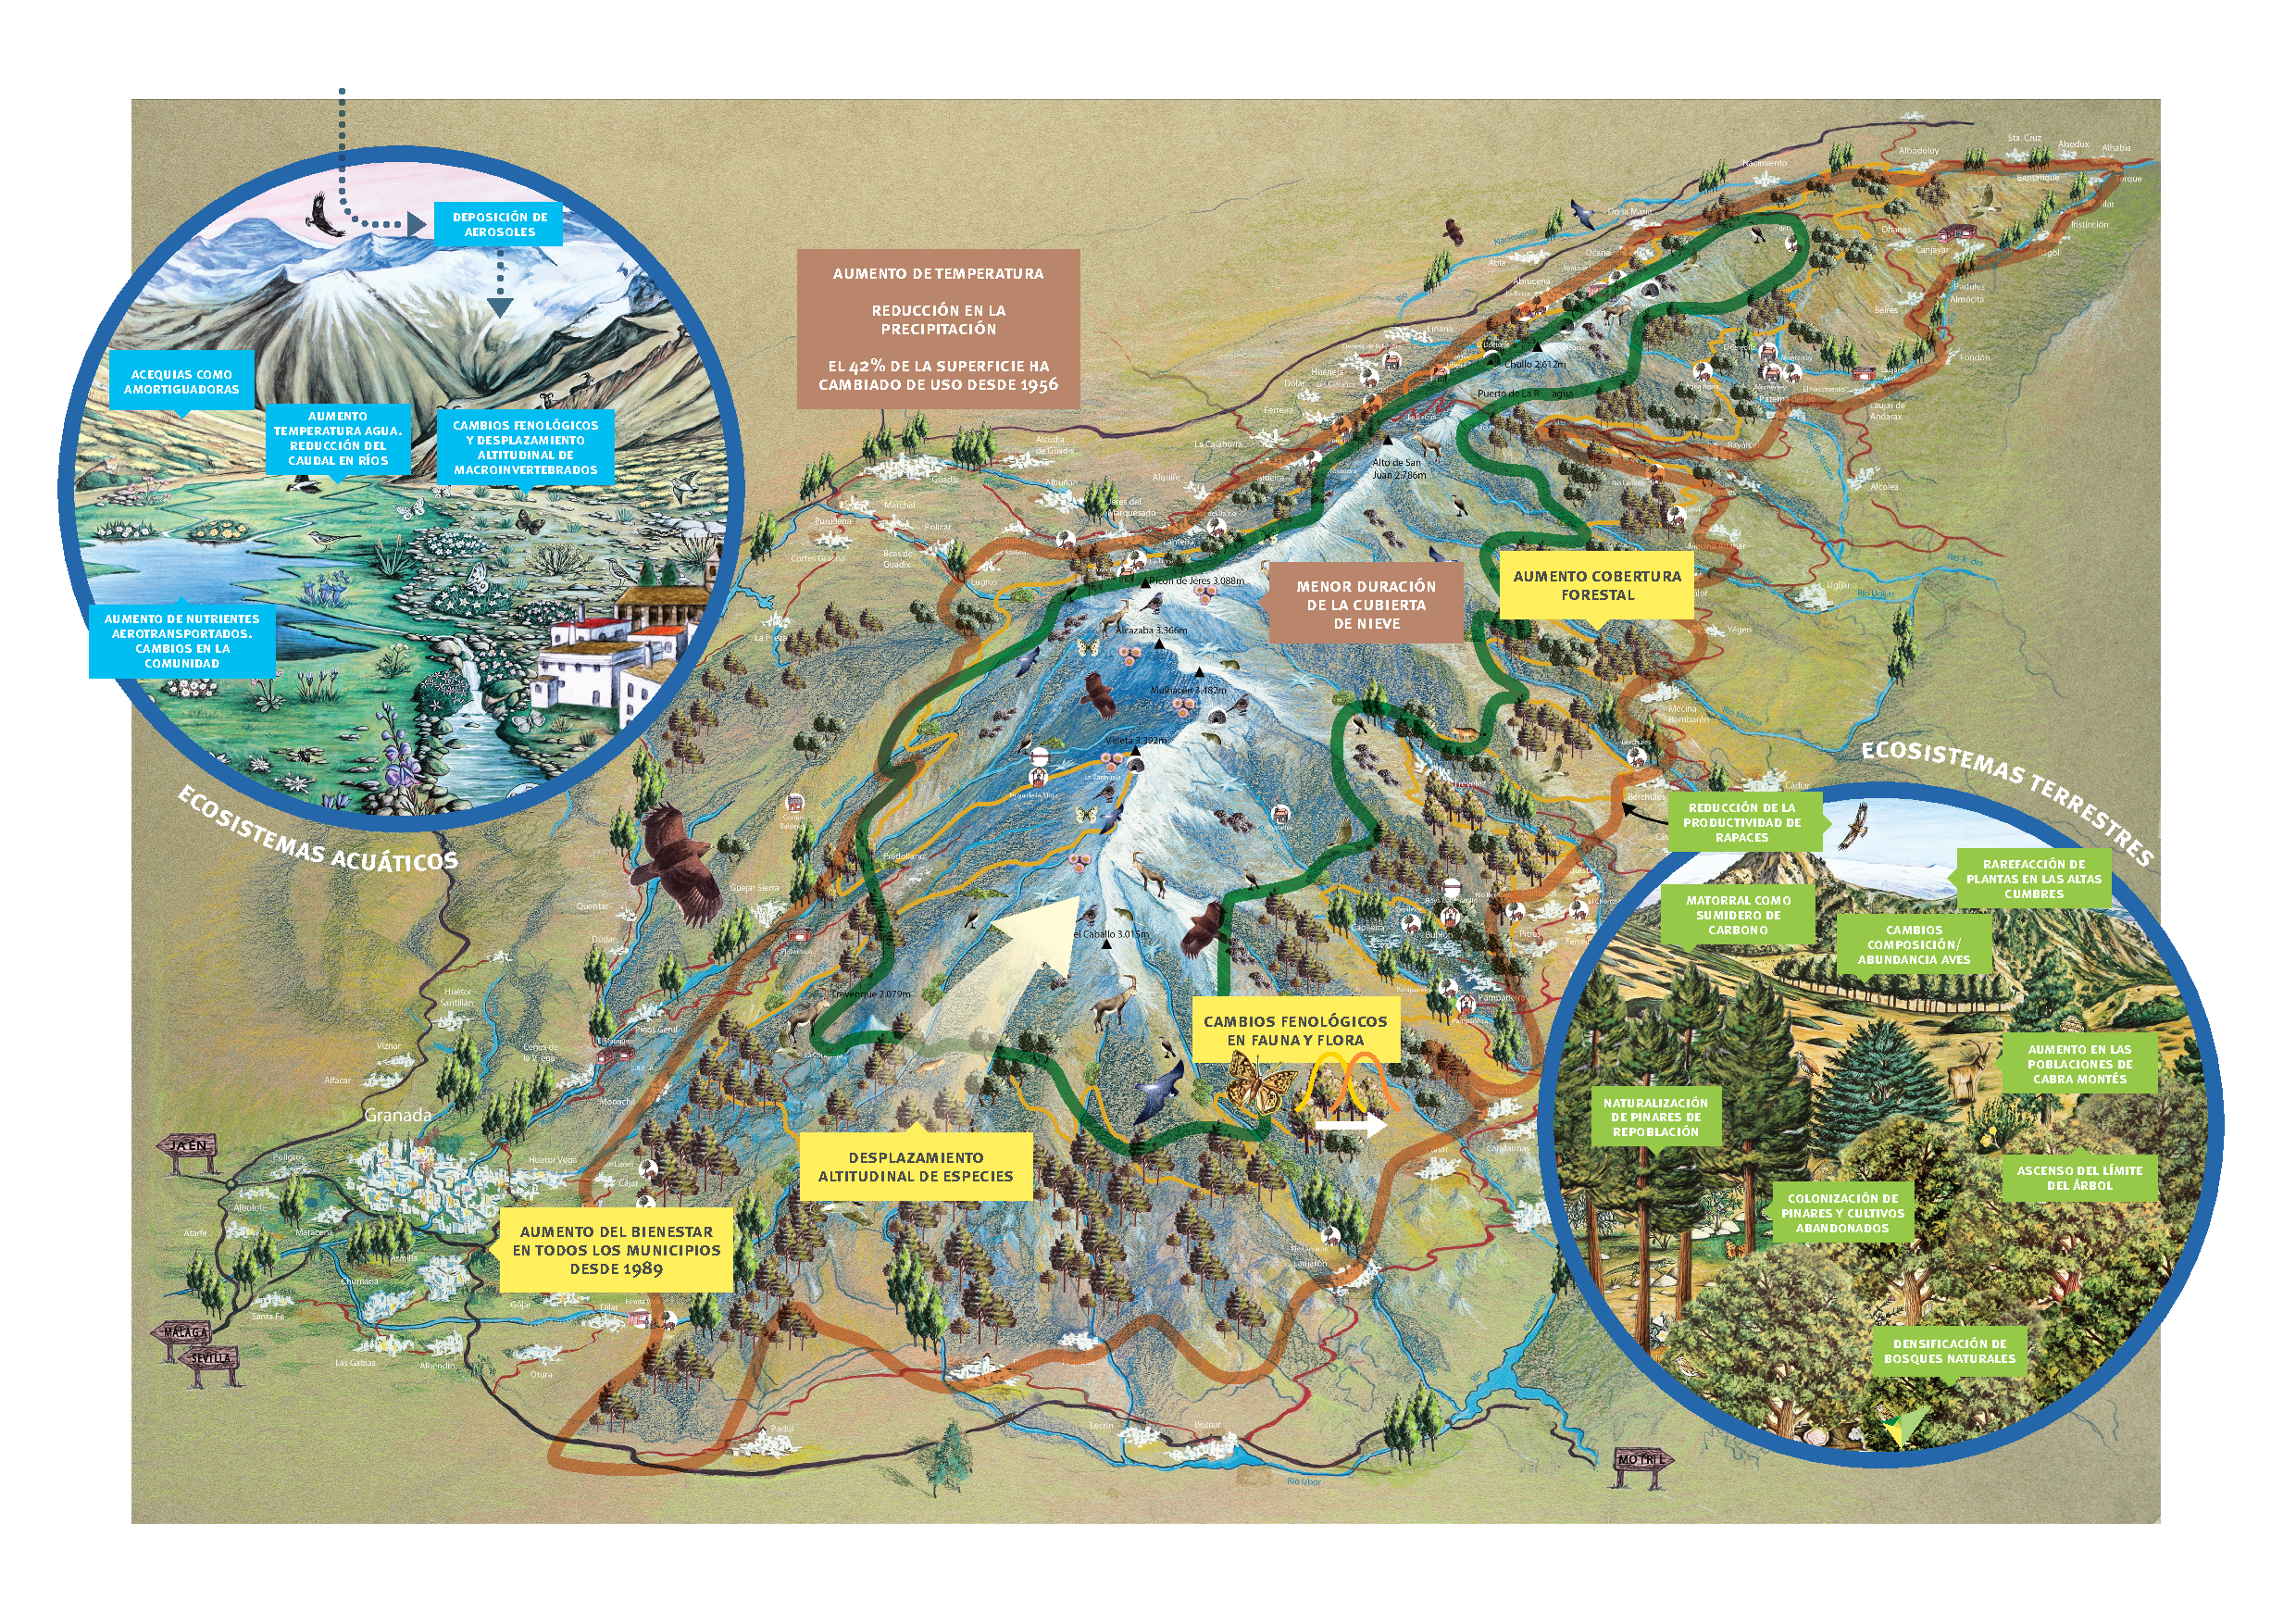
\includegraphics[width=\textwidth]{img/intro/intro-impacto-cambio-global.pdf} \caption{Principales impactos del cambio global en Sierra Nevada una región montañosa del sur de la Península Ibérica. Fuente: \citet{Zamoraetal2015HuellaCambio}.}\label{fig:intro:cambio-global}
\end{figure} 

\section{... y con cambio climático}\label{sec:intro:climate-change}

En la actualidad existen evidencias científicas de los efectos del cambio climático sobre los sistemas naturales \autocites{IPCC2013ClimateChange}. Muchos procesos se están viendo alterados debido al cambio climático: cambios en el área de distribución de las especies \autocites{Thuilleretal2005ClimateChange}; alteraciones fenológicas \autocites{GordoSanz2005PhenologyClimate, EstiartePenuelas2015AlterationPhenology}, invasiones de especies \autocite{GonzalezMorenoetal2014PlantInvasions}, aumento en la severidad e incidencia de plagas forestales \autocites{Hodaretal2012CambioClimatico,HodarZamora2004HerbivoryClimatic}, alteraciones en las interacciones ecológicas \autocites{MontoyaRaffaelli2010ClimateChange}, por citar algunos. Estos y otros cambios están modificando la composición, estructura y el funcionamiento de los ecosistemas, así como los bienes y servicios que éstos proporcionan \autocites{Dingetal2016ValuingClimate}. Para la región Mediterránea, los efectos del cambio climático se espera que sean más severos que en otras regiones de la Tierra \autocites{Giorgi2006ClimateChange,IPCC2013ClimateChange} y en los ecosistemas forestales mediterráneos estos cambios tendrán impactos significativos \autocites{Regato2008AdaptingGlobal,RescodeDiosetal2006ClimateChange,Penuelasetal2017ImpactsGlobal,HerreroZavala2015BosquesBiodiversidad}.  

En la región Mediterránea se ha registrado en las últimas décadas un aumento generalizado de las temperaturas, así como un cambio en los patrones de precipitación \autocites{PerezBoscolo2010ClimateSpain,GiorgiLionello2008ClimateChange,Crameretal2020ClimateEnvironmental}. Para Sierra Nevada, usando datos datos de estaciones meteorológicas y mapas climáticos de alta resolución \autocites{Benitoetal2014ClimateSimulations}, también se han encontrado tendencias positivas para la temperaturas mínimas y máximas anuales, así como un patrón generalizado de reducción de la precipitación anual desde la década de 1960 \autocites{PerezLuqueetal2016SenalesCambio,PerezLuqueetal2021ClimaNevadaBase}.  

Una de las característica del cambio climático, además del aumento en las temperaturas y el cambio en el régimen de precipitaciones, es el aumento de los eventos extremos, tales como sequías, tormentas, inundaciones, etc. \autocite{IPCC2013ClimateChange}. A pesar de que la sequía es una característica del clima mediterráneo \autocites{Lionello2012}, en las últimas décadas se ha registrado un incremento en la duración, frecuencia y severidad de los eventos de sequía \autocites{LloydHughesSaunders2002DroughtClimatology, Sousaetal2011TrendsExtremes,Colletal2017DroughtVariability}, particularmente en el sur de Europa \autocites{VicenteSerranoetal2014EvidenceIncreasing,Staggeetal2017ObservedDrought,Spinonietal2015EuropeanDrought,Pascoaetal2017DroughtTrends}, donde además se ha observado una tendencia hacia veranos más secos \autocites{Spinonietal2017PanEuropeanSeasonal} (\figreft{fig:intro:sequia}). Este hecho cobra especial relevancia para el área Mediterránea, considerada una de las más vulnerables frente al cambio climático \autocites{Giorgi2006ClimateChange}, ya que las proyecciones a futuro pronostican un aumento de la severidad de los eventos climáticos extremos extremos \autocites{Hoerlingetal2012IncreasedFrequency,IPCC2013ClimateChange,Trenberthetal2014GlobalWarming,Spinonietal2018WillDrought}.  

\begin{figure}
	\centering
	\includegraphics[width=\textwidth]{img/intro/intro-sequia.pdf} \caption{Evolución temporal de la precipitación acumulada (año hidrológico) durante el periodo 1950-2020 para Sierra Nevada (datos procedentes de 28 estaciones meteorológicas). Los puntos representan la media y las barras de error, el error estándar. La línea negra indica la precipitación acumulada media para todo el periodo (585 mm). Las líneas rojas representan -1 y -2 desviaciones estándar (líneas punteadas y discontinuas respectivamente). Las líneas azules representan +1 y +2 desviaciones estándar (líneas punteadas y discontinuas, respectivamente). Datos de \autocite{PerezLuqueetal2021ClimaNevadaBase}}\label{fig:intro:sequia}
\end{figure}

El incremento en la frecuencia y severidad de las sequías está alterando el funcionamiento de los ecosistemas mediterráneos a diferentes escalas \autocites{Penuelasetal2017ImpactsGlobal,Forneretal2018ExtremeDroughts,Liuetal2020EffectsDecadal,OgayaPenuelas2021ClimateChange}, puesto que la sequía afecta a aspectos fisiológicos, funcionales, estructurales y demográficos de los ecosistemas forestales \autocites{Allenetal2010GlobalOverview, Assaletal2016SpatialTemporal}. No obstante, se están observando respuestas diferenciales de los ecosistemas forestales a la sequía \autocites{Andereggetal2020DivergentForest}, poniendo de manifiesto la importancia de otros aspectos como el momento en el que ocurre la sequía \autocites{Huangetal2018DroughtTiming}. Esto es de especial relevancia para especies de frondosas como el \Qpy que presenta una fenología de crecimiento bien marcada \autocites{PerezdeLisetal2016ChangesSpring}. 

\Qp presenta una alta vulnerabilidad al cambio climático en la Península Ibérica \autocites{GarciaValdesetal2013ChasingMoving,BenitoGarzonetal2008EffectsClimate,Benitoetal2011SimulatingPotential}, lo cual es particularmente importante en las zonas más cálidas de su distribución \autocites{GeaIzquierdoCanellas2014LocalClimate}. Las simulaciones basadas en modelos de distribución de especies pronostican un potencial desplazamiento del área de distribución, así como una disminución en la idoneidad del hábitat para esta especie \autocites{Mateoetal2010EffectsNumber,BenitoGarzonetal2008EffectsClimate,Felicisimo2011ImpactosVulnerabilidad,Felicisimoetal2012VulnerabilidadFlora,RuizLabourdetteetal2011ForestComposition,Urbietaetal2011MediterraneanPine,Benitoetal2011SimulatingPotential}, que potencialmente puede suponer una reducción en la superficie ocupada a consecuencia del aumento de temperatura pronosticado \autocites{BenitoGarzonetal2008EffectsClimate,Benitoetal2011SimulatingPotential}. Esto es particularmente importante para Sierra Nevada, donde además de la disminución del área de ocupación se prevé una migración altitudinal \autocites{Benitoetal2011SimulatingPotential,Benito2009EcoinformaticaAplicada}, así como un aumento de la competencia con otras especies, ya que las zonas actualmente ocupadas por los robledales en Sierra Nevada serán óptimas para los encinares \autocites{Benitoetal2011SimulatingPotential}.

\section{... y con cambios de uso}\label{sec:intro:land-use}

A menudo se pasa por alto que la actividad humana constituye un impulsor de cambio tan poderoso o incluso más que los impulsores naturales (\emph{i.e.}, la variación natural del clima), en particular para las regiones con una larga historia de manejo, como la región Mediterránea \autocites{NavarroGonzalezetal2013WeightLanduse,DoblasMirandaetal2017ReviewCombination}. En estas zonas, la susceptibilidad y la respuesta de los ecosistemas al cambio climático están condicionadas por los legados del uso del suelo \autocites{Munteanuetal2015Legacies19th,Mausolfetal2018LegacyEffects}. Los legados del uso pasado, interactúan con las perturbaciones climáticas recientes causadas por el hombre y pueden confundir su interpretación \autocite{Fosteretal2003ImportanceLanduse}. Esto es importante ya que en la Península Ibérica se ha constatado que una cuarta parte de los bosques actuales crecen en antiguos terrenos agrícolas y de pastoreo abandonados después de la década de 1950 \autocite{VilaCabreraetal2017NewForests}. En consecuencia, la modificación antropogénica del hábitat y sus legados representan una dimensión crítica para las poblaciones situadas en su borde de distribución, ya que pueden intensificar, enmascarar o retrasar el declive poblacional impulsado por el clima en estas zonas \autocites{VilaCabreraJump2019GreaterGrowth,SanchezdeDiosetal2020FagusSylvatica}. 
\begin{figure}[H]
	\centering
	\includegraphics[width=\textwidth]{img/intro/intro-usos.pdf} \caption{Principales usos antrópicos del robledal. Pilas de leña para carboneo tradicional (1); quemas para la creación de áreas de pastoreo y cultivos (2); leñas para uso doméstico (3); pastoreo (4); y producción de bellotas (5). \autocite[Fuente: ][]{PerezLuqueetal2021ManualGestion}}\label{fig:intro:usos}
\end{figure}

Los robledales de \Qp, al igual que otras formaciones forestales, han sido objeto de intensas presiones de origen antrópico que han provocado la reducción de su área de distribución, así como la modificación en sus patrones florísticos y estructurales \autocites{Gavilanetal2000EffectsDisturbance,Gavilanetal2007ModellingCurrent,Tarregaetal2006ForestStructure}. Históricamente se han explotado en monte bajo para la obtención de leñas, carbón, taninos y producción de casca \autocite{RuizdelaTorre2006FloraMayor}. También se han llevado a cabo clareos para crear pastos con bajas densidades de árboles maduros que proporcionan bellotas, leñas y amplias áreas para el pastoreo; e incluso a veces se quemaban para crear áreas de pastoreo \autocite{ValbuenaCarabanaGil2017CentenaryCoppicing}. De hecho, el sobrepastoreo en estas formaciones provocaba unas importantes pérdidas de suelo, aspecto que se viene señalando por los gestores forestales desde final del siglo XIX \autocite{Laguna1872ComisionFlora}. Todos estos procesos antropogénicos han transformado tanto las estructuras de los robledales, que es difícil encontrar rodales que puedan considerarse como bosques naturales \autocite{RuizdelaTorre2006FloraMayor}. Esta presión antrópica también se ha observado en los robledales de Sierra Nevada \autocite{JimenezOlivencia1991PaisajesSierra}, donde el intenso aprovechamiento ganadero y forestal, la roturación de espacios para nuevos cultivos y pastos, la explotación de leña para uso doméstico o industrial, e incluso los incendios forestales, han ocasionado la reducción de la superficie que ocupaban estas formaciones \autocite{CamachoOlmedoetal2002AltaAlpujarra} (\figreft{fig:intro:usos}). Así, por ejemplo, el melojar de la Solana de la Dehesa de San Jerónimo, sufrió una tala masiva en la posguerra para utilizar la leña como gasógeno para los automóviles \autocite{Prieto1975BosquesSierra}. En algunas zonas de Sierra Nevada, la presión antrópica ha sido tan intensa, que se perdió por completo la cubierta forestal, ocasionando graves problemas de erosión \autocite{MesaGarrido2019ReforestacionSilvicultura,RomeroZurbano1909DivisionHidrologicoforestal}. Todas estas actuaciones condujeron a una sobreexplotación de los robledales cuya configuración actual en Sierra Nevada parece depender, al igual que otras formaciones vegetales, del uso del pasado \autocite{NavarroGonzalezetal2013WeightLanduse}. Sin embargo, a partir de la segunda mitad del siglo XX se produjo un abandono rural que produjo una disminución de la presión antrópica sobre los ecosistemas forestales. Es por ello que analizar la dinámica de los robledales frente a los cambios de uso del suelo resulta crucial dada la importancia que tiene el uso del pasado en la configuración actual de estos ecosistemas, más teniendo en cuenta que representan uno de los bordes mas meridionales de su distribución. 


\section{Problemas de conservación del robledal en el borde de su distribución}\label{sec:intro:problemas}

Las principales amenazas que sufren los melojares parecen estar relacionadas con las transformaciones productivas y de usos del suelo generadas por los intensos cambios socioeconómicos ocurridos durante las últimas décadas \autocites{Vericatetal2012GestionAdaptativa,PiqueVericat2015EvolutionPerspectives}. Este conjunto de efectos se ha convertido en el principal agente transformador de los melojares, que además pueden actuar de forma sinérgica con los impactos derivados del cambio climático. La sustitución de los robledales en el pasado por cultivos y pastos relegó al robledal a las laderas y pendientes más inclinadas \autocites{GarciaJimenez20099230Robledales,BlancoCastroetal2005BosquesIbericos,JimenezOlivenciaetal2015EvolucionUsos,Allue1997GestionRobledales}. El abandono de los usos forestales tradicionales ha provocado posteriormente una acumulación de biomasa en el monte que incrementa la vulnerabilidad y la sensibilidad de estas formaciones ante los incendios forestales \autocites{GarciaJimenez20099230Robledales,Allue1997GestionRobledales,Calvoetal1999PostfireSuccession}. Por otro lado, debido a la gran capacidad de recuperación que presenta esta especie frente a perturbaciones puntuales (como un incendio) \autocites{Calvoetal1999PostfireSuccession,Calvoetal2003RegenerationWildfire}, el riesgo de sufrir incendios recurrentes aumenta debido a la acumulación de altas densidades de biomasa aérea \autocites{Canellasetal2004GrowthResponse,Canellasetal2008SilvicultureCarbon}.

Otras amenazas específicas sobre los melojares están relacionadas con los problemas de regeneración y baja supervivencia de las plántulas. Tradicionalmente se ha asumido que los robledales, debido a su debilitado estado de salud, producen pocas bellotas. De hecho, se han aclarado las masas con el objetivo de reducir la competencia por los recursos y mejorar el estado de la masa \autocites{Canellasetal2004GrowthResponse,Aldeaetal2017ThinningEnhances,MorenoFernandezetal2020InfluenceClimate}, lo cual puede derivar en una mayor capacidad de reproducción y de producción de bellota \autocites{Bravoetal2008SelviculturaMontes}. Sin embargo, se ha visto en algunas especies congéneres que estos efectos se mantienen solo en el corto plazo \autocites{SanchezHumanesEspelta2011IncreasedDrought}, y que incluso pueden llegar a producir una disminución de la producción de bellota \autocites{Martiniketal2017EffectThinning}.

Los robledales, al igual que otras especies del género \emph{Quercus}, también sufren la incidencia de plagas forestales, entre las que destaca el complejo de lepidótperos defoliadores. Este complejo que alberga a mas de 50 especies de diferentes familias de lepidótperos \autocites{Soria1988RelacionLepidopteros,Soria1987LepidopterosDefoliadores}, debilita el estado de salud de las masas forestales, afectando también a la producción de bellota. En Sierra Nevada, se han detectado mas de 25 especies de este complejo defoliador (J.M. Muñoz \emph{com. pers.}), comportándose algunas como plagas en determinados años (\emph{e.g. Lymantria dispar, Tortrix viridiana}).  

La dispersión de las bellotas se realiza principalmente por parte del arrendajo (\emph{Garrulus glandarius}). En Sierra Nevada, se ha observado un descenso en la densidad de este córvido, pasando de 6.6 ind/10 ha en los años 80 a 1.25 ind/10 ha en la actualidad \autocites{ZamoraBareaAzcon2015LongTermChanges}. Las bellotas de roble melojo son consumidas por varias especies de vertebrados como el ratón de campo (\emph{Apodemus sylvaticus}), el jabalí (\emph{Sus scrofa}) o el ganado doméstico \autocites{Pereaetal2014InteraccionesPlantaanimal,Gomezetal2001ProblemasRegeneracion}, que actúan en diferentes microhábitats. Por ejemplo, los jabalís prefieren los espacios abiertos mientras que los ratones consumen selectivamente las bellotas situadas debajo de los arbustos, por lo que disminuyen los lugares seguros para el reclutamiento \autocite{Gomez2003ImpactVertebrate}. 

La sequía estival junto con los daños causados por los ungulados provocan una considerable mortalidad de plántulas y juveniles de esta especie \autocites{Pereaetal2014InteraccionesPlantaanimal,Barazaetal2004HerbivoryHas}. Las plántulas emergidas sufren unas altas tasas de mortalidad, debidas fundamentalmente al pisoteo y al consumo por parte de vertebrados como jabalíes, ratones y liebres \autocites{Pereaetal2014InteraccionesPlantaanimal,Gomez2003ImpactVertebrate}. Por otro lado, la herviboría también se ve condicionada por las diferencias en las características químicas de las plántulas de especies arbóreas, propiciando un consumo diferencial por parte de los ungulados \autocites{Baraza2005EfectoPequenos,Barazaetal2007InfluenciaCaracteristicas,Barazaetal2004HerbivoryHas}. En Sierra Nevada, el roble y el arce (\emph{Acer opalus} subsp. {granatensis}) presentan una alta calidad nutritiva en comparación con otras especies forestales con las que conviven (\emph{e.g} pino albar, pino salgareño y encina), lo que supone una alta probabilidad de consumo, incluso cuando son juveniles. Además, el efecto de la herbivoría sobre la regeneración del roble, y de otras especies forestales, depende, también de la frecuencia y severidad con la que son ramoneados los individuos (juveniles), y de la capacidad de tolerancia que presentan. Así los juveniles de las especies con mayor probabilidad de consumo (menos resistentes), muestran una mayor recuperación tras la herbivoría (tolerancia) respecto a las especies menos palatables \autocite{Barazaetal2007InfluenciaCaracteristicas}.   

Otro factor a tener muy en cuenta respecto al reclutamiento del robledal es la intensidad y duración de la sequía estival. Se ha comprobado que el roble junto con la encina son las especies que presentan mayor probabilidad de reclutamiento en veranos secos \autocites{Mendozaetal2009SeedingExperiment}. Asimismo, cuando ocurren veranos más húmedos, aumenta drásticamente la supervivencia del banco de plántulas de roble \autocites{Mendozaetal2009SeedingExperiment}. 

\subsection{Conservación de los robledales}\label{sec:intro:conservation}

\Qp está incluida con la categoría de \emph{"Preocupación menor"} en la Lista Roja de Especies Amenazadas de la IUCN \autocites{Goreneretal2017QuercusPyrenaica}, así como en la Lista Roja Europea de Árboles \autocites{Riversetal2019EuropeanRed}. En algunos catálogos autonómicos aparece con diferentes grados de protección. En Andalucía, se consideró como Vulnerable con riesgo menor pendiente de conservación \autocites{Viveroetal2000QuercusPyrenaica}. Asimismo se incluye en la Lista Roja de la Flora Vascular de Andalucía bajo la categoría \emph{"NT"} (Casi Amenazada) \autocites{Cabezudoetal2005ListaRoja}. Finalmente, en Sierra Nevada siguiendo criterios UICN se ha catalogado como de menor riesgo, dependiente de la conservación (LRcd) \autocites{Blancaetal1998ThreatenedVascular,Blancaetal2001VegetacionSierra, Lorite2016UpdatedChecklist, Loriteetal2007EstimationThreatened}. 

Los bosques de \Qp están protegidos a nivel europeo por la Directiva Hábitats (92/43/CEE) (en el anexo I como \emph{"9230 Robledales galaico-portugueses con Quercus robur y Quercus pyrenaica"}) e incluidos en la Red Natura 2000. Aparecen en diferentes esquemas de clasificación de hábitats:

\begin{itemize}
\item EUNIS Hábitat Classification \autocites{Daviesetal2004EUNISHabitat}: G1.7B4 Baetic [\Qpy] forests
\item Paleartic Habitat Classification 1996 \autocite{DevillersDevillersTerschuren1998ClassificationPalearctic}: 41.6 \Qpy forests 
\end{itemize}

El 18.41\% de la distribución actual de los melojares en España aparece bajo algún nivel de protección ya que se encuentran en diversos espacios naturales protegidos. Asimismo aparece en la Lista Patrón de Hábitats Terrestres como \emph{41.64 Bosques béticos de Quercus pyrenaica.}


\section{Conocimiento de la dinámica de los robledales en el borde de su distribución}\label{sec:intro:conocimiento}

Los robledales de Sierra Nevada han sido objeto de numerosos estudios, predominando los de índole ecológico y fitosociológico. Se han realizado trabajos de caracterización de los robledales desde un punto de vista fitosociológico, llevando a cabo clasificaciones basadas en la composición y abundancia de especies \autocites[\emph{e.g.}][]{MartinezParrasMoleroMesa1982EcologiaFitosociologia,Loriteetal2008PhytosociologicalReview, MelendoValle2000EstudioComparativo}. Asimismo, se ha abordado diferentes aspectos ecológicos, como por ejemplo (por citar algunos): efecto de la herbivoría en el reclutamiento \autocites[\emph{e.g.}][]{Gomez2003ImpactVertebrate,Barazaetal2004HerbivoryHas,Barazaetal2007InfluenciaCaracteristicas}; el reclutamiento bajo diferentes escenarios de sequía \autocites{Mendozaetal2009SeedingExperiment}; la evaluación de las respuestas de los juveniles a diferentes escenarios lumínicos \autocite{GomezAparicioetal2008OakSeedling}; la evaluación de la supervivencia de juveniles por encima del límite del árbol \autocites{Leverkusetal2015RestoringPresent}. Por otro lado también se han abordado estudios genéticos de los diferentes tipos de robledales \autocites[\emph{e.g.}][]{ValbuenaCarabanaGil2011EvaluacionEstructura,ValbuenaCarabanaGil2013GeneticResilience,ValbuenaCarabanaGil2017CentenaryCoppicing}, así como estudios de la microbiota de estas formaciones \autocites{CoboDiazetal2017TaxonomicFunctional,Lasaetal2019BacteriaEndosphere, Lasaetal2019MetabarcodingReveals}. Otros trabajos han evaluado el funcionamieno de estas formaciones usando indices derivados de teledetección \autocites{Dionisioetal2012SatelliteBasedMonitoring,AlcarazSeguraetal2015CambiosProductividad,RequenaMulloretal2018AssessmentEcosystem}, así como las tendencias de crecimiemto usando metodos dendrocronológicos  \autocites{GeaIzquierdoCanellas2014LocalClimate,RubioCuadradoetal2018AbioticFactors}. Destacán también los estudios de cambio de uso \autocite{JimenezOlivenciaetal2015EvolucionUsos,CamachoOlmedoetal2002DinamicaEvolutiva}, y aquellos donde se propone la utilización de plantas nodrizas para la restauración de robledales \autocites{Castroetal2006RestoringQuercus,GomezAparicioetal2004ApplyingPlant}. 
Éstos y otros estudios, han aportado una valiosa información sobre aspectos concretos de la ecología y el funcionamiento de los robledales. No obstante, en este memoria doctoral, pretendemos aumentar ese conocimiento centrándonos en varios aspectos relacionados con la dinámica de funcionamiento de esta formación frente al cambio global (cambios de uso y cambio climático) en el límite sur de su distribución.    

\section{Objetivos}\label{sec:intro:objetivos}
Así pues el \textbf{objetivo} general de esta memoria doctoral es analizar la dinámica de funcionamiento frente al cambio global de los robledales de \Qp situados en Sierra Nevada, una región montañosa que representa uno de los límites geográficos de su distribución, donde estas formaciones han sido objeto de intensas presiones antrópicas. 

Los objetivos específicos son: 

\paragraph{\emph{Caracterizar los robledales de Sierra Nevada desde un punto de vista ambiental}}\mbox{} \\
Bajo la hipótesis de que las poblaciones del limite sur de distribucion geográfica de \Qp localizadas en zonas de montaña son representativas de diferentes condiciones ambientales a escala local debido a los fuertes gradientes topográficos existentes, queremos analizar si las poblaciones de robledal de Sierra Nevada habitan en condidiones similares, y hasta qué punto la variabilidad ambiental se corresponde con diversidad florística. En este sentido, pretendemos: \emph{(i)} determinar las variables ambientales que mejor explican la distribución de las poblaciones de melojo en Sierra Nevada; \emph{(ii)} identificar grupos de poblaciones de robledal en función de la composición florística y las condiciones ambientales; y \emph{(iii)} analizar si la agrupación de las poblaciones de melojo en función de las variables ambientales coincide con su agrupación en función de la composición florística.

\paragraph{\emph{Analizar el proceso de colonización de hábitats degradados próximos a las masas de robledal en Sierra Nevada}}\mbox{} \\
Tras el abandono de actividades tradicionales, queremos analizar el proceso de colonización de hábitats degradados (campos de cultivo abandonados) próximos a los robledales y explorar si existen diferencias entre las poblaciones en el límite sur de su distribución. 

\paragraph{\emph{Cuantificar el papel de los robledales de Sierra Nevada como sumidero de carbono y analizar su tendencia temporal}} \mbox{} \\
El secuestro de carbono es uno de los servicios ecosistémicos más relevantes que proporcionan los bosques mediterráneos, siendo un indicador de la capacidad del ecosistema para contribuir a la regulación del clima. Los robledales, como ecosistemas mediterráneos representan un sumidero de carbono. El objetivo de este capítulo es cuantificar la capacidad  de secuestro de carbono de los robledales de Sierra Nevada, situados en el borde de su distribución, explorando las posibles diferencias entre las poblaciones de robledal dentro de esta región montañosa. Asimismo estamos interesados en analizar la evolución temporal de este servicio ecosistémico 

\paragraph{\emph{Analizar los efectos del cambio climático en la productividad de los robledales en Sierra Nevada}} \mbox{} \\
Pretendemos evaluar como las alteraciones en los patrones de disponibilidad hídrica debido al cambio climático pueden afectar a la productividad de esta formación forestal. Sabemos que los robledales presentan una estación de crecimiento bien definida y centrada en la estación estival. Por ello es de interés evaluar la productividad de los robledales (utilizando índices de vegetación obtenidos a partir de imágenes de satélite) frente a cambios en los patrones de disponibilidad hídrica. Nos centraremos en analizar modificaciones en la cantidad de agua (disminución de la disponibilidad de agua debido a eventos de sequía) así como alteraciones en la distribución temporal de la disponibilidad de agua (\emph{p.ej.}: adelantos en la fusión de la cubierta de nieve).

\paragraph{\emph{Evaluar la resiliencia de los robledales en su borde de distribución frente a eventos de sequía}}\mbox{} \\
El cambio global supone un reto para los ecosistemas forestales localizados en el borde de su distribución debido a su vulnerabilidad a los eventos de sequía. Nuestro objetivo es analizar la resiliencia a varios eventos de sequía de las poblaciones relíctas de \Qp situadas en Sierra Nevada. Para ello, combinaremos información de teledetección y métodos dendroecológicos para evaluar el impacto de la sequía tanto en el verdor de la vegetación (como indicador del crecimiento primario) como en el crecimiento radial de los árboles (como indicador del crecimiento secundario).

\paragraph{Identificar y cuantificar los servicios ecosistémicos proporcionados por los robledales en Sierra Nevada}\mbox{} \\
Realizaremos una revisión de los principales servicios ecosistémicos proporcionados por los robledales combinando revisiones bibliográficas con conocimiento experto y datos de Sierra Nevada, con el objetivo de poner de relieve los diferentes servicios ecosistémicos que proporcionan estas formaciones para incorporarlas a las estrategias de gestiòn de estos ecosistemas. 

   
% !TEX root = ../my-thesis.tex
%
\selectlanguage{spanish} 
\chapter{Metodología general}
\label{sec:metodologia}

\section{El roble melojo}
\label{sec:metodologia:qp}

\Qpw es un árbol caducifolio de hojas marcescentes que alcanza hasta 20-25 m, de copa amplia (\figref{fig:metodologia:features-qp}). La corteza es cenicienta o pardo-grisácea, gruesa y agrietada. El tronco aparece muchas veces tortuoso. Ramillas pardas cuando jóvenes, después grisáceas, tomentosas. Presenta un sistema radical muy potente con numerosas raíces horizontales, superficiales, copiosamente estoloníferas, que dan lugar a la formación de matas periféricas tapizantes. Hojas pinnatífidas o pinnatipartidas, de base truncada o cordada; las adultas de haz verde y glabrescente y envés densamente tomentoso, con los pelos estrellados, que a menudo se mantienen marchitas y sin caer durante gran parte del invierno. Flores unisexuales; las masculinas en amentos laxos, colgantes, con perianto de lóbulos hirsutos y estambres expertos; las femeninas con estilos en el interior de un involucro de numerosas escamas (cúpula), en grupos raciformes de 1 a 4, sentadas o cortamente pedunculadas. Fruto en aquenio (bellota), envuelto por la cúpula en su parte basal, solitario o en grupos de 2-3, de color pardo-amarillento. Florece en abril y mayo; las bellotas maduran en noviembre y diciembre del mismo año.

\begin{figure}
	\centering
	\includegraphics[width=\textwidth]{img/metodologia/metodologia-features-qp.png} \caption{Características del roble melojo (\Qpw). Fotos: M. Iglesias (raíces); A.J. Pérez-Luque.} \label{fig:metodologia:features-qp}
\end{figure}

Los robledales de roble melojo o melojares son formaciones dominadas por \Qpw que se distribuyen desde el suroeste de Francia hasta el noreste de Marruecos, ocupando su mayor extensión en la Península Ibérica, donde abarcan una amplia variedad de sitios y nichos ecológicos (\figref{fig:metodologia:distroble}) \autocites{NietoQuintanoetal2016QuercusPyrenaica, GarciaJimenez20099230Robledales,VilchesdelaSerna2014ComprehensiveStudy,delaSernaetal2016MarcescentQuercus}. Según el Inventario Forestal Nacional \autocite{Villanueva2005TercerInventario}, estas formaciones ocupan 845 511 ha, lo que supone aproximadamente el 5\% de la superficie forestal de España. 

\begin{figure}[h]
	\centering
	\includegraphics[width=0.75\textwidth]{img/metodologia/metodologia-robledal-spain-v2.pdf} \caption{Distribución de los bosques de \Qpy en la Península Ibérica. Elaboración propia a partir del Mapa Forestal Español} \label{fig:metodologia:distroble}
\end{figure}


 Esta especie requiere de un mínimo de humedad estival para sobrevivir, que algunos autores han estimado en al menos 100 mm de precipitación entre mayo y agosto \autocite{BlancoCastroetal2005BosquesIbericos, Prieto1975BosquesSierra}. En Sierra Nevada el aporte extra de humedad necesario proviene de dos vías: de los ríos y acequias de careo, o del aire húmedo proveniente del Mediterráneo \autocites{PrietoEspinosa1977AestisilvaSierra, MartinezParrasMoleroMesa1982EcologiaFitosociologia,PerezRayaetal1990VegetacionSierra}. En efecto, los melojares en Sierra Nevada aparecen en aquellos enclaves más húmedos y de menor índice de insolación, principalmente barrancos y fondos de valle donde se dan unas condiciones microclimáticas favorables, tal y como ocurre en la zona occidental en orientaciones norte (ríos Alhama de Lugros, Maitena, Vadillo, Genil, Monachil, Dílar y Dúrcal) (\figref{fig:metodologia:disposicion}a); o situados ocupando una determinada altura en la vertiente sur (Alpujarras: loma de Cáñar, barranco del Poqueira, loma de Pitres-Busquístar) en donde actúan como una banda de vegetación que intercepta la humedad procedente del Mediterráneo \autocites{Lorite2001VegetacionSierra,PrietoEspinosa1977AestisilvaSierra} (\figref{fig:metodologia:disposicion}b). Estas diferencias también tienen reflejo en la composición florística de las poblaciones de ambas vertientes \autocites{Loriteetal2008PhytosociologicalReview,MelendoValle2000EstudioComparativo}.  

\begin{figure}
	\centering
	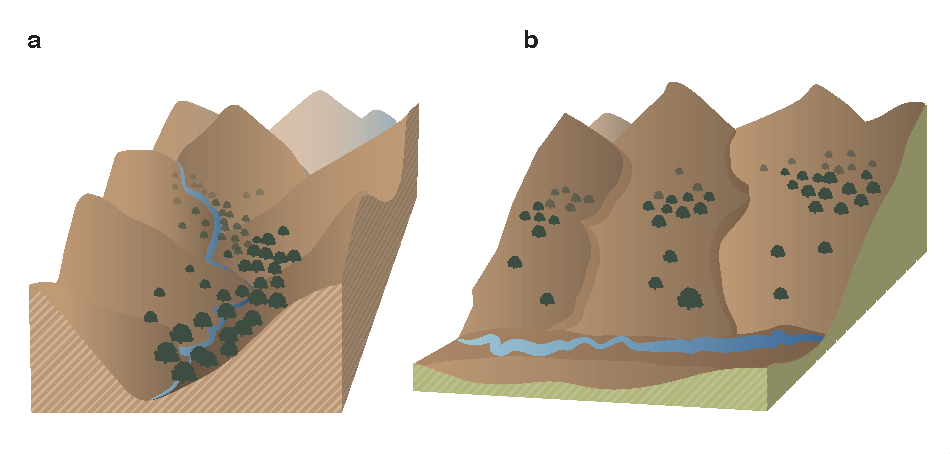
\includegraphics[width=\textwidth]{img/metodologia/metodologia-disposicionSN.pdf}\caption{Disposición de las poblaciones de robledal en la cara norte (\emph{e.g.} Robledal del valle del Río Genil)(\textbf{a}) y sur (\emph{e.g.} Robledal de Cáñar)(\textbf{b}) de Sierra Nevada. Modificado a partir de \citet{PrietoEspinosa1977AestisilvaSierra}.} \label{fig:metodologia:disposicion}
\end{figure}

\section{Área de estudio}
\label{sec:metodologia:sn}

Sierra Nevada es una región montañosa situada en el sur de Europa, que ocupa mas de 2 000 km\textsuperscript{2} (\figref{fig:metodologia:mapa-sn}). Presenta un rango altitudinal que varía entre 860 y 3 482 \elev, incluyendo la cumbre más alta de la Península Ibérica (Mulhacén). El clima es mediterráneo, caracterizado por inviernos fríos y veranos calurosos, con una pronunciada sequía estival. La temperatura media anual desciende en altitud desde los 12-16ºC por debajo de los 1 500 \elev hasta los 0ºC por encima de los 3 000 \elev de altitud. La precipitación media anual es muy irregular, con valores que oscilan entre los 250 y los 700 mm anuales, dependiendo  principalmente de la altitud y de la compleja orografía \autocites{PeinoCalero2020AnalisisVariabilidad, PerezLuqueetal2021ClimaNevadaBase}. Las precipitaciones invernales son principalmente en forma de nieve por encima de los 2 000 \elev de altitud \autocite{PerezPalazonetal2015ExtremeValues}. Geológicamente, la zona central está compuesta por rocas silíceas, principalmente micaesquistos, rodeadas de calizas y dolomías \autocite{RodriguezFernandez2017ParqueNacional}. Esta región montañosa alberga un total de 2 353 taxones de plantas vasculares, representando el 33\% y el 20\% de la flora de España y de Europa respectivamente \autocite{Lorite2016UpdatedChecklist}. Además presenta una alta tasa de endemicidad con 95 taxones vegetales endémicos \autocites{Loriteetal2007EstimationThreatened,Loriteetal2020FloraSNevadaTrait}. La cubierta forestal de Sierra Nevada está dominada por plantaciones de pino (\emph{Pinus halepensis} Mill., \emph{P. pinaster} Ait., \emph{P. nigra} Arnold subsp. \emph{salzmannii} (Dunal) Franco, y \emph{P. sylvestris} L.) que cubren aproximadamente 37 000 ha. Los bosques autóctonos están dominados principalmente por la encina (\emph{Quercus ilex} subsp. \emph{ballota} (Desf.) Samp.) ocupando zonas de baja y media montaña (11 000 ha) y el roble melojo (\Qpw) que va desde los 1 100 a los 2 000 \elev, cubriendo unas 3 400 ha \autocites{Lorite2001VegetacionSierra, PerezLuqueetal2019MapEcosystems}.

\begin{figure}
	\centering
	\includegraphics[width=0.99\textwidth]{img/metodologia/metodologia-mapasn.jpg}
	\caption{Localización (\textbf{a}) y vista de satélite de Sierra Nevada (\textbf{b}). Distribución espacial de los ecosistemas de Sierra Nevada  (\textbf{c}). Se indican los pisos bioclimáticos. Imagen de la Estación Espacial Internacional tomada en diciembre de 2014; cortesía de \emph{Earth Science and Remote Sensing Unit, NASA Johnson Space Center}.}\label{fig:metodologia:mapa-sn}
\end{figure}


Sierra Nevada contiene 27 hábitats tipo incluidos en la Directiva Hábitats, 28 especies de aves del Anexo I de la Directiva Aves y 15 especies de animales incluidas en el Anexo II de la Directiva Hábitats (1 reptil, 2 anfibios, 7 mamíferos y 5 invertebrados). Todo ello hace que esté considerada como uno de los \emph{hotspots} de biodiversidad más importantes en la Región Mediterránea \autocites{Blanca1996ProteccionFlora,Blancaetal1998ThreatenedVascular,MedailQuezel1999BiodiversityHotspots,Canadasetal2014HotspotsHotspots}. En Sierra Nevada hay 61 municipios con mas de 90 000 habitantes, siendo sus principales actividades económicas la agricultura, el turismo, la ganadería, la apicultura, la minería, y el esquí \autocite{FernandezMarquezSalinas2009ImpactoSocioeconomico}. El alto valor de biodiversidad y geodiversidad, así como su riquerza paisajística y cultural han hecho que Sierra Nevada presente varios reconocimientos y cuente con diversas figuras legales de protección. Además de contar con un Parque Nacional y un Parque Natural, Sierra Nevada es una Reserva de la Biosfera (MaB, Unesco). Está incluida en la red Natura 2000 como Zona de Especial Protección para las Aves y Lugar de Interes Comunitario (LIC). 

Una de las características más importantes de Sierra Nevada es la existencia de marcados gradientes altitudinales, ecológicos y climáticos \autocite{Zamoraetal2021UniendoMacro}. Así por ejemplo, existe un fuerte contraste climático entre las laderas soleadas y secas orientadas al sur, y las laderas sombreadas y más húmedas orientadas al norte. La heterogeneidad climática y topográfica existente en Sierra Nevada ofrece una gran diversidad de microhábitats, lo que ha permitido a esta región montañosa actuar como refugio de diferentes especies \autocites{MedailDiadema2009GlacialRefugia,GomezLunt2007RefugiaRefugia,BlancoPastoretal2019TopographyExplains}, incluyendo especies caducifolias de \emph{Quercus} durante la última glaciación \autocites{Olaldeetal2002WhiteOaks,RodriguezSanchezetal2010TreeRange,Petitetal2002IdentificationRefugia}. 

La existencia de estos gradientes confiere a Sierra Nevada, y a las regiones montañosas en general, el carácter de un excepcional laboratorio natural de seguimiento del cambio global \autocite{Zamora2010AreasProtegidas,Zamoraetal2017MonitoringGlobal}. De hecho, en 2008 se estableció el Observatorio de Cambio Global de Sierra Nevada (OBSNEV) (https://obsnev.es), un programa de seguimiento a largo plazo para evaluar el impacto del cambio global en los ecosistemas nevadenses \autocites{Aspizuaetal2010ObservatorioCambio,BonetGarciaetal2011SierraNevada}. Esta iniciativa está recopilando información útil y relevante sobre los efectos del cambio global en los sistemas socieoecológicos de Sierra Nevada \autocites{Zamoraetal2015HuellaCambio,Zamoraetal2017GlobalChange,PerezLuqueetal2016SenalesCambio, RamosLosadaetal2017TenYears}. Asimismo, y relacionado con la temática de la presente memoria doctoral, dentro de las metodologías de seguimiento de esta iniciativa, se vienen realizando diferentes análisis sobre los efectos del cambio global en las masas de robledal \autocites[ver por ejemplo][]{BonetGarciaetal2015ImpactosCambio,Aspizuaetal2012EvaluacionGestion,Munoz2012BosquesAutoctonos}. 

\subsection{Melojares en Sierra Nevada}
\label{sec:metodologia:qpsn}

En Sierra Nevada, los melojares ocupan actualmente una extensión de 3 400 ha \autocite{PerezLuqueetal2019MapEcosystems}, distribuidas entre los 1 000 y 2 000 \elev, y situados exclusivamente sobre suelos silíceos. 
Aunque representan menos del 7\% de la superficie forestal existente en Sierra
Nevada (\figref{fig:metodologia:mapa-sn}c), tienen una alta singularidad ecológica, presentando una alta diversidad de especies vegetales en comparación con las otras formaciones forestales \autocite{GomezAparicioetal2009ArePine,PerezLuqueetal2014SinfonevadaDataset},  y albergando diferentes especies vegetales consideradas relictas \autocite{Loriteetal2008PhytosociologicalReview, Blancaetal1998ThreatenedVascular} (Ver apéndice \ref{sec:appendix:multivar}). 

\section{Muestreos dendrocronológicos}
\label{sec:metodologia:dendro}

En el capítulo \ref{sec:dendro}, realizamos una estimación del crecimiento secundario de los robledales, para lo cual llevamos a cabo muestreos dendrocronológicos estándar para obtener series de crecimiento radial \autocite{Fritts1976TreeRings,CookKairukstis1990MethodsDendrochronology,Gutierrez2008DendrocronologiaMetodos,Natalinietal2017TecnicasHerramientas}.

En cada sitio de muestreo (Robledal del Genil, GEN; y Robledal de Cáñar, CAN; ver capítulo \ref{sec:dendro}), se seleccionaron entre 15 y 20 árboles de forma aleatoria. Para cada árbol focal (\emph{target tree}), se tomaron entre 2-3 testigos (\emph{cores}) de 5 mm de diámetro utilizando una barrena forestal o barrena de Pressler \autocite{GrissinoMayer2003ManualTutorial} (\figref{fig:metodologia:barrena-gente}). Los testigos se tomaron de forma perpendicular, y a una altura de 1.3 metros (Figura \figref{fig:metodologia:cores-combina}b). Cada testigo se etiquetó y se guardó en pajitas (preferiblemente de papel) para su transporte. Posteriormente en el laboratorio, los testigos se secaron al aire, y se montaron en soportes de madera para su posterior lijado y análisis (Figuras \figref{fig:metodologia:cores-combina}b-c). Durante el montaje, los testigos se colocaron de tal forma que las fibras quedaran perpendiculares a la superficie de lectura, y dejando visible la sección transversal, facilitando así la observación de los anillos \autocite{Fritts1976TreeRings,Natalinietal2017TecnicasHerramientas}. Para el lijado de las muestras se utilizó una lijadora eléctrica usando papeles de lija de granos sucesivamente mas finos (desde 60 hasta 1200).

\begin{figure}
    \centering
    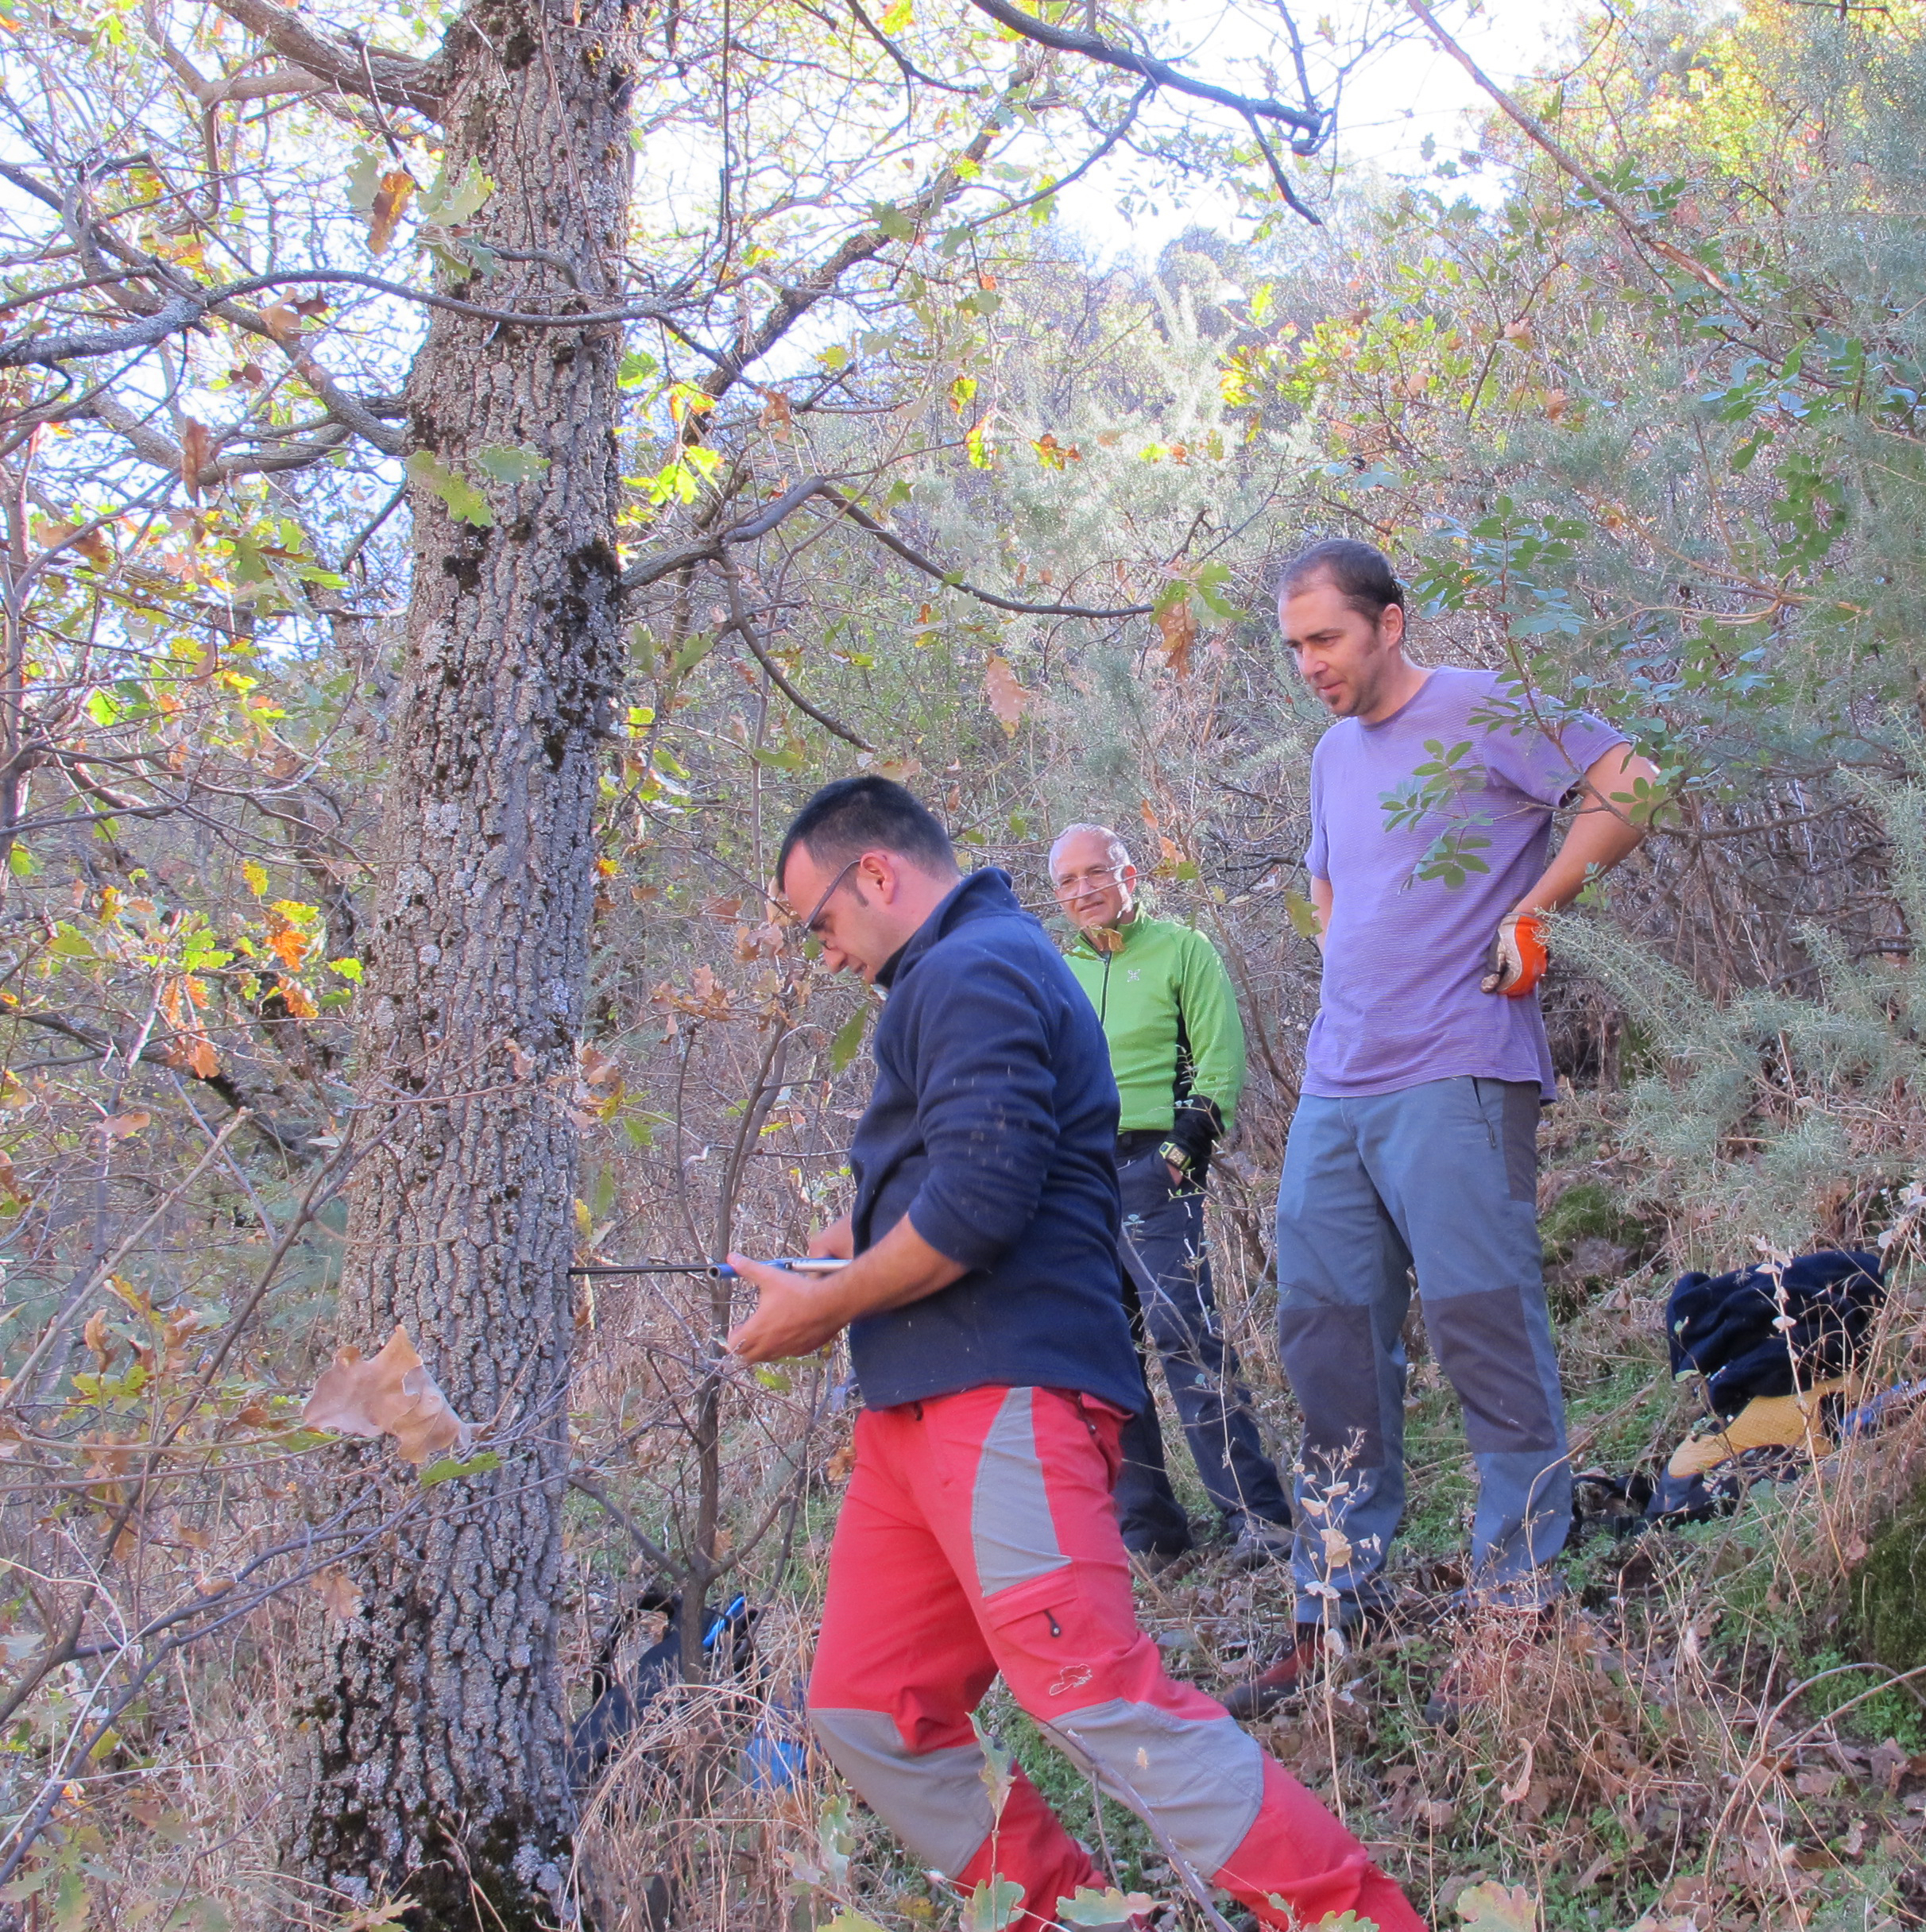
\includegraphics[width=0.8\textwidth]{img/metodologia/metodologia-barrena-gente.jpg}
    \caption{Obtención de testigos con Barrena de Pressler.}
    \label{fig:metodologia:barrena-gente}
\end{figure}

\begin{figure}
    \centering
    \includegraphics[width=0.99\textwidth]{img/metodologia/metodologia-cores-combina.jpg}
    \caption{Barrena de Pressler (\textbf{a}) obteniendo testigos de un ejemplar de \Qpy. Testigos montados sobre soporte de madera, antes (\textbf{b}) y después (\textbf{c}) de ser lijados.}
    \label{fig:metodologia:cores-combina}
\end{figure}



Posteriormente se procedió a la medición, desde la corteza hasta la médula, de la anchura de todos los anillos de crecimiento (\emph{RW}, \emph{ring width}) con una precisión de 0.01 mm, utilizando una mesa de medición LINTAB acoplada a un estereomicroscopio de alta resolución y a un ordenador con el software TSAP-Win (Rinntech, Heidelberg, Alemania). Una vez realizadas las mediciones, las series se sincronizaron visualmente y se dataron utilizando los estadísticos \emph{Gleichläufigkeit} (GLK), \emph{t-valor} e índice de datación cruzada (\emph{CDI}, \emph{crossdate index}) \autocite{Schweingruber1988TreeRings,BurasWilmking2015CorrectingCalculation}. Se sincronizaron los testigos pertenecientes al mismo árbol entre sí, construyeron cronologías de individuo, para posteriormente generar cronologías de sitio. La datación cruzada visual se verificó utilizando el programa COFECHA, que calcula la intercorrelación entre series mediante segmentos solapados \autocite{Holmes1983ComputerassistedQuality}. Este programa ayuda a evaluar la calidad de la datación cruzada y a identificar posibles problemas dentro de una serie de anillos de crecimiento \autocite{GrissinoMayer2001EvaluatingCrossdating}.

\subsection{Estimación de la competencia}
\label{sec:metodologia:competencia}
Para la estimación de la competencia de cada árbol focal (\emph{target tree}) se emplearon diferentes \textbf{índices de competencia}. La mayoría de los índices de competencia descritos en la literatura forestal pueden dividirse en dos grandes clases: los \emph{índices independientes de la distancia}, que utilizan únicamente información no espacial sobre el tamaño y el número de árboles agregados dentro de un área determinada (\emph{e.g.} una parcela o un rodal); y los \emph{índices dependientes de la distancia} que además incorporan las ubicaciones relativas de los árboles vecinos dentro del área \autocite{Contreras2011,GeaIzquierdoCanellas2009AnalysisHolm,BurkhartTome2012IndicesIndividualtree}. Los índices dependientes de la distancia, aunque son mas tediosos de obtener, presentan una mejor correlación con el crecimiento que los índices independientes de la distancia \autocites{GeaIzquierdoCanellas2009AnalysisHolm,Contreras2011,Maleki2015}. En nuestro caso empleamos los índices independientes de la distancia, \emph{densidad} ($n \; árboles \cdot ha^{-1}$) y \emph{área basal} ($m^{2} \cdot ha^{-1}$); así como el índice dependiente de la distancia \emph{ratio de tamaños proporcional a la distancia} (\emph{srd}, del inglés \emph{size ratio proportional to distance}) calculado como \[\mathrm{srd} = \sum_{i=1}^{n} ( \frac{dbh_j}{dbh_i}) \times \left[\frac{1}{(dist_{ij} + 1)} \right ]\]
siendo \(dbh_i\) y \(dbh_j\) los diámetros a la altura del pecho del árbol \(i\) y el árbol focal (\(j\)) respectivamente; y \(dist_{ij}\) la distancia entre ambos árboles.

Se muestrearon todos los árboles vivos con DBH \textgreater{} 7.5 cm dentro de una parcela circular de 10 m de radio, tomando como centro el árbol focal. Para cada árbol, se anotó la especie, se midió la altura y el DBH, así como la distancia y ángulo (\emph{azimuth}) respecto al árbol focal (\figref{fig:metodologia:competence}).


\begin{figure}
	\centering
	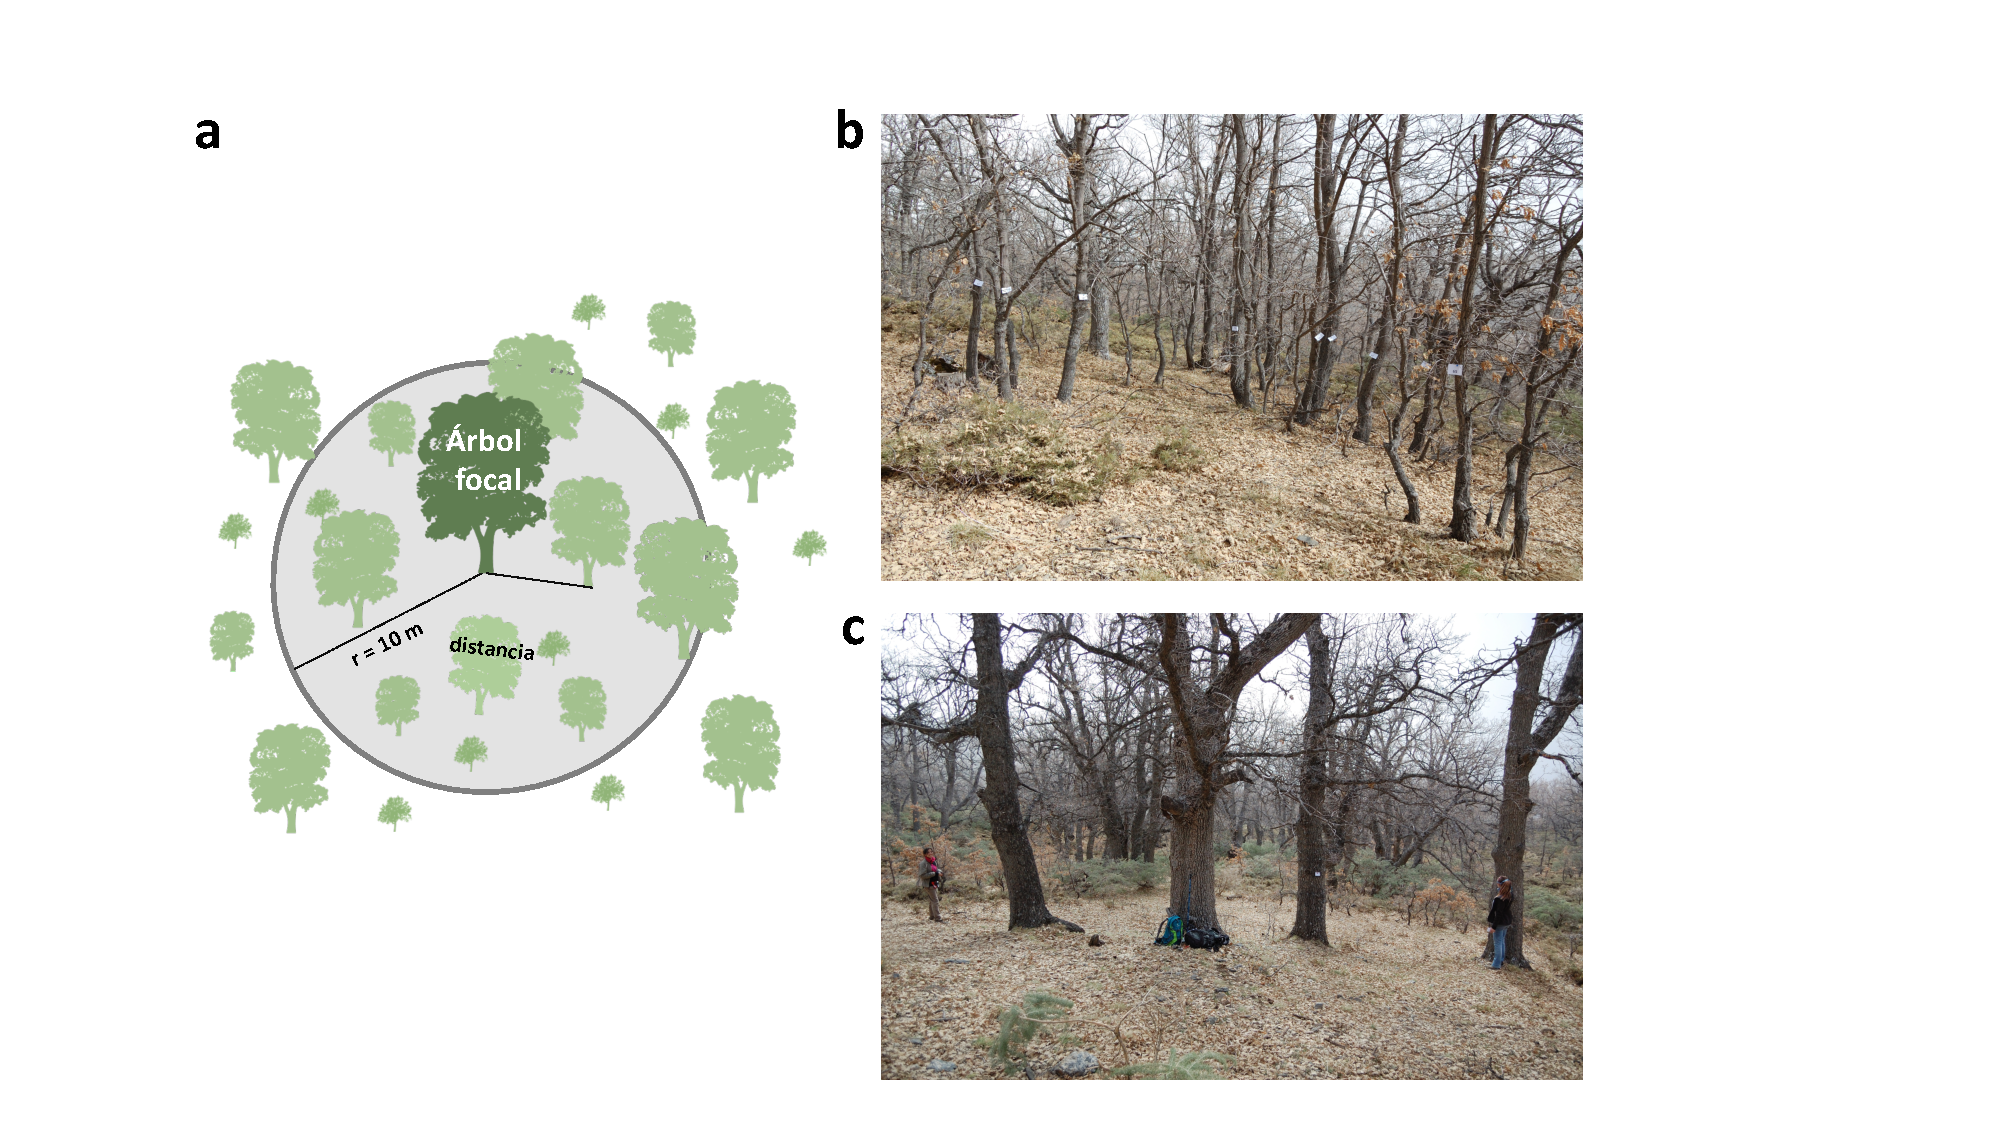
\includegraphics[width=0.99\textwidth]{img/metodologia/metodologia-competence.pdf}
	\caption{
	Esquema de los muestreos para estimación de la competencia (\textbf{a}). Se replantean parcelas de 10 m de radio en torno al árbol focal. Cada árbol vecino es identificado (\textbf{b}) y medido (\textbf{c}), anotando la distancia y azimuth respecto al centro, así como su altura y DBH.}\label{fig:metodologia:competence}
\end{figure}


\section{Índices de Vegetación}\label{sec:metodologia:modis-iv}

La información derivada de las imágenes de satélite (teledetección) proporciona un medio relativamente barato y accesible para obtener series temporales de información, a distintas escalas espaciales, sobre
diferentes atributos de los ecosistemas, lo que supone un gran potencial para el seguimiento de los cambios en el funcionamiento de los escosistemas \autocites{Pettorellietal2014SatelliteRemote,Pettorellietal2018SatelliteRemote,Cabelloetal2012EcosystemFunctioning, Alcarazetal2006IdentificationCurrent,AlcarazSeguraetal2015CambiosProductividad}.

Los índices de vegetación (\emph{IV}) son los índices espectrales derivados de imágenes de satélite más utilizados. Estos índices se pueden utilizar para estimar la fracción de la radiación fotosintéticamente activa absorbida por la vegetación (fPAR), que representa el control principal de la producción primaria
\autocite{Monteith1972SolarRadiation}, debido a la relación lineal existente entre ambas variables \autocites{Hatfieldetal1984InterceptedPhotosynthetically}. Gracias a la relación con la productividad primaria neta, los índices de vegetación se han empleado para derivar indicadores del funcionamiento ecosistémico, tales como el carbono total anual absorbido por la vegetación, o la estacionalidad y fenología de la dinámica de las ganancias de carbono \autocites{CabelloParuelo2009TeledeteccionEstudios,
AlcarazSeguraetal2009BaselineCharacterization,AlcarazSeguraetal2009UseDescriptors,Cazorlaetal2020RemoteSensingbased,Dionisioetal2012SatelliteBasedMonitoring}. En el marco de la presente memoria doctoral se utilizaron los índices \textbf{EVI}, Índice de Vegetación Mejorado (\emph{Enhanced Vegetation Index}) (ver capítulo \ref{sec:dendro}) y
el \textbf{NDVI}, Índice de Vegetación de Diferencia Normalizada (\emph{Normalized Difference Vegetation Index}) (capítulo \ref{sec:onto}). A partir de las series temporales construidas para cada índices, se obtuvieron
diferentes indicadores sintéticos de la dinámica de la intercepción de radiación por parte de la vegetación, tales como el promedio anual y estacional, la estacionalidad o la fenología del ecosistema, con los
que, posteriormente caracterizar y monitorear diferentes aspectos del funcionamiento de los ecosistemas
\autocite{Cabelloetal2012EcosystemFunctioning}.

El NDVI es un índice espectral que tiene en cuenta la diferente absorción de la radiación solar por parte de la vegetación en las bandas del rojo (\emph{red}) e infrarrojo (\emph{NIR}) cercano dentro del espectro electromagnético. Su valor se computa como \[NDVI = \frac{\rho_{NIR} - \rho_{red}}{\rho_{NIR} + \rho_{red}}\],

siendo \(\rho_{NIR}\) y \(\rho_{red}\) las reflectacias de las bandas infrarrojo cercano (NIR) y rojo respectivamente. Al tratarse de un índice normalizado, sus límites teóricos son -1 y 1, representando a la
vegetación los valores superiores a cero \autocites{Hueteetal2002OverviewRadiometric}. El EVI, por su parte, es un índice espectral que tiene en cuenta la diferente absorción de la radiación solar por parte de la vegetación en las bandas del rojo e infrarrojo cercano (además de incluir la banda del azul como corrección)
dentro del espectro electromagnético \autocites{Hueteetal2002OverviewRadiometric}. Su fórmula además incorpora una serie de constantes para corregir ciertos efectos de la atmósfera y el suelo:
\[EVI = G\times\frac{(\rho_{NIR}-\rho_{red})}{\rho_{NIR} + C_{1} \times \rho_{red} - C_{2}\times \rho_{blue} + L}\]
siendo \(\rho_{NIR}\), \(\rho_{red}\), y \(\rho_{blue}\) las reflectacias de las bandas infrarrojo cercano (NIR), rojo y azul respectivamente. \(L\) es el ajuste del fondo del dosel, \(C_{1}\) y \(C_{2}\) coeficientes de que corrigen la influencias de los aerosoles, y \(G\) el factor de ganancia. En el algoritmo de MODIS-EVI, los valores adoptados para esos coeficientes son: \(L = 1\); \(C_{1} = 6\) y \(C_{2}=7.5\) y \(G = 2.5\) \autocites{Hueteetal2002OverviewRadiometric}.

Las imágenes de EVI y NDVI fueron derivadas del producto MOD13Q1 obtenido por el sensor MODIS (\emph{Moderate Resolution Imaging Spectroradiometer}) \autocites{Didan2015MOD13Q1MODIS}. Estas imágenes tienen una resolución espacial de 231 m y temporal de 16 días (23 imágenes por año). Los datos de MODIS de la Colección 6 se obtuvieron utilizando la plataforma Google Earth Engine \autocites{Gorelicketal2017GoogleEarth}. Seleccionamos los píxeles que cubren la distribución de los bosques de \emph{Q. pyrenaica} en Sierra Nevada (\emph{n} = 928 píxeles). Posteriormente se aplicó un filtrado de datos para seleccionar los valores válidos de los índices de vegetación. El filtrado se realizó utilizando los indicadores de calidad (banda \emph{250m 16 days VI Quality}) que acompañan a cada imagen. A partir de esa información, filtramos aquellos valores afectados por alto contenido de aerosoles, nubes, nieve y sombras, siguiendo las recomendaciones de filtrado de datos de imágenes de satélite para regiones de montaña \autocites{Reyes2015}.

Para cada uno de los índices, generamos series temporales desde 2000 hasta 2014 (NDVI) (capítulo \ref{sec:onto}) y 2016 (EVI) (capítulo \ref{sec:dendro}). De las series temporales generadas se derivaron los perfiles anuales (\figref{fig:onto:indicator}) y se calcularon diferentes métricas (promedio anual, estacional, máximo, mínimo, etc) en función de las necesidades de estudio (ver capítulos \ref{sec:dendro} y \ref{sec:onto}). 


\section{Estimación de indicadores de la cubierta de nieve}\label{sec:metodologia:modis-nieve}
La producción primaria de la vegetación depende de multitud de factores biofísicos. En regiones de montaña como Sierra Nevada, la nieve puede jugar un papel determinante en este sentido. La cantidad de agua suministrada por la nieve puede explicar, en parte, el funcionamiento de ecosistemas forestales cercanos al límite del árbol. En el capítulo \ref{sec:onto} se evalúan las relaciones entre la duración de la cubierta de nieve y la productividad en los robledales de \emph{Q. pyrenaica}. Para ello, además de los índices de vegetación antes mencionados, se ha generado una serie temporal sobre la dinámica de la cubierta de nieve en
los robledales de Sierra Nevada \autocites{PerezLuqueetal2016TemporalTrend,BonetGarciaetal2015AnalisisTendencias}. A partir del producto MOD10A2 de MODIS \autocites{Halletal2002MODISSnowcover}, que presenta una periodicidad de 8 días y una resolución espacial de 500 m, se calculó el índice diferencial normalizado de nieve \textbf{NDSI} (\emph{Normalized Difference Snow Index}). Se trata de un ratio de bandas espectrales que aprovecha la mayor reflectancia de la nieve en las longitudes de onda visible, y baja reflectancia en la región infrarroja de onda corta
\autocites{SalomonsonAppel2006DevelopmentAqua} \[NDSI = \frac{\rho_{green} - \rho{SWIR}}{\rho_{green} + \rho{SWIR}}\]

siendo \(\rho_{green}\) y \(\rho{SWIR}\) las reflectancias en las bandas visible e infrarrojo de onda corta respectivamente. Este índice ha demostrado ser un indicador robusto de la cobertura de nieve utilizando
imágenes MODIS \autocites{Rittgeretal2013AssessmentMethods}. Se derivaron diferentes indicadores que caracterizan la cubierta de nieve \autocites{WangXie2009NewMethods}: 

\begin{itemize}
\item \emph{duración de la cubierta de
nieve} (\emph{scd}, \emph{snow cover duration}): se define como el número de días cubiertos de nieve por año hidrológico.
\item \emph{fecha de inicio de la cubierta de nieve} (\emph{scod}, \emph{snow cover onset date}): primera fecha del año hidrológico en que el píxel tiene nieve. Este indicador es útil para identificar los cambios en el inicio de la temporada de nieve.
\item \emph{fecha de fusión de la capa de nieve} (\emph{scmd}, \emph{snow cover melting date}): es la última fecha del año hidrológico en que el píxel tiene nieve. Este indicador proporciona información útil sobre el proceso de fusión de la nieve.
\end{itemize} 
  

\renewcommand{\partname}{Parte}
\part{Investigación}
% !TEX root = ../my-thesis.tex
%
%\selectlanguage{english}  
\chapter{Ecological diversity within rear-edge: a case study from Mediterranean \Qpw}\label{sec:multivar}

\mbox{}
\vfill
{\color{ctcolormain}\textbf{Antonio J. Pérez-Luque}}; Blas M. Benito; Francisco J. Bonet-García \& Regino Zamora. 2021. \emph{Forests}, 12(1): 10. \href{https://dx.doi.org/10.3390/f12010010}{doi:10.3390/f12010010}

\newpage

\paragraph{Abstract} \mbox{} \\
Understanding the ecology of populations located in the rear-edge of their distribution is key to assess the response of the species to changing environmental conditions. Here we focus on rear-edge populations of \Qpy in Sierra Nevada (southern Iberian Peninsula) to analyze their ecological and floristic diversity. We perform multivariate analyses using high-resolution environmental information and forest inventories to determine how environmental variables differ among oak populations, and to identify population groups based on environmental and floristic composition.
We find that water availability is a key variable in explaining the distribution of \Qp and the floristic diversity of their accompanying communities within its rear edge. Three cluster of oak populations were identified based on environmental variables. We found differences among these clusters regarding plant diversity, but no for forest attributes. A remarkable match between the populations clustering derived from analysis of environmental variables and the ordination of the populations according to species composition was found.
The diversity of ecological behaviors for \Qp populations in this rear edge are consistent with the high genetic diversity shown by populations of this oak in the Sierra Nevada. The identification of differences between oak populations within the rear-edge with respect to environmental variables can aid to plan the forest management and restoration actions, particularly considering the importance of some environmental factors in key ecological aspects.
\newpage

\section{Introduction}\label{sec:multivar:intro}

The study of ecological dynamics within the rear edge populations is considered essential to establish proper management guidelines under current climate uncertainties \autocite{Fadyetal2016EvolutionbasedApproach}. Rear-edge populations are often adapted to local environmental conditions at the limit of the species' ecological amplitude, and often show a long-term persistence \autocite{HampePetit2005ConservingBiodiversity}. Local responses to environmental changes may differ from the species mean response \autocite{Castroetal2004SeedlingEstablishment,Benavidesetal2013DirectIndirect,GeaIzquierdoCanellas2014LocalClimate,Matiasetal2017ContrastingGrowth}, and such differences may either promote or hamper the survival of edge populations under global change \autocite{BenitoGarzonetal2011IntraspecificVariability}. Furthermore, the heterogeneity in the response to climate change observed across ecological and geographical gradients \autocite{GeaIzquierdoetal2013GrowthProjections,Chenetal2015InfluenceClimate,DoradoLinanetal2019GeographicalAdaptation,PerezLuqueetal2020LanduseLegacies}, justifies the need to incorporate fine-scale variation of environment variables throughout species ranges to better understand species responses to global change \autocite{DeFrenneetal2013MicroclimateModerates,Oldfatheretal2020RangeEdges}. This is particularly important for mountain landscapes, where the topographic complexity may cause a decoupling between the climate and the geographic spaces \autocite{ElsenTingley2015GlobalMountain,Pirononetal2015GeographicClimatic}.

The environmental heterogeneity (microclimate, geomorphology, topography, etc.) found in mountains allows the existence of a diverse plethora of ecological conditions at very fine spatial scales \autocite{Hannahetal2014FinegrainModeling,KornerSpehn2019HumboldtianView}, offering an excellent opportunity to study ecological responses to future environmental changes \autocite{SpehnKorner2009MountainLaboratory,Kohleretal2014MountainsClimate,Payneetal2017OpportunitiesResearch,Zamoraetal2017GlobalChange}. Some tree species, such as \emph{Pinus sylvestris} and \Qpy, have their rear-edge populations located in mountainous areas of southern Europe. The topographic heterogeneity of such habitats, which act as microclimatic islands within a region of unsuitable climate for the persistence of these species, is likely to have a significant impact on persistence of these populations \autocite{MeineriHylander2017FinegrainLargedomain}. In these areas, the climate variation controlled by topography \autocite{Franklinetal2013ModelingPlant,Potteretal2013MicroclimaticChallenges} is hard to capture, and the fine scales non-climate factors (both biotic and abiotic) can be at least as much relevant for species distribution as climate \autocite{Loetal2010WordCaution} by modulating the direct effect of regional climate on individuals. Additionally, there are finer scale gradients nested within each mountain range, which reproduce rear, optimum and leading edge conditions making the interpretation of what is currently occurring in the so-called rear edge extremely complex \autocite{Benavidesetal2013DirectIndirect,Oldfatheretal2020RangeEdges}. When environmental conditions are homogeneous, similar responses are expected which facilitate future forecast. Conversely, if the environmental conditions are heterogeneous, we expect a variety of responses, which forces us to consider different future scenarios at a very fine spatial scale, since climate change sensitivities could strongly vary at local scales \autocite{Lindneretal2010ClimateChange,GeaIzquierdoCanellas2014LocalClimate,Titoetal2020MountainEcosystems}.

\Qpw (Pyrenean oak) is a deciduous Mediterranean tree species widely distributed throughout south-western France and the Iberian Peninsula reaching their southern limit in mountain areas of northern Morocco \autocite{Franco1990Quercus}. The rear-edge populations of this species are restricted to high-mountain areas where these populations persists as isolated nuclei with ecological conditions very different from those of the main distribution area. \Qp is considered one of the Mediterranean trees with a higher sensitivity to climate change \autocite{BenitoGarzonetal2008EffectsClimate,GarciaValdesetal2013ChasingMoving}. Several studies analyzed the potential effects of climate change on distribution of this species at different spatio-temporal scales \autocite{Benitoetal2011SimulatingPotential,BenitoGarzonetal2008EffectsClimate,BenitoGarzonetal2007PredictiveModelling,Felicisimo2011ImpactosVulnerabilidad,GeaIzquierdoetal2013GrowthProjections,RuizBenitoetal2013PatternsDrivers,RuizLabourdetteetal2013ChangesTree,Urbietaetal2011MediterraneanPine} forecasting a decrease in the suitable area of this tree species, particularly in its southern range.

Considering that the conservation strategies for tree species need to take into account the peculiarities of the rear-edge populations \autocite{HampePetit2005ConservingBiodiversity,Fadyetal2016EvolutionbasedApproach,Rehmetal2015LosingYour}, and the high vulnerability to climate change of \Qp \autocite{GarciaValdesetal2013ChasingMoving}, here we focus on the rear-edge populations of this species in the mountains of southern Iberian Peninsula to answer the question: Are the environmental conditions of the rear-edge populations of \Qp in Sierra Nevada homogeneous?. The answer to this question may be useful to analyze how the predicted climate changes would impact the rear-edge population, providing valuable information for the development of efficient forest management and restoration plans. We selected rear-edge populations of \Qp located in Sierra Nevada (Southern Iberian Peninsula), since peripheral forest tree populations located in mountain areas represent natural laboratories for resolving priority research questions \autocite{Fadyetal2016EvolutionbasedApproach}. Particularly, we hypothesize that the rear-edge populations of \Qp located in mountain areas are representative of different environmental conditions at local scale due to the strong topographic gradients available at the edge of its range. In this work we analyze whether these rear-edge populations inhabit similar environmental conditions. We also assess to what extent the environmental variability is matched by the floristic diversity of \Qp forests. Specifically, the objectives of the work were: \emph{(i)} to determine the most important environmental variables for the distribution of Pyrenean oak populations in Sierra Nevada; \emph{(ii)} to identify groups of Pyrenean oak populations based on floristic composition and environmental conditions; and \emph{(iii)} to unveil whether the rear-edge populations clustering according to environmental variables coincides with their grouping based on their floristic composition.

\begin{figure}
	\centering
	\includegraphics[width=0.7\textwidth]{img/multivariante/dist_map_multivariante} \caption{Distribution of \textit{Quercus pyrenaica} forests in the Iberian Peninsula (\textbf{a}) and location of the patches in Sierra Nevada mountain range (\textbf{b}). Name of the each population as in \tabref{tab:multivar:tpop}.}\label{fig:multivar:location-map}
\end{figure}

\section{Material and Methods}\label{sec:multivar:MatMet}
\subsection{Study area}\label{sec:multivar:StudyArea}
The study was conducted at the Sierra Nevada (Andalusia, SE Spain; \figref{fig:multivar:location-map}), a mountainous region covering more than 2000 km\textsuperscript{2} with an elevation range of between 860 and 3482 \emph{m.a.s.l.} The climate is Mediterranean, characterized by cold winters and hot summers, with a pronounced summer drought. The annual average temperature decreases in altitude from 12-16 ºC below 1500 \emph{m.a.s.l.} to 0 ºC above 3000 \emph{m.a.s.l.}. Annual precipitation ranges from less than 250 mm in the lowest areas of the mountain range to more than 700 mm in the highest peaks. Winter precipitation is mainly in the form of snow above 2000 \emph{m.a.s.l.}. Additionally, the complex orography causes strong climatic contrasts between south and north-facing slopes. This mountain range is considered one of the most important biodiversity hotspots in the Mediterranean region \autocite{Blancaetal1998ThreatenedVascular}, hosting 105 endemic plant species for a total of 2353 taxa of vascular plants (33\% and 20\% of Spanish and European flora, respectively) \autocite{Lorite2016UpdatedChecklist}. Forest cover in Sierra Nevada is dominated by pine plantations (\emph{Pinus halepensis} Mill., \emph{Pinus pinaster} Ait., \emph{Pinus nigra} Arnold subsp. \emph{salzmannii} (Dunal) Franco, and \emph{Pinus sylvestris} L.) covering approximately 37000 ha. Native forests are mainly dominated by holm oak (\emph{Quercus ilex} subsp. \emph{ballota} (Desf.) Samp.) occupying low and medium mountain areas (11000 ha.), and Pyrenean oak \Qpy ranging from 1100 to 2000 \emph{m.a.s.l.}, covering about 3000 ha \autocite{PerezLuqueetal2019MapEcosystems}.

\begin{sidewaystable} 
\caption{Description of the \Qp populations in Sierra Nevada. For elevation, minimum and maximum values are in brackets. The latitude and longitude coordinates referred to polygon centroid.}\label{tab:multivar:tpop}
\begin{adjustbox}{width=\linewidth}
	\begin{threeparttable}
		\begin{tabular}{@{}llllllll@{}}
			\toprule
			Oak poulation & Code & River valley & Municipalities & Elevation (m) & Latitude & Longitude & Area (ha) \\ \midrule
			El Camarate & CAM & Alhama & Lugros & 1740  (1441-2026) & 37º 10' 29.49'' N & 3º 15' 24.33'' W & 457.15 \\
			Robledal de San Juan & GEN & Genil & Güejar-Sierra & 1519  (1189-1899) & 37º 7' 29.63'' N & 3º 21' 54.60'' W & 395 \\
			Loma de la Perdíz & MON & Monachil & Monachil & 1780  (1564-1990) & 37º 5' 54.87'' N & 3º 25' 46.65'' W & 204.55 \\
			Umbría de la Dehesa de Dílar & DIL & Dílar & Dílar & 1764  (1478-1960) & 37º 3' 33.61'' N & 3º 28' 29.07'' W & 154.07 \\
			Loma de Enmedio & DUR & Dúrcal & Dúrcal & 1824  (1530-2035) & 37º 1' 58.75'' N & 3º 28' 38.44'' W & 137.04 \\
			El Robledal de Cáñar & CAN & Chico & Cáñar & 1687  (1366-1935) & 36º 57' 28.04'' N & 3º 25' 57.10'' W & 436.2 \\
			Loma de la Matanza y Loma de Ramón & POQ & Poqueira & Soportújar, Pampaneira, Bubión, Capileira & 1740  (1214-1981) & 36º 57' 58.90'' N & 3º 22' 55.12'' W & 458.95 \\
			Loma de los Lotes & TRE & Trevélez & Pórtugos, Busquístar & 1692  (1312-1963) & 36º 58' 37.38'' N & 3º 17' 25.75'' W & 197.92 \\ \bottomrule
		\end{tabular}
	\end{threeparttable}
\end{adjustbox}
\end{sidewaystable}

\Qpy is a deciduous species extending through southwestern France, the Iberian Peninsula and northern Morocco \autocite{Franco1990Quercus}. The forests of this species reach their southernmost European limit in Andalusian mountains such as Sierra Nevada, where eight populations have been identified (\figref{fig:multivar:location-map}a; \tabref{tab:multivar:tpop}) on the basis of their isolated geographic locations in deep valleys separated by distances considerably longer than the average dispersal distances of the seeds by birds such as Eurasian jay (\emph{Garrulus glandarius}) \autocite{Gomez2003SpatialPatterns,ValbuenaCarabanaetal2005GeneFlow}. They are distributed on siliceous soils both in the northwestern and southern slopes of the mountain range and are often associated to major river valleys. These oak woodlands represent a rear edge of their distribution \autocite{HampePetit2005ConservingBiodiversity}, containing high levels of intraspecific genetic diversity \autocite{ValbuenaCarabanaGil2013GeneticResilience}. Their conservation status for southern Spain is ``Vulnerable'', and it is expected to suffer from climate change, potentially reducing its suitable habitats in the near future \autocite{GeaIzquierdoetal2013GrowthProjections,GeaIzquierdoetal2017RiskyFuture}.

The distribution of \Qp forests in Sierra Nevada was delimited using the updated version of the forest map of Sierra Nevada at 1:10 000 scale \autocite{CMAOT2014CartografiaEvaluacion,PerezLuqueetal2019MapEcosystems}. Black and white ortophotographies from 2001 (0.5-m of spatial resolution) and false color aerial photographies (Color Infrared) from 2005 (1-m resolution) were used to correct errors by detailed photographic interpretation, resulting in a detailed map of oak forests (\figref{fig:multivar:location-map}b). Forest patches with at least 50 \% tree cover of which 75 \% cover being \Qp were considered oak patches.

\subsection{Environmental data}\label{sec:multivar:EnvData}
For each oak population we obtained the values of 30 environmental variables selected to represent different direct and indirect gradients important for plant distribution \autocite{GuisanZimmermann2000PredictiveHabitat,Williamsetal2012WhichEnvironmental}: temperature, water availability, topography, solar radiation and land-use (\tabref{tab:multivar:tvars}). Observed climate data (1960-2010) from 43 meteorological stations 50 km around Sierra Nevada, compiled by Sierra Nevada Global Change Observatory \autocite{Zamoraetal2017GlobalChange}, were used as input to compute high resolution (100 x 100 m pixel-size) climate maps \autocite{Benitoetal2014ClimateSimulations} based on the mapping method proposed by \textcite{Ninyerolaetal2000MethodologicalApproach}. Seasonal and annual maps with the averages of direct solar radiation and insolation time were computing using the GIS GRASS module r.sun \autocite{Neteleretal2012GRASSGIS,SuriHofierka2004NewGISbased}. From a high-resolution digital elevation model (10-m; Department of the Environment, Regional Government of Andalusia) several topographic variables were derived: elevation, slope, aspect, E-W and N-S gradients, topographic position (difference in elevation between a cell and surrounding cells within a 1000 meter radius)\autocite{Guisanetal1999GLMCCA}. Also, topographic wetness index and flow accumulation were computed using the r.terraflow module of GRASS GIS. As a surrogate of anthropogenic influence, we computed the frequency of human infrastructures in a 2000 meter radius buffer. Finally, for each environmental variable we extracted the values for all the 100 m size pixels contained within each oak population (\figref{fig:multivar:schemamulti}).

\newcommand{\Whm}{\(\mathrm{W \cdot h \cdot m^{-2}}\)}

\begin{table}[H]
\caption{Description of environmental variables and forest attributes used in our analysis}\label{tab:multivar:tvars}
\centering
\begingroup\fontsize{7}{9}\selectfont
\begin{tabular}{llll} 
\toprule
\textbf{Category} & \textbf{Code} & \textbf{Description} & \textbf{Units} \\ 
\midrule
\multirow{13}{*}{Climate} & precYE & Annual precipitation & mm \\
 & precSU & Summer precipitation & mm \\
 & precAU & Autumn precipitation & mm \\
 & precWI & Winter precipitation & mm \\
 & precSP & Spring precipitation & mm \\
 & tmaxSU & Summer mean maximum temperature & º C \\
 & tmaxAU & Autumn mean maximum temperature & º C \\
 & tmaxWI & Winter mean maximum temperature & º C \\
 & tmaxSP & Spring mean maximum temperature & º C \\
 & tminSU & Summer mean minimum temperature & º C \\
 & tminAU & Autumn mean minimum temperature & º C \\
 & tminWI & Winter mean minimum temperature & º C \\
 & tminSP & Spring mean minimum temperature & º C \\ 
\hline
\multirow{16}{*}{Topography} & elev & Elevation & meter \\
 & aspect & Aspect & º \\
 & slope & Slope & º \\
 & tpNS & North-South gradient & \% \\
 & tpEW & East-West gradient & \% \\ 
 & radSU & Summer direct radiation & \Whm \\
 & radAU & Autumn direct radiation & \Whm \\
 & radWI & Winter direct radiation & \Whm \\
 & radSP & Spring direct radiation & \Whm \\
 & radhSU & Mean duration of insolation in Summer & hour \\
 & radhAU & Mean duration of insolation in Autumn & hour \\
 & radhWI & Mean duration of insolation in Winter & hour \\
 & radhSP & Mean duration of insolation in Spring & hour \\
 & twi & Topographic wetness index &  \\
 & tpos & Topographic position & meter \\
 & flow & Flow accumulation &  \\ 
\hline
Landscape & human & Anthropogenic influence & cells \\ 
\hline
\multirow{9}{*}{Forest structure} & FCC & Forest canopy cover & \% \\
 & FCCTree & Forest canopy cover of Tree & \% \\
 & FCCShru & Forest canopy cover of Shrub & \% \\
 & FCCHerb & Forest canopy cover of Herbaceous & \% \\
 & CCshann & Canopy Cover diversity &  \\
 & heiTree & Tree Height & m \\
 & denTree & Density & trees $ha^{-1}$ \\
 & BA & Basal area & $\mathrm{m^2 \cdot h^{-1}}$ \\
 & vol & Volume & $\mathrm{m^3 \cdot h^{-1}}$\\ 
\hline
\multirow{2}{*}{Forest biodiversity} & diver & Plant diversity &  \\
 & rich & Richness & species number \\ 
\hline
\multirow{3}{*}{Forest function} & regTot & Total regeneration & total seedling number \\
 & regQp & Pyrenean Oak regeneration & seedling number \\
 & regQi & Holm Oak regeneration & seedling number \\
\hline
\end{tabular}
\endgroup{}
\end{table}

\subsection{Forest attributes}\label{sec:multivar:ForAtri}
To characterize oak patches, we selected several stand attributes relating to forest structure, function, and composition from Sierra Nevada Forest Inventory \autocite[SINFONEVADA,][]{PerezLuqueetal2014SinfonevadaDataset} (\tabref{tab:multivar:tvars}). By using this approach, we characterized the plant community both in terms of their species composition, and also regarding their ecological functioning \autocite{McElhinnyetal2005ForestWoodland,delRioetal2016CharacterizationStructure}. SINFONEVADA forest inventory was carried out during 2004-2005, and it includes an extensive network of plots distributed within the main forest units of Sierra Nevada mountain range. We selected 32 plots belonging to deciduous broadleaf forests category. All of them are located within the eight Pyrenean oak populations identified in Sierra Nevada. For each plot (20 x 20 m), all trees with diameter at breast height (dbh) \textgreater{} 7.5 cm were tallied by species and dbh. Regeneration, species composition and abundance were also recorded in two additional subplots \autocite[see][ for a detailed description]{PerezLuqueetal2014SinfonevadaDataset}: a 5-m radius subplot where the seedling abundance of \Qp was recorded; and a 10-m radius subplot where the species composition and abundance estimated by the Braun-Blanquet cover-abundance scale were measured \autocite{BraunBlanquet1964PflanzensoziologieGrundzuge} (See \tabref{tab:multivar-s1}).

Forest composition (richness) and plant diversity were used as indicator for overall forest biodiversity. Plant diversity was measured using the Shannon diversity index \autocite{Krebs1999EcologicalMethodology}. The total regeneration was used as proxy for forest functioning. Finally, as forest structure indicators we selected the following attributes: the total- and strata- (\emph{i.e.} tree, shrub and herbaceous) canopy cover; canopy cover diversity; tree height, tree density, basal area and volume of adult tree. Canopy covers were computed as the proportion of plot area covered by the whole forest (total) and the different strata considered (tree, shrub and herbaceous respectively). Canopy cover diversity was quantified through the Shannon index for the proportion of plot area covered by different vegetation strata (tree, shrub and herbaceous) according with the following equation: \[CCd'=\sum_{i=1}^{n} g_i \cdot \ln g_i\] where \(g_i\) is the proportion of strata \(i\) of the total plot area and \(n\) is the number of strata \autocite{delRioetal2003IndicesStand}. Basal area was calculated as the sum of the basal areas of the adult trees assuming a circular cross-section of the trunk. Volume was calculated as sum of volume (\(V = 0.55 \cdot \textrm{height} \cdot \textrm{diameter}^2\)) of all \Qp adult trees. Additionally, we also extracted the values of the environmental variables for the centroids of the plots and we added a species-composition matrix for each of the 32 selected plots.

\begin{figure}
\centering
\includegraphics[height= 13cm]{img/multivariante/schema} \caption{Methodological scheme of the analyses. Using an environmental data matrix, the main environmental gradients that characterize the oak forests at Sierra Nevada were identified using a Principal Component Analysis (PCA). Linear Discriminant Analysis (LDA) was also applied to identify different groups of oak populations. With a matrix of floristic composition, a Non-metric Multidimensional Scaling (NMDS) ordination were applied to visualize patterns of species composition, interpret them according to the environmental factors, and identify groups of oak populations based on similarities between floristic composition. See material and methods for more details.} \label{fig:multivar:schemamulti}
\end{figure}

\subsection{Statistical analysis}\label{sec:multivar:Analysis}
To identify the main environmental gradients that characterize the oak forests at Sierra Nevada, we performed a principal component analysis (PCA) on the standardized variables (\figref{fig:multivar:schemamulti}). Over 75 \% of the correlations (Sperman's r) among variables were significant (p \textless{} 0.01). We checked the adequacy of the environmental matrix by applying Kaiser-Meyer-Olkin test, a measure of sampling adequacy (KMO=0.7138, value greater than 0.5 is considered adequate \autocite{DziubanShirkey1974WhenCorrelation}. The Kaiser-Guttman rule {[}\emph{i.e.} axes whose eigenvalues are larger than the average of all eigenvalues; \textcite{Guttman1954NecessaryConditions}{]}, and the criterion that any principal component (PC) accounts for at least 10\% of the total variance were used to determine the meaningful PCs to be retained for interpretation \autocite{LegendreLegendre2012NumericalEcology}. The PCA variables with a correlation to the principal components that was higher than 0.7 were selected to describe the environmental gradients indicated by the principal factors. We applied Linear Discriminant analysis (LDA) to determine the environmental variables that best discriminated among Pyrenean oak patches and to identify different groups of populations \autocite{Williams1983ObservationsUse,LegendreLegendre2012NumericalEcology}.

Then, environmental variables and forest attributes were tested for differences among populations groups previously identified. Normality and homoscedasticity were checked using the Shapiro-Wilk test and Levene's test respectively. If normality and homoscedasticity assumptions were satisfied, we performed ANOVA analysis followed by the Tukey LSD for testing statistical significance. Otherwise, Kruskal-Wallis ANOVA for nonparametric data were conducted followed by manual pairwise comparison using Mann-Whitney U-test.

Finally we used a Non-metric Multidimensional Scaling (NMDS) ordination analysis based on Bray--Curtis dissimilarity distance \autocite{Kruskal1964NonmetricMultidimensional} to: (\emph{i}) visualize patterns of species compositions, (\emph{ii}) interpret them with respect to the environmental factors (\emph{i.e.} relate the variability in species composition to environmental variables), and (\emph{iii}) identify groups of Pyrenean oak populations based on similarities between floristic composition. NMDS involves the reduction of multidimensional similarity data to a low-dimensional ordination in which relative distance indicates relative similarity (\emph{i.e.} plots with very similar species composition are close and \emph{vice versa}) \autocite{Minchin1987SimulationMultidimensional}. We compared two and three-dimensional solutions based on Kruskal's stress (as a measure of goodness of fit). We also studied the floristic-environment relationships by fitting linear trends on the ordination yielded by the NMDS. For these linear fittings, squared correlation coefficients and empirical p-values were calculated using random permutations (n = 1000) of the data \autocite{Oksanen2013MultivariateAnalysis}. Finally we fitted non-parametrically smoothed surfaces of continuous environmental variables on the NMDS ordination. The smooth surfaces were fitted using generalized additive models (GAM) with thin plate splines, using the coefficient of determination (\(R^2\)) as goodness-of-fit statistic \autocites[\emph{e.g.}][]{Oksanen2013MultivariateAnalysis,Virtanenetal2006BroadScale}.

All analysis was conducted in R software \autocite{RCoreTeam2019LanguageEnvironment} using the following packages: MASS \autocite{MASS}, nFactors \autocite{nFactors}, and vegan \autocite{vegan}. We also used the packages candisc \autocite{candisc}, ellipse \autocite{ellipse}, ggpubr \autocite{ggpubr}, ggord \autocite{ggord}, factoextra \autocite{factoextra} and patchwork \autocite{patchwork} for visualization.

\section{Results}\label{sec:multivar:Results}
PCA of all measured environmental variables yielded three significant axes explained 62.11 \% of the total variance (\tabref{tab:multivar:tpca}). The first PC axis was strong and negatively correlated with radiation and precipitation related variables, and positively with northness gradient and slope (\tabref{tab:multivar:tpca}). Maximum average temperatures showed strongest negative correlations with the second PC axis. The third PC axis was negatively correlated with minimum average temperatures. The precipitation variables presented weak positive correlation with the third PC axis.

\begin{table}
\caption{Results of the principal component and discriminant analysis. The three first axis for PCA and LDA are shown. Loadings and correlations of the environmental variables on principal component axis are reported. For LDA, canonical correlations of environmental variables with each discriminant function are shown.}
\begin{table}[H]
\centering
\resizebox{\linewidth}{!}{
\begin{tabular}{lrrrrrrrrr}
\toprule
\textbf{Variable} & \textbf{PC1 load} & \textbf{PC1 cor.} & \textbf{PC2 load} & \textbf{PC2 cor.} & \textbf{PC3 load} & \textbf{PC3 cor.} & \textbf{LDA 1} & \textbf{LDA 2} & \textbf{LDA 3}\\
\midrule
\addlinespace[0.3em]
\multicolumn{10}{l}{\textbf{Topography}}\\
\hspace{1em}twi & -0.022 & -0.069 & -0.010 & -0.024 & 0.023 & 0.046 & -0.009 & 0.005 & 0.018\\
\hspace{1em}flow & 0.024 & 0.073 & 0.011 & 0.026 & -0.008 & -0.015 & 0.004 & -0.003 & 0.005\\
\hspace{1em}elev & -0.158 & -0.489 & -0.016 & -0.035 & 0.142 & 0.280 & 0.000 & -0.014 & 0.105\\
\hspace{1em}slope & 0.222 & 0.690 & -0.068 & -0.155 & 0.157 & 0.309 & 0.032 & 0.034 & -0.073\\
\hspace{1em}tpos & -0.163 & -0.507 & -0.019 & -0.042 & -0.043 & -0.085 & -0.021 & -0.013 & 0.006\\
\hspace{1em}aspect & -0.210 & -0.650 & -0.012 & -0.026 & -0.087 & -0.172 & -0.044 & -0.043 & 0.075\\
\hspace{1em}tpEW & 0.082 & 0.255 & 0.092 & 0.209 & -0.017 & -0.033 & 0.029 & 0.065 & 0.044\\
\hspace{1em}tpNS & 0.238 & 0.737 & 0.031 & 0.070 & 0.092 & 0.182 & 0.076 & 0.070 & -0.070\\
\hspace{1em}radWI & -0.270 & -0.836 & -0.030 & -0.067 & -0.101 & -0.198 & -0.071 & -0.076 & 0.081\\
\hspace{1em}radSU & -0.276 & -0.857 & -0.023 & -0.051 & -0.119 & -0.235 & -0.067 & -0.077 & 0.084\\
\hspace{1em}radSP & -0.287 & -0.889 & 0.031 & 0.071 & -0.152 & -0.299 & -0.045 & -0.059 & 0.090\\
\hspace{1em}radAU & -0.292 & -0.906 & 0.005 & 0.011 & -0.141 & -0.279 & -0.056 & -0.069 & 0.090\\
\hspace{1em}radhWI & -0.286 & -0.888 & -0.014 & -0.032 & -0.127 & -0.251 & -0.073 & -0.083 & 0.098\\
\hspace{1em}radhSP & -0.283 & -0.878 & 0.024 & 0.054 & -0.150 & -0.295 & -0.051 & -0.054 & 0.101\\
\hspace{1em}radhSU & -0.138 & -0.428 & 0.111 & 0.252 & -0.105 & -0.207 & -0.003 & 0.003 & 0.061\\
\hspace{1em}radhAU & -0.190 & -0.590 & 0.096 & 0.218 & -0.112 & -0.220 & -0.018 & -0.003 & 0.074\\
\addlinespace[0.3em]
\multicolumn{10}{l}{\textbf{Landscape}}\\
\hspace{1em}human & -0.143 & -0.443 & -0.069 & -0.156 & 0.165 & 0.326 & -0.067 & 0.013 & 0.107\\
\addlinespace[0.3em]
\multicolumn{10}{l}{\textbf{Climate}}\\
\hspace{1em}precWI & -0.191 & -0.593 & -0.178 & -0.404 & 0.301 & 0.594 & -0.081 & 0.024 & -0.076\\
\hspace{1em}precSP & -0.178 & -0.551 & -0.068 & -0.153 & 0.264 & 0.520 & -0.044 & 0.087 & 0.074\\
\hspace{1em}precSU & -0.226 & -0.702 & -0.084 & -0.190 & 0.243 & 0.479 & -0.073 & 0.069 & 0.092\\
\hspace{1em}precAU & -0.223 & -0.692 & -0.173 & -0.391 & 0.225 & 0.444 & -0.157 & -0.043 & -0.074\\
\hspace{1em}precYE & -0.223 & -0.692 & -0.145 & -0.329 & 0.274 & 0.539 & -0.092 & 0.032 & -0.001\\
\hspace{1em}tminWI & 0.042 & 0.131 & -0.342 & -0.775 & -0.267 & -0.525 & 0.003 & -0.001 & -0.024\\
\hspace{1em}tminSP & 0.036 & 0.110 & -0.293 & -0.664 & -0.311 & -0.613 & 0.007 & -0.008 & 0.001\\
\hspace{1em}tminSU & 0.022 & 0.068 & -0.189 & -0.429 & -0.357 & -0.705 & 0.014 & -0.011 & 0.045\\
\hspace{1em}tminAU & 0.035 & 0.109 & -0.276 & -0.625 & -0.321 & -0.633 & 0.009 & -0.009 & 0.008\\
\hspace{1em}tmaxWI & 0.051 & 0.159 & -0.353 & -0.800 & 0.133 & 0.262 & -0.021 & 0.014 & -0.176\\
\hspace{1em}tmaxSP & 0.063 & 0.196 & -0.355 & -0.804 & 0.091 & 0.180 & -0.009 & -0.014 & -0.155\\
\hspace{1em}tmaxSU & 0.056 & 0.175 & -0.396 & -0.897 & 0.015 & 0.030 & -0.010 & 0.004 & -0.120\\
\hspace{1em}tmaxAU & 0.054 & 0.166 & -0.372 & -0.843 & 0.100 & 0.196 & -0.018 & 0.011 & -0.160\\
\addlinespace[0.3em]
\multicolumn{10}{l}{\textbf{}}\\
\hspace{1em}Eigenvalue & 9.618 &  & 5.130 &  & 3.886 &  & 150.351 & 67.162 & 19.108\\
\hspace{1em}Variance & 32.061 &  & 17.100 &  & 12.953 &  & 61.780 & 27.597 & 7.851\\
\hspace{1em}Cumulated variance & 32.061 &  & 49.161 &  & 62.114 &  & 61.780 & 89.378 & 97.229\\
\hspace{1em}Canonical correlation &  &  &  &  &  &  & 0.997 & 0.993 & 0.975\\
\bottomrule
\end{tabular}}
\end{table}
\label{tab:multivar:tpca}
\end{table}

\begin{figure}
\centering
\includegraphics[width=0.7\textwidth]{img/multivariante/lda_biplotsv2} \caption{Discriminant analysis ordination of \textit{Quercus pyrenaica} populations. N: northern population group (CAM); NW: northwest population group (GEN, MON, DUR, DIL); and S: southern population group (CAN, POQ, TRE). Population's code as in  \tabref{tab:multivar:tpop}. Numbers in brackets expressed explained variance (\%) for each discriminant axis.} \label{fig:multivar:lda}
\end{figure}

The discriminant analysis yielded three significant functions explaining 97.9 \% of variance (\tabref{tab:multivar:tpca}). The ordination plot (\figref{fig:multivar:lda}) showed a clear separation of oak populations into three clusters: a single-oak-population (CAM) cluster, namely N in the \figref{fig:multivar:lda}; the second cluster (NW) formed by the GEN, MON, DIL and DUR oak populations; and the southern cluster (S) composed by the southern oak populations CAN, POQ and TRE. Southern oak populations were separated out from northern populations along the first LDA axis (\figref{fig:multivar:lda}), which showed slight negatively correlation with autumn rainfall. The second and third LDA axes showed weak correlations with all variables (\tabref{tab:multivar:tpca}).

The three oak clusters showed significantly differences for most of the environmental variables analyzed (\tabref{tab:multivar:tanovas}). Only winter minimum temperatures (\(\chi^2\) = 5.35; p-value = 0.069) and insolation time during summer (\(\chi^2\) = 0.306; p-value = 0.306)) was similar among the three oak clusters (\tabref{tab:multivar:tanovas}). \emph{Post-hoc} analysis showed that for most of the environmental variables we found pairwise significant differences between all the three oak clusters (\tabref{tab:multivar:tanovas}).

Forest attributes did not significantly differ among the above described oak clusters except for plant diversity and herbaceous canopy cover (\tabref{tab:multivar:tanovas}). The N cluster showed higher value of Shannon diversity index (2.27 ± 0.17) than NW cluster (\emph{Mann-Whitney U} = 22.0; p-value \textless0.01). For stand attributes relating to forest structure only the herbaceous canopy cover showed significantly differences (\(\chi^2\) = 11.18; p-value = 0.004; \tabref{tab:multivar:tanovas}) between N and NW clusters (\emph{Mann-Whitney U} = 15.0; p-value \textless{} 0.01). For all other forest structure attributes, despite there are no significant differences, the N cluster showed the lowest values (\tabref{tab:multivar:tanovas}). No significant differences were recorded for regeneration variables.

\begin{table}
\caption{Mean values of environmental variables and forest attributes for the three identified clusters of \textit{Q. pyrenaica} forests derivated from the discriminant anaylisis. The Chi-squared statistics of the nonparametric Kruskal-Wallis test is shown except for those variables analyzed using ANOVA test (\textit{fccShru}, \textit{fccTree} and \textit{rich}). Values within brackets correspond to standard errors. Standard erros are shown in parentheses. Different letters indicate statistically significant differences between clusters oak populations.}\label{tab:multivar:tanovas}
\centering\begingroup\fontsize{7}{9}\selectfont
\begin{tabular}{lrrllll}
\toprule
\textbf{variable} & \textbf{statistic} & \textbf{p.value} & \textbf{d.f.} & \textbf{groupA (N)} & \textbf{groupB (NW)} & \textbf{groupC (S)}\\
\midrule
\addlinespace[0.3em]
\multicolumn{7}{l}{\textbf{Forest attributes}}\\
\hspace{1em}BA & 4.43 & 0.109 & 2 & 0.71 (0.47) a & 7.11 (2.00) ab & 7.71 (2.78) b\\
\hspace{1em}denTree & 3.17 & 0.204 & 2 & 61.57 (31.95) a & 226.97 (65.10) a & 282.47 (86.03) a\\
\hspace{1em}fccHerb & 11.18 & 0.004 & 2 & 6.50 (0.60) a & 2.83 (0.51) b & 4.33 (1.12) ab\\
\hspace{1em}fcc & 4.45 & 0.108 & 2 & 7.50 (0.57) a & 8.50 (0.54) a & 8.67 (0.99) a\\
\hspace{1em}heiTree & 1.15 & 0.563 & 2 & 4.19 (1.67) a & 6.96 (1.83) a & 7.45 (1.76) a\\
\hspace{1em}CCShann & 2.09 & 0.352 & 2 & 0.85 (0.06) a & 0.92 (0.04) a & 0.93 (0.04) a\\
\hspace{1em}vol & 3.63 & 0.163 & 2 & 7.50 (4.92) a & 90.05 (29.24) a & 76.66 (34.22) a\\
\hspace{1em}fccShru & 1.96 & 0.159 & 2,29 & 2.75 (0.86) a & 4.50 (0.51) a & 5.33 (1.54) a\\
\hspace{1em}fccTree & 1.41 & 0.261 & 2,29 & 1.75 (0.62) a & 3.33 (0.58) a & 2.67 (0.80) a\\
\hspace{1em}regTot & 0.18 & 0.913 & 2 & 19.38 (6.25) a & 47.56 (16.16) a & 32.67 (15.82) a\\
\hspace{1em}regQi & 3.89 & 0.143 & 2 & 5.75 (3.40) a & 0.17 (0.09) a & 3.50 (2.08) a\\
\hspace{1em}regQp & 0.39 & 0.823 & 2 & 7.62 (3.21) a & 46.39 (16.16) a & 29.17 (16.30) a\\
\hspace{1em}diver & 8.67 & 0.013 & 2 & 2.27 (0.17) a & 1.57 (0.13) b & 1.83 (0.09) ab\\
\hspace{1em}rich & 2.95 & 0.068 & 2,29 & 16.62 (1.95) a & 11.72 (1.21) a & 14.17 (0.70) a\\
\addlinespace[0.3em]
\multicolumn{7}{l}{\textbf{Environmental}}\\
\hspace{1em}flow & 66.22 & 0.000 & 2 & 345.35 (97.91) a & 175.73 (32.95) b & 169.57 (21.93) c\\
\hspace{1em}twi & 60.74 & 0.000 & 2 & 4.90 (0.08) a & 5.08 (0.05) b & 5.40 (0.05) c\\
\hspace{1em}elev & 32.38 & 0.000 & 2 & 1740.05 (6.52) a & 1669.84 (6.22) b & 1710.33 (4.20) c\\
\hspace{1em}tpEW & 442.28 & 0.000 & 2 & 40.37 (1.47) a & 54.36 (0.84) b & 28.34 (0.58) c\\
\hspace{1em}tpos & 201.90 & 0.000 & 2 & -22.52 (1.73) a & -22.46 (1.64) a & -1.25 (0.75) b\\
\hspace{1em}aspect & 656.80 & 0.000 & 2 & 160.25 (5.50) a & 113.33 (2.33) b & 262.06 (3.14) c\\
\hspace{1em}slope & 568.14 & 0.000 & 2 & 26.10 (0.33) a & 29.93 (0.28) b & 20.32 (0.25) c\\
\hspace{1em}radWI & 1301.22 & 0.000 & 2 & 1489.98 (50.78) a & 770.18 (31.99) b & 3013.85 (25.28) c\\
\hspace{1em}radAU & 1238.90 & 0.000 & 2 & 5854.49 (40.75) a & 5205.08 (30.85) b & 6808.90 (17.59) c\\
\hspace{1em}radSU & 1242.79 & 0.000 & 2 & 3056.60 (59.95) a & 2140.28 (41.68) b & 4619.39 (26.39) c\\
\hspace{1em}radSP & 1064.83 & 0.000 & 2 & 6835.85 (29.69) a & 6352.91 (25.49) b & 7419.43 (14.46) c\\
\hspace{1em}radhWI & 1565.28 & 0.000 & 2 & 4.77 (0.10) a & 2.98 (0.08) b & 8.10 (0.05) c\\
\hspace{1em}radhAU & 125.57 & 0.000 & 2 & 10.44 (0.05) a & 10.37 (0.04) a & 11.01 (0.03) b\\
\hspace{1em}radhSP & 1117.91 & 0.000 & 2 & 7.42 (0.06) a & 6.47 (0.06) b & 9.13 (0.04) c\\
\hspace{1em}radhSU & 2.36 & 0.307 & 2 & 11.49 (0.05) a & 11.37 (0.04) a & 11.58 (0.03) a\\
\hspace{1em}tpNS & 1363.86 & 0.000 & 2 & 62.33 (0.93) a & 73.73 (0.66) b & 27.76 (0.54) c\\
\hspace{1em}dist & 2094.16 & 0.000 & 2 & 47.10 (0.04) a & 39.52 (0.11) b & 25.26 (0.04) c\\
\hspace{1em}human & 983.67 & 0.000 & 2 & 0.00 (0.00) a & 6.95 (0.38) b & 19.53 (0.45) c\\
\hspace{1em}precYE & 1143.00 & 0.000 & 2 & 690.32 (1.66) a & 741.43 (1.10) b & 778.13 (0.95) c\\
\hspace{1em}precWI & 926.56 & 0.000 & 2 & 233.38 (0.43) a & 246.53 (0.27) b & 253.85 (0.28) c\\
\hspace{1em}precAU & 1703.96 & 0.000 & 2 & 253.82 (0.45) a & 267.02 (0.29) b & 290.49 (0.35) c\\
\hspace{1em}precSP & 576.54 & 0.000 & 2 & 135.36 (0.39) a & 148.30 (0.32) b & 148.28 (0.21) c\\
\hspace{1em}precSU & 847.35 & 0.000 & 2 & 67.76 (0.39) a & 79.57 (0.32) b & 85.51 (0.20) c\\
\hspace{1em}tmaxWI & 184.76 & 0.000 & 2 & 8.22 (0.05) a & 9.40 (0.05) b & 9.16 (0.04) c\\
\hspace{1em}tmaxAU & 170.76 & 0.000 & 2 & 16.22 (0.05) a & 17.19 (0.05) b & 16.97 (0.04) c\\
\hspace{1em}tmaxSP & 46.60 & 0.000 & 2 & 13.95 (0.04) a & 14.35 (0.04) b & 14.21 (0.03) c\\
\hspace{1em}tmaxSU & 87.50 & 0.000 & 2 & 24.93 (0.04) a & 25.46 (0.04) b & 25.29 (0.03) c\\
\hspace{1em}tminWI & 5.35 & 0.069 & 2 & 0.45 (0.04) a & 0.42 (0.02) a & 0.37 (0.02) a\\
\hspace{1em}tminAU & 28.56 & 0.000 & 2 & 7.15 (0.04) a & 6.93 (0.02) b & 6.89 (0.02) b\\
\hspace{1em}tminSP & 18.45 & 0.000 & 2 & 4.55 (0.04) a & 4.37 (0.02) b & 4.35 (0.02) b\\
\hspace{1em}tminSU & 80.11 & 0.000 & 2 & 13.13 (0.04) a & 12.68 (0.03) b & 12.68 (0.03) b\\
\bottomrule
\end{tabular}
\endgroup{}
\end{table}

A three-dimensional solution of the NMDS was chosen because its correlation with the original data was higher than for a two-dimensional solution (Linear fit \(R^2\)=0.793 \emph{vs.} 0.713). Additionally, lower Kruskal's stress value was observed for the three-dimensional solution (Stress=0.159 \emph{vs.} 0.226). The NMDS ordination of the forest stands according to their floristic composition was significantly correlated with precipitation variables, elevation and marginally with winter maximum temperatures (\figref{fig:multivar:nmds}; \tabref{tab:multivar:nmds}). The precipitation variables showed highly and negative correlations with NMDS axis 2 (\tabref{tab:multivar:nmds}). The NMDS axis 1 were negatively correlated with elevation (\(R^2\) = 0.464) and minimum temperatures, and positively correlated with slope and winter maximum temperatures (Table \ref{tab:multivar:nmds}). The NMDS ordinations with fitted vectors and surfaces for significant variables are shown in \figref{fig:multivar:surfaces}. All these variables showed a non-linear significant relationship with the ordination pattern (\(R^2\) values for surfaces were slightly higher than linear \(R^2\) values; \tabref{tab:multivar:nmds}).

\begin{figure}
\centering
\includegraphics[width=0.8\textwidth]{img/multivariante/nmds} 
\caption{NMDS ordination of the plots. Points represent plot sites displayed according to their similarity in species composition. Proximity in the statistical space indicates plot sites with a similar species composition. Arrows represent vectors of significantly environmental variables explaining the ordination (see \tabref{tab:multivar:nmds}). Each plot coloured according to the three oak-populations clusters derived from discriminant analysis. Only two dimensions of the NMDS is illustrated for ease of representation.} 
\label{fig:multivar:nmds}
\end{figure}

\section{Discussion}\label{sec:multivar:Discussion}
\subsection{Ecological diversity within the rear-edge}\label{sec:multivar:EcolDiversity}

The rear-edge populations of \Qpy located in mountain areas are not ecologically homogeneous, neither for their environmental conditions nor for their plant species composition. In this study, we find separate groups of \Qp populations within Sierra Nevada (rear-edge) driven by radiation and rainfall as main discriminant variables (\figref{fig:multivar:lda}). The differences among populations based on environmental variables, are in line with differential ecological dynamics reported for \Qp forests in the Sierra Nevada by other studies. For instance, primary productivity of these forest measured using remote sensing showed a heterogeneous spatial behavior, with oak woodlands of the southern slopes displaying a greater annual vegetation greenness than those from the northern slopes \autocite{Dionisioetal2012SatelliteBasedMonitoring,PerezLuqueetal2015OntologicalSystem,PerezLuqueetal2020LanduseLegacies}. Also, differences have been found in both seasonal dynamics of greenness \autocite{Dionisioetal2012SatelliteBasedMonitoring}, and in temporal trends for primary productivity in the last years related with differential snow-cover trends in contrasting slopes \autocite{PerezLuqueetal2015OntologicalSystem,AlcarazSeguraetal2016ChangesVegetation}.

\begin{figure}
\centering
\includegraphics[width=\textwidth]{img/multivariante/surfaces} 
\caption{NMDS ordination with fitted environmental vectors and regression surfaces. Length and direction of the arrows indicate the strength and sign of the linear correlation of environmental variable with ordination scores. The surfaces show smooth trends of the relationship between environmental variables and plot scores.}
\label{fig:multivar:surfaces}
\end{figure}

\begin{table}
\caption{Results of the NMDS. Maximum linear correlations ($R^2$) of the environmental variables (vector) with the NMDS ordination patterns are shown. Significance of the correlations was calculated using 1000 permutations. Non-linear surface responses using GAM are also shown}\label{tab:multivar:nmds}
\centering\begingroup\fontsize{8}{10}\selectfont
\begin{tabular}{lrrrrr}
\toprule
\multicolumn{1}{c}{ } & \multicolumn{3}{c}{Vector} & \multicolumn{2}{c}{Response Surface} \\
\cmidrule(l{3pt}r{3pt}){2-4} \cmidrule(l{3pt}r{3pt}){5-6}
Variable & Vector $R^2$ & Vector p-value & F & Response Surface $R^2$ & p-value\\
\midrule
\addlinespace[0.3em]
\multicolumn{6}{l}{\textbf{Climate}}\\
\hspace{1em}precWI & 0.583 & 0.001 & 4.89 & 0.587 & 0.000\\
\hspace{1em}precSP & 0.509 & 0.001 & 6.23 & 0.644 & 0.000\\
\hspace{1em}precSU & 0.584 & 0.001 & 7.76 & 0.693 & 0.000\\
\hspace{1em}precAU & 0.526 & 0.001 & 2.93 & 0.460 & 0.000\\
\hspace{1em}precYE & 0.613 & 0.001 & 6.14 & 0.640 & 0.000\\
\hspace{1em}tminWI & 0.071 & 0.547 & 0.73 & 0.175 & 0.106\\
\hspace{1em}tminSP & 0.091 & 0.436 & 0.63 & 0.155 & 0.121\\
\hspace{1em}tminSU & 0.138 & 0.223 & 0.51 & 0.130 & 0.140\\
\hspace{1em}tminAU & 0.101 & 0.384 & 0.54 & 0.137 & 0.144\\
\hspace{1em}tmaxWI & 0.234 & 0.047 & 3.21 & 0.483 & 0.001\\
\hspace{1em}tmaxSP & 0.112 & 0.363 & 0.87 & 0.202 & 0.069\\
\hspace{1em}tmaxSU & 0.206 & 0.081 & 1.78 & 0.341 & 0.014\\
\hspace{1em}tmaxAU & 0.225 & 0.057 & 2.97 & 0.463 & 0.002\\
\addlinespace[0.3em]
\multicolumn{6}{l}{\textbf{Landscape}}\\
\hspace{1em}human & 0.127 & 0.277 & 0.14 & 0.040 & 0.319\\
\addlinespace[0.3em]
\multicolumn{6}{l}{\textbf{Topography}}\\
\hspace{1em}twi & 0.057 & 0.649 & 0.52 & 0.131 & 0.133\\
\hspace{1em}flow & 0.032 & 0.830 & 0.00 & 0.000 & 0.604\\
\hspace{1em}elev & 0.464 & 0.002 & 5.12 & 0.598 & 0.000\\
\hspace{1em}slope & 0.053 & 0.631 & 0.14 & 0.040 & 0.293\\
\hspace{1em}tpos & 0.131 & 0.261 & 0.27 & 0.072 & 0.232\\
\hspace{1em}aspect & 0.050 & 0.696 & 0.00 & 0.000 & 0.646\\
\hspace{1em}tpEW & 0.050 & 0.698 & 0.34 & 0.090 & 0.217\\
\hspace{1em}tpNS & 0.008 & 0.970 & 0.31 & 0.081 & 0.211\\
\hspace{1em}radWI & 0.021 & 0.899 & 0.12 & 0.034 & 0.326\\
\hspace{1em}radSU & 0.017 & 0.918 & 0.00 & 0.000 & 0.841\\
\hspace{1em}radSP & 0.024 & 0.864 & 0.00 & 0.000 & 0.580\\
\hspace{1em}radAU & 0.014 & 0.937 & 0.00 & 0.000 & 0.660\\
\hspace{1em}radhWI & 0.028 & 0.837 & 0.05 & 0.014 & 0.384\\
\hspace{1em}radhSP & 0.038 & 0.782 & 0.00 & 0.000 & 0.613\\
\hspace{1em}radhSU & 0.139 & 0.190 & 0.01 & 0.004 & 0.421\\
\hspace{1em}radhAU & 0.115 & 0.280 & 0.19 & 0.052 & 0.274\\
\bottomrule
\end{tabular}
\endgroup{}
\end{table}


Interestingly, our results also showed differences in species diversity among population groups derived from clustering based on environmental variables. These results are consistent with those provided by \textcite{Loriteetal2008PhytosociologicalReview}, who pointed out that differences observed for the floristic component in the \Qp populations of Sierra Nevada are related to the microclimatic conditions. Thus, the oak woodlands located in the northern of Sierra Nevada showed greater floristic similarity with those located at the center of the \Qp distribution than those located at southern slopes of Sierra Nevada (geographically closer) \autocite{Loriteetal2008PhytosociologicalReview}. The floristic differences between Sierra Nevada oak populations could also be related to the anthropogenic impact suffered by those populations, since the anthropic disturbances can affect the floristic patterns of the woodlands of this species, as it has been documented for oak woodlands in central Spain \autocite{Gavilanetal2000EffectsDisturbance}. Thus, the CAM oak population (N-cluster) showed both the highest plant species diversity and richness (\tabref{tab:multivar:tanovas} and Supplementary), which may be related to a better conservation status, as this populations has been less exposed to intense anthropogenic activity \autocite{JimenezOlivencia1991PaisajesSierra}. Conversely, the southern oak populations (CAN, POQ and TRE) showed a poorer floristic composition conditioned by both climate and intense land use \autocite{CamachoOlmedoetal2002DinamicaEvolutiva,AlAallalietal1998EstudioVegetacion}.

We found a remarkable match between the population's clustering derived from analysis of environmental variables (\figref{fig:multivar:lda}) and the ordination of the populations according to species composition (\figref{fig:multivar:nmds} and \figref{fig:multivar:surfaces}). These findings suggest a linkage between the heterogeneity of environmental factors and the variability of species composition for these woodlands. The diversity of ecological conditions for \Qp populations in this rear edge are in line with the high levels of genetic diversity shown by populations of this oak in the Sierra Nevada \autocite{ValbuenaCarabanaGil2013GeneticResilience,ValbuenaCarabanaGil2017CentenaryCoppicing}. The climatic and topographical heterogeneity that exists in the Sierra Nevada offers a great diversity of microhabitats, which has allowed this mountain range to act as a refuge for different species \autocite{MedailDiadema2009GlacialRefugia,GomezLunt2007RefugiaRefugia,BlancoPastoretal2019TopographyExplains}, including for deciduous \emph{Quercus} species during the last glacial period \autocite{Breweretal2002SpreadDeciduous,Olaldeetal2002WhiteOaks,RodriguezSanchezetal2010TreeRange}. In fact, there are fossil and genetic evidences for different \emph{Quercus} species that strongly suggest they survived only in southerly refugia during the last glacial maximum \autocite{Breweretal2002SpreadDeciduous,Petitetal2002IdentificationRefugia,BhagwatWillis2008SpeciesPersistence,BirksWillis2008AlpinesTrees}. The persistence in a refugium suggests a combination of a moderately suitable local environment buffering against the regional climate, and a relative tolerance to climate change, by either pronounced phenotypic plasticity, and/or adaptive capacity \autocite{Gavinetal2014ClimateRefugia}. This could be very well the case of \Qp, a species harboring a high genetic diversity \autocite{ValbuenaCarabanaGil2013GeneticResilience}, located in a mountain region with a complex topography that could protect local populations against rapid climate shifts and allow species to persist despite regionally unfavorable environments.

\subsection{The importance of summer rainfall at the micro-habitat level.}\label{sec:multivarSummerRainfall}
The distribution of \Qp is known to be conditioned by summer drought period with a minimum of 100-150 mm of summer rainfall \autocite{BlancoCastroetal2005BosquesIbericos,GarciaJimenez20099230Robledales}. Bioclimatic analysis for this species revealed the importance of rainfall and ombrothermic indexes in the separation of temperate and Mediterranean forests \autocite{delRioetal2007BioclimaticAnalysis}. At more detailed scale, the distribution for this oak is driven by a complex gradient related with temperature, rainfall and radiation \autocite{Gavilanetal2007ModellingCurrent,Urbietaetal2011MediterraneanPine}. Our study unveils a separation in the environmental space between oak populations at the rear-edge related with the spatial pattern of precipitation for this mountain region \autocite{Pereiraetal2016SpatialInterpolation}. Thus, summer and annual rainfall are among the most important factors in explaining the distribution of \Qp forests in Sierra Nevada ( \tabref{tab:multivar:tpca}). The northern and northwestern populations of \Qp at Sierra Nevada are located in valley bottoms with and northern orientation, where the relative humidity is greater as result of a lower solar radiation. On the other hand, the populations of the southern slopes of Sierra Nevada get an extra supply of water from moist air from the neighboring Alborán sea \autocite{MartinezParrasMoleroMesa1982EcologiaFitosociologia}. The differences in water availability among oak populations could affect several ecological processes such as tree-growth \autocite{GeaIzquierdoCanellas2014LocalClimate,PerezLuqueetal2020LanduseLegacies}, seedling germination and survival \autocite{Gomez2003ImpactVertebrate,GomezAparicioetal2008OakSeedling,Mendozaetal2009SeedingExperiment}, and the regeneration of the species \autocite{Gomezetal2001ProblemasRegeneracion}, mainly due to the key role of water availability in the microsites facilitating the germination and establishment of seedlings.

\subsection{Implications for forecasting and modelling.}\label{sec:multivar:ImplicaForecast}

The factors controlling species distributions may vary depending on the scale of observation. At large scale areas, the distribution of a species is likely to be controlled by climatic regulators \autocite{GuisanThuiller2005PredictingSpecies}, whereas at local scales factors related to biological interactions play a relevant role in shaping species distributions \autocite{Urbietaetal2008SoilWater,SanchezdeDiosetal2009PresentFuture}. At the site level, we found that moisture availability is the environmental factor that better separates the studied oak populations into clearly differentiated clusters. The identification of different population groups based on environmental variables at fine-scale is important when modelling the distribution and forecasting the impact of global change on the species. Our results suggest that incorporating the local adaptations of individual populations into predictive models might help avoid misrepresenting the potential range shift of species under changing climate conditions \autocite{BenitoGarzonetal2011IntraspecificVariability}. This is particularly important for species with rear-edges located in mountain ranges, since these areas provide a broad diversity of microhabitats due to climatic and topographical heterogeneity \autocite{MedailDiadema2009GlacialRefugia}.
For instance, some recent works have performed out high-resolution models of the distribution of relict trees in Mediterranean southern mountains (\emph{e.g}. \emph{Abies pinsapo}, \emph{Pinus sylvetris} and \emph{P. nigra}) providing useful information for forest management actions \autocite{LopezTiradoHidalgo2014HighResolution}.

\section{Concluding remarks: biodiversity from the genetics to the landscape.}\label{sec:multivar:Conclusion}

We identified several groups of oak populations within the rear-edge of the \Qp forest mainly due to microhabitats conditions. The different clusters of oak populations are supported both by discriminant analysis of environmental variables and by ordination analysis based on the floristic composition on the target populations. The diversity in the ecological conditions within these populations results from both to the environmental heterogeneity created by the slopes and the contrasting exposures of the valleys they inhabit, and the anthropic use of these ecosystems \autocites[\emph{e.g.}][]{NavarroGonzalezetal2013WeightLanduse,PerezLuqueetal2020LanduseLegacies}. The confluence of these factors generates a multitude of environmental conditions on a fine scale, which are reflected in the distribution, composition and functioning of the \Qpy forests.
\Qpy woodlands are highly diverse at all organization levels, from a genetic perspective, \emph{i.e.} high levels of genetic differentiation within specie \autocite{ValbuenaCarabanaGil2013GeneticResilience} and differences between populations \autocite{ValbuenaCarabanaGil2011EvaluacionEstructura}; to ecosystem-functioning level, \emph{i.e.} diversity in terms of primary production and growth \autocite{PerezLuqueetal2015OntologicalSystem,AlcarazSeguraetal2016ChangesVegetation}, and diversity of resilience to disturbances \autocite[\emph{e.g.}][]{PerezLuqueetal2020LanduseLegacies}. Such ecological heterogeneity is also made evident by the accompanying plant communities, which are very different depending on the oak population considered, being such differences correlated with the differences in environmental conditions among populations.

Mountains such as Sierra Nevada, not only act an elevation gradients along which plant communities are distributed and replaced, in fact, they constitute an ecological mosaics in which others factors besides elevation, \emph{e.g.} the exposure and the history of human management, create a broad range of responses from the oak woodlands and its very diverse associated vegetation, from genetics to landscape. Understanding the differences that exist between oak populations within the rear-edge with respect to environmental variables help us to plan both the forest management and restoration actions, especially taking into account the importance of some environmental factors in key ecological aspects \autocites[\emph{e.g.} regeneration and growth,][]{GomezAparicioetal2008OakSeedling,PerezLuqueetal2020LanduseLegacies}. Our results also shows the importance of the rear-edge mountain areas as a refuges for within-species diversity, and the role of species' southern ranges as hotspots of within-species diversity \autocite{Jumpetal2010MonitoringManaging,HampeJump2011ClimateRelicts}. All this knowledge will be important to prioritize the conservation measures, and to design adaptive management actions targeting these populations, in order to maintain their ecological processes and biodiversity.
   
% !TEX root = ../my-thesis.tex
%
\selectlanguage{english}  
\chapter{\textcolor{ctcolormain}{
Colonization pattern of abandoned croplands by \Qp in a Mediterranean mountain region}}\label{sec:coloniza}


\mbox{}
\vfill
{\color{ctcolormain}\textbf{Antonio J. Pérez-Luque}}; Francisco J. Bonet-García \& Regino Zamora 
2021. \emph{Forests}, 12 (11): 1584. \href{https://dx.doi.org/10.3390/f12111584}{doi:10.3390/f12111584}


\newpage

\paragraph{Abstract} \mbox{} \\
Land abandonment is a major global change driver in the Mediterranean region where anthropic activity has played an important role shaping landscape configuration. Understanding the woodland expansion towards abandoned croplands is critical to develop effective management strategies. In this study we analyze the colonization pattern of abandoned croplands by \Qpy in Sierra Nevada mountain range (southern Spain). We aimed to assess differences among populations within the rear-edge of the \Qp distribution. For this purpose we characterized \emph{(i)} the colonization pattern of \Qp, \emph{(ii)} the structure of the seed source (surrounding forests), and \emph{(iii)} the abundance of the main seed disperser (Eurasian jay, \emph{Garrulus glandarius}). The study was conducted in five abandoned croplands located in two representative populations of \Qp located in contrasting slopes. Vegetation plots within three habitat-types (mature forest, edge-forest and abandoned cropland) were established to compute the abundance of oak juveniles. Abundance of European jay was determined using data of bird censuses (7-year). Our results indicate that a natural recolonization of abandoned croplands by \Qp is occurring in the rear edge of the distribution of this oak species. Oak juvenile abundance varied between study sites. Neither surrounding-forest structure nor the abundance of jays varied significantly between study sites. The differences in the recolonization patterns seem to be related to differences in the previous- and post abandonment management.
\newpage

\section{Introduction}\label{sec:coloniza:intro}

Land-use change is considered the main global change driver worldwide \autocites{Butchartetal2010GlobalBiodiversity,Winkleretal2021GlobalLand} affecting biodiversity \autocites{Sala2000GlobalBiodiversity}, modifying ecological processes \autocites{Lindenmayeretal2012LandUse}, and altering the provision of ecosystem services \autocites{Hasanetal2020ImpactLand}. Croplands abandonment and afforestation are the main processes of land-use change in the Northern hemisphere \autocites{Winkleretal2021GlobalLand,ReyBenayas2007AbandonmentAgricultural}. In Mediterranean region, where anthropic activity has played an important role shaping landscape configuration, cropland abandonment has been widespread during the second half of the last century \autocites{Piasetal2014ColonizationAbandoned,ValbuenaCarabanaetal2010HistoricalRecent,MartinezFernandezetal2015RecentLand}. Land-use change models predict an increase in this trend in the future \autocites{Rounsevelletal2006CoherentSet,PerpinaCastilloetal2021ModellingAgricultural}. The abandonment of traditional activities has left many Mediterranean landscapes in an almost barren state, with poor vegetation cover \autocites{Sheffer2012ReviewDevelopment, ReyBenayas2007AbandonmentAgricultural}. Consequently, a natural vegetation regeneration process started with a spontaneously recovery of abandoned croplands \autocites{Debusscheetal1999MediterraneanLandscape,PenuelasBoada2003GlobalChangeinduced,AlvarezMartinezetal2014InfluenceLand,Nataleetal2007StudyTree,Piussi2000ExpansionEuropean}. 

Thus, the abandonment of traditional uses since the middle of the last century \autocites{MacDonaldetal2000AgriculturalAbandonment}, has caused a decrease in anthropogenic pressure on Mediterranean forest ecosystems \autocites{ValbuenaCarabanaetal2010HistoricalRecent}, being particularly important for mountain areas \autocites{Nataleetal2007StudyTree, AlvarezMartinezetal2014InfluenceLand,JimenezOlivenciaetal2015MedioSiglo,Piasetal2014ColonizationAbandoned}. The dramatic rural exodus occurred in mountain areas due to changes in socio-economic conditions \autocites{EuropeanEnvironmentAgency2010EuropeEcological}, resulting an abandonment of traditional activities and significant environmental changes \autocites{MacDonaldetal2000AgriculturalAbandonment, Nataleetal2007StudyTree, AlvarezMartinezetal2014InfluenceLand,Piussi2000ExpansionEuropean,Rutherfordetal2008AssessingLanduse,Zimmermannetal2010EffectsLanduse}. Moreover the abandonment of mountain agricultural areas is causing an increase in forest expansion via the spontaneous recovery of vegetation \autocites{Piussi2000ExpansionEuropean, AlvarezMartinezetal2014InfluenceLand}, that can causes a homogenization of the landscape \autocites{Mietkiewiczetal2017LongtermChange} with several ecological consequences \autocites{Zimmermannetal2010EffectsLanduse}. 

\begin{figure}[]
    \centering
    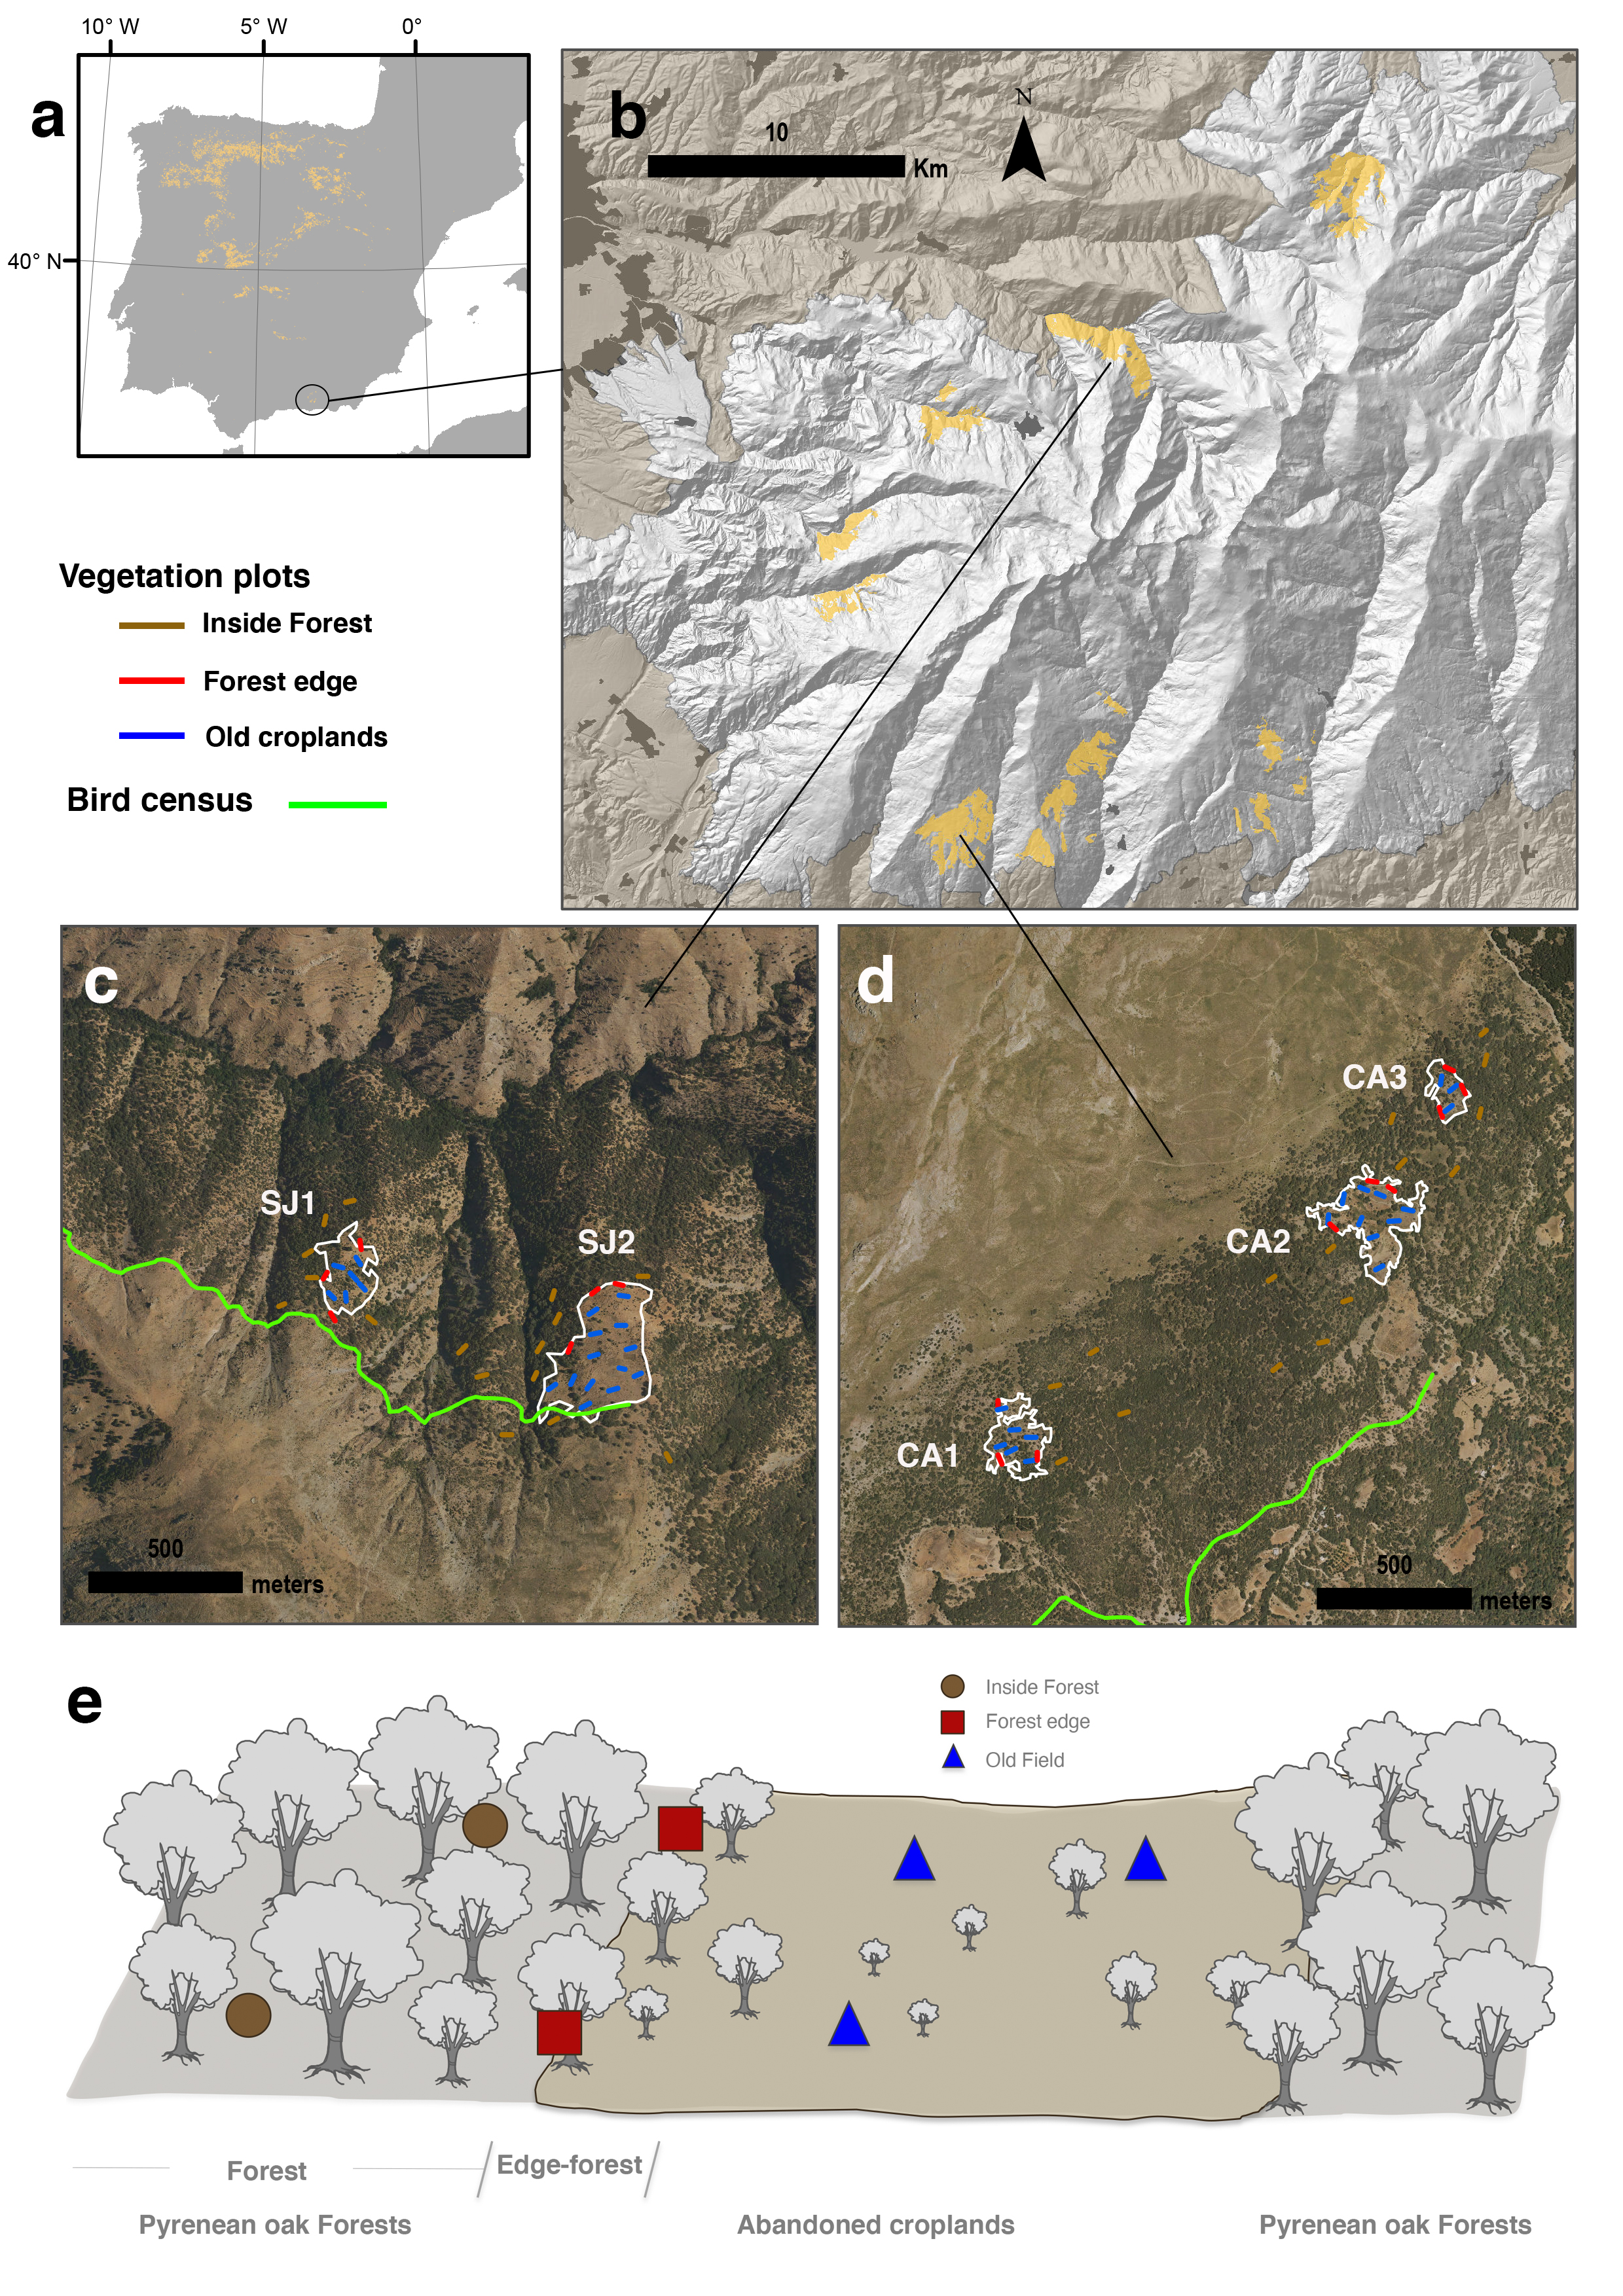
\includegraphics[width=\textwidth,height=16cm,
  keepaspectratio]{img/coloniza/coloniza-map.jpg}
    \caption{Distribution of \Qp forests in the Iberian Peninsula (a), and in Sierra Nevada mountain range (b). Location of the old croplands (\emph{white} lines) in the study sites: Robledal de San Juan (SJ) (c), and Robledal de Cáñar (CA)(d). Names of the old croplands as in \tabref{tab:coloniza:croplands}. Sampling design (e). Vegetation plots were randomly placed in the abandoned croplands (triangles), and inside the forest (circles) surrounding the old field. Several plots were also located at forest-old field edge (squares).}
    \label{fig:coloniza:transects}
\end{figure}


\Qpw woodlands, like other forest formations in the Mediterranean region, have been subjected to intense anthropogenic pressures over time \autocites{GarciaJimenez20099230Robledales, AlbaSanchezetal2021EarlyAnthropogenic}, which have led to the reduction of their distribution area, as well as to the modification of their floristic and structural patterns \autocites{Gavilanetal2000EffectsDisturbance,Calvoetal1999PostfireSuccession,Tarregaetal2006ForestStructure}. Historically, the woodlands of \Qp have been exploited mainly for firewood, charcoal, and tannins \autocites{RuizdelaTorre2006FloraMayor,SanchezPalomaresetal2008EstacionesEcologicas}. Some areas were also burned and thinned to create pastures with low densities of mature trees that provide acorns, firewood, and large areas for grazing \autocites{HerreraCalvo2016UsoPastoral,Alvarezetal2009CambiosEstructura,ValbuenaCarabanaGil2017CentenaryCoppicing}. All these anthropogenic processes have transformed the oak woodlands in a deep way that it is difficult to find stands that can be considered natural forests \autocites{RuizdelaTorre2006FloraMayor}. Nonetheless, the decrease in anthropogenic pressure has paradoxically caused that many of the \Qp oak stands present a state of advanced degradation, showing growth stagnation, lack of fruiting, and also symptoms of branch dieback  \autocites{Canellasetal2004GrowthResponse, Bravoetal2008SelviculturaMontes, ValbuenaCarabanaGil2014EfectosGestion, PiqueVericat2015EvolutionPerspectives, Piqueetal2018Spain}. 

Therefore, understanding the woodland expansion towards abandoned croplands would become critical to develop effective management strategies, particularly for populations representing the rear-edge of their distribution \autocite{HampePetit2005ConservingBiodiversity} which need a particular attention due to their high conservation value \autocite{Fadyetal2016EvolutionbasedApproach}.  
The study of ecological dynamics within the rear-edge populations is considered essential to establish proper management guidelines under current climate uncertainties \autocites{Fadyetal2016EvolutionbasedApproach,Jumpetal2010MonitoringManaging}. Rear-edge populations are often adapted to local environmental conditions at the limit of the species ecological amplitude, and often show a long-term persistence \autocite{HampePetit2005ConservingBiodiversity}. Local responses to environmental changes may differ from the species mean response \autocites{Benavidesetal2013DirectIndirect,Matiasetal2017ContrastingGrowth,Castroetal2004SeedlingEstablishment}, and such differences may either promote or hamper the survival of edge populations under global change \autocites{Fadyetal2016EvolutionbasedApproach,Jumpetal2010MonitoringManaging}. In this work we analyze the colonization pattern of abandoned croplands by \Qpy in Sierra Nevada mountain region. This mountain has undergone significant land use changes in the last 50 years \autocites{JimenezOlivenciaetal2015EvolucionUsos} with increases of forest densities \autocite[see chapter \ref{sec:carbon}; also][]{JimenezOlivenciaetal2015MedioSiglo}, and tree growth \autocite[see chapter \ref{sec:dendro};][]{PerezLuqueetal2020LanduseLegacies}. We are interested in exploring the colonization pattern of abandoned croplands by \Qp on both slopes of the Sierra Nevada. We aimed to assess differences among populations in the rear edge of its distribution. Our specific goals are \emph{(i)} to analyze the colonization pattern of abandoned cropland by \Qp and its relationship with time after abandonment; \emph{(ii)} to explore differences on the structure of the seed source (mature woodlands); and \emph{(iii)} to compare the abundance of the main seed disperser (Eurasian jay, \emph{Garrulus glandarius}).

\section{Material and Methods}\label{sec:coloniza:MatMet}
\subsection{Sampling description}\label{sec:coloniza:sampling}

\begin{table}
\caption{Main characteristics of the abandoned croplands studied.}
\centering
\resizebox{\linewidth}{!}{
\begin{tabular}[t]{cc>{\centering\arraybackslash}p{8em}ccccc}
\toprule
\multicolumn{1}{c}{ } & \multicolumn{2}{c}{Cropland} & \multicolumn{2}{c}{ } & \multicolumn{3}{c}{Number of plots} \\
\cmidrule(l{3pt}r{3pt}){2-3} \cmidrule(l{3pt}r{3pt}){6-8}
Site & Code & Abandonment Age (years) & Elevation (m) & Area (ha) & Cropland & Edge & Forest\\
\midrule
 & CA1 & > 60 & 1796-1866 & 3.29 & 6 & 3 & 4\\
\cmidrule{2-8}
 & CA2 & < 30 & 1789-1858 & 5.80 & 9 & 3 & 7\\
\cmidrule{2-8}
\multirow{-3}{*}{\centering\arraybackslash Robledal de Cáñar} & CA3 & 40 - 60 & 1851-1892 & 1.56 & 3 & 3 & 4\\
\cmidrule{1-8}
 & SJ1 & 40 - 60 & 1507-1674 & 3.47 & 6 & 3 & 6\\
\cmidrule{2-8}
\multirow{-2}{*}{\centering\arraybackslash Robledal de San Juan} & SJ2 & 30 - 40 & 1575-1746 & 10.36 & 13 & 3 & 10\\
\bottomrule
\end{tabular}}
\label{tab:coloniza:croplands}
\end{table}

We sampled 5 abandonment croplands located at two Pyrenean oak forests in contrasting slopes of Sierra Nevada (southern Spain): Robledal de San Juan (SJ), located at the northern aspect (37°7'29.63"N, 3°21'54.60"W; Güejar-Sierra, Granada, Spain); and Robledal de Cáñar (CA), located at the southern aspect (37°57'28.04"N, 3°25'57.1"W; Cáñar, Granada). We selected oak populations located at contrasting slopes since differences in environmental variables have been reported for those oak woodlands \autocite{PerezLuqueetal2021EcologicalDiversity}. Each cropland was delimited using land-use and land-cover map of Andalusia for 1956 \autocites[][]{CMA2007MapaUsos} combined with a detailed photographic interpretation of the black and white 1956 orthophotos (1-m spatial resolution) \autocites[see][for more details]{NavarroGonzalezetal2012CartografiaHistorica}. The estimation of the age abandonment for each cropland were performed combining intrepretation of orthophotographies with information from local neighbors. We compiled all available aerial ortophotographies of the study areas from Fototeca Digital of the Spanish National Geographic Institute (\href{http://fototeca.cnig.es/}{http://fototeca.cnig.es/}). These dates were verified using information about past land-use, compiled from local neighbours \autocites[by local workshops and interviews with retired elder: farmers, shepherds and loggers; see details in ][]{MorenoLlorcaetal2014CaracterizacionFuentes,MorenoLlorcaetal2016HistoricalAnalysis}. The estimated rank of ages could be considered accurate (see \tabref{tab:coloniza:croplands}).

For each abandonment cropland, vegetation plots (30 m x 10 m) were randomly distributed in the old field; at the forest edges; and inside the surrounding forests (\figref{fig:coloniza:transects}). The number of plots within the old fields and surrounding forests were proportional to the size of the abandonment cropland (\tabref{tab:coloniza:croplands}). A total of 83 vegetation plots were sampled in autumn 2012. In each vegetation plot all tree species were recorded, and tree height and diameter were measured. For each transect we computed the juvenile abundance as the number of individuals smaller than 150 cm on height. We did not distinguish the reproductive and vegetative origins of young oaks, since it is difficult due to the resprouting trait of this species. In addition to the juvenile abundance, we explored differences between several recruitment stages based on individual size \autocites[\emph{e.g}][]{Plieningeretal2010LargeScalePatterns}. We considered five size categories based in height (every 30 cm). All data were properly documented and published in an international repository \autocites[see][for a detailed description of the dataset]{PerezLuqueetal2015DatasetMIGRAME}. 
To explore the main bird disperser in our study sites, we used bird censuses carried out by the Sierra Nevada Global Change Observatory (\href{https://obsnev.es/}{https://obsnev.es/}). This dataset contains bird censuses at different ecosystems types of Sierra Nevada since 2008 \autocites[for more details see][]{BareaAzconetal2012PasseriformesOtras, PerezLuqueetal2016DatasetPasserine}. We only used data for the Eurasian jay (\emph{Garrulus glandarius}), since it is the main disperser of \Qpy \autocites{Gomez2003SpatialPatterns}. We assumed that jays can move acorns into abandoned croplands based on the habitat-preferences to cache acorns reported by \citet{PonsPausas2007AcornDispersal}, and also considering preliminary data on jays flights carried out in our study sites by \citet{Zamoraetal2013CambioGlobal}, who found a high proportion of flights of this bird at the same elevation, and around 40\% of open areas as arrival habitat. Since we were interested in the comparison of the Eurasian jay populations between the two study sites, we computed the annual bird abundances (in terms of birds/10 ha) for each site during a 7-year period (2008-2013). The sampling procedures was the line-transect method with a bandwith of 50 m (25 m on each side). Transects length were 2.80 km for Cáñar site (CA), and 3.22 km for San Juan site (SJ). Sight and sound records within the sample area were accepted as contacts. All transects were sampled in the early morning. Eurasian jay abundance was calculated in terms of birds/10 ha. All counts in one month were averaged, and the yearly result was obtained from the average of all the months studied. For more details about bird censuses see \citet{BareaAzconetal2012PasseriformesOtras} and \citet{ZamoraBareaAzcon2015LongTermChanges}.


\subsection{Data analysis}\label{sec:coloniza:analysis}
We used the vegetation plots carried out inside the forest (habitat type = forest) to analyze the structure of the seed source (surrounding forest). Several parameters related to forest structure and functioning were computed: tree density, juvenile abundance, tree species composition, tree size related statistics (\emph{i.e.} mean, median, maximum, 75 and 90 percentiles of tree-height), and basal area (BA). Differences between sites were assessed using the non-parametric Mann–Whitney U-test, since data did not meet normality nor/either homocedasticity assumptions. We also compared whether there was variation within plots belonging to the same sites. ANOVA analyses were performed to explore differences of bird disperser abundance (\emph{G. glandarius}) between sites and across years. 

The variation of the juvenile abundance between study sites, habitat type, and their interaction (site-habitat type), was analyzed using Generalized Linear Models with a Tweedie distribution with a log link \autocite{DunnSmyth2018TweedieGLMs}. Study sites and habitat type were the explanatory variables. Prior to the analysis, data exploration was applied following protocols described by \citet{Zuuretal2010ProtocolData} and \citet{IenoZuur2015BeginnerGuide}. As the dataset comprised count data, we initially used the Poisson and the Negative Binomial distribution. However, these models were overdispersed. A variance power parameter of 1.28 (1.20-1.40, 95\% confidence interval) were used in the Tweedie GLM model. This parameter was estimated using the \texttt{tweedie.profile} function of the \texttt{tweedie} R package \autocites{DunnSmyth2005SeriesEvaluation,Dunn2017Tweedie}. Model comparison (univariate models) was carried out using the Akaike's information criterion (AIC) \autocites{BurnhamAnderson2010ModelSelection}. The model accuracy was tested by Nagelkerke's pseudo-$R^2$, used as a measure of goodness of fit. The significance of the explanatory variables in the selected model was tested using the likelihood ratio tests (LRT). Wald z-tests and Tukey's HSD-corrected \emph{post hoc} comparisons were used to test for differences in juvenile abundance among sites and habitat-type. 

\begin{table}
\caption{Forest attributes of northern (SJ) and southern (CA) sites. U Mann-Withney statistics with significance at 0.05 level. Mean and SE are shown}
\centering
\resizebox{\linewidth}{!}{
\begin{tabular}[t]{ccccc}
\toprule
Variable & Southern site (CA) & Northern site (SJ) & U statistic & p value\\
\midrule
\% of Q. pyrenaica & 96.11 ± 1.28 & 100 ± 0 & 3.688 & 0.0001\\
Tree density (ind/ha) & 1671.11 ± 229.21 & 1587.5 ± 161.67 & 4.808 & 0.9369\\
Juvenile abundance (ind/ha) & 1004.44 ± 195.72 & 883.33 ± 127.18 & 4.852 & 0.7667\\
Adult abundance (ind/ha) & 584.44 ± 80.47 & 704.17 ± 63.31 & 4.448 & 0.1780\\
Maximum tree height (m) & 13.93 ± 0.65 & 13.75 ± 0.71 & 4.824 & 0.8736\\
Tree height mean (m) & 4.32 ± 0.6 & 5.09 ± 0.37 & 4.330 & 0.0855\\
Tree height median (m) & 3.19 ± 0.83 & 3.57 ± 0.66 & 4.564 & 0.3527\\
Tree height 75 percentile (m) & 5.73 ± 1.02 & 8.29 ± 0.6 & 4.343 & 0.0922\\
Tree height 90 percentile (m) & 10.07 ± 0.95 & 11.22 ± 0.54 & 4.605 & 0.4399\\
Basal Area (m2/ha) & 37.56 ± 4.23 & 33.58 ± 3.6 & 4.912 & 0.5400\\
\bottomrule
\end{tabular}}
\label{tab:coloniza:forest}
\end{table}

\begin{table}[]
\caption{Model selection for the oak juvenile abundance, sorted by minimum AICc value.}
\resizebox{\textwidth}{!}{%
\begin{tabular}{@{}llllll@{}}
\toprule
\textbf{model.name} & \textbf{df} & \textbf{logLik} & \textbf{AICc} & \Delta \textbf{AICc} & \textbf{Nagelkerke R\textsuperscript{2}} \\ \midrule
Habitat type + Site + Habitat type \(\times\) Site & 6 & -221.89 & 457.78 & 0 & 0.970 \\
Habitat type + Site & 4 & -231.83 & 473.65 & 15.87 & 0.955 \\
Habitat type & 3 & -236.21 & 480.42 & 22.64 & 0.946 \\
Site & 2 & -291.06 & 588.12 & 130.34 & 0.116 \\
null model & 1 & -293.09 & 590.19 & 132.41 & 0 \\ \bottomrule
\end{tabular}%
}%
\label{tab:coloniza:modelselection}
\end{table}

\section{Results}\label{sec:coloniza:results}

The forest structure of \Qpy woodlands did not show significant differences for the forest attributes between study sites  (\tabref{tab:coloniza:forest}). \Qpy woodlands of southern site (CA) showed higher tree density but smaller tree heights (mean, median and percentiles) than those on the northern site (SJ) (\tabref{tab:coloniza:forest}). In addition, higher abundance of juveniles was found for CA site, which also showed greater basal area than SJ site (\tabref{tab:coloniza:forest}).

Regarding the abundance of \emph{Garrulus glandarius}, no differences between study sites were found (\(F_{1,82}\) = 2.387; p = 0.126; CA = 1.69±0.21 and SJ = 1.33±0.22 birds/10ha), neither across years in the studied period (2008-2014) (\(F_{6,82}\) = 1.234; p = 0.297). The interaction term was also not significant (\(F_{6,82}\) = 1.26; p = 0.284).

\begin{figure}[H]
    \centering
    \includegraphics[width=\textwidth,height=8cm,
  keepaspectratio]{img/coloniza/coloniza-juvenile-interaction.pdf}
    \caption{Interaction plot for the oak juvenile abundance. Habitat-type differences within each site were indicated with different letters. Differences between sites for each habitat-type were indicated with asterisk. CA: \emph{Robledal de Cáñar} site (southern slopes); SJ: \emph{Robledal de San Juan} site (northern slopes).}
    \label{fig:coloniza:interaction}
\end{figure}

The juvenile oak abundance model including all terms (\emph{i.e.} full model) showed higher strength of empirical support than did models for each of the independent variables (\emph{i.e.} univariate models) (\tabref{tab:coloniza:modelselection}). Oak juvenile abundance differed among habitat types (\(F_{2,77}\) = 72.95; p < 0.0001), and between study sites (\(F_{1,77}\) = 8.16; p = 0.0054; \tabref{tab:coloniza:anova}). 

A decreasing gradient of oak-juvenile abundance was found across habitat-type, from higher values in forest type (15.90 ± 1.30 \juv) to lower values inside the old croplands (2.43 ± 0.55 \juv; \figref{fig:coloniza:interaction}). The abundance of oak juveniles in the old croplands of the southern site (CA) was significantly higher (4.06 ± 0.98 \juv) than in those of the northern site (SJ; 0.90 ± 0.26 \juv). 

The size distribution of juveniles was also different among the study sites (\figref{fig:coloniza:treeCategory}). An even size-distribution of the oak juveniles was observed in the old croplands of northern site. Conversely, higher contribution of small oak juveniles (< 30 cm) were found at old croplands of southern site (\figref{fig:coloniza:treeCategory}). 

A positive relation was found between the oak juvenile abundance and the estimate age of crop abandonment (\figref{fig:coloniza:ageCrop}) with higher oak juvenile abundances in the earlier abandoned croplands 

\section{Discussion}\label{sec:coloniza:disussion}

\begin{table}
\footnotesize
\caption{ANOVA table of the selected GLM model for the abundance of \Qpy juvenile across study sites and habitat types. F-value and p-values are displayed.}
\centering
\begin{tabular}{lllll} 
\toprule
\textbf{Variable}        & \textbf{SS} & \textbf{df} & \textbf{F} & \textbf{p-value}  \\ 
\midrule
Habitat type             & 233.89      & 2           & 72.95      &  0.0001           \\
Site                     & 13.09       & 1           & 8.16       & 0.0054            \\
Habitat type $\times$ Site & 27.19       & 2           & 8.48       & 0.0004            \\
Residuals                & 123.43      & 77          &            &                   \\
\bottomrule
\end{tabular}
\label{tab:coloniza:anova}
\end{table}


We observed a colonization process of \Qpy into abandoned croplands in this mountain region despite the strong recruitment constraints described for this species \autocites{Bravoetal2008SelviculturaMontes,Gomez2003ImpactVertebrate,Pereaetal2014InteraccionesPlantaanimal}. Forest expansion towards abandoned croplands has been recorded in several marginal habitats in other European mountainous regions \autocites{Amezteguietal2016LanduseLegacies,Nataleetal2007StudyTree,Piussi2000ExpansionEuropean,Amezteguietal2010LanduseChanges,LasantaMartinezetal2005MountainMediterranean,Kozak2003ForestCover,AlvarezMartinezetal2014InfluenceLand,VicenteSerranoetal2004AnalysisSpatial}, as consequence mainly of rural depopulation and decrease on herbivores pressure \autocite{MacDonaldetal2000AgriculturalAbandonment,EuropeanEnvironmentAgency2016EuropeanForest}. Our results show a relationship between juvenile-oak abundance and the estimated age of crop abandonment (\figref{fig:coloniza:ageCrop}). As the time after crop abandonment increases, species heterogeneity and functional diversity of the ecosystem increases \autocites{PuertaPineroetal2012HistoryMatters,HermyVerheyen2007LegaciesPresentday}, boosting the multifuntionality of the ecosystems \autocite{CruzAlonsoetal2019LongTerm}. 

\begin{figure}
    \centering
    \includegraphics[width=\textwidth,height=10cm,
  keepaspectratio]{img/coloniza/coloniza-TreeCategory.pdf}
    \caption{Juvenile abundance classified by tree-size (see material and methods) by habitat-type in the two study sites. Mean and standard error are shown.}
    \label{fig:coloniza:treeCategory}
\end{figure}

It has been also reported that both age of the surrounding forests and previous land use could influence the colonization pattern \autocite{MinottaDegioanni2011NaturallyRegenerated}. In this sense, it is expected that the colonization process will continue, since the forests surrounding our study areas are relatively young. Dendrochronological estimates of the forest age for our study woodlands, ranged approximately 90-100 and 200 years for northern and southern oak populations respectively \autocite{PerezLuqueetal2020LanduseLegacies, GeaIzquierdoCanellas2014LocalClimate}, which is younger than the estimated ages for these forests along their distribution range \autocites{GeaIzquierdoCanellas2014LocalClimate}. \citet{CruzAlonsoetal2019LongTerm}, in a study of the recovery of multifunctionality in Mediterranean forests, reported for this oak species, a minimum of 80 years after the abandonment for the recovery of the reference multifunctionality. 

The colonization pattern of abandoned croplands varies within the rear-edge of the \Qp. Our results showed different abundances of oak juveniles between sites, with higher abundances at the southern sites (CA) (\tabref{tab:coloniza:anova}; \figref{fig:coloniza:interaction}). It is known that the distance to the source and the structure of the seed source influenced the propagule input into new habitats \autocites{Nathan2006LongDistanceDispersal,HewittKellman2002TreeSeed,Kureketal2019DispersalDistance}. In our study sites, all the abandoned croplands are surrounded by native forests. Thus, the observed differences in oak juvenile abundance would not seem explained by the distance to the seed source (\tabref{tab:coloniza:croplands}). Regarding to the structure of the seed source, we found no differences between the study sites (\tabref{tab:coloniza:forest}). Forest attributes potentially related to the acorn production \autocite[\emph{e.g.} tree density, basal area,][]{GeaIzquierdoetal2006AcornProduction} are not different for surrounding forests between study sites (\tabref{tab:coloniza:forest}). Although in our work we have not carried out an estimation of acorn production that would allow us to compare between study sites, previous studies analyzing the variation in reproductive parameters and comparing the acorn production across oak woodlands of Sierra Nevada, found slight differences among oak populations, with higher acorn yield for southern oak woodlands than northern one \autocite{Leal2013AnalisisCrecimiento}.  However, the data series used by \citet{Leal2013AnalisisCrecimiento} was very short (only two years) and \Qpy have a marked mast-seeding behaviour \autocites{Bravoetal2008SelviculturaMontes,Gomezetal2001ProblemasRegeneracion}. Besides that, there not seem to be marked differences in the current seed source that could explain our observed differences in the abundance of juveniles in the abandoned crops. 

\begin{figure}
    \centering
    \includegraphics[width=\textwidth,height=6cm,
  keepaspectratio]{img/coloniza/coloniza-ageCrop.pdf}
    \caption{Relation of the juvenile oak abundance with the estimated age of crop abandonment.}
    \label{fig:coloniza:ageCrop}
\end{figure}

Another key aspect for the tree colonization of abandoned croplands is the dispersion vectors. \Qp acorn are mainly dispersed by woodmouse (\emph{Apodemus sylvaticus}) and Eurasian jay (\emph{Garrulus glandarius})\autocites{Gomez2003ImpactVertebrate,Pereaetal2014InteraccionesPlantaanimal}. We used a time series (a 7-year period) to analyze the abundance of jays at each study site. The aim of using this time series was to explore whether there were differences between study sites with respect to the abundance of this bird acorn-disperser. We are aware of the limitation of using these data, \emph{i.e.} we do not know if the abundance of jays at both sites has followed the same temporal trajectory, but we have used the longest time series we have for both sites, to at least find out if there are differences between the sites in recent years. Our results showed similar abundances of this acorn disperser between the two study sites. Therefore, the observed differences in oak juvenile abundance do not appear to be explained by differences in abundance of this acorn disperser. Having observed no differences in the seed source neither in the main dispersal vector, a logical next step would be to explore differences on the seed arrival site. 

For the recolonization of abandoned croplands, besides the importance of factors related to dispersal in time (seed bank related) and space (distance related), the previous use to which the crop field has been subjected is a key factor determining the abundance of native tree species \autocites{HermyVerheyen2007LegaciesPresentday,NavarroGonzalezetal2013WeightLanduse}. The colonization pattern of woody species is affected by fine-scale variations in abiotic factors \autocite{Milderetal2013ColonizationPatterns,Leverkusetal2016ShiftingDemographic}, but it has been observed that land-use history mainly controlled the forest expansion rates \autocites{AlvarezMartinezetal2014InfluenceLand,Perringetal2016GlobalEnvironmental}. The forest history of our study sites, inferred from several compiling studies \autocites{MorenoLlorcaetal2014CaracterizacionFuentes, Titos1990, PerezLuqueetal2020LanduseLegacies,MorenoLlorcaetal2016HistoricalAnalysis,MesaTorres2009,JimenezOlivenciaetal2015EvolucionUsos}, indicated that both sites were subjected to intense anthropic uses in the past. At the northern site (SJ), uplands areas were dedicated to grazing, and in the forest areas there were also some croplands with grazing. In addition, timber extraction for mining were recording at this site. Southern site (CA) has been exploited for firewood, charcoal and acorns, with less presence of livestock use. Although we could not estimate the intensity of use to which both zones have been subjected before the abandonment of crops, the northern zone seems to have had a management history with higher grazing intensity than the southern site \autocite{MorenoLlorcaetal2016HistoricalAnalysis, MorenoLlorcaetal2014CaracterizacionFuentes,MorenoLlorcaZamora2012CaracterizacionCarga}. 

In addition to the land-use legacies previous to the cropland abandonment, another relevant question would be the management history after the crop cessation, focusing on the livestock pressure, since herbivory impose severe constraints to the establishment and regeneration of this oak species \autocites{Gomez2003ImpactVertebrate, Pereaetal2014InteraccionesPlantaanimal}. There is no data available on the temporal evolution of grazing pressure at detailed scale in our study sites. Only \citet{RoblesCruz2008ConjuntoSierras} showed an general quantification for several ecosystems of Sierra Nevada. Notwithstanding, several studies and reports, combining interviews with shepherds and reviewing of historical documents, have determined the recent livestock history in several oak woodlands of the Sierra Nevada \autocites{MorenoLlorcaetal2016HistoricalAnalysis, MorenoLlorcaetal2014CaracterizacionFuentes,MorenoLlorcaZamora2012CaracterizacionCarga}. For our study sites it has been observed both higher numbers of herds and sheperds, and more livestock density in the northern site (SJ) than in the southern one (CA), which could be translated into a greater herbivore pressure that would explain our observed differences in juvenile oak abundance within the abandoned croplands. This distinct herbivory pressure in the two study sites could explain the differences observed in the juvenile oak abundance not only at cropland habitat type either both at edge and forest habitat type. The exploration of abundance juveniles by size categories between habitats type for each study site showed lower abundance values for northern site (\figref{fig:coloniza:treeCategory}). The size-age structure is also more homogeneous at the northern site, reinforcing the hypothesis of higher herbivore pressure. \citet{Gomez2003ImpactVertebrate} found that herbivory rather than abiotic factors is the main cause of seedling mortality of \Qp in Sierra Nevada. Thus, herbivores killed most of the seedlings, although the way in which they severed the seedlings was very diverse \cite{Gomez2003ImpactVertebrate}. They found that trampling by livestock and acorn predation by wild boards and hares were the main causes of the mortality observed, but the browsing by livestock is marginal (only 1\% of the mortality) \autocite{Gomez2003ImpactVertebrate}. Another factor to consider is the presence of shrubs which can act as nurse plants. Facilitation by nurse plants has been reported as an essential process for the regeneration of some tree species  \autocites{Castroetal2006RestoringQuercus,GomezAparicioetal2004ApplyingPlant}. The survival of \Qp substantially increases when it is under individual pioneer shrubs \autocite{Castroetal2006RestoringQuercus,Costaetal2017CanNative}. Shrubs may protect \Qp seedlings from browsing and trampling of vertebrate herbivores. They also offer safe sites that reduce the high mortality rates during the summer in the early stages of recruitment \autocites{Castroetal2006RestoringQuercus,Barazaetal2004HerbivoryHas}. Although we did not estimate the cover and diversity of shrub species in our studied abandoned crops, previous studies in the surrounding forests of the same localities did not found differences in the diversity and richness of shrubs within oak forests \autocite{Munoz2012BosquesAutoctonos}. 

\section{Concluding remarks}\label{sec:coloniza:Conclusion}
The results of our study show that, even in the current increasingly dry climatic conditions, \Qp woodlands are able to recover the abandoned former arable fields at the same altitudinal level where oak woodland is the potential vegetation. Thus, the Pyrenean oak woodland is clearly expanding in Sierra Nevada mountain range, a rear edge of the distribution of this oak species. This natural process can provide solutions for conservation of biodiversity, and enhances the mitigation of, and the adaptation to climate change \autocites[][and references therein]{Chazdonetal2020FosteringNatural}. Besides this, active restoration could aid to recovery the oak forest multifunctionality \autocite{CruzAlonsoetal2019LongTerm} in the abandoned croplands that are being colonized by tree species.

The differences in the recolonization patterns within the rear-edge seems be related to differences in the management prior to and after abandonment of mountain croplands. A higher herbivory pressure after cropland abandonment seems to limit the forest expansion towards marginal habitats. Related to this, and in order to improve the forest expansion, it would be recommended to take advantage of the presence of native shrubs that offer safe sites. Those safe sites could aid to reduce the mortality of \Qp seedlings, and therefore increase the establishment probabilities of this oak species. This also would aid to increase heterogeneity within the ongoing secondary forest, which also increase the resilience to perturbations y the recovery of the ecosystem multifunctionality \autocite{Stritihetal2021ImpactLanduse, CruzAlonsoetal2019LongTerm}. On the other hand, attention also is needed to maintain healthy seed sources (surroundings forests), and a stable seed disperser community, particularly the Eurasian jay, since acorn dispersion by this bird species is considered a key process in the regeneration of \emph{Quercus} forests after land abandonment \autocite{Pausasetal2006RegenerationMarginal}.
  
% !TEX root = ../my-thesis.tex
%
%\selectlanguage{english}  
\chapter{Carbon sequestration of coppiced forests of \Qpy. An study case from the rear-edge of its distribution}\label{sec:carbon}

\mbox{}
\vfill
{\color{ctcolormain}\textbf{Antonio J. Pérez-Luque}}; Mihai Tanase; Cristina Aponte \& Regino Zamora (In prep.)


\newpage

\paragraph{Abstract} \mbox{} \\

\newpage

\section{Introduction}\label{sec:carbon:intro}

Forest ecosystems are suppliers of several ecosystems services to humans \autocite{Iversonetal2018EcosystemServices,MartinezPasturetal2018EcosystemServices,NoceSantini2018MediterraneanForest}. Forest ecosystem services include provisioning services (\emph{e.g.} wood and non-wood forest products), regulating services (\emph{e.g.} climate regulation), habitat or support services, and cultural services. In Mediterranean region, humans have been exploiting forest resources for centuries \autocite{ValbuenaCarabanaetal2010HistoricalRecent}, however in the last decades a strong abandonment of traditional activities in mountains regions have been observed, mainly due to the rural exodus and the low economic value of forest products activities \autocite{Chauchardetal2007PatternsLanduse,Debusscheetal1999MediterraneanLandscape,MacDonaldetal2000AgriculturalAbandonment}. As a result, many forests currently have high tree-density stands, with an increased competition for resources, which can lead to widespread weakening of stand, increasing the vulnerability of forests to abiotic and biotic disturbances \autocite{Tardieuetal2018HumanNeeds}. This may be especially relevant for forests stands located at the rear-edge of the species distribution \autocite{HampePetit2005ConservingBiodiversity}, which are usually considered more vulnerable to climate change compared with populations at the centre of a species' range \autocite{Fadyetal2016EvolutionbasedApproach,Pirononetal2017GeographicVariation,Rehmetal2015LosingYour}.

\Qp (Pyrenean oak) is a deciduous Mediterranean tree species widely distributed throughout southwestern France and the Iberian Peninsula, reaching their southern limit in mountain areas of northern Morocco \autocite{Franco1990Quercus}. The rear-edge populations of this species are restricted to high-mountain areas where these populations persists as isolated nuclei with ecological conditions very different from those of the main distribution area \autocite{PerezLuqueetal2021EcologicalDiversity}. Due to its ability to resprout from stumps and the entire root system, most stands of this species have been coppiced for centuries mainly for firewood, charcoal, tannins and woody pasture production \autocite{SanchezPalomaresetal2008EstacionesEcologicas,XimenezdeEmbun1961MonteBajo}. All these anthropogenic processes have transformed native woodland structures \autocite{Tarregaetal2006ForestStructure}, and nowadays it is difficult to find stands of this oak that can be qualified as natural or pristine forests \autocite{RuizdelaTorre2006FloraMayor}. Paradoxically, after the diminution of human pressure on woodlands over the last decades, the abandoned coppices of \Qp present an advanced state of degradation with important ecological, economic and social problems \autocite{Bravoetal2008SelviculturaMontes,MontoyaMeson1979SituacionActual,Piqueetal2018Spain,PiqueVericat2015EvolutionPerspectives,Vericatetal2012GestionAdaptativa}. Due to the importance of this species, several studies have proposed management practices (e.g.~conversion to high forest) to improve the state of abandoned coppices \autocite{Bravoetal2008SelviculturaMontes,Montoya1982SelviculturaOrdenacion,Montoya1983UsosAlternativos,Serradaetal1992CoppiceSystem,Vericatetal2012GestionAdaptativa}, although they have not been very successful, partly due to the lack of a comprehensive understanding of the physiological mechanisms underpinning tree stagnation \autocite{Salomonetal2017GeneralFailure,ValbuenaCarabanaGil2017CentenaryCoppicing}. In view of this situation, it is essential to seek for alternative management practices to the traditional uses of the abandoned coppices \autocite{MesonMontoya1985VegetacionForestal,SanMigueletal2012BosquesMatorrales}. Some management alternatives based on pastoral use have been proposed \autocite{HerreraCalvo2016UsoPastoral}, but to our knowledge few proposals have focused on the provision of the ecosystem services provided by this oak forests \autocites[but see][]{Piqueetal2018Spain,PiqueVericat2015EvolutionPerspectives}.

The carbon sequestration is one of the most relevant ecosystems services provided by Mediterranean forests \autocite{Gauquelinetal2018MediterraneanForests,NoceSantini2018MediterraneanForest}. Carbon stock can be assumed as an indicator of the capacity of ecosystems to contribute to climate regulation because their potential to influence atmospheric CO\textsubscript{2} concentration \autocite{Lauterbach2007AssessmentExisting,Luyssaertetal2008OldgrowthForests}. Mediterranean forests represent a carbon sink expected to increase over coming decades \autocite{Canellasetal2017CarbonSequestration,PasalodosTatoetal2017EvaluationTree}. Improving carbon estimation and our understanding of the effects of forest management could be useful for forest managers, which could include carbon sequestration among the different objectives pursued in the management \autocite{RuizPeinadoetal2017ForestManagement}. Several studies have been conducted to determine carbon sequestration by forest ecosystems in the Mediterranean region based on data from forest carbon inventories, field measurements, remote sensing, laser scanning and growth simulation \autocites[\emph{e.g.}][]{Canellasetal2008SilvicultureCarbon,Chiesietal2005ModellingCarbon,Garciaetal2010EstimatingBiomass,GuerraHernandezetal2016ComparisonALS,Simonsonetal2016ModellingAboveground,Vayredaetal2012SpatialPatterns}. LIDAR (Light detection and ranging) has emerged as an effective technique for quantifying aboveground biomass in forests \autocite{Belandetal2019PromotingUse,Lefskyetal2002LidarRemote,Xiaoetal2019RemoteSensing} and has been also used for quantifying carbon stocks \autocite{Simonsonetal2016ModellingAboveground,Zhaoetal2018UtilityMultitemporal}. In this study we combined Airborne Laser Scanning LIDAR data and field inventories to estimate the biomass of Pyrenean oak woodlands (\Qp) of Sierra Nevada (southern Spain), and then to assess the carbon sequestration capacity of those forests and their role as carbon sink. The specific objectives are: \emph{(i)} to generate biomass cartography of the oak woodlands of Sierra Nevada using field inventories and LIDAR data; \emph{(ii)} to estimate the potential capacity of these ecosystems to sequester carbon dioxide, and the temporal trends for this ecosystem service; \emph{(iii)} to analyse the differences in biomass and carbon sequestration among oak populations within this mountain region; \emph{(iv)} and to explore the factors that explain the C stock for \Qp woodland in Sierra Nevada.

\section{Material and Methods}\label{sec:carbon:mat}
\subsection{Study site and oak woodlands}\label{sec:carbon:mat-studysite}

\Qpy forests extend throughout south-western France and the Iberian Peninsula, reaching their southern limit in mountain areas of northern Morocco \autocite{Franco1990Quercus}. In the Iberian Peninsula, these forests occupy siliceous soils under meso-supramediterranean and mesotemperate areas and subhumid, humid, and hyperhumid ombroclimate. The forests of this species reach their southernmost European limit in Andalusian mountains such as Sierra Nevada (37°N, 3°W), a high-mountain range with elevations of up to 3 482 \emph{m a.s.l.}. The climate is Mediterranean, characterized by cold winters and hot summers, with pronounced summer drought and increasing aridity with decreasing altitude, and marked variability according to elevation and aspect. In Sierra Nevada, there are eight Pyrenean oak populations (2 400 ha), from 1 100 to 2 000 \emph{m a.s.l.} and often associated with major river valleys. Those oak populations have been grouped in three oak-population clusters, based on their forest structure and floristic: the northern (N), the northwestern (NW), and the southern (S) clusters \autocite{PerezLuqueetal2021EcologicalDiversity}. \emph{Quercus pyrenaica} woodlands in this mountain region represent a rear edge of their habitat distribution \autocite{HampePetit2005ConservingBiodiversity}. They are the richest forest formation in vascular plant species of Sierra Nevada, containing several endemic and endangered plant species \autocite{Loriteetal2008PhytosociologicalReview}, and they also harbor high levels of intraspecific genetic diversity \autocite{ValbuenaCarabanaGil2013GeneticResilience}. However, these relict forests have undergone intensive human use throughout history \autocite{CamachoOlmedoetal2002DinamicaEvolutiva}. Furthermore, the conservation status of this species for southern Spain is considered Vulnerable and it is expected to suffer from climate change, reducing its suitable habitats in the near future \autocite{GeaIzquierdoetal2013GrowthProjections,GeaIzquierdoetal2017RiskyFuture,Benitoetal2011SimulatingPotential}.

\subsection{Field data}\label{sec:carbon:mat-field-data}

Field data were obtained from a compilation of several forest inventories carried out in the Sierra Nevada mountain range (Table 1). In a first step, we selected plots included in the current distribution of Pyrenean oak in Sierra Nevada \autocite{PerezLuqueetal2019MapEcosystems}. Then, only plots with complete information (\emph{i.e.} those where all tree individual with dbh \textgreater{} 7.5 cm were measured), and pure stands (\emph{i.e.} \Qp composition \textgreater{} 70\%) were selected. A spatial filter was also applied to discard overlapping plots. We also discarded old forests inventories (\emph{i.e.} more than 10 years). All selected plots were measured between 2012 and 2020. In order to have a representation of all the oak populations, additional circular plots (radius 9 to 16 m) were sampled between October 2019 and March 2020. The plots were selected in proportion to the extension of the different ecological strata, providing representative stands with a variety of stand structure and site conditions. A sub-meter global satellite receiver (Leica Zeno 20 GIS, Leica Geosystems, Switzerland) was used to survey plot centers. We tagged and measured all tree individuals within the circular plot. Diameter at breast height (DBH) was measured to the nearest 0.1 cm with a graduated caliper, and tree height was measured to the nearest 0.1 m with a hypsometer. Azimuth and distance of each measured tree from the plot center were also recorded. A total of 113 plots (254 to 400 m\^{}2) were finally selected with a total of 3 224 measured trees (Table 1).

\subsection{Biomass and Carbon estimation}\label{sec:carbon:mat-biomass}

The biomass of individual trees was estimated according to published species-specific allometric equations \autocite{RuizPeinadoetal2012BiomassModels}. For each tree, dry biomass was estimated as a sum of the different fractions \autocite{CarvalhoParresol2003AdditivityTree}: stem plus branches with a diameter \textgreater{} 7 cm (W\textsubscript{stem}); branches with a diameter between 2 and 7 cm (W\textsubscript{b2-7}), branches with a diameter of less than 2 cm with leaves (W\textsubscript{b2}), and the belowground fraction (W\textsubscript{root}) the roots. Biomass of each fraction were computed using the equations developed for \Qp \autocite{RuizPeinadoetal2012BiomassModels} (Table 2).
The carbon content in each biomass fraction was calculated by multiplying each value by 0.475, \emph{i.e.} the species-specific carbon content of the biomass for this species according to \autocite{Ibanezetal2002MetodologiaComplementaria,Monteroetal2005ProduccionBiomasa}. The amount of carbon dioxide was estimated by multiplying the carbon content by 3.67, \emph{i.e.~} the ratio between CO\textsubscript{2} molecular weight and C atomic weight. Biomass and total carbon storage for individual tree-levels were scaled-up to hectarea and aggregated to obtain values of biomass for each fraction (ton ha\textsuperscript{-1}), and total carbon storage (Mg C ha\textsuperscript{-1}) at the plot level.

\subsection{Airborne Laser Scanning (ALS) Data and processing}\label{sec:carbon:mat-lidar}

Airborne Laser Scanning (ALS) data were acquired in 2014, with up to four returns measured per pulse, within the Spanish National Plan for Aerial Orthophotography (PNOA, by its Spanish language acronym) were used to generate the biomass map. The nominal point density was 0.5 points/m2 with a vertical accuracy better than 0.20 m. 
The data were examined for extent, point density and consistency with overlapping points from adjacent scanning lines being removed. Gap filling was carried out when data from additional flight lines were available. The point clouds were classified into ground and non-ground using the Multiscale Curvature Classification (MCC) algorithm (Evans and Hudak 2007). Non-ground returns were labelled as vegetation as no infrastructure is present in the study area. The classified point cloud (ground class) was used to derive a digital elevation model (DEM). The DEM was subsequently used to compute the height above ground (i.e. normalized height) for the points classified as vegetation. Based on the height above ground, over 250 four generic groups of lidar metrics were generated at 20-m spatial resolution: canopy metrics, strata metrics, first returns metrics and all returns metrics. For example, canopy metrics included canopy closure at different heights (i.e., 1-, 2-, 4-, 6-, 8-, 10-, and 12-m) while strata metrics included canopy closure and forest density for specific strata (i.e., 0–0.5 m, 1–6 m, 1–8 m, 1–10 m, 1–12 m, 1–16 m, 1–24 m, 2–4 m, 2–6 m,..., 8–16 m, 8–24 m). Percentiles were computed using first returns as well as all returns metrics. Canopy closure metrics were defined as the proportion of first returns over a specific height threshold. Strata-specific canopy closure and forest density metrics were defined as the proportion of first returns and, respectively, all returns falling within specific height thresholds. Such metrics, representing proxies of forest structural characteristics, were aggregated at plot level and correlated with field-based plot biomass estimates to select optimum predictor variables for forest biomass.
A two-step variable selection approach was used to identify the best lidar predictors for each biomass fraction.  First, correlation among all 250 lidar variables was assessed and highly correlated (|r| > 0.7) variables were excluded from the dataset after retaining those with the highest correlation with biomass response variables (Wstem, Wb7, Wb27, Wroot, and Wtotal).  Second, the VSURF variable selection algorithm was implemented in R ( (Genuer et al., 2019). ) to identify the best predictors for each response variable. Briefly, this algorithm computes random forest models and variables are selected based on their importance value and on their capacity to decrease the OOB (out-of-bag) error of these models (more details can be found in VSURF package description). 

Biomass maps were generated based on the selected predictor lidar variables using a Support Vector Machines (SVM) classification. The SVM model’s stability and error were computed by randomly splitting the dataset (n=113 plots) into calibration and validation metrics (60:40). 100 random iterations were carried out to compute average error metrics including the average root mean squared error (RMSE), the relative RMSE (RMSE\%) and the correlation (r) between predicted and observed biomass. SVM biomass models were applied over the extents of the eight oak populations. 
For each biomass fraction, we compared the performance of the plot-scale biomass measurements (field data) with the predicted values derived from the ALS modelling. We used graphing methods and computed a Pearson correlation coefficient


\subsection{Cartography of biomass and C Stocks}\label{sec:carbon:mat-cmpas}
For each of the estimated fractions of biomass obtained from the modelling, we have generated a map of biomass and potential carbon dioxide sequestration for each of the oak populations studied. The distribution of \Qp forests in Sierra Nevada were obtained from vegetation and ecosystem maps of Sierra Nevada at 1:10 000 scale \autocite{CMAOT2014CartografiaEvaluacion,PerezLuqueetal2019MapEcosystems}. The pixel size selected to compute the ALS-derived metrics and to map the biomass and C stock was 20 m × 20 m, representing an area of 400 m\textsuperscript{2}, similar to the field plot dimensions (mean = 439 m\textsuperscript{2}, range 254 - 706) (Table 1).

\section{Temporal evolution of tree biomass in \Qp stands}\label{sec:carbon:mat-temporal}

To analyze the temporal evolution of the tree biomass of \Qp forests, we used data from Spanish National Forest Inventory (SNFI), an extensive national database of forest surveys distributed systematically across the forested area of Spain. We used data from the second \autocites[SNFI2][]{
VillaescusaDiaz1998SegundoInventario} and the third Spanish Forest Inventory \autocites[SNFI3][]{Villanueva2005TercerInventario}, carried out during 1986-1996 and during 1997-2007, respectively. The SNFI is based on a network of circular plots which allows forest characterization and includes exhaustive information on the structure and composition of canopy and understory woody species. Each plot consisted of four concentric circles of \emph{radii} 5, 10, 15 and 25 m, in which DBH and total height were measured in all trees of dbh \textgreater{} 7.5, 12.5, 22.5 and 42.5 cm, respectively \autocite{Alberdietal2016SpanishNational}. Of the SNFI3 plots where \Qp was present (n = 6382 plots), we selected only plots measured previously in the SNFI2, and with \Qp as the main dominant species (n = 2269). For each plot, we computed aboveground and belowground biomass of each \Qp adult tree using allometric equations (Table 2) \autocite{RuizPeinadoetal2012BiomassModels}. We scaled-up to hectarea and aggregated at plot level. The temporal variation of biomass was estimated as the difference between biomass value of the same plot at the SNF3 and at the SNF2: \[\Delta Biomass = B_{i, SNFI3} - B_{i, SNFI2}\]
Thus, we explored the temporal variation of biomass for this species at national level, and then only for plots located in our study area.

\section{Statistical analysis}\label{sec:carbon:analysis}
To analyze differences in forest structure among oak-populations clusters, we computed several forest attributes for each field plot. We compute mean tree height (m), average DBH (cm), basal area (m\textsuperscript{2} ha\textsuperscript{-1}) and tree density (trees ha\textsuperscript{-1}) for each field plot. Differences for stand attributes among oak-population clusters were analyzed with the non-parametric Kruskal-Wallis test. Multiple pairwise comparisons after this test were made using Dunn's test with Bonferroni's correction. We also compared the ALS-derived biomass and carbon dioxide sequestration for each fraction among the different oak populations and oak-population clusters. Non parametric Kruskal-Wallis test and multiple pairwise comparisons were used.

We used general linear models (GLM) to analyze the effect of the different explanatory variables and their interactions on the forest C stock. Specifically we explore at the field plot-level, how the total (W\textsubscript{total}), stem (W\textsubscript{stem}) and root (W\textsubscript{root}) biomass obtained from the ALS modelling was affected by several explanatory variables: topographic variables (elevation, slope and aspect); competition related-variables (tree density); stand-structural variables (Shannon structural diversity index and vertical strata richness); and microclimatic variables (topographic wetness index, a the surrogate of the moisture content. Topographic variables were derived from a digital elevation model at 5 x 5 meters resolution (Spanish National Geographic Institute). For each plot we compute the tree density (trees ha\textsuperscript{-1}), and the strata richness (number of different diametric classes) using the DBH. We considered the following diametric classes: \textless2.5 cm; each 5 cm-intervals; and \textgreater52.5 cm. We also characterized the structural diversity by computing a Shannon-Weber structural diversity index following \autocite{delRioetal2003IndicesStand}. This index is considered a surrogate of structural heterogeneity \autocite{McElhinnyetal2005ForestWoodland,Gadowetal2012ForestStructure}. The topographic wetness index is an estimate of the predicted water accumulation and is considered a surrogate of soil-moisture \autocites[\emph{e.g.}][]{Zinkoetal2005PlantSpecies,Petrosellietal2013EcologicalBehavior}. It was derived from the high-resolution digital elevation model using the dynatopmodel R package \autocite{Metcalfeetal2018DynatopmodelImplementation}. Stepwise model selection was applied starting from the saturated model and removing the least significant term until there was no further decrease in the Bayesian Information Criterion (BIC). We considered all models within 2 BIC units as equivalent in terms of fit.

All analyses were conducted using the R software, version 4.0.2. \autocite{base} and the vegan (Oksanen 2013), randomForest \autocite{LiawWiener2002ClassificationRegression}, nlstools \autocite{nlstools}, nlme \autocite{Pinheiroetal2020NlmeLinear}, biostat \autocite{biostat}, glmulti \autocite{Calcagno2020GlmultiModel}, muMIN \autocite{Barton2020MuMInMultimodel} and VSURF packages \autocite{Genueretal2019VSURFVariable}. Data preparation, manipulation, and cleaning were done using the finch \autocite{finch}, gtsummary \autocite{gtsummary}, readODS \autocite{readODS}, rgbif \autocite{rgbif}, and tydiverse \autocite{tidyverse} packages. Spatial data manipulation and visualization were performed with the packages ggspatial \autocite{ggspatial}, raster \autocite{raster}, rasterVis \autocite{rasterVis}, rgdal \autocite{rgdal}, and sf \autocite{sf}. We also used the packages ggpubr \autocite{ggpubr}, patchwork \autocite{Pedersen2020PatchworkComposer} and gridExtra \autocite{gridExtra} for visualization.

\section{Results}\label{sec:carbon:results}
\subsection{Biomass modelling}\label{sec:carbon:results-modelling}

The LIDAR-metrics that best predicted the each-fraction biomass values are presented in table 2. The rumple index, elevation, canopy height maximum and 99\^{}th percentile of canopy height are the LIDAR-metrics better explained the biomass model for the W\textsubscript{stem}, W\textsubscript{b2-7} and W\textsubscript{t} fractions (Table 2), and they also are selected in biomass model for the W\textsubscript{root} and W\textsubscript{b2} fractions. The better models provided R\textsuperscript{2} values ranged from 0.17 (W\textsubscript{b2}) to 0.45 (W\textsubscript{stem}) (Table 2).

The evaluation of the observed (field-measured) \emph{versus} the ALS-estimated values for all biomass fractions are presented in \figref{fig:carbon:compara}. The higher correlations were obtained for W\textsubscript{stem} and W\textsubscript{t} fractions which showed 0.61 and 0.60 R\textsuperscript{2} values respectively. The other biomass components showed significant but weaker correlations, particularly the W\textsubscript{b2-7} fraction with a R\textsuperscript{2} value of 0.14 (\figref{fig:carbon:compara}).

\begin{figure}
    \centering
    \includegraphics[width=\textwidth]{img/carbon/carbon-compara-lidar-field.jpg}\caption{Scatterplots of the field-measured biomass fractions and the most accurate model-estimated values of the biomass fractions in the same plot. R\textsuperscript{2} and significance values of the correlation are included}\label{fig:carbon:compara}
\end{figure}

\subsection{Cartography of biomass and C stock}\label{sec:carbon:results-cartography}
The cartography for total biomass (W\textsubscript{total}) and the potential dioxide carbon sequestration of are shown in \figref{fig:carbon:mapas-wt}. The total estimated biomass (aboveground and belowground) existing in the \Qp woodlands of Sierra Nevada amounted to 9.94 Tg (1 Tg = 1012 g), which represents a potential sequestration of 17.33 Tg of CO\textsubscript{2} (Table 5).

The spatial distribution of the estimated biomass in the \Qp forests of Sierra Nevada showed a general pattern with higher values mostly concentrated at southernmost oak woodlands. We observed that the MON population, belonging to NW cluster, showed the higher values for the estimated biomass and for the dioxide carbon sequestration potential (\figref{fig:carbon:mapas-wt}; Table S1).

\begin{figure}
    \centering
    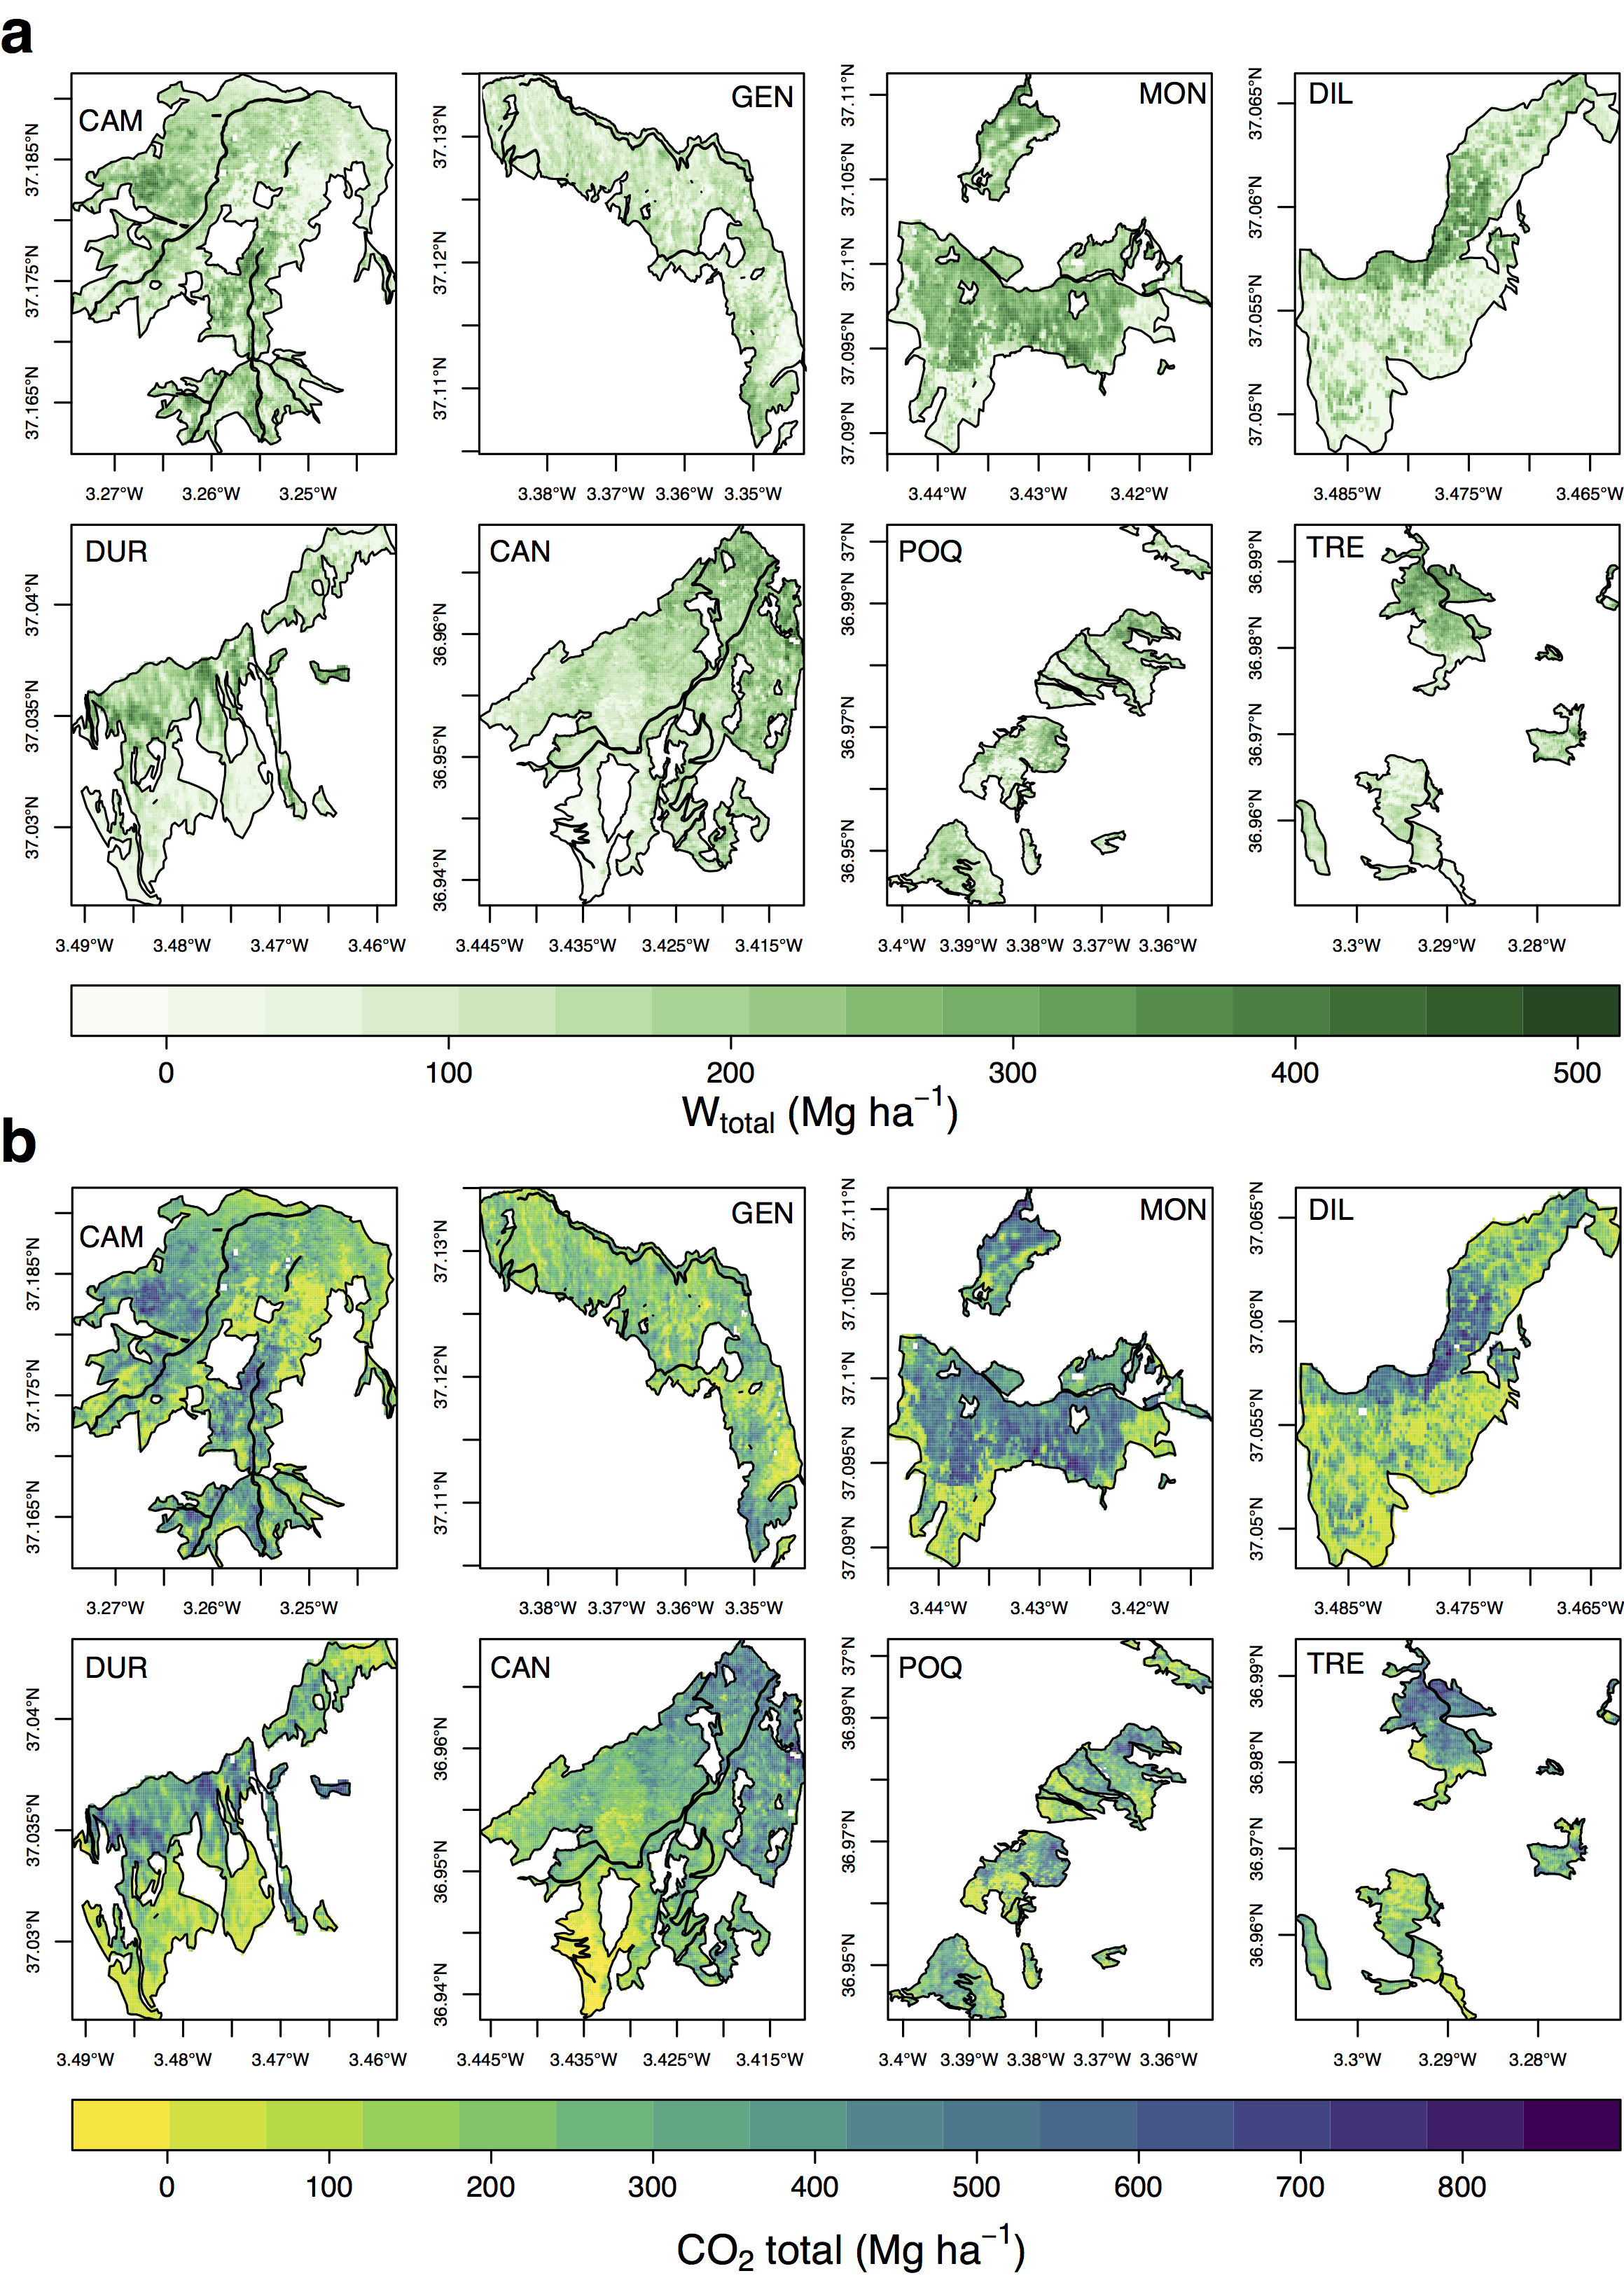
\includegraphics[width=\textwidth]{img/carbon/carbon-mapas-wt-ct.jpg}
    \caption{Total biomass (W~total~) (\textbf{a}) and Potential Carbon sequestration (\textbf{b}) for each of the eight Pyrenean oak populations of Sierra Nevada. Different spatial scales were used for ease of visualization.}
    \label{fig:carbon:mapas-wt}
\end{figure}

The comparison of field-derived measures between oak-cluster populations revealed differences for tree height and DBH, but no for Basal Area and Tree density (Table 3). The oak woodlands of N-cluster showed significantly taller trees with larger DBH than those of the NW and S (Table 3, \figref{fig:carbon:schema}). Lower tree density and higher basal area were observed for N oak-woodlands, but the differences were not significant with the other oak-populations. No differences were found for field-biomass estimation between oak-populations (Table 3).

Significant differences for ALS-estimated biomass were found among oak-clusters (Table 3). The values for the stem fraction (W\textsubscript{stem}) and small branches (W\textsubscript{b2}) biomass fractions were significantly higher for S oak-populations than for those in the N and NW, the latter showing no differences (Table 3). The total biomass (W\textsubscript{total}) was significantly different between oak-population clusters with higher values for southern oak populations (\figref{fig:carbon:schema}). Root biomass (W\textsubscript{root}) and medium branches biomass (W\textsubscript{b2-7}) were significantly higher for northern oak-populations (N) (Table 3; \figref{fig:carbon:schema}).

\begin{figure}
    \centering
    \includegraphics[width=\textwidth]{img/carbon/carbon-esquema-compara2.jpg}
    \caption{Comparison of stand features and ALS-estimated biomass fractions between oak-population clusters of \Qpy woodlands in Sierra Nevada. The distribution of oak-cluster are shown upper-right. Different letters indicate statistically significant differences between oak-population clusters (Dunn's test, p \textless 0.05) after Kruskal-Wallis test.}
    \label{fig:carbon:schema}
\end{figure}

\subsection{Predictions of Stand Biomass}\label{sec:carbon:results-prediction}
The best GLM models selected for total (W\textsubscript{total}), stem (W\textsubscript{stem}) and root (W\textsubscript{root}) biomass explained 70.3\%, 67.3\% and 63.1\% of variance respectively (Tables 4 and A3). The elevation and the shannon structural diversity index showed positive effects on estimated biomass (Table 4; \figref{fig:carbon:glm}). Tree density negatively affected the estimated total biomass. The interaction between tree density and the shannon structural diversity index was significantly (Table 4), indicating that the total biomass increased with the increase structural diversity at lowest and medium tree densities, but decreased at high values of tree density (\figref{fig:carbon:glm}).

\begin{figure}
    \centering
    \includegraphics[width=\textwidth]{img/carbon/carbon-glm-effects.jpg}
    \caption{Predicted effects of the (\textbf{a}) elevation (meters), (\textbf{a}) tree density (trees ha\textsuperscript{-1}), (\textbf{c}) shannon structural diversity index, and (\textbf{d}) tree density x shannon structural diversity index, on the total biomass (W~total~; Mg \textsuperscript{-1}).}
    \label{fig:carbon:glm}
\end{figure}


\subsection{Temporal evolution of Biomass in \Qp stands}\label{sec:carbon:results-temporal}
A general pattern of increase in aboveground tree biomass was observed for most analyzed plots (Table 5), with a total increase of 19 172 Mg ha\textsuperscript{-1} between the two national forest inventories. About 89 \% of the plots showed an increase in aboveground tree biomass, with an average of 11.46 Mg ha\textsuperscript{-1} (Table 5). This general pattern was also observed for plots located in Sierra Nevada (Figure A1).

\section{Discussion}\label{sec:carbon:discussion}
\section{Carbon sequestration by Sierra Nevada oak woodlands.}\label{sec:carbon:discussion-sn}

Total estimated biomass values in Sierra Nevada oak woodlands ranged from 147.27 -- 157.13 Mg ha\textsuperscript{-1} (Table 3), with aboveground biomass (sum of W\textsubscript{stem}, W\textsubscript{b7} and W\textsubscript{b2-7} fractions) ranging from 104.69 - 111.71 Mg ha\textsuperscript{-1}. Our results are consistent with the mean aboveground biomass density cited by the IPCC guidelines as the default value for temperate mountain systems (130 (20 - 600) Mg ha\textsuperscript{-1}) in Europe \autocite{IPCC2006ForestLand}. Using data from the Spanish Third National Forest Inventory, \autocite{Vayredaetal2012SpatialPatterns} reported an average value for stand C stock of 45 Mg ha\textsuperscript{-1} along the distribution of \Qp in the Iberian Peninsula. Those values were lower than the estimated carbon stock (above- and below-ground) in our study which ranged from 69.95 - 74.63 Mg ha\textsuperscript{-1} (Table 3). At a more regional scale, our results showed higher values than those found in the central range of the species distribution, where aboveground biomass varied between 63.8 - 98 Mg ha\textsuperscript{-1} \autocite{GallardoLanchoGonzalezHernandez2004SequestrationCarbon}. Estimates of dioxide carbon sequestration for \Qp pure stands (122.19 - 152.82 Mg ha\textsuperscript{-1}) located in the Central Mountain Range (Spain) \autocite{Canellasetal2008SilvicultureCarbon,Canellasetal2017CarbonSequestration} were also lower than our results (256.72 - 273.91) (Table 3). Despite the potential differences derived from the carbon estimation method (\emph{i.e.} LIDAR estimation \emph{versus} field-ground based estimation; biomass expansion factors), several factors could explain the differences found in our results with respect to the values reported for other studies. First, it is generally accepted that there is an age‐related decline in stand biomass accumulation \autocite[ and references therein]{Xuetal2012AgerelatedDecline} with the productivity of old-growth forests being usually lower than younger forests \autocite{Kutschetal2009EcophysiologicalCharacteristics}. Oak woodlands of Sierra Nevada are composed of relatively young trees \autocite{GeaIzquierdoCanellas2014LocalClimate,PerezLuqueetal2020LanduseLegacies,RubioCuadradoetal2018AbioticFactors} in comparison with other woodlands of the species along their distribution area \autocite{GeaIzquierdoCanellas2014LocalClimate}. The strong anthropic perturbations in these oak has conditioned their structure. For instance, some of the oak woodlands were massively cut down during Spanish Civil post-war period for use as wood gas for vehicles \autocite[\emph{e.g.} MON population;][]{Prieto1975BosquesSierra}, or for use in intense mining activities \autocite[\emph{e.g.} GEN population;][]{PerezLuqueetal2020LanduseLegacies}. Therefore, we can consider that many of the oak woodlands of Sierra Nevada oaks are relatively young, which might explain the high potential for C accumulation obtained in our study, since it has been shown that forest created as a result of drastic land-use changes exhibited faster growing rates, and therefore higher potential C accumulation, than pre-existing forests \autocite{VilaCabreraetal2017NewForests}. Differences in carbon stock between young oak coppices and mature forests were reported for other Quercus species \autocite{Bruckmanetal2011CarbonPools,Cotillasetal2016AbovegroundBelowground}. Therefore, it is likely that the high total ecosystem C values obtained in our area of study could be partly explained by the stands age-development stage \autocite{Makinecietal2015EcosystemCarbon}. Secondly, the water availability is generally the most limiting factor driving radial growth of Q. pyrenaica along its distribution range in the Iberian Peninsula \autocite{GeaIzquierdoCanellas2014LocalClimate}. In Sierra Nevada, northern and northwestern oak populations are located in valley bottoms with high values of relative humidity; and southern ones get the extra supply of water from moist air from the Mediterranean sea. Therefore water availability does not seem to be strongly limiting the oak-growth in this mountain region. In fact, in the last decades positive trends have been observed for greenness and secondary growth of oak woodlands in Sierra Nevada \autocite{GeaIzquierdoCanellas2014LocalClimate,PerezLuqueetal2020LanduseLegacies,RubioCuadradoetal2018AbioticFactors} suggesting that this mountain range could act as an ecological refugee for this species. Thus those positive growth trends could explain the high values of carbon sequestration obtained in our study.

\subsection{Factors explaining biomass in the oak woodlands}\label{sec:carbon:discussion-factors}
Regarding the factors explaining biomass, we found a positive effect of the structural richness on total biomass, and therefore on C stock (Figure 5). Our results are consistent with general patterns obtained for tree species in Iberian Peninsula \autocite{Vayredaetal2012SpatialPatterns}. In structural-heterogeneous stands, trees occupy different horizontal and vertical layers, thus they can maximize the resources, e.g.~light \autocite{Forrester2014StandlevelLight}, whereas homogeneous stand structure may reduce complementary effects \autocite{Goncalves2018EffectsForest,Vayredaetal2012SpatialPatterns}. Being surrounded by size-diverse neighbours allows trees to fill the available canopy space around them and hence capture more light \autocite{Forrester2014StandlevelLight,Vanhellemontetal2018SpeciesStructural}. Our results show that the higher the tree density, the lower the total biomass (Figure 5).
Previous work on forests located on NW of Spain, reported tree stand density as one of the main factors affecting potential biomass production and carbon sequestration \autocite{CastanoSantamariaetal2013PotentialGround}. Tree growth of \Qp is inversely influenced by competition \autocite{Canellasetal2004GrowthResponse,FernandezdeUnaetal2015StandCompetition,FernandezdeUnaetal2016DisentanglingEffect}. Thus, trees respond to reduced competition through the structural shifts such as increased radial growth \autocite{Canellasetal2004GrowthResponse,FernandezdeUnaetal2016DisentanglingEffect}, and therefore a potential increase in biomass. We also found an interaction effect between the tree-density and stand structure diversity (Figure 5) which suggests that at high tree-densities resources are not maximized, even if structural diversity exists.
Despite the importance of the water availability in the growth of \Qp \autocite{GeaIzquierdoCanellas2014LocalClimate,MorenoFernandezetal2020InfluenceClimate}, none of the best models selected for Wtotal, Ws or Wr, included the topographic wetness index (Table A3). This would seem suggest that the water requirement of this species in this mountain is met by the location of the oak populations within Sierra Nevada, and therefore would reinforce the role of this mountain region as an ecological refugee for this species.

\subection{Biomass differences within oak woodlands}\label{sec:carbon:discussion-differences}

We found that oak woodlands of the Northern cluster showed stands with taller and greater trees (Table 3), and also high values of biomass (Figures 3 and 4). It could be related with lower intensity of anthropogenic disturbances in comparison with the other oak woodlands, mainly because the northern oak woodlands had greater protection during the second half of the last century \autocite{JimenezOlivencia1991PaisajesSierra}, and currently also have the highest level of legal protection within the protected area \autocite{Anonymous2011Decreto238}. The less anthropogenic disturbances have resulted in well-conserved forests with a greater species diversity \autocite{PerezLuqueetal2021EcologicalDiversity}, and also an stable stand structure with high values of biomass (Figures 3 and 4). For other species of \emph{Quercus} it has been observed that forests with less disturbance have a higher potential for storage of carbon \autocite{BalboaMuriasetal2006CarbonNutrient,Cotillasetal2016AbovegroundBelowground,Stojanovicetal2017ForecastingTree}.

Our results also highlighted how differences in stand structure conditioned stand tree biomass (Table 4, Figure 5). High dense stands, i.e.~northwestern oak populations, showed lower total biomass than less dense stands (northern or southern oak populations) (Figure 4). High stand density increase tree competition, limiting stand growth which provokes loss of vitality and reduction in acorn production \autocite{Bravoetal2008SelviculturaMontes,Piqueetal2018Spain}, and according to our results, the higher the tree density the lower the capacity of these forests to act as carbon sinks (Figures 4, 5). In addition, an accumulation of biomass, coupled with a loss of structural diversity (Figure 5), would increase the risk of forest fires due to the large amount of biomass \autocite{Canellasetal2004GrowthResponse,PiqueVericat2015EvolutionPerspectives,Serradaetal1992CoppiceSystem}

\subsection{Trends of carbon sequestration by oak woodlands}\label{sec:carbon:discussion-trends}
We observed an increase in aboveground tree biomass between the two inventories for plots located in oak woodlands (Table 5, Figure A1). Recent studies have reported a positive trend for primary production and for secondary growth in oak woodlands in Sierra Nevada \autocite{AlcarazSeguraetal2016ChangesVegetation,Dionisioetal2012SatelliteBasedMonitoring,PerezLuqueetal2015OntologicalSystem,PerezLuqueetal2020LanduseLegacies}. In addition, an increase in the area occupied by oak forests \autocite{CamachoOlmedoetal2002TransformacionPaisaje} as well as the densification of existing forest have been found \autocite{JimenezOlivenciaetal2015MedioSiglo}. All these results indicated that this ecosystem service, \emph{i.e.} carbon sequestration, have suffered an increase in the last decades in our study area. Land-use changes have extensively affected C storage of terrestrial ecosystems for several areas of south Europe \autocite{MunozRojasetal2011ChangesLand,MunozRojasetal2015ImpactLand}. Abandonment of traditional activities and rural exodus are the main drivers explaining the densification and expansion of forests particularly in mountainous regions such as Sierra Nevada \autocite{JimenezOlivenciaetal2015MedioSiglo,MacDonaldetal2000AgriculturalAbandonment}. Considering the positive trend observed for the increase in biomass, and the lack of direct human-drive disturbances as these forests are in a protected area, it would expect a positive trend in forest carbon stock, such as has been recorded in many forests in the Mediterranean region in the last decades \autocite{FAOPlanBleu2018StateMediterranean}. It also agrees with the predictions under different scenarios forecasting a forest growth in the next decades \autocite{Aparicioetal2015ClimateChange}. However, it should be taken with caution, since some early signs of saturation of forests as a carbon sink are being documented in Europe \autocite{Nabuursetal2013FirstSigns}.

\section{Management implications}\label{sec:carbon:discussion-management}

Several studies indicated that reductions of tree-density on oak coppices forests, by moderate thinning, causes an increase in the tree growth and biomass for \Qp woodlands \autocite{Aldeaetal2017ThinningEnhances,Aldeaetal2017EfectoClaras,MorenoFernandezetal2020InfluenceClimate,Canellasetal2004GrowthResponse}, and also for other \emph{Quercus} species \autocites[\emph{e.g.}][]{Cotillasetal2009GrowthResponse,FernandezdeUnaetal2015StandCompetition}. This reduction in the stand density could increase the carbon sequestration of the woodland by a higher structural diversity which maximized the use of resources \autocite{CastanoSantamariaetal2013PotentialGround}. Esta reducción de la densidad, además implica una menor cantidad de biomasa de pequeño tamaño, mejorando las condición fuegos 
% !TEX root = ../my-thesis.tex
%
%\selectlanguage{english}  
\chapter{Land-use legacies and climate change as a double challenge to oak forest resilience: mismatches of geographical and ecological rear edges}\label{sec:dendro}

\newpage

\paragraph{Abstract} \mbox{} \\
Global change challenges ecosystems in xeric locations transformed by intensive human use. Resilience to drought of relict Mediterranean \emph{Quercus pyrenaica} populations in the southern Iberian Peninsula was analyzed in relation to historical records of land use, combining dendroecological growth of adult trees and greenness (EVI) as proxies for secondary and primary growth. The growth trends reflected a strong influence of old land-use legacies (\emph{e.g}. firewood removal) in the current forest structure. Trees were highly sensitive to moisture availability, but both primary growth and secondary growth expressed high resilience to drought events over the short and the long term. Resilience and the tree growth response to climate followed a water-stress gradient. A positive growth trend since the late 1970s was particularly evident in mesic (colder and wetter) high-elevation stands, but absent in the most xeric (warmer and drier) stands. The high values of resilience observed suggest that the studied \emph{Q. pyrenaica} populations are located in a geographical but not a climatic or ecological rear edge. Resilience of oak stands to drought events was not spatially homogeneous across the mountain range, due to differences in ecological conditions and/or past management legacies. This is particularly relevant for rear-edge populations where topographic and biophysical variability can facilitate the existence of refugia.

\newpage

\section{Introduction}\label{sec:dendro:Intro}

The response of species to changing environments (\emph{e.g.} distributional shifts) can be determined largely by population responses at range margins \autocite{HampePetit2005ConservingBiodiversity}. Peripheral populations are usually considered more vulnerable compared with populations at the center of a species' range {[}\emph{i.e.} center-periphery hypothesis; \textcite{SagarinGaines2002AbundantCentre}; \textcite{Pirononetal2017GeographicVariation}{]}. Geographically marginal populations have often been assumed to represent ecologically marginal populations. This means lower performance, higher vulnerability, and thus higher risk of extinction than for populations at the core of the species' range \autocite{Rehmetal2015LosingYour,Pirononetal2017GeographicVariation,VilaCabreraetal2019RefiningPredictions}. Nonetheless, recent reviews report that species- and population-specific responses do not always support this hypothesis \autocite{Sextonetal2009EvolutionEcology,Abelietal2014EffectsMarginality,Oldfatheretal2020RangeEdges}. This is partly because a rear-edge is a multidimensional concept including an ecological (\emph{i.e.} climatic and edaphic), a geographical, and a genetic component \autocite{VilaCabreraetal2019RefiningPredictions}, but also an anthropogenic dimension (\emph{i.e.} land-use). In this respect, to fully understand changes in distribution and abundance of species as a consequence of global change, it is crucial to identify and understand mismatches between the geographical and the ecological rear edges \autocite{VilaCabreraJump2019GreaterGrowth}.

Limits of species distribution are strongly determined by climatic factors and biotic interactions \autocite{Gaston2009GeographicRange,Sextonetal2009EvolutionEcology}. Climate change is expected to cause major shifts in the distribution and abundance of plant communities, and signs already indicate that more intense and longer droughts are altering forest dynamics \autocite{Allenetal2010GlobalOverview}. Drought frequency and severity have increased in recent decades, with a trend towards drier summers, particularly for Southern Europe \autocite{VicenteSerranoetal2014EvidenceIncreasing,Staggeetal2017ObservedDrought}. In this climatic-change context, population loss and range retractions are expected in boreal, temperate, and Mediterranean species at the lowest latitudes and elevations, as well as in drought-prone areas of a species' distribution, \emph{i.e.} the rear edge. The rear-edge populations are likely to be more sensitive to minor climatic and microtopographic variations and therefore the effects of droughts are expected to be particularly noteworthy \autocite{HampePetit2005ConservingBiodiversity,VilaCabreraetal2019RefiningPredictions}.

It is often overlooked that human activity constitutes a driver of change as powerful or even more powerful as natural drivers, \emph{i.e.} natural variation in climate, particularly for regions with long land-use history such as the Mediterranean Region \autocites[\emph{e.g.}][]{NavarroGonzalezetal2013WeightLanduse,DoblasMirandaetal2017ReviewCombination}. In these areas, the susceptibility and response of ecosystems to climate change are conditioned by legacies of historical land-use activity \autocites[\emph{e.g.}][]{Munteanuetal2015Legacies19th,Mausolfetal2018LegacyEffects}. The past land-use legacies interact with recent human-caused climate disturbances and may confound their interpretation \autocite{Fosteretal2003ImportanceLanduse}. For example, recent works showed that a quarter of current forests in the Iberian Peninsula, are growing on former agricultural and grazing land abandoned after the 1950s \autocite{VilaCabreraetal2017NewForests}. Consequently, anthropogenic habitat modification and its legacies represent a critical dimension of marginality as they may intensify, confound or delay climate-driven population decline at rear edges \autocite{VilaCabreraJump2019GreaterGrowth,SanchezdeDiosetal2020FagusSylvatica}. In this context, our work seeks to identify the impacts and responses to natural (\emph{e.g.} severe drought) and human disturbances (\emph{e.g.} logging) on oak forests at their southern geographical range. A historical perspective should help us to interpret the responses of ecosystems to disturbances \autocite{Fosteretal2003ImportanceLanduse}, particularly regarding marginal rear-edge populations \autocite{VilaCabreraetal2019RefiningPredictions}.

The assessment of resilience to climate and human disturbances provides critical information concerning the capacity of forests to maintain their structure and render valuable ecosystem services. Resilience is the capacity of an ecosystem to persist and maintain its state and functions in the face of disturbance \autocite{Holling1973ResilienceStability,Hodgsonetal2015WhatYou}. \textcite{Lloretetal2011ComponentsTree} proposed an approach, which decomposes resilience into three components: resistance to drought, recovery after drought and resilience. This resilience is determined by the forest's ability to mitigate the disturbance (resistance) and the capacity to recover from the impact (recovery) \autocite{IngrischBahn2018ComparableQuantification}. This conceptual approach has recently become widely used to assess forest resilience, because it allows a simple, yet highly efficient assessment of short-term responses of trees to drought. Nevertheless, not exempt from criticism, this approach needs to be applied carefully to avoid potential bias at different levels \autocite{Schwarzetal2020QuantifyingGrowth}. In this sense we assessed forest resilience both over the short-term to several recent extreme drought episodes, as well as over the long-term to climate change (\emph{i.e.} warming on the last few decades), using two different proxies to characterize resilience. Dendroecological estimates of growth (\emph{i.e.} tree-ring width) are commonly used proxies to characterize tree vitality and have commonly been used to study growth changes in response to drought at the individual tree level \autocite{Fritts1976TreeRings,Dobbertin2005TreeGrowth}. Remote sensing can be used to analyze the impact of drought on ecosystems at the stand level \autocite[\emph{e.g.}][]{Zhangetal2013MonitoringEstimating}. Tree-ring records complement remote-sensing data with a longer time scale. Tree rings can reflect tree-growth anomalies induced by climate or other disturbance over decades to centuries \autocite{Babstetal2017ImprovedTreering} and provide an accurate measure of growth responses to droughts \autocite{Bhuyanetal2017DifferentResponses}. The combination of remote sensing and dendroecology has been used to assess the effects of droughts on vegetation along ecological gradients \autocites[\emph{e.g.}][]{VicenteSerranoetal2013ResponseVegetation,Coulthardetal2017TreeGrowth}, and also to evaluate growth resilience to drought in several tree species \autocites[\emph{e.g.}][]{Gazoletal2018ForestResilience,PenaGallardoetal2018DroughtSensitiveness}.

In the present study, we assess resilience of \emph{Quercus pyrenaica} Willd. (Pyrenean oak) from southern relict forests at the rear edge of the species distribution, where species performance is considered to be threatened by climate change \autocite{GeaIzquierdoetal2013GrowthProjections,GeaIzquierdoetal2017RiskyFuture}. For this, we combined remote-sensing information and dendroecological methods to evaluate the impact of drought both on canopy greenness (as a proxy for primary growth) and radial tree growth (as a proxy for secondary growth). For the analysis of forest resilience to climate, we took into account the land-use history of these transformed forests, thoroughly reviewing historical documents to reconstruct forest history at the study sites, and analyzing how anthropogenic drivers have shaped the current forest structure. Based on this analysis, we developed a rationale that integrates the ecological and anthropogenic components of marginality to determine the regional and local scale mechanisms shaping the probability of persistence (or extinction) of rear-edge oak populations. Our main hypothesis is that range edge stands will show low resilience to extreme droughts, but that the vulnerability to drought will be reduced quickly across a fine-scale topographic gradient of decreasing aridity. To test this hypothesis, we: (\emph{i}) quantified how recent extreme drought events influenced primary and secondary growth of \emph{Q. pyrenaica} forests at their present geographical rear edge; (\emph{ii}) analyzed the long-term resilience of these forests to extreme drought events, using time-series of radial growth; (\emph{iii}) reviewed historical documents to reconstruct forest-management history and to infer how it impacted tree growth and stand dynamics over time; (\emph{iv}) and examined differences in the resilience metrics between populations under contrasting ecological conditions (\emph{i.e.} xeric \emph{vs.} mesic) along environmental gradients within the rear edge in order to detect vulnerability to climate change at the small spatial scale.

\begin{sidewaystable} 
\caption{Characteristics of sampled plot. Lat = latitude; Long = longitude. Dbh and height of all trees, Basal Area (BA), Density and SRD (size ratio proportional to distance) are computed for all trees within a 10-m radius of focal trees (see Materials and methods). Temp.: annual average of mean monthly minimum and maximum temperatures. Values shown here correspond to site averages. Standard deviations are shown in parentheses. Different letters indicate statistically significant differences between sites (Kruskal-Wallis test followed by Dunn’s test, \emph{p<0.05}). Stands were monospecific, hence all results correspond to oak data.}\label{tab:sampledPlots}
\begin{adjustbox}{width=\linewidth}
\begin{threeparttable}
\begin{tabular}{p{1cm}p{1.2cm}p{1.2cm}p{2.3cm}p{1.3cm}p{1cm}p{1.3cm}p{2cm}p{1.4cm}p{1.3cm}p{1.6cm}p{1.8cm}p{1.8cm}p{1.9cm}p{2cm}p{1.8cm}}
 &  &  &  &  &  &  & \multicolumn{4}{l}{Cored trees} & \multicolumn{5}{l}{Stand competition} \\ \cline{8-16}
\textbf{Site} & \textbf{Lat (º)} & \textbf{Long (º)} & \textbf{Elevation (m)} & \textbf{Slope (º)} & \textbf{Prec. (mm)} & \textbf{Temp. (ºC)} & \textbf{\#trees (\#cores)} & \textbf{Dbh (cm)} & \textbf{Height (m)} & \textbf{Age (years)} & \textbf{Dbh all (cm)} & \textbf{Height all (m)} & \textbf{BA (m\textsuperscript{2}ha\textsuperscript{-1})} & \textbf{Density (trees ha\textsuperscript{-1})} & \textbf{SDR} \\ \hline
CA-High & 36.97 & -3.42 & 1846 - 1884 & 12.11 (3.28) & 731 & 3.4-13.8 & 15 (30) & 69.8 (20.5) a & 15.4 (1.8) a & 161.0 (32.2) a & 34.1 (24.3) a & 10.8 (4.4) a & 39.13 (24.31) a & 348.0 (147.1) a & 0.91 (0.63) a \\
CA-Low & 36.96 & -3.42 & 1691 - 1751 & 12.86 (2.98) & 658 & 4.7-15.6 & 15 (30) & 45.9 (8.6) a & 12.6 (1.6) b & 148.5 (16.5) a & 21.7 (14.4) b & 9.0 (2.8) b & 18.02 (7.11) ab & 409.6 (226.0) a & 0.89 (0.44) a \\
SJ & 37.13 & -3.37 & 1322 - 1474 & 27.33 (5.59) & 555 & 4.9-16.35 & 20 (48) & 31.9 (3.7) b & 11.8 (2.3) b & 72.6 (11.1) b & 20.6 (8.1) b & 9.7 (3.6) ab & 11.64 (5.47) b & 339.0 (130.3) a & 1.11 (0.52) a \\ \hline
\end{tabular}%
\end{threeparttable}
\end{adjustbox}
\end{sidewaystable}

\section{Material and Methods}\label{sec:dendro:MatMet}
\subsection{Tree species and study site}\label{sec:dendro:StudyArea}
\emph{Quercus pyrenaica} forests extend throughout south-western France and the Iberian Peninsula, reaching their southern limit in mountain areas of northern Morocco \autocite{Franco1990Quercus}. In the Iberian Peninsula, these forests occupy siliceous soils under meso-supramediterranean and mesotemperate areas and subhumid, humid, and hyperhumid ombroclimate. Pyrenean oak is a deciduous species that requires over 650 mm of annual precipitation and some summer precipitation. As a submediterranean species, it has lower drought tolerance than evergreen Mediterranean taxa \autocite{delRioetal2007BioclimaticAnalysis}.

\begin{figure}
\centering
\includegraphics[width=\textwidth]{img/dendro/dendro-mapa.jpg} \caption{Distribution of \textit{Quercus pyrenaica} forests in the Iberian Peninsula \textbf{a} and in Sierra Nevada mountain range \textbf{b}. Different colors indicate oak-population clusters identified in Sierra Nevada \autocite{PerezLuque2015}. For each population, a grid with the MODIS pixels is shown (see Material and methods). Detailed location of the dendroecological sampling sites: northern (San Juan, SJ) \textbf{c}, and southern ones (Cáñar: CA-Low and CA-High) \textbf{d}. Color orthophotography of 2009 from Regional Ministry of the Environment.}
\label{fig:map}
\end{figure}

The forests of this species reach their southernmost European limit in Andalusian mountains such as Sierra Nevada (37°N, 3°W), a high-mountain range with elevations of up to 3482 m \emph{a.s.l.}. The climate is Mediterranean, characterized by cold winters and hot summers, with pronounced summer drought and increasing aridity with decreasing altitude, and marked variability in annual rainfall according to elevation and aspect. Sierra Nevada is considered a glacial refuge for deciduous \emph{Quercus} species \autocite{Olaldeetal2002WhiteOaks}. Eight Pyrenean oak patches (2400 ha) have been identified in this mountain range (\figref{fig:map}), from 1100 to 2000 m \emph{a.s.l.} and often associated with major river valleys. Today, \emph{Quercus pyrenaica} woodlands in this mountain region represent a rear edge of their habitat distribution \autocite{HampePetit2005ConservingBiodiversity}. They are the richest forest formation in vascular plant species of Sierra Nevada, containing several endemic and endangered plant species \autocite{Loriteetal2008PhytosociologicalReview}. They also harbor high levels of intraspecific genetic diversity \autocite{ValbuenaCarabanaGil2013GeneticResilience}. These relict forests have undergone intensive human use throughout history \autocite{CamachoOlmedoetal2002DinamicaEvolutiva}. Furthermore, the conservation status of this species for southern Spain is considered ``Vulnerable'' and it is expected to suffer from climate change, potentially reducing its suitable habitats in the near future \autocite{GeaIzquierdoetal2013GrowthProjections,GeaIzquierdoetal2017RiskyFuture}.

\subsection{Climatic data and drought episodes}\label{sec:dendro:Climate}
The Iberian Peninsula underwent several extreme drought episodes in the last three decades \autocite[\emph{e.g.} 1995, 1999, 2005, 2012][]{VicenteSerranoetal2014EvidenceIncreasing}. The 2005 and 2012 drought events have been documented as being among the worst in recent decades for the southern Iberian Peninsula \autocite{Pascoaetal2017DroughtTrends}, appearing as extreme drought in our climatic data (\figref{fig:dendro:s1climate}; \tabref{tab:dendro:droughts}). We focused on these two drought events because they were included in the period having remote-sensing information of high spatial resolution (MODIS started on 2000; see below). Nevertheless, for radial growth-time series, a greater number of older drought events were also analyzed to contextualize the results for 2005 and 2012 and to evaluate forest resilience to drought over a longer term (see \tabref{tab:dendro:droughts}). A drought event was identified using the SPEI (Standardized Precipitation-Evapotranspiration Index) \autocite{VicenteSerranoetal2010MultiscalarDrought} (SPEI 12-months scale), following a procedure similar to the one proposed by \textcite{Spinonietal2015EuropeanDrought}. We used 0.5º grid cells covering Sierra Nevada taken from the Global SPEI Database (\url{http://spei.csic.es/database.html}). A severe drought event starts when SPEI falls below the threshold of -1.28 \autocite{Spinonietal2018WillDrought,Pascoaetal2017DroughtTrends}. A drought event is considered only when SPEI values fall below that threshold for at least two consecutive months. For each drought event, we computed: the \emph{duration} as the number of consecutive months with the SPEI lower than a certain threshold; the \emph{severity} as the sum of the absolute SPEI values during the drought event; the \emph{intensity} and the \emph{Lowest SPEI} refer to the mean and lowest value of SPEI respectively during the drought event.

To explore the relationships between climatic variables and tree-growth variables we used climate data obtained from the European Daily High-Resolution Observational Gridded Dataset (E-OBS v16) \autocite{Haylocketal2008EuropeanDaily}. Monthly precipitation and minimum and maximum temperatures had a 0.25 x 0.25 º resolution for the 1950-2016 period. Grid cells were selected to cover each sampled site. The SPEI 6-months scale index was used to characterize the drought conditions for the period 1961-2014.

\subsection{Greenness data to assess ecosystem resilience}\label{sec:dendroEVI}
Vegetation greenness of \emph{Quercus pyrenaica} was characterized by means of the \emph{Enhanced Vegetation Index} (EVI), derived from MOD13Q1 product of the MODIS sensor. EVI data consists of 16-day maximum value composite images (23 per year) of the EVI value with a spatial resolution of 250 m x 250 m. MODIS EVI data were compiled for the period 2000 - 2016. We selected the pixels covering the distribution of \emph{Quercus pyrenaica} forests in Sierra Nevada (\emph{n} = 928 pixels). Any values affected by clouds, snow, shadows or high content aerosols, were filtered out following recommendations for mountain regions \autocite{ReyesDiezetal2015ImplicacionesFiltrado}.

The mean Annual EVI (\(EVI_{mean}\)) as a surrogate of mean annual primary production was computed for each pixel for the period 2000 - 2016. The EVI standardized anomaly (\(EVI_{sa}\)) was computed pixel-by-pixel, in order to minimize bias in the evaluation of anomalies and to provide more information concerning their magnitude \autocite{Samantaetal2012InterpretationVariations}. For each pixel, an annual EVI value was calculated by averaging EVI valid values. Then, the standardized anomaly was computed as: \[\mathrm{EVI_{sa,\mathit{i}}}= (\mathrm{EVI_{mean,\mathit{i}}-EVI_{mean,ref}})\Big/\sigma_{\mathrm{ref}}\]
where \(\mathrm{EVI_{sa,\mathit{i}}}\) is the EVI standardized anomaly for year \(i\); \(\mathrm{EVI_{mean,\mathit{i}}}\) the annual mean value of EVI for year \(i\); \(\mathrm{EVI_{mean,ref}}\) the average of the annual EVI values for the period of reference 2000-2016 (all except year \(i\)); and \(\sigma_{\mathrm{ref}}\) the standard deviation for the reference period. Each pixel was categorized according the EVI standardized anomalies as ``greening'' (\(EVI_{sa} > 1\)), ``browning'' (\(EVI_{sa} <- 1\)) or ``no-changes'' (\(-1 > EVI_{sa} > 1\))\autocite{Samantaetal2012InterpretationVariations}.

Rather than other vegetation indices such as the NDVI, \(EVI_{mean}\) was chosen because it is highly stable under the use of any filter \autocite{ReyesDiezetal2015ImplicacionesFiltrado} and because it showed highly significant correlations with annual (\(r\)= 0.81) and seasonal EVI values (\(r_{spring}\)= 0.76 and \(r_{summer}\)= 0.88).

\subsection{Field sampling and dendroecological methods to assess individual tree resilience}\label{sec:dendro:Field}
Trees were sampled during the autumn of 2016 at two locations in contrasting N-S slopes of Sierra Nevada: San Juan (SJ), a xeric site located at the northern aspect (around 1400 m); and Cáñar (CA), a wetter site located at the southern aspect (\figref{fig:map}; \tabref{tab:sampledPlots}). For the southern site, two elevations were sampled: CA-Low (around 1700 m) and CA-High (around 1860 m), constituting the current low-elevational limit for the species (CA-Low) and the maximum altitude currently reached by trees (CA-High), respectively, in the site sampled. Despite the proximity of these two elevations (less than a 200-m difference) the stands differ markedly in their structure and characteristics (\tabref{tab:sampledPlots}). The three sampling sites followed a moisture gradient: SJ \textless{} CA-Low \textless{} Ca-High (\tabref{tab:sampledPlots}). All the sites were oak monospecific and representative of the population clusters identified for the species in this mountain range \autocite{PerezLuqueetal2015DatasetMIGRAME}. At each site, between 15 and 20 trees from either the single dominant-codominant layer in CA or the open canopy in SJ were randomly sampled. Two cores of 5 mm in diameter were taken from each tree at breast height (1.3 m) using an increment borer. Diameter at breast height (DBH) and total height were measured for each tree. In addition, stand competition affecting target trees was assessed by recording distance, azimuth, DBH, species, and total height of all neighboring living trees with DBH \textgreater{} 7.5 cm within a circular plot with a 10-m radius. Several competition indices were calculated: the distance independent indices \emph{density} (\(\mathrm{trees \cdot ha^{-1}}\)), and \emph{basal area} (BA, \(\mathrm{m^{2} \cdot ha^{-1}}\)); and the distance dependent index size ratio proportional to distance \autocite[see][ for more details]{GeaIzquierdoCanellas2009AnalysisHolm} as: \[\mathrm{srd} = \sum_{i=1}^{n} (dbh_j / dbh_i) \cdot \left[1/ (dist_{ij} + 1) \right ]\]

Tree cores were air dried, glued onto wooden mounts, and sanded. Annual radial growth (ring width, RW) was determined with a measuring device coupled to a stereomicroscope, for an accuracy of 0.001 mm. Individual ring series were first visually and statistically cross-dated with TSAP software (Rinntech, Heidelberg, Germany), using the statistics Gleichläufigkeit (GLK), t-value and the crossdating index (CDI). Cross-dating validation was finally verified using COFECHA \autocite{Holmes1983ComputerassistedQuality}.

The growth trends were analyzed at different time scales. To study the growth response to the inter-annual variability of climate (short-term response), pre-whitened residual chronologies (RWI) were used. These were calculated from ratios between raw growth measurements and individual cubic splines with a 50\% frequency cutoff at 30 years \autocite{Fritts1976TreeRings}. Tree-ring width series were standardized and detrended using dplR \autocite{Bunn2010StatisticalVisual}. Mean residual site chronologies were established by computing the biweight robust mean of all prewhitened growth indices for the trees of the same site \autocite{Fritts1976TreeRings}. The statistical quality of each chronology was checked via the expressed population signal (EPS). A threshold value of EPS \textgreater{} 0.85 was used to determine the cutoff year of the time span that could be considered reliable.

The long-term growth response was analyzed using basal area increment (hereafter BAI, \(\mathrm{cm^2 \cdot year^{-1}}\)). In theory, BAI represents a more accurate indicator of growth than ring width, because it removes variation in growth attributable to increasing stem circumference after 30-40 years of juvenile growth \autocite{BiondiQeadan2008TheorydrivenApproach}. Raw ring widths and measured DBH were used to compute BAI \autocite{Piovesanetal2008DroughtdrivenGrowth} with the following equation: \[\mathrm{BAI} = \pi(r^2_{t}-r^2_{t-1})\] where \(r\) is the radius of the tree and \(t\) is the year of tree-ring formation. For each individual tree, a mean BAI series was calculated. Then, mean site BAI chronologies were determined by averaging individual tree BAI time series.

\subsection{Disturbance analyses and land-use history review}\label{sec:dendro:Disurbance}
Disturbance chronologies were built using tree-ring width to identify abrupt and sustained increases (release events from competition) or decreases (suppressions) in radial growth \autocite{NowackiAbrams1997RadialgrowthAveraging} as indirect estimates of possible disturbance events (\emph{e.g.} logging, drought-induced neighbor mortality) in the past. Growth changes (GC) were calculated for the individual tree-ring series using a 10-year running window as either positive (PGC) or negative (NGC) growth changes: \[\mathrm{\% GC} = \left[(M1 - M2)\Big/ M2\right] \times 100\] where \(M1\) is the preceding 10-year median and \(M2\) is the subsequent 10-year median \autocite{RubinoMcCarthy2004ComparativeAnalysis}.

Site-disturbance chronologies were constructed by annually averaging the individual disturbance series. To separate growth peaks caused by disturbance events and expressing stand-wise disturbances from those caused by climate, we considered a threshold of 50\% of GC and more than 50\% of the individual trees displaying the same growth changes \autocite[\emph{e.g.}][]{GeaIzquierdoCanellas2014LocalClimate}. In addition, the history of the forest and management of our sampling sites was inferred from a detailed analysis of historical land-use changes. For this, existing historical documents were exhaustively reviewed to compile information on socio-economical activities affecting the forests being studied (\tabref{tab:dendro:reviewusos}). We exhaustively reviewed existing documentary sources: historical documents and maps; detailed mining reports; official information on recent wildfires events and forest-management practices; livestock farming; traditional irrigation channels; and studies concerning the socioeconomic dynamics of forests on Sierra Nevada at different spatio-temporal scales (see \tabref{tab:dendro:reviewusos} for references).

\subsection{Assessing resilience to drought at the forest stand and individual-tree levels}\label{sec:dendro:Resilience}
To evaluate the effects of drought events on ecosystem resilience (using greenness data) and individual tree resilience (using BAI data), we used resilience indices proposed by \textcite{Lloretetal2011ComponentsTree}. The Resistance index estimated as the ratio between performance during and before the disturbance (\(Resistance=Drought/PreDrought\)) quantifies the severity of the impact of the disturbance in the year it occurred. The Recovery index, computed as the ratio between performance after and during disturbance (\(Recovery= PostDrought/Drought\)), represents the ability to recover from disturbance relative to its severity. Finally, the Resilience index (\(Resilience = PostDrought/PreDrought\)) is the capacity to reach pre-disturbance performance levels. The values of these indices were computed for tree growth (BAI) and greenness (EVI mean) during each drought event. The predrought and postdrought values of each target variable (\emph{i.e.} BAI or EVI) were computed as the mean value over a period of three years before and after the drought event, respectively. A period of three years was chosen because we found similar results on comparing periods of two, three, and four years (\figref{fig:dendro:s3correlations}b), and this time period has been used in other studies \autocite[\emph{e.g.}][]{Gazoletal2018ForestResilience}. Resilience metrics for BAI data were additionally computed for the most severe drought events since 1940 (\emph{n} = 8; \tabref{tab:dendro:droughts}) and compared with drought severity.

\begin{figure}
\centering
\includegraphics[width=\textwidth]{img/dendro/dendro-schema.jpg} \caption{Schema of the different metrics \textbf{a} and analyses \textbf{b} used in the manuscript (see Material and methods for details). The severe drought events since 1901 were identified using SPEI-12 and characterized in terms of duration, severity and intensity. Climate impacts on vegetation were assessed for greenness and tree-growth. Non climatic disturbances on vegetation were quantified using growth changes on tree growth (\%GC) and were also related with anthropogenic alterations inferred from review of historical documents. Responses of vegetation to disturbances were explored in the short- and the long-term using resilience metrics and temporal trends respectively for both EVI and BAI. Resilience metrics of BAI were computed for the eight most severe drought events since 1950, and their relationship with drought severity were explored. For the 2005 and 2012 drought events we also compared EVI and BAI resilience metrics among the three \textit{Q. pyrenaica} populations. Numbers (\textit{grey circles}) indicate the study aims to which the analyses are related.}
\label{fig:schemadendro}
\end{figure}

\begin{table}[]
\caption{Characteristics of the mean tree-ring chronologies. Length values in parentheses indicate the number of years replicated with more than five series. \emph{RW} = mean annual ring width (standard deviation in parenthesis). MS = mean sensitivity. AR(1) = mean autocorrelation of raw series. Rbt = mean correlation between series. EPS = mean expressed population signal. EPS and Rbt were calculated for the mean residual chronologies of growth indices.}
\resizebox{\linewidth}{!}{
\begin{tabular}{@{}lllllllllll@{}}
\toprule
Site & First    year & Last    year & Length    (years) & \#    trees & \#    cores & RW    (mm) & MS & AR(1) & Rbt & EPS \\ \midrule
CA-Low & 1836 & 2016 & 181 (164) & 15 & 30 & 1.253 (0.781) & 0.208 & 0.799 & 0.520 & 0.897 \\
CA-High & 1819 & 2016 & 198 (188) & 15 & 30 & 1.500 (0.879) & 0.203 & 0.827 & 0.522 & 0.907 \\
SJ & 1921 & 2016 & 96 (90) & 20 & 48 & 1.725 (1.207) & 0.319 & 0.692 & 0.637 & 0.959 \\ \bottomrule
\end{tabular}}
\label{tab:chronologies}
\end{table}

\subsection{Statistical analysis}\label{sec:dendroStats}
Differences between sites for height, DBH, and competition indices were analyzed using non-parametric Kruskal-Wallis rank sum tests. When significant differences were detected, multiple comparisons were run using the Dunn's-test with Bonferroni adjustment to correct for significance.

The severe drought events since 1901 were identified using SPEI-12. They were characterized in terms of duration, severity and intensity \autocite[see][]{Spinonietal2015EuropeanDrought}. In a first step, the impact of drought in greenness and growth was explored using the \(EVI_{sa}\) and the mean RWI site chronologies (\figref{fig:schemadendro}). Additionally the relationships between climatic variables and tree-growth variables (RWI and BAI site chronologies) were assessed using bootstrapped Pearson's correlations estimated using treeclim \autocite{ZangBiondi2015TreeclimPackage}. The non-climatic disturbance impacts on tree-growth were evaluated using site disturbance chronologies (built using growth changes on tree growth).

Responses of vegetation to disturbances were explored in the short- and the long-term using resilience metrics (resilience, resistance and recovery) and temporal trends respectively for both EVI and BAI (\figref{fig:schemadendro}). Resilience metrics of BAI were computed for the eight most severe drought events since 1950 (including 2005 and 2012), and their relationship with drought severity were explored. Resilience metrics of EVI were computed only for 2005 and 2012 drought events. Temporal trends of \(EVI_{mean}\) (pixel scale) and BAI (mean BAI site chronologies) were examined using non-parametric (Mann-Kendall) and parametric test (Pearson) respectively.

\begin{figure}
\centering
\includegraphics[width=\textwidth]{img/dendro/dendro-evisa.jpg} \caption{EVI standardized anomaly during the period 2000-2016 for northern and southern populations \textbf{a}. Error bars show standard error. See main text for details on EVI calculation. Percentage of pixels showing browning, greening or no changes during the 2005 and 2012 drought events according to EVI standardized anomalies \textbf{b}. See main text for an explanation of greening and browning.}
\label{fig:evisa}
\end{figure}

For each of the three resilience indices studied, we used robust two-way ANOVAs to test for differences between drought events (2005 and 2012) and the oak populations studied (northern and southern exposures). These tests were used because original and log-transformed data did not follow the assumptions of normality or homogeneity of variance \autocite{Wilcox2012IntroductionRobust}. Robust measures of central tendency (M-estimator based on Huber's Psi) were used because they were close to the mean value in all cases \autocite{Wilcox2012IntroductionRobust}. When the robust ANOVA test was run, data were bootstrapped 3000 times and trimmed automatically to control the potential influence of outliers. \emph{Post-hoc} differences were assessed pairwise using a similar bootstrap test. All the robust ANOVA and \emph{post-hoc} tests were carried out using the WRS2 R package \autocite{Mairetal2017WRS2Wilcox}. The level of significance was set to 0.05 and adjusted for multiple comparisons.

\section{Results}\label{sec:dendroResults}
\subsection{Temporal trends in vegetation greenness}\label{sec:dendro:ResultsEVI}

The analysis of temporal trends in greenness showed that 78.9\% of the EVI pixels followed a positive trend for the 2000-2016 period. The lowest values of EVI standardized anomalies for the study period were recorded during the 2005 drought, and the minimum EVI values were expressed in the northern (dry) population (\figref{fig:evisa}a). A ``browning'' episode (\(\mathrm{EVI_{sa}} < -1\)) was found during this drought event, whereas no changes in greenness in response to the 2012 drought were detected (\figref{fig:evisa}b).

\subsection{Analysis of radial-growth trends and disturbances}\label{sec:dendro:ResultsBAI}
The trees of the southern population were older than those from the northern one (\tabref{tab:chronologies}). In addition, trees from the southern population at high elevation were taller and their growth was significantly greater than that of trees from the other two sites. Stand competition measured as plot basal area was greatest in CA-High (\tabref{tab:sampledPlots}, \figref{fig:bai}a). The growth and height of trees from the northern and the low-elevation southern population were similar (\figref{fig:bai}a and S3a). Only trees from the southern sites (\emph{i.e.} the wetter exposure) showed significant positive growth trends since the late 1970s (\figref{fig:bai}a), this trend being far more pronounced for the wetter and colder high elevation site (CA-High).

Drought events reduced radial growth for all sites (\figref{fig:dendro:s2chronos}a). The strongest reduction in radial growth occurred in response to the 1995 drought (the worst drought spell in our climatic record, \tabref{tab:dendro:droughts}) for all sites. Tree-growth reductions in response to drought followed a moisture gradient. Tree-growth reductions in response to the studied drought events were lower in the southern sites (CA-High and CA-Low) than in the northern site (SJ), especially for 2005 and 2012 (\figref{fig:dendro:s2chronos}a). The weakest growth reductions were found in trees from the wettest site (CA-High).

The response of tree growth to water availability was greater than to temperatures. Cumulative precipitation of the hydrological year and seasonal SPEI values (\emph{i.e.} for the Hydrological year, Spring and Summer) were the climatic variables exhibiting the highest (positive) relationship with growth for all populations (\figref{fig:dendro:s6corclimate}a). Nevertheless, there were differences between populations: the positive relationship with SPEI was highest in the more xeric northern population (r \textgreater{} 0.6 \emph{vs.} r \textless{} 0.5; \figref{fig:dendro:s6corclimate}a).

The northern site (SJ) showed two major release events (GC \textgreater{} 50\% occurring in more than 50\% of trees sampled): the first during the 1940s (the most evident) and the second in 1995-2000 (\figref{fig:bai}b). These periods alternated with periods of suppression. By contrast, the two southern sites showed no release events except for CA-High at the beginning of the 1830s and no suppression events in the last 50 years.

\begin{figure}
\centering
\includegraphics[width=\textwidth]{img/dendro/dendro-cronos-bai-gc.jpg}\caption{
Basal Area Increment (BAI) chronologies of \textit{Q. pyrenaica} for northern population (SJ; \textit{red}) and southern ones: low-elevation (CA-Low; \textit{green}) and high-elevation (CA-High, \textit{blue}) sites \textbf{a}. Shading areas correspond to standard error of the mean. Number of series is displayed in the upper plot. Only years replicated with \# series \textgreater{} 5 are shown. Linear trends since 1975 are indicated for all sites (numbers indicate \(r^2\) values; asterisks indicate significant linear trend, p \textless{} 0.001). Comparison of median growth change (\(GC\)) following \textcite{NowackiAbrams1997RadialgrowthAveraging} for \textit{Q. pyrenaica} sites \textbf{b}. Dashed black lines indicate a threshold of 50\% of GC (see Material and methods). Note that y-axes do not correspond in all of the three panels for the sake of clarity. Error bars indicate standard error.}
\label{fig:bai}
\end{figure}

\subsection{Resilience, resistance and recovery to drought events at the stand and individual-tree levels}\label{sec:dendro:ResultsResilience}

Resilience and resistance varied in the same direction whereas recovery varied inversely to resilience and resistance. During the last two drought events, resilience metrics for greenness and tree growth significantly differed between drought events (\tabref{tab:dendro:robustanova}). The 2005 drought event reduced greenness and growth more than that of 2012 (\tabref{tab:dendro:huber}) but the metrics of resilience generally covaried in the same direction during those two drought events. For EVI, resilience and resistance values were significantly higher for 2012, the most severe event, than for 2005 (\tabref{tab:dendro:huber}; \figref{fig:resilience}b); whereas recovery values were higher for 2005 than for the 2012 drought event. For BAI, the resilience, resistance and recovery values were higher for 2012 than for 2005 (\tabref{tab:dendro:huber}, \figref{fig:resilience}c).

The recovery and resistance for greenness and growth varied significantly between sites. Resilience calculated for greenness also differed between sites but not for tree growth (p = 0.534; Table S1). The two southern populations showed lower recovery values than did the northern site both for greenness and tree growth, but resistance and resilience values were significantly higher for the southern site (Table S2).

Resilience metrics of tree-growth for drought events since 1950 (\emph{i.e.} shared period among the three chronologies excluding the juvenile years, \tabref{tab:dendro:droughts}) revealed a positive relationship between drought severity and recovery, significant for all oak populations (\figref{fig:resilience}a). A similar pattern was found for resilience but proved significant only for SJ. Importantly, non-significant patterns resulted when we excluded 1995, except for recovery in SJ (\figref{fig:dendro:s5resilience}). The trees showed the highest value of tree-growth resilience for 1995, the worst drought event in our study area, particularly SJ where our results suggest a major release event also after 1995 (\figref{fig:bai}b).

\section{Discussion}\label{sec:dendro:Discussion}
By using a combined approach of remote-sensing information and dendroecology, we quantified the growth of adult trees and greenness (EVI) as proxies for secondary and primary growth of relict Mediterranean \emph{Quercus pyrenaica} populations in the southern Iberian Peninsula. These relict oak populations, driven by historical land-use, have been resilient to climate change at their present rear edge. However, resistance, resilience, and forest recovery after extreme drought events were strongly influenced by mountain exposure, local environmental conditions, and management legacies. This means that the geographical and the ecological rear edges do not necessarily match and, at a small spatial scale, tree performance can vary markedly along the rear edge under climate change.

\begin{figure}
\centering
\includegraphics[width=\textwidth]{img/dendro/dendro-resiliences.jpg}\caption{
Resilience metrics of tree-growth for eight severe drought events since 1950 (see main text for details) as a function of drought severity \textbf{a}. Points indicate resilience metrics for oak populations: SJ (\textit{red}), CA-High (\textit{blue}) and CA-Low (\textit{green}). Resilience metrics were computed for each population (sample depth > 10) and drought event. Gray lines represent overall relationships for each Resilience metrics. Comparison of the response of  *Q. pyrenaica* forests to drought in terms of resistance, recovery, and resilience of greenness (\textbf{a}) and tree growth (\textbf{c}). For EVI, northern populations (\textit{red circle}) were compared with southern ones (\textit{green circle}). For BAI, the more xeric northern population (San Juan, SJ; \textit{red circle}) was compared with the two southern populations, Cáñar-High (CA-High; \textit{blue circle}) and Cáñar-Low (CA-Low; \textit{green circle}). Different letters indicate significant \textit{post hoc} differences between groups (see Material and methods for details).} 
\label{fig:resilience}
\end{figure}
\hypertarget{sec:dendroHighSensitivity}{%
\subsection{High sensitivity and variability in the oak sensitivity to climate at the rear edge}\label{sec:dendroHighSensitivity}}

Severe drought negatively affects both primary and secondary growth of \emph{Q. pyrenaica} forests. This was expressed by the observed reduction in greenness and tree growth in response to the 2005 and 2012 drought events as well as by radial-growth suppression during extreme drought events \autocite{Corcueraetal2006RadialgrowthWoodanatomical,GeaIzquierdoCanellas2014LocalClimate}. Furthermore, the greatest reduction of tree growth was detected during the 1995 drought, a characteristic negative precipitation anomaly that caused severe and extensive damage in the Mediterranean Iberian Peninsula \autocite{Penuelasetal2001SevereDrought,Gazoletal2018ForestResilience}.

The tree responses to drought are site-dependent \autocite{Babstetal2013SiteSpecies}, particularly for rear-edge populations \autocite{CavinJump2017HighestDrought,DoradoLinanetal2017LargescaleAtmospheric}. Greenness and tree growth were more affected by drought events in drier northern populations than in wetter southern oak populations of Sierra Nevada. The northern site showed higher browning intensity than did the southern sites during the 2005 drought event, and stronger correlations of tree-growth with SPEI (hydrological year and summer) at the northern site can be interpreted as higher sensitivity to drought at drier sites \autocite{GeaIzquierdoCanellas2014LocalClimate}. Greenness was less sensitive to drought than tree growth, particularly for drier sites. These findings agree with previous works showing tree growth to be a more sensitive metric of forest resilience than is net primary productivity \autocites[\emph{e.g.}][]{Babstetal2013SiteSpecies,Coulthardetal2017TreeGrowth,Gazoletal2018ForestResilience,PenaGallardoetal2018DroughtSensitiveness}, suggesting that the growth reduction could be mediated by sink more than by source limitations \autocite{Korner2013GrowthControls,Fatichietal2014MovingPhotosynthesis}. On the other hand, trees at CA-High registered higher BAI than did those located at lower elevations (CA-Low and SJ; \figref{fig:bai}). This shows the high variability in the response to climate exhibited along a narrow gradient, which was especially noteworthy for southern sites, as these lie close to each other and both are considered to constitute the rear edge for the species.

As with many other forest species under Mediterranean climates, moisture availability is generally the most limiting factor driving radial growth of \emph{Q. pyrenaica} along its distribution range in the Iberian Peninsula \autocite{GeaIzquierdoCanellas2014LocalClimate}. Thus, our results are consistent with those of previous studies highlighting the influence of precipitation on tree-ring growth in different oak species \autocites[\emph{e.g.}][]{Tessieretal1994DeciduousQuercus,DiFilippoetal2010ClimateChange,GeaIzquierdoetal2011TreeringsReflect,GarciaGonzalezSoutoHerrero2017EarlywoodVessel}. A positive effect of moisture availability and negative impact of temperature expressing a limiting effect of high vapor-pressure deficit and potential evapotranspiration can be expected at drought-limited rear-edges. Yet, at the rear edge, the growth of some tree species (\emph{e.g.} \emph{Abies alba}) has been shown to be more sensitive to moisture-related variables \autocite{MartinezSanchoGutierrezMerino2019EvidenceThat}, while others species were more sensitive to temperatures \autocite[\emph{e.g.} \emph{Pinus sylvestris},][]{Herreroetal2013VaryingClimate}, and still other species responded simultaneously to both temperature and moisture-related variables \autocites[\emph{e.g.} \emph{Fagus sylvatica},][]{DoradoLinanetal2017CoexistenceMediterraneanTemperate,DoradoLinanetal2017ClimateThreats}[\emph{Pinus nigra} subsp. \emph{salzmanii},][]{SanchezSalgueroetal2012DroughtMain}. This diversity in the response of tree species to precipitation and temperature suggests that vulnerability to climate change is not consistently expressed within the rear edge, therefore evidencing that geographically marginal forests are not necessarily climatically or ecologically marginal \autocite[see][ and references therein]{DoradoLinanetal2019GeographicalAdaptation}.

\subsection{Relict oaks show high resilience to drought at different spatio-temporal scales: do the geographical and ecological rear-edges match?}\label{sec:dendro:Relict}
Despite the severe drought events in recent decades (\tabref{tab:dendro:droughts}), we found a positive trend for vegetation greenness of \emph{Q. pyrenaica} for the last 16 years. This is consistent with previous findings stressing a recent short-term increase in primary productivity for these forests coinciding with a rather wet decade in the 2000s after a dry decade in the 1990s \autocite{PerezLuqueetal2015OntologicalSystem}. For tree growth, positive trends also appeared in the last decade, particularly for the southern high-elevation site (CA-High, \figref{fig:bai}a). Similar long-term trends have been described for this species along its distribution range only at high-elevation wet and cold sites \autocite{GeaIzquierdoCanellas2014LocalClimate}. This could be related to a non-linear positive effect of warming for species at cold-limited high-elevation sites \autocite{Salzeretal2009RecentUnprecedented,GeaIzquierdoCanellas2014LocalClimate}. Importantly, for rear edges threatened by climate change, negative growth trends were expected, as shown for some temperate and Mediterranean species \autocite{SanchezSalgueroetal2012DroughtMain,Camareroetal2015NotEarly,DoradoLinanetal2017CoexistenceMediterraneanTemperate}.

Although the 2012 drought event was more severe and intense than that of 2005 (\tabref{tab:dendro:droughts}), resilience values for greenness and tree growth were greater for 2012. This could be due to the different timing of the two droughts. The 2012 event was a winter drought \autocite{Trigoetal2013RecordWinter} occurring earlier than the shorter 2005 drought. The latter matched the period of maximum growth for oak forests in late spring (\figref{fig:dendro:s4profile}). This would highlight the importance of the timing of the drought as a key factor determining tree recovery after drought \autocite{Camareroetal2015TimingDrought,Huangetal2018DroughtTiming}. For tree growth, the highest values of resilience were found for the two most severe events (1995 and 1999; \tabref{tab:dendro:droughts}) and tree-growth resilience was positively related to drought severity (\figref{fig:resilience}a).

The high drought-resilience values reported here, in addition to the potential role of local adaptation {[}\emph{i.e.} high values of genetic resilience for oak forests on Sierra Nevada; \textcite{ValbuenaCarabanaGil2013GeneticResilience}; \textcite{ValbuenaCarabanaGil2017CentenaryCoppicing}{]}, suggest that land-use also has a key role to determine tree resilience to drought and the range edge of species. Our findings agree with those of studies showing that the assumed higher vulnerability of current geographical dry edges does not necessarily hold \autocite[\emph{e.g.}][]{CavinJump2017HighestDrought}. In our case, this can be explained by the fact that the current geographical rear-edge does not match with the potential ecological rear edge for the species because this has been modified and determined mostly by human use. \textcite{MartinezVilalta2018RearWindow} pointed out the importance of local adaptation and plasticity, and also of local environmental factors on the vulnerability shown by rear-edge populations. Our results highlight the ample small-scale variability at the ecological boundary and thus the rear edges need to be more clearly defined and delineated. All the above points, together with the characteristic high resprouting ability of the species, show the long-term persistence of these populations \autocite{BellinghamSparrow2000ResproutingLife}. It should be mentioned that we studied only adult individuals established decades or centuries ago, meaning that it needs to be assessed whether the high resilience found is expressed at the species level (\emph{i.e.} also including regeneration) or only in adult trees. The rear-edge might differ for different ontogenic stages. It is important to assess whether seedling regeneration and recruitment are vulnerable, as in other Mediterranean species at some locations including their xeric limit \autocite{Castroetal2004SeedlingEstablishment,VilaCabreraetal2011StructuralClimatic,GeaIzquierdoetal2015ThisEnd}.

\subsection{Land-use legacies in relation to forest response under climate change and to the present rear edge}\label{sec:dendroLand}

The review of historical documents revealed that forest clearings, firewood removal, charcoal production, and mining have strongly affected the forests on Sierra Nevada (\tabref{tab:dendro:reviewusos}), where an estimated historical loss of broadleaf \emph{Quercus} species has approached 90\% in tree cover at medium and low elevations \autocite{JimenezOlivenciaetal2015MedioSiglo}. Together with the analysis of the disturbance chronologies, the observed notable differences in stand structure, tree size, and age suggest different forest histories and a different management origin (\emph{i.e.} land-use legacy) between northern (coppice) and southern populations (high forest, open woodland). On the northern slopes of Sierra Nevada (\emph{e.g.} the SJ site), land uses have been historically distributed along an elevational gradient: grasslands and shrublands for cattle farming at the highest elevations; next forest stands with some croplands; and, finally, irrigated terraces with tree crops at the lowest elevations \autocite{JimenezOlivenciaetal2015MedioSiglo}. In addition, other activities such as mining must have altered the forest structure, \emph{e.g.} the SJ site has many small mines and quarries that were exploited intermittently throughout history. The release growth event expressed in the 1940s concurs with a period of maximum mining activity in this area (1925 to 1957), during which timber use increased for mine tunnels and furnaces, these also requiring large amounts of firewood to melt the mineral (\tabref{tab:dendro:reviewusos}). This heavy exploitation of the neighboring forest resources must have affected a significant part of this oak woodland, as shown by growth of the remnant trees at the northern site (\figref{fig:dendro:s2chronos}b).

On the other hand, woodlands on the southern slopes (\emph{e.g.} CA site) were mixed with a greater percentage of croplands along the elevational gradient where oaks grow \autocite{JimenezOlivenciaetal2015MedioSiglo}. Firewood, charcoal, and acorns were intensively exploited at the southern sites, until at least the mid-20th century, when these activities sharply declined due mainly to rural abandonment and the use of gas and fossil fuels \autocite{ValbuenaCarabanaGil2013GeneticResilience}. At the CA-High site, the only positive release event found for the earliest years could be related to the conversion from closed forest to an open silvopastoral system, a common management practice often applied in the past in many Iberian oak woodlands \autocite{Canellasetal2004GrowthResponse,GeaIzquierdoetal2011TreeringsReflect} and which has been documented for this site \autocite{ValbuenaCarabanaGil2013GeneticResilience}.

The other release event observed for the SJ site during the period 1995-2000 was lower than during 1940, but also affected most trees (Figures 4b, S2b). No records of forest practices in this area over the last 30 years have been found \autocite{Bonetetal2016HistorySierra}, and no logging was recorded during the period 1995 - 2000 (F.J. Cano-Manuel \emph{personal communication}). Therefore this release might be related to natural drought-induced mortality after 1995, as has been reported for other Mediterranean tree species after severe drought \autocites[\emph{e.g.}][]{Penuelasetal2001SevereDrought,Lloretetal2004CanopyRecovery}.

\section{Conclusions}\label{sec:dendroConclusions}
Two main results could be highligthened from our research. First, the high values of resilience in our study suggest that \emph{Quercus pyrenaica} populations in Sierra Nevada are located in a geographical, but not a climatic, ecological rear edge \autocites[\emph{sensu}][]{MartinezVilalta2018RearWindow,VilaCabreraetal2019RefiningPredictions}. Contrary to our expectations, the trees exhibited high resilience in the response to drought, particularly over the long-term. The high resilience values observed could also be related to stabilizing mechanisms promoting community resilience or enhancing resilience of already established adult individuals {[}\emph{e.g.} stress tolerance capacity linked to local adaptation; \textcite{Lloretetal2012ExtremeClimatic}{]}, that can buffer the impact of extreme events, as has been described for other species \autocite[\emph{e.g.} \emph{Pinus sylvestris},][]{HerreroZamora2014PlantResponses}. Second, these resilience responses of oak forest to drought events are not spatially homogeneous throughout the mountain range, due to differences in ecological conditions and/or past management legacies. In fact, there was much small-scale variability in the response to climate along the rear edge that we had not \emph{a priori} considered in our study. The differences found in tree growth, climatic sensitivity and tree resilience between close neighboring sites showed that responses to drought were site dependent and could drastically vary in extremely narrow spatial gradients. In other words: in mountains, heterogeneity of ecological conditions at fine scales is the rule, enabling the existence of microrefugia and lengthening species persistence \autocite{Olaldeetal2002WhiteOaks,SerraDiazetal2015DisturbanceClimate}. This is particularly relevant to define the real extent and nature (\emph{i.e.} geographical and/or ecological) of rear-edge populations where topographic and biophysical variability facilitates the existence of microrefugia.

The analysis of tree-growth dynamics revealed suppression and release events that were consistent with legacies left by land use in local forest dynamics, as inferred from an exhaustive review of historical documents. This suggest that the rear edge therefore needs to be redefined in space but also in time \autocite{VilaCabreraetal2019RefiningPredictions}, partly because of land-use legacies and their effect on the possible mismatch between the current distribution of species (\emph{i.e.} determining the ``available'' geographical rear edge) and the potential ecological (limiting) rear edge of species. The rear-edge concept should also consider historical aspects in addition to the geographic, climatic, and genetic ones \autocite{VilaCabreraetal2019RefiningPredictions}, particularly in areas with a long history of human management, such as Mediterranean mountains. Therefore, anthropogenic habitat modification and its legacies represent a critical dimension of marginality as they may intensify, confound or delay climate-driven population decline at the rear edges \autocite{VilaCabreraetal2019RefiningPredictions}. This is relevant for tree species that are highly sensitive to climate change, such as \emph{Quercus pyrenaica}, not only for conservation \emph{per se} of the species, but for all ecosystem services that these forests offer. In this sense, it needs to be analyzed the resilience of all demographic stages of species, to assure that the observed resilience in adult trees it is also manifested in its demographic recruitment dynamic expressed by the natural regeneration. The rear-edge could also differ for different age cohorts or in seedlings compared to resprouts.
 
% !TEX root = ../my-thesis.tex
%
%\selectlanguage{english}  
\chapter{An ontological system based on MODIS images to assess ecosystem functioning of Natura 2000 habitats: A case study for \Qp forests}\label{sec:onto}

\mbox{}
\vfill
{\color{ctcolormain}\textbf{Antonio J. Pérez-Luque}}; Ramón Pérez-Pérez; Francisco J. Bonet-García \& Pedro J. Magaña. 2015. \emph{International Journal of Applied Earth Observations and Geoinformation}, 37: 142-151. \href{https://doi.org/10.1016/j.jag.2014.09.003}{doi:10.1016/j.jag.2014.09.003}



\newpage

\paragraph{Abstract} \mbox{} \\
The implementation of the Natura 2000 network requires methods to assess the conservation status of habitats. This paper shows a methodological approach that combines the use of (satellite) Earth observation with ontologies to monitor Natura 2000 habitats and assess their functioning. We have created an ontological system called Savia that can describe both the ecosystem functioning and the behaviour of abiotic factors in a Natura 2000 habitat. This system is able to automatically download images from MODIS products, create indicators and compute temporal trends for them. We have developed an ontology that takes into account the different concepts and relations about indicators and temporal trends, and the spatio-temporal components of the datasets. All the information generated from datasets an MODIS images, is stored into a knowledge base according to the ontology. Users can formulate complex questions using a SPARQL end-point. This system has been tested and validated in a case study that uses \Qpw. forests as a target habitat in Sierra Nevada (Spain), a Natura 2000 site. We assess ecosystem functioning using NDVI. The selected abiotic factor is snow cover. Savia provides useful data regarding these two variables and reflects relationships between them.

\newpage

\section{Introduction}\label{sec:onto:intro}

European Union has developed a set of environmental directives focused on nature conservancy \autocite{Evans2012BuildingEuropean}. Their main aims are: \emph{1)} to halt the biodiversity loss according to the Convention on Biological Diversity \autocite{CBDSecretariatdelaConventiononBiologicalDiversity2003HandbookConvention}, \emph{2)} to promote the implementation of policies for achieving sustainable development in a context of global change.

The Birds (79/409/EEC; 2009/147/EU) as well as the Habitats Directives (92/43/EEC) seek a favorable conservation status for all listed habitats and species all throughout the European territory \autocite{Louetteetal2011BridgingGap}. For these objectives, it is mandatory to implement methods to assess the conservation status of habitats and species. This is a challenging task that requires taking into consideration the concept of monitoring \autocite{LindenmayerLikens2010ScienceApplication,PereiraCooper2006GlobalMonitoring}. According to \textcite{LindenmayerLikens2010ScienceApplication}, the protocols used to satisfy legislation requirements must be focused on identifying trends in structural and functional features of habitats. These authors assert that ``mandated monitoring'' (required by legislation) can help in assessing the changes in the conservation status of habitats \autocite{LindenmayerLikens2010ScienceApplication}.

Satellites gather huge amounts of information that could be useful to monitor and to assess the conservation status of habitats \autocite{VandenBorreetal2011IntegratingRemote}. Such information would be adequate to assess both structural (distribution) and functional changes (productivity, phenology, etc.) in the Natura 2000 habitats. For example, a wide set of products derived from MODIS (Moderate Resolution Imaging Spectroradiometer) sensor are useful for monitoring ecosystem function at a landscape scale (250-1000 m resolution)\autocite{Halletal2002MODISSnowcover,Hueteetal2002OverviewRadiometric,Justiceetal2002OverviewMODIS}. Other satellites such as Quickbird or IKONOS provide information at a finely detailed spatial resolution (0.5-4 m resolution), which is useful to monitor habitat distribution and structure {[}Forsteretal2008ApproachesUtilising; \textcite{Hydeetal2006MappingForest}; \textcite{Wangetal2004ComparisonIKONOS}{]}. The most important advantage of satellite Earth observation in relation to habitat monitoring could be its capacity to allow comparisons among different locations \autocite{VandenBorreetal2011IntegratingRemote}. The temporal homogeneity (the same information is gathered with a predefined periodicity) is also a key feature to implement monitoring protocols using (satellite) Earth observation. However, the information collected from satellites cannot be processed and interpreted straightforwardly by most scientists and decision makers \autocite{Kallurietal2003PotentialRemote}. Both the overwhelming amount of data to process/analyse as well as the inherent complexity of the variables measured makes it difficult to create an operational system for assessing habitat functioning \autocite{Xueetal2011HighThroughput}.

Ontologies are knowledge-representation techniques defined as a specification of a conceptualization \autocite{Gruber1993TranslationApproach} within a domain of interest (habitat functioning in our case). A conceptualization is ``an abstract, simplified view of the world that we wish to represent for some purpose'' \autocite{Gruber1993TranslationApproach}. A computer can ``understand'' an ontology, because ontologies are structured according to concepts and relationships on which a computer can ``reason'', as opposed to unstructured files like documents \autocite{AntoniouVanHarmelen2004SemanticWeb}. The use of ontologies can foster comprehensive data discovery and integration \autocite{Gruber1993TranslationApproach,Jonesetal2006NewBioinformatics}, adding semantic meaning to data. Thus, these techniques can promote the use of remote sensing by environmental managers and ecologists \autocite{Silvaetal2005MiningPatterns}.

While ontologies help to represent the domain, knowledge bases are used to store facts and complex information defined according to ontologies. Consequently, an inference engine, a software tool that applied logical rules to the knowledge base, can reason about those facts, deduce implicit facts, or resolve semantic queries \autocite{HayesRothetal1983BuildingExpert}. Although ontologies are commonly used in different disciplines \autocite{BardRhee2004OntologiesBiology,RenearPalmer2009StrategicReading}, they are not common in Ecology \autocite{Madinetal2007OntologyDescribing,Madinetal2008AdvancingEcological,Williamsetal2006OntologiesEcoinformatics}, or Earth observation \autocite{Arvoretal2013AdvancesGeographic,Fallahietal2008OntologicalStructure,Hashimotoetal2011FrameworkOntologybased,FonsecaLlano2011AutomaticRepresentation,OlivaSantosetal2014OntologybasedTopological,WiegandGarcia2007TaskBasedOntology}.

In this work, we describe the design and implementation of an ontological system (called Savia, \url{http://obsnev.es/ontologia/index}) that combines the advantages of (satellite) Earth observation with the knowledge-representation capabilities of ontologies to create a tool that displays indicators and trends regarding habitat functioning. This work had two objectives: \emph{a)} to assess the functioning of a Natura 2000 habitat and its relationships with abiotic factors (thematic objective), and \emph{b)} to use ontologies to create a operational system that satisfies the first objective (methodological objective). Our work provides a novel case study to the body of knowledge regarding the use of ontologies in Earth observation. It is also of value because we compute temporal indicators and trends to assess the conservation status of habitats. Finally, we show how ontologies can help to bridge the gap between ecologists and remote-sensing experts.

\section{Study area and data}\label{sec:onto:MatMet}
\subsection{Study area}\label{sec:onto:StudyArea}

Sierra Nevada (SE Spain) is a mountainous area (ranging from 860 m to 3482 m \emph{a.s.l.}) covering more than 2000 km\^{}2 (\figref{fig:onto:locate}a). The climate is Mediterranean, characterized by cold winters and hot summers, with a pronounced summer drought.

Sierra Nevada is considered one of the most important biodiversity hotspots in the Mediterranean region \autocite{Blancaetal1998ThreatenedVascular} and has several types of legal protection: Biosphere Reserve, National and Natural Park, and Nature 2000 site. Sierra Nevada is also a LTER (Long-Term Ecological Research) site.
We have focused this work on one habitat of Sierra Nevada: forests dominated by \Qpw.  This habitat (EU habitat code 9230) is included in the Annex I of the Habitats Directive and its conservation status is not well known \autocite{EIONET2013OnlineReport}, partly due to lack of detailed ecological studies \autocite{GarciaJimenez20099230Robledales}. The Pyrenean oak forests extend from southwestern France to the Iberian Peninsula \autocite{Franco1990Quercus} (\figref{fig:onto:locate}a), reaching their southernmost European limit in Sierra Nevada, where nine oak patches (2400 ha) have been identified (\figref{fig:onto:locate}b), ranging between 1100-2000 m \emph{a.s.l.}
\begin{figure}
    \centering
    \includegraphics[width=0.7\textwidth]{img/onto/onto-location}\caption{Location of Sierra Nevada mountains. The distribution of \Qpy in the Iberian Peninsula is shown in black (\textbf{a}). The patches of \Qpy in Sierra Nevada are shown in orange (\textbf{b}). The grey line shows the boundary of the natural protected area of Sierra Nevada. The pixels used to compute the vegetation and snow indicators are included (blue grid).}\label{fig:onto:locate}
\end{figure}

\Qpy is considered as vulnerable in southern Spain \autocite{Viveroetal2000QuercusPyrenaica} and the populations inhabiting Sierra Nevada are considered relict forests \autocite{MelendoValle2000EstudioComparativo}. They have undergone intensive anthropic use in recent decades \autocite{CamachoOlmedoetal2002AltaAlpujarra}. They are also expected to suffer the impact of climate change, due to their climate requirements (wet summers): \Qpy requires between 650 and 1200 mm of annual precipitation and minimal summer precipitation between 100 and 200 mm. Thus, simulations of the climate-change effects on this habitat point to a reduction in suitable habitat for Sierra Nevada \autocite{Benito2009EcoinformaticaAplicada,Benitoetal2011SimulatingPotential}.

\subsection{Data sets and derived information}\label{sec:onto:Data}

We have selected two MODIS products: MOD13Q1 to assess the habitat functioning and MOD10A2 to study the behaviour of an abiotic factor (snow cover). MOD13Q1 provides information on vegetation index NDVI (Normalized Difference Vegetation Index). The spatial resolution of this product is 250 m and the temporal resolution is 16 days. MOD10A2 provides information about snow cover extent \autocite{Halletal2002MODISSnowcover}. It has a periodicity of 8 days and a spatial resolution of 500 m. Each MOD10A2 pixel is labelled as snow if it has had snow on one of the previous 8 days. We selected MODIS products because both their spatial resolution and temporal resolutions are appropriate for the scope of this study.
We homogenized the different spatial and temporal resolutions in these two products to produce the final data at 500 m of spatial resolution and 16 days of temporal resolution. For the spatial resolution, we intersected the two grids to assign the identifier of any MOD10A2 pixel to its overlapping one in MOD13Q1. For temporal homogenization, we aggregated the data from MOD10A2 (8 days) to gain information regarding at least MOD13Q1 scale (\emph{i.e.} more than 16 days). We used the MODIS time series from 2000 to 2012.

NDVI seasonal measurements (aggregation of NDVI values by season) are suitable tools to quantify productivity and biomass \autocite{Runningetal2004ContinuousSatelliteDerived,Turneretal2006EvaluationMODIS}, seasonality {[}\textcite{Pineiroetal2006SeasonalVariation}; PotterBrooks1998GlobalAnalysis{]} and other phenological measurements \autocite{Clelandetal2007ShiftingPlant}. These measurements have been used to characterize ecosystem functioning \autocite{Cabelloetal2012EcosystemFunctioning}. We have calculated indicators regarding these ecological functions using the mean NDVI profiles provided by MODIS (\figref{fig:onto:indicator}) \emph{sensu} \textcite{AlcarazSeguraetal2009BaselineCharacterization}:

\begin{itemize}
\item
  \textit{annual} and \textit{seasonal mean} (NDVI-I) which can be used to estimate fAPAR (Fraction of Absorbed Photosynthetically Active Radiation) \autocite{Sellersetal1996RevisedLand} and thus net primary production \autocite{Parueloetal1997ANPPEstimates,Sellersetal1992CanopyReflectance,Tuckeretal1985AfricanLandCover}.
\item
  \textit{annual relative range} (RREL); difference between maximum and minimum NDVI divided by annual mean. This variable provides an indicator of the seasonality of the photosynthetic activity \autocite{ParueloLauenroth1995RegionalPatterns}.
\item
  \textit{maximum} and \textit{minimum NDVI values} (MAX and MIN) and \textit{months} (MMAX and MMIN) in which they occur. They provide an additional description of phenology, indicating the intra-annual distribution of the periods with maximum and minimum photosynthetic activity \autocite{HoareFrost2004PhenologicalDescription,Lloyd1990PhenologicalClassification}.
\end{itemize}

NDSI (Normalized Difference Snow Index) is a spectral band ratio that takes advantage of the fact that snow reflectance is high in the visible wavelengths and low in the shortwave infrared region \autocite{SalomonsonAppel2006DevelopmentAqua}. This index has proven to be a robust indicator of snow cover using MODIS images\autocite{Rittgeretal2013AssessmentMethods}. We have calculated several indicators from MOD10A2 images \autocite{WangXie2009NewMethods} (\figref{fig:onto:indicator}):

\begin{itemize}
\item
  \textit{snow-cover duration} (SCD): is defined as the number of days covered by snow per hydrological year (describe a time period of 12 months for which precipitation totals are measured).
\item
  \textit{snow-cover onset dates} (SCOD): is defined as the first date in the hydrological year that the pixel has snow. This indicator is useful to identify shifts in the starting of snow season.
\item
  \textit{snow-cover melting dates (SCMD)}: is the last date in the hydrological year that the pixel has snow. This indicator provides useful information about the melting process.
\item
  \textit{snow-cover melting cycles (SCMC)}: number of melting cycles in each pixel per hydrological year.
\end{itemize}

\begin{figure}
    \centering
    \includegraphics[width=\textwidth]{img/onto/onto-figure-indicators}\caption{Attributes derived of Normalized Difference Vegetation Index (NDVI) and snow-cover profiles. Modified from @AlcarazSeguraetal2009BaselineCharacterization and @WangXie2009NewMethods.}\label{fig:onto:indicator}
\end{figure}

\section{Knowledge retrieval: ontologies and semantic processing}\label{sec:onto:Semantic}

Savia was designed taking into account a client-server architecture (\figref{fig:onto:architecture}). The system contains different modules that extract relevant knowledge from the raw data. These modules act in a user-transparent way and are detailed in the following subsections, highlighting image processing, the development of the ontology, how instances are generated, and the final query system.

\begin{figure}
    \centering
    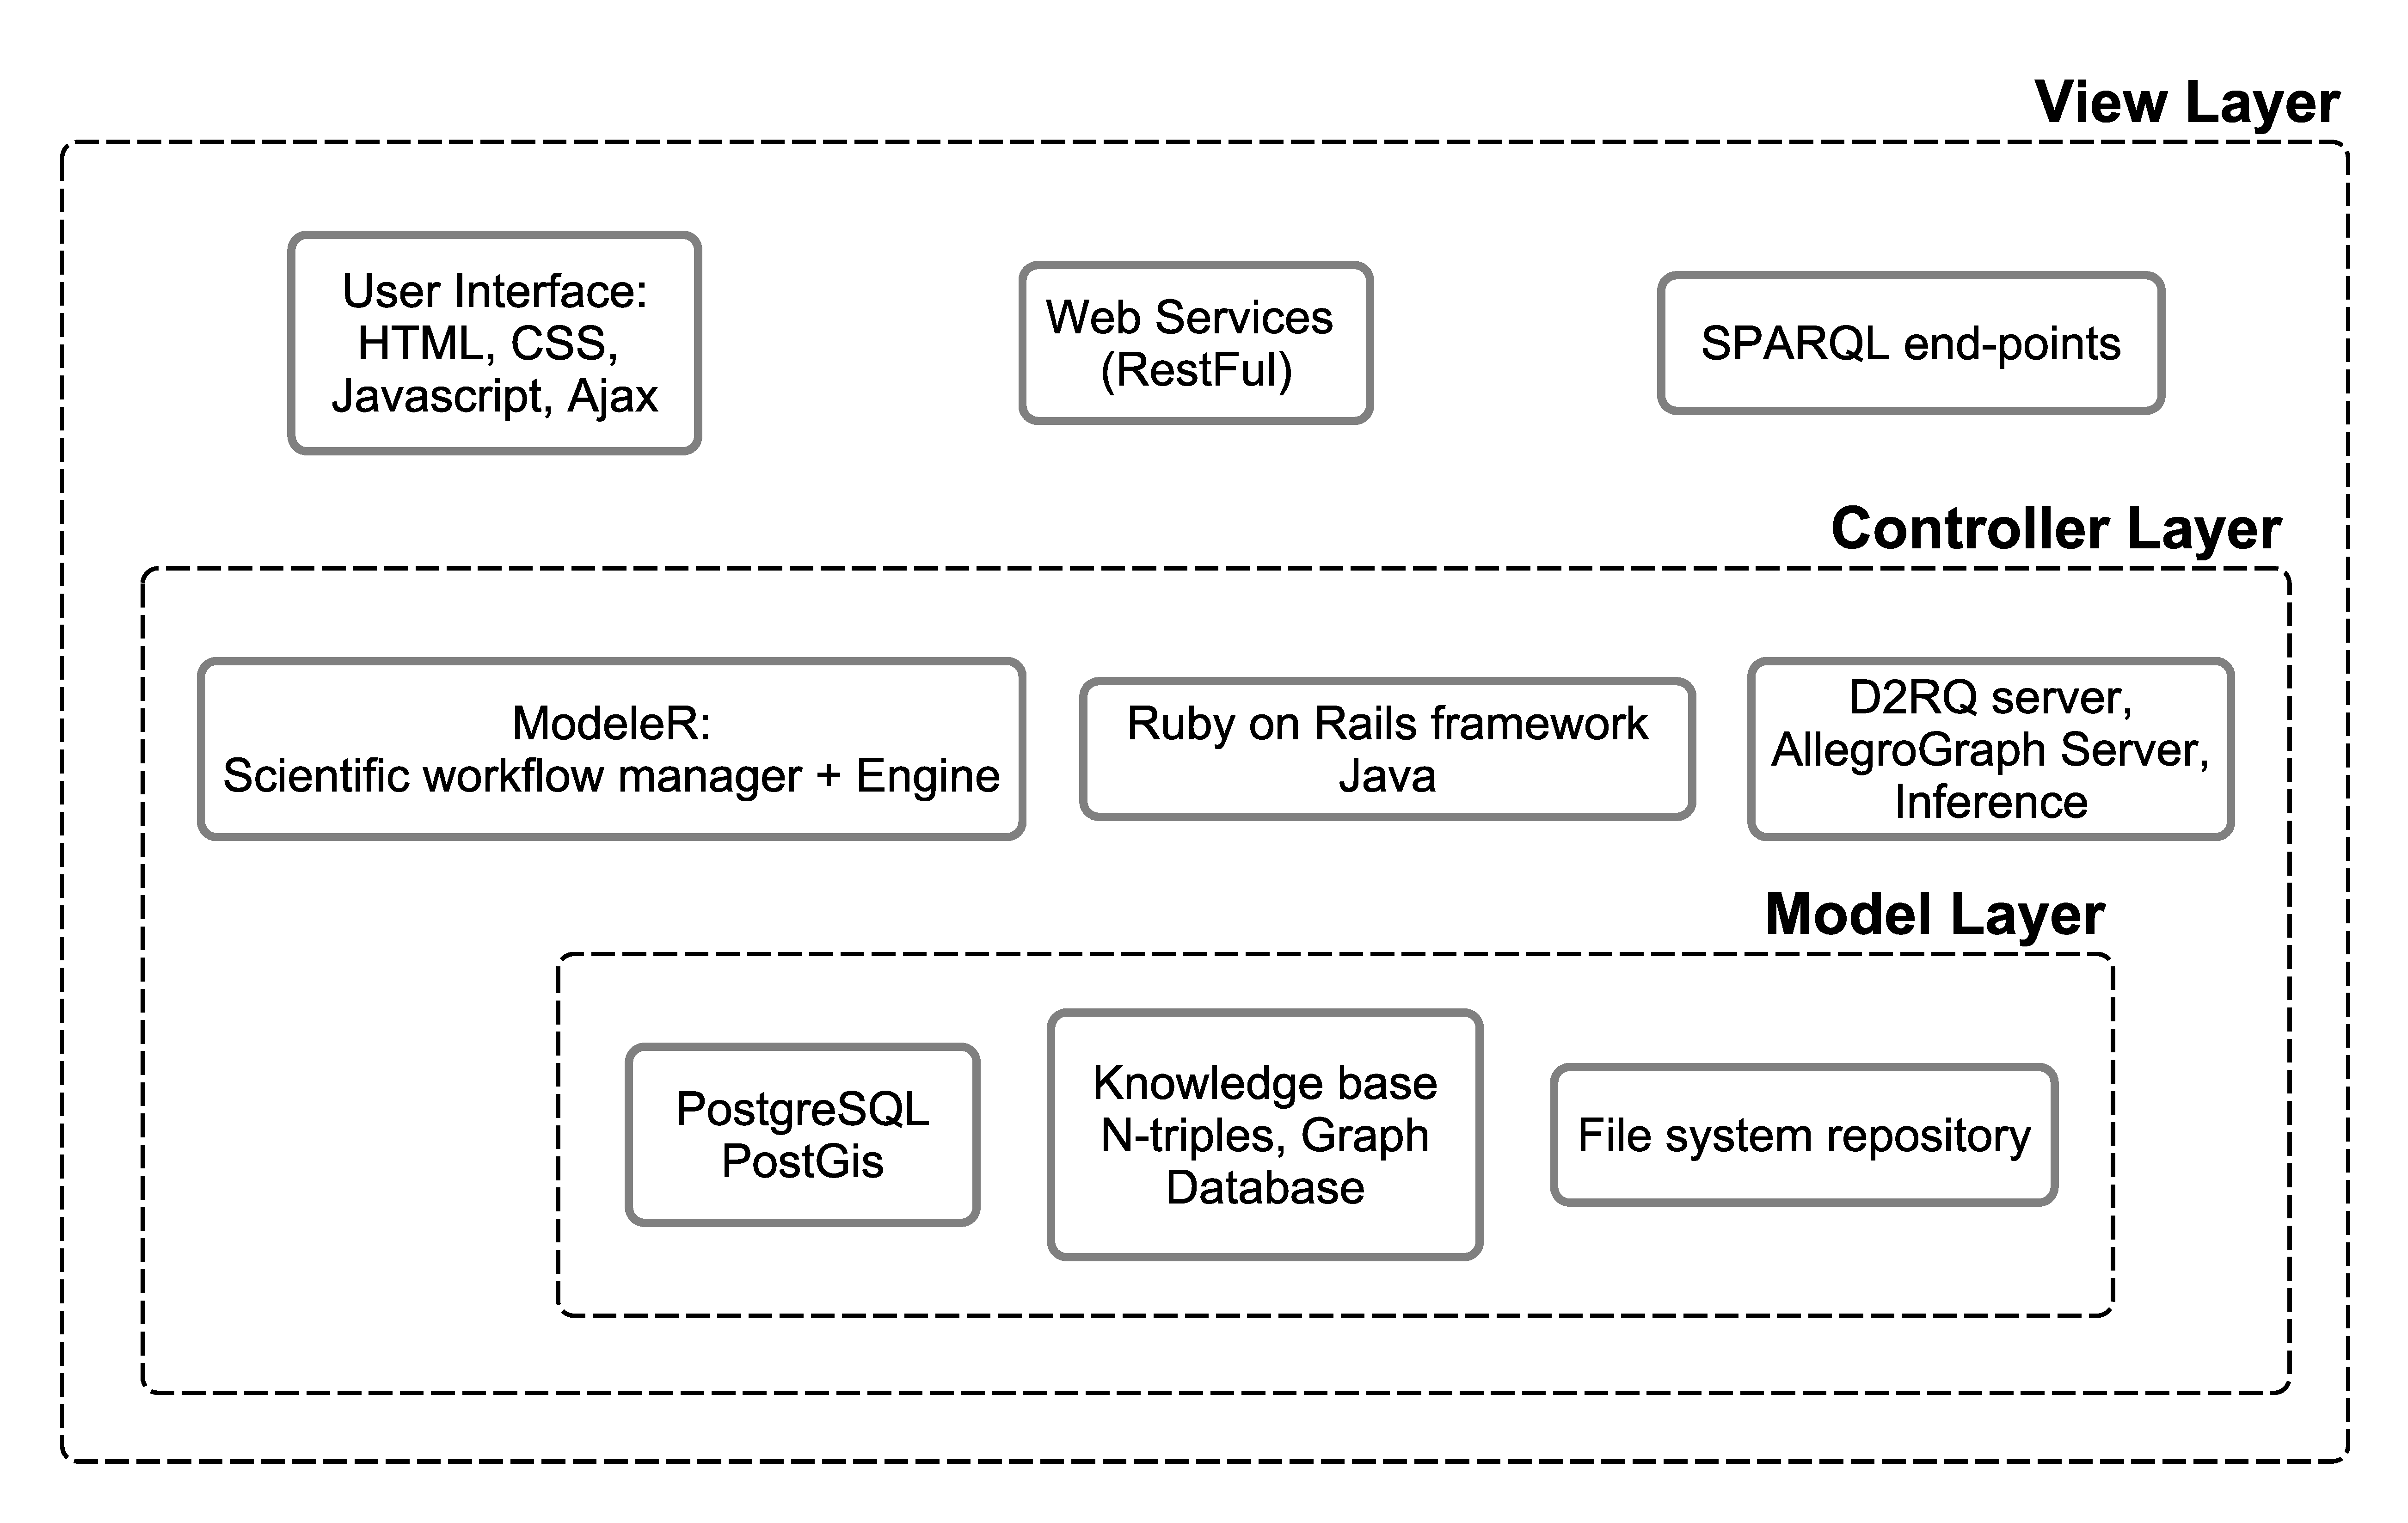
\includegraphics[width=\textwidth]{img/onto/onto-architecture}\caption{System architecture.}\label{fig:onto:architecture}
\end{figure}

subsection{Embedding MODIS images in a database and calculating thematic indicators}\label{sec:onto:Embedding}

HDF (Hierarchical Data Format) files are downloaded from NASA servers and processed using a workflow that makes the process automatic and reproducible. This workflow is stored and documented in a model repository called ModeleR \autocite{Bonetetal2014DocumentingStoring,PerezPerezetal2012ModeleREnviromental}. The workflow extracts information contained in any HDF files and stored it in a relational database (see structure in \figref{fig:onto:database}). NDVI and NDSI values are stored in a table that is linked to a vector layer containing the centroids of MODIS pixels. These raw data are used to aggregate and calculate the different indicators in Savia. The results are integrated again into the relational database, that is part of the Sierra Nevada LTER site information system \autocite{BonetGarciaetal2011SierraNevada}.\\
The indicators described in Section 2.2 were calculated for each pixel and temporal stage (by hydrological year, \emph{i.e.} the period between October 1st of one year and September 30th of the next; and by season) using SQL queries. The temporal trend for each pixel was calculated using the nonparametric Mann-Kendall trend test \autocite{Kendall1970RankCorrelation,Mann1945NonparametricTests}. The analyses were computed in R \autocite{RCoreTeam2013LanguageEnvironment} with Kendall package \autocite{McLeod2011KendallKendall}. We set 0.05 the alpha level for the test, and slopes with p-values \textgreater{} 0.05 were considered significant.

\begin{sidewaysfigure}
\centering
\includegraphics[]{img/onto/onto-database}\caption{Database schema. For each MODIS product the relational model stores three types of information: (i) spatial distribution of the pixels (\emph{nie\_malla\_modis} and \emph{iv\_malla\_modis} tables); (ii) values of NDVI and NDSI from original HDF files (\emph{nie\_mod10a2s} and \emph{iv\_modis} tables); and (iii) the metadata associated with each original image (\emph{nie\_metadatos\_modis} and \emph{iv\_metadatos} tables). The database also contains an auxiliary table to manage spatial entities (\emph{i.e.} \Qpy patches). Finally, there was a set of tables containing the aggregated information and indicators obtained after processing the raw data (see Section 2.2) (tables \emph{iv\_tendencias}, \emph{iv\_indices}, \emph{nie\_inicios}, \emph{nie\_fusions}, \emph{nie\_tendencias})}\label{fig:onto:database}
\end{sidewaysfigure}

\subsection{Creating the ontology}\label{sec:onto:Creating}

The ontology must represent both the information (MODIS products, indicators, and temporal trends) and the concepts used to add ecological meaning to the data (\figref{fig:onto:ontology}). To build the ontology, we used Time Ontology in OWL (Web Ontology Language) \autocite{HobbsPan2004OntologyTime} and Basic Geo (WGS84 lat/long) Vocabulary \autocite{Brickley2003BasicGeo} external ontologies. The OWL-Time ontology promoted by W3C (World Wide Web Consortium) \autocite{W3C2013LargeTriple}, provides a vocabulary for expressing instants and intervals, together with information concerning durations and date/time information \autocite{HobbsPan2004OntologyTime}. The Basic Geo is an RDF (Resource Description Framework) vocabulary for representing latitude, longitude, altitude information as well as other information related to spatial-located items.

Thus, the ontology takes into account three different parts (\figref{fig:onto:ontology}):

\begin{enumerate}
    \item Representing spatial information. The main concept is the Pixel, which represents a pixel from a MODIS image. Some pixels that share similar functions (\emph{i.e.} be covered by the same habitat) may belong to a Patch. Finally, some patches sharing the same dynamics may belong to a Group. The properties called \emph{PixelBelongsToPatch} and \emph{PatchBelongsToGroup} help to define the relationships between the previously defined concepts. \emph{PixelIsNearTo} is another useful property that adds the functionality of proximity to any pixel. The distance threshold used was 500 m between pixels (500 m is the spatial resolution of MODIS snow products). This property is symmetric because when a pixel A is near B, B is also near A.
    \item Indicators. This part contains a concept (\emph{IndicatorValues}) that represents the different values that take an indicator (see Section 2.2) at a given time point (through the concept called time: Year and the property \emph{HasYear}) and in a given place (through the concept Pixel and the property \emph{IndicatorValuesLocateInPixel}). We have also included a concept to describe all the indicators (Snow-cover duration, Snow-cover onset date, NDVI\_i annual, Maximum NDVI, etc.). These concepts are grouped according to their thematic area (Snow and Vegetation). Each indicator has a property called value that is measured using a given specific unit.
    \item The temporal trends are described in a concept called \emph{IndicatorTrend}. This concept shows the temporal trend of a single point for the whole time series (it is linked to \emph{Pixel} via \emph{PixelHasIndicatorTrends}). We have also created a concept for each temporal trend calculated for the previously described indicators (Trend of Snow cover duration, Trend NDVI\_i annual, etc.). These concepts are also grouped according to their thematic area (Snow Trend, Vegetation Trend). All these concepts have the following properties:
    \begin{enumerate}
        \item \emph{value\_tau} and \emph{p\_value}: These properties contain the statistic (\emph{value\_tau}) and the significance (\emph{p\_value}) reached by the Mann-Kendall trend analysis.
        \item \emph{value\_trend}: Categorical property ranges from -1 (significant negative trend) to 1 (significant positive trend). It is calculated according to the values of \emph{value\_tau} and \emph{p\_value.}
    \end{enumerate}
\end{enumerate}

This schema was implemented using OWL DL (Description logic) that allows an enhanced expression level and does not limit the values for cardinality \autocite{Smithetal2004OWLWeb}. The structure of the ontology created can be downloaded following this link: \url{http://iecolab.es/indicators.rdf}

\begin{sidewaysfigure}
\centering
    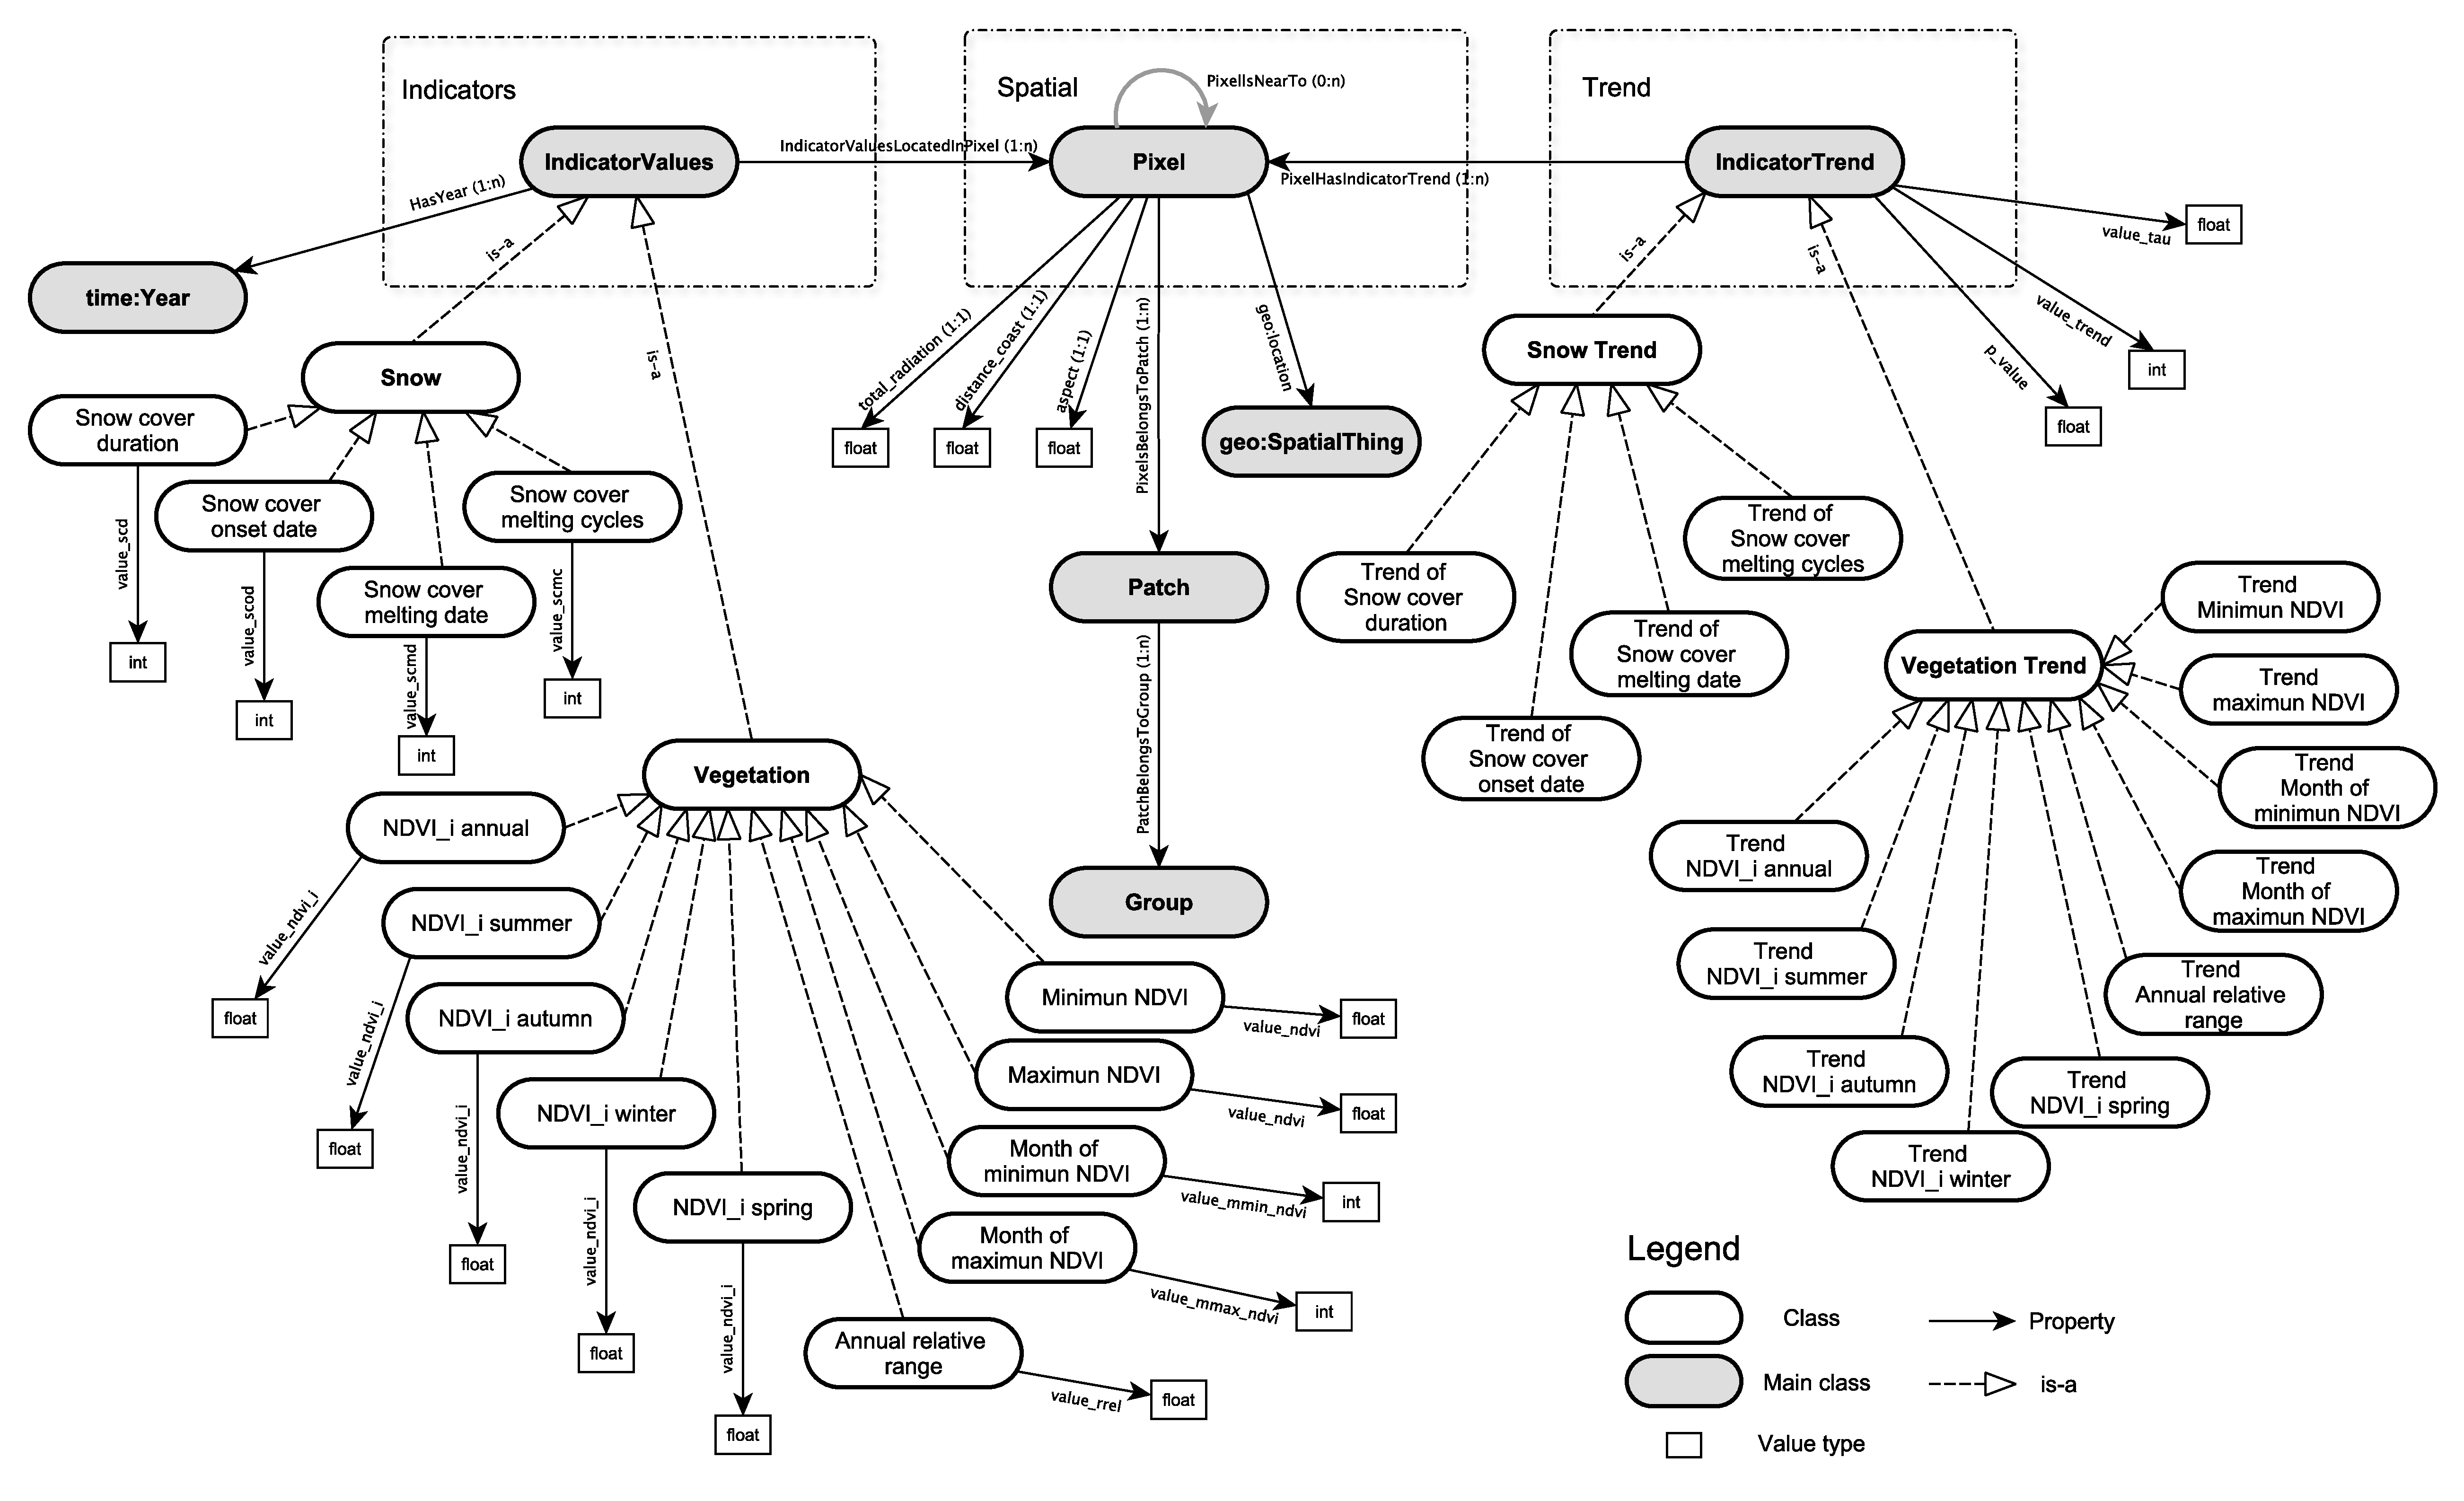
\includegraphics[width=\textwidth]{img/onto/onto-ontology}\caption{Detailed representation of the ontology created. Three main parts are considered:  spatial information, indicators, and temporal trends of the indicators}\label{fig:onto:ontology}
\end{sidewaysfigure}

\subsection{Knowledge base, SPARQL endpoint and inference}\label{sec:onto:SPARQL}

The next step after creating the ontology is to map the records in the database that contain the data to the ontology. Firstly, we used D2RQ \autocite{Bizeretal2004D2RQTreating} to map the relational database to OWL ontology. This software allows instance data to be retrieved from relational databases on-the-fly during the execution of SPARQL queries. Nevertheless, this procedure is time consuming and demands powerful computational capabilities. Thus, we dumped the mapping created with D2RQ into an intermediate N-triples file to avoid this drawback \autocite{Sarkaretal2011LinkedData}. This file was created with the data existing in the database and has all the triplets contained in the knowledge base.

To store the knowledge base, our tests with the open-source Apache Fuseki and Jena (\url{http://jena.apache.org/}) frameworks yielded unsuccessful results as soon as the data volume started to grow. Because we need an efficient implementation that can be scaled to large, enterprise-class data \autocite{Wilkinsonetal2004EfficientRDFa}, we also conducted some tests with AllegroGraph (\url{http://www.franz.com/agraph/allegrograph/}) and Virtuoso (\url{http://virtuoso.openlinksw.com/}), choosing the former option because of its capabilities and user-friendly management environment. This software is a triplestore that uses a graph database and it has the ability to encode values directly into its triples.
To enhance the results of the queries, a reasoning task can be also triggered within the generation of the system output process. AllegroGraph provides a built-in inference engine that derives implicit information from the knowledge base. Thus, users can easily turn it on by toggling that option in the query builder interface to enrich their queries. The inference engine is useful to find relations on different types of indicators and other implicit properties such as \emph{PixelIsNearTo}. For example, Savia can answer questions concerning implicit knowledge of pixels with a positive trend on seasonal mean of NDVI near others with a negative trend in snow-cover melting dates.

\section{Study Case}\label{sec:onto:CaseStudy}

For the improvement of the conservation status of habitats, it is necessary to implement management plans according to the Annex 6 of the Habitats Directive. Our system provides knowledge useful to design those management plans. We have used \Qp forests in Sierra Nevada (Spain) to explore the importance of snow duration in the functioning of \Qp forests. We have chosen this habitat as a case study for two reasons: \emph{a)} its interesting ecological dynamics (deciduous forest in a Mediterranean mountain), and \emph{b)} the need to manage these forests in a global-change context.

We have structured the case study according to three questions that will provide two types of results. Some of them will help in the understanding of the ecological functioning of the target habitat. And others will demonstrate how ontologies are useful tools to make remote sensing information more accessible for non-expert users.

\subsection{Which pixels show a trend towards higher productivity in summer?}\label{sec:onto:Trends}

\Qp forests show a well-defined growth season centred in summer \autocite{Alcarazetal2006IdentificationCurrent,Dionisioetal2012SatelliteBasedMonitoring}. Some works have pointed out changes in habitat functioning: increase in annual vegetation greenness in Sierra Nevada \autocite{AlcarazSeguraetal2008TrendsSurface,AlcarazSeguraetal2010EvaluatingConsistency} and seasonal functional changes in \Qp woodlands \autocite{Marty2008RegimeShift}, during the last decade.

This question aims to explore whether our target habitat is undergoing changes in summer productivity, specifically which \Qp forests of Sierra Nevada have shown a positive trend of the value of summer productivity (summer NDVI).

\begin{sidewaysfigure}
\centering
\includegraphics[width=.8\textwidth]{img/onto/onto-case-study}\caption{Scheme showing how the ontology solves questions regarding habitat functioning (a) and the behaviour of an abiotic factor (b). For each ecological question, different ontology elements are used to answer it. Then SPARQL language is used to query the knowledge base. Finally, results can be shown in different formats: map, csv or histogram. See first and second question of the study case. All pixels are displayed on the resulting map, but for those that have a significant positive trend the tau value is retrieved. In the map, we show seven different colours corresponding to this classification of tau values: [1, 0.5], [0.5, 0.25], [0.25, 0.05], [0.05, -0.051], [-0.051, -0.251], [-0.251, -0.501], [-0.501, -1].}\label{fig:onto:casestudy}
\end{sidewaysfigure}

\subsection{Which pixels show a trend towards an earlier snowmelt?}\label{sec:onto:Snowmelt}

Several studies have pointed out a trend towards higher temperatures and lower precipitation for the Mediterranean area \autocite{GarciaRuizetal2011MediterraneanWater,GiorgiLionello2008ClimateChange}. Significant declines in snow-cover extent and duration has been reported in some European mountains \autocite{Marty2008RegimeShift,MorenoRodriguezetal2005EvaluacionPreliminar,Nikolovaetal2013ChangesSnowfall,Scherreretal2004TrendsSwiss}. Climate projections forecast an increase of +4.8ºC at the end of the 21st century \autocite{Benitoetal2011SimulatingPotential} for Sierra Nevada and it expected that snowmelt will occur earlier in the year and will be more rapid \autocite{GarciaRuizetal2011MediterraneanWater}.

The second question that we raised it concerns the observed changes in snowpack in Sierra Nevada. We are interested specifically in which pixels show a trend towards earlier snowmelt during spring-summer. This question is crucial, given that \Qp forests need water in summer for growth.

\subsection{Which \Qp patches show a trend towards a more productive summer and earlier snowmelt?}\label{sec:ontoProductive}

This question explores the relationships and co-occurrence between biological production and snow-cover features.

Snow-related variables can explain the distribution of plant communities in the landscape \autocite{Jonesetal2001SnowEcology}. This causal relationship is more important at high elevation \autocite{BonetGarciaCayuela2009SeguimientoCubierta} in Sierra Nevada. But snow cover also explains part of the ecosystem functioning. \textcite{Trujilloetal2012ElevationdependentInfluence} that vegetation greenness increases with snow accumulation. This relationship varies with elevation, reaching a maximum between 2000-2600 m.

Some works have pointed out the influence of snow on greenness in Pyrenean oak forests \autocite{AlcarazSeguraetal2009BaselineCharacterization,Dionisioetal2012SatelliteBasedMonitoring}, but to date we have found no studies that analyse the coupling between snow cover and forest greening. Water availability is a key issue on the distribution of \Qp \autocite{delRioetal2007BioclimaticAnalysis,Gavilanetal2007ModellingCurrent}. This combination of plant growth and water scarcity makes summer a critical season for the functioning of this habitat.

The third question assesses the capacity of our ontology to show relationships similar to those described above. We have explored the co-occurrence of significant trends in biological production and snow-cover melting date in \Qp forests. In other words, we have analysed which \Qp forests show a trend towards higher productivity and earlier melting date in summer.

\section{Results}\label{sec:onto:Results}

We translated the above questions from natural language into ontology. For the first and second questions (Sections 4.1 and 4.2) we used two concepts (\emph{Pixel}, \emph{IndicatorTrend}) and some properties describing these concepts (\emph{value\_trend}, \emph{value\_tau}, \emph{PixelHasIndicatorTrends}, \emph{Trend NDVI\_i summer}, \emph{Trend of Snow cover melting date}) included in the ontology. Specifically:

\begin{itemize}
\item
  \emph{``select all Pixel where IndicatorTrend is positive for summer NDVI-I indicator''} for question 4.1 (\figref{fig:onto:casestudy}a)
\item
  \emph{``select all Pixel where IndicatorTrend is negative for snow-cover melting date''} for question 4.2 (\figref{fig:onto:casestudy}b)
\end{itemize}

We used SPARQL language to query the knowledge base.

Regarding the first question, we found that 75\% of pixels had a positive significant trend for summer NDVI (\figref{fig:onto:casestudy}a). For these, more than 80\% showed a strong or very strong positive trend. In general, \Qp patches located on the north face of Sierra Nevada showed a higher amount of significant pixels than the southern ones did (see map in \figref{fig:onto:casestudy}a).

The second question showed that almost 70\% of the pixels covered by \Qp forests had a strong or very strong negative and significant trend towards an earlier melting date (\figref{fig:onto:casestudy}b). Similar to NDVI, the northern patches showed a higher amount of significant pixels than the southern ones.

The third question is more difficult to translate to the ontology because it takes into account two datasets and more concepts than the previous questions. We have included a concept called Patch, being a subset of pixels that share some ecological features (they belong to the same \Qp population). This question also includes other concepts already mentioned (\emph{Pixel}, \emph{IndicatorTrend}) and properties describing those concepts (\emph{value\_trend}, \emph{value\_tau}, \emph{PixelHasIndicatorTrends}). We also calculated the percentage of pixels per Patch that showed trends towards more productive summers and earlier snowmelt. These elements were used to translate the original question to another one that was more suitable for the ontology: select all Pixels where the \emph{IndicatorTrend} is positive for the summer NDVI-I indicator (\emph{Trend NDVI\_i summer}) and negative for snow-cover melting date (\emph{Trend of Snow-cover melting date}). We used SPARQL language to query the knowledge base. The results can be displayed both in a map and table format (\figref{fig:onto:casestudyQ3}).

Savia provides two types of answers for this question: \emph{a)} A table (\figref{fig:onto:casestudyQ3}) shows the different \Qp patches ranked according to the percentage of pixels having the described trends in summer productivity and snow-cover melting date. \emph{b)} A binary map showing the pixels (grouped by \emph{Patch}) that satisfy both conditions (\figref{fig:onto:casestudyQ3}). All the patches that share the same behaviour are considered as Groups.

\section{Discussion and Conclusions}\label{sec:ontoDiscussion}

The system that we have created adds a semantic component to remote-sensing images using ontologies to describe this information. Savia is an operational system that is available for any user via the web (\url{http://obsnev.es/ontologia/index}).
Our system implements a query builder user interface that allows users to build questions using SPARQL. It also includes a set of predefined questions to show its capabilities. Furthermore, users can select different output file formats to display results (csv, text or map). All the analytical procedures needed to run this system have been documented using a model repository called ModeleR \autocite{Bonetetal2014DocumentingStoring,PerezPerezetal2012ModeleREnviromental}. The ontology created reuses and extends public ontologies like OWL-Time and Basic Geo (WGS84 lat/long) Vocabulary. The database containing MODIS images was translated into facts within a knowledge base. This requires a mapping between the database and the concepts contained in the ontology. The dynamical queries to knowledge base, using the mapping tool, were one of the most relevant bottlenecks that we have found during the implementation of the system, and we finally used enterprise-ready software to optimise queries to the knowledge base. We also used an inference engine to solve complex queries that require using advanced properties in the ontology (transitivity and symmetry, mainly).

We tested the ontological system in a case study focusing on \Qp habitat in Sierra Nevada. We identified significant trends in summer NDVI for 75\% of pixels covered by the target habitat. These pixels were located mainly in northern-faced patches (aspect was calculated using DEM). These results could be explained by a different pattern of summer productivity among the \Qp patches. We have also described similar trends in snow patterns: 70\% of pixels show a significant and negative trend towards an earlier melting date. Most of those pixels are also located in northerly facing patches. This result could have several hydrological and ecological implications: a) water from the melted snow is available for vegetation earlier each year, which could help deciduous trees to overcome the summer drought, b) the ground is free of snow during a longer period each year, which could provide extra area to treeline communities for altitudinal shifts.

The ontology has also helped to unveil the co-occurrence of significant trends both in snow cover (abiotic factor) and ecosystem functioning (NDVI). Thus, western patches display a high percentage of pixels showing this co-occurrence. The ecological implications of this co-occurrence can be explained by arguing that the earlier snowmelt provides water to \emph{Q. pyrenaica }trees when they are in the middle of their growing season. This earlier amount of water supply encourages trees to be more productive in summer. On the other hand, the southern patches also show this co-occurrence in the opposite way: The lack of significant trends in summer productivity for southern patches could be explained by the lack of pixels with trends towards earlier snowmelt in these areas. Although these results are still preliminary, we have established a link between the status of an abiotic factor and the functioning of ecosystems. Some forest activities can be scheduled according to the trends observed. It could be useful, for example, to reinforce the western patches by planting \Qp trees. These new trees could take advantage of the productive summers in order to create denser forests. These ecological results are similar to others found in different habitats (Trujillo et al.~2012).

The results (both ecological and methodological) demonstrate that the information in the MODIS time series is useful to assess the functioning of a terrestrial Natura 2000 habitat. We have described the temporal behaviour of \Qp forests in Sierra Nevada, distinguishing among patches located in areas with different environmental conditions. We have also showed temporal trends in several functioning indicators. The trends discovered would help managers to assess the conservation status of this habitat. They can also build management plans using the knowledge provided by our ontology (\emph{i.e.} to decide where to locate plantations taking into account the productivity trends). We have also described the behaviour of a key abiotic factor: snow cover; and we calculated trends for several snow-cover related indicators (snow duration, snow-cover melting date, etc.). Those could help managers to identify places where snow-cover trends could change in the coming years. Finally, we have detected relationships between trends in habitat productivity and snow-cover melting date for the target habitat. All this knowledge is offered to users (mainly managers and scientists) through a web portal, the use of which does not require expertise in remote sensing. Thus, we believe that this work is a worthwhile example of a web-based expert system created using an interdisciplinary approach.

\begin{figure}
\centering
\includegraphics[width=\textwidth]{img/onto/onto-case-studyQ3.jpg}\caption{Scheme showing the process of answering a complex query by the ontology. The question takes into account trends in habitat functioning as well as trends in snow-cover melting date. We first show the concepts used by the ontology to answer the query, then the SPARQL code and finally the results found. The left branch provides a map showing those pixels with trends towards more productive summers and earlier snowmelt date. The right branch offers a table ranking the Pyrenean oak patches according to the percentage of pixels that satisfies both conditions.}\label{fig:onto:casestudyQ3}
\end{figure}   
% !TEX root = ../my-thesis.tex
%
\selectlanguage{english}  
\chapter{\textcolor{ctcolormain}{Ecosystem services provided by \Qpw oak forests. A study case from Sierra Nevada mountain range (southern Spain)}}\label{sec:es}

\mbox{}
\vfill
{\color{ctcolormain}\textbf{Antonio J. Pérez-Luque}}; José V. Roces-Díaz; F.J. Bonet \& Regino Zamora (Submitted to \emph{Forest Systems}.)


\newpage

\paragraph{Abstract} \mbox{} \\
\Qpy (melojo) forests are relevant part of the Iberian landscape and have suffered intense anthropic pressures causing modifications in their structure and composition. Historically they were exploited in coppice for charcoal, firewood, or they were thinned and even burned to create grazing areas. Abandonment of traditional exploitation since the middle of the last century has led to a decrease in anthropic pressure on these ecosystems. Paradoxically, some of these oak woodlands present a state of advanced degradation (stagnation of growth; scarce regeneration; etc), with stands with high densities and high biomass accumulation, increasing the fire risk. Taking into account this situation, and considering the vulnerability of this species to global change, it is necessary to find alternatives to the traditional uses of coppice management, particularly for those stands located in their rear edge, such us the oak woodlands of Sierra Nevada (southern Spain), due to their relevance for the species conservation. In this work we present a comprehensive review of the main ecosystem services (ES) provided by melojo oak forests. Then, using the Sierra Nevada (SN) melojo oak populations as study-case, we explore more in depth the ES provided by these woodlands. We combined expert knowledge and datasets from different sources (\emph{e.g.} grey literature, monitoring programs) to quantify the ES provided by these forests. We also explored the spatio-temporal pattern of some ES among the melojo oak populations within SN mountain range. Provisioning (\emph{e.g.} use of melojo oak wood in the wine production) and regulating services (\emph{e.g.} carbon sequestration and soil fertility) were widely reported in the literature review meanwhile no studies assessing cultural ES were found in our literature review. However, this pattern changes when the ES were analyzed in more detail as in our study case, highlighting the existence of diverse cultural services provided these forests in SN. We found differences among the supply of ES within the melojo oak populations, with southern populations have higher values of regulating services and northern ones exhibited higher values for cultural services. A temporal variation in the supply of ES of melojo forests was observed. Until the middle of the last century, provisioning services predominated over regulating and cultural services (poor valued). The abandonment of traditional activities led to a decrease of provisioning services in favor of regulating services, and in the last decades, cultural services. Our compilation of local scale data has allowed us to quantify many of ES supplied by the \Qp forests, which could aid to natural resource managers with more information and tools to help them in the decision-making process.
\newpage

\section{Introduction}\label{sec:es:intro}

Mediterranean forests are subjected to significant and simultaneous climatic and anthropogenic pressures \autocite{FAOPlanBleu2018StateMediterranean,DoblasMirandaetal2017ReviewCombination}, and climate change is expected to strongly affect the Mediterranean Region \autocite{GiorgiLionello2008ClimateChange,Crameretal2018ClimateChange,Crameretal2020ClimateEnvironmental}. Besides, the impacts of global change on Mediterranean forest ecosystems are altering the provision of ecosystem services \autocite{Lindneretal2010ClimateChange,Lindneretal2014ClimateChange,NoceSantini2018MediterraneanForest,Penuelasetal2017ImpactsGlobal,SerradaHierroetal2011ImpactosVulnerabilidad} particularly in mountainous regions, which have shown a high vulnerability to climate change \autocite{Schroteretal2005EcosystemService}. Notwithstanding, Mediterranean forests provide a wide range of ecosystem services (ES), and represent a great asset and opportunities for the future of the Mediterranean basin \autocite{Gauquelinetal2018MediterraneanForests,NoceSantini2018MediterraneanForest}. Hence, the importance of Mediterranean forests derives both from their current value in terms of area and goods and services, and from the potential role they are likely to play in the future as providers of ES \autocites{FAOPlanBleu2018StateMediterranean}.

Among the Mediterranean type forests, the oak woodlands, \emph{i.e.}, those dominated by oak tree species (\emph{e.g.} \emph{Quercus ilex}, \emph{Q. suber}, \emph{Q. robur}, \emph{Q. faginea}, \emph{Q. petraea}, \emph{Q. pubescens}, \emph{Q. pyrenaica}, \emph{Q. canariensis}) are key ecosystems providing variety of ES \autocite{Maranonetal2020IberianOaks}. For example, their capacity to sequester carbon and therefore to regulate the climate and to mitigate the effects of climatic change is a remarkable regulating service. Oak forests contribute to soil fertility and to the regulation of air, soil and water quality \autocite{Maranonetal2012EstadoTendencia}. These woodlands also provide several raw materials: cork, firewood, acorns \autocite{Bugalhoetal2011MediterraneanCork}. In addition, their role as providers of a wide variety of cultural services, such as recreational, aesthetic and spiritual has been also highlighted \autocite{Lofetal2016ManagementOak}. To conserve these forests and their biodiversity, and to manage them in a sustainable way, it is important to be aware of their real and potential supply of ES.

\subsubsection{The case of melojo woodlands (\Qpy) in the Western Mediterranean Region}\label{sec:es:intro-qp}
\Qpw (Pyrenean oak, \emph{melojo}) is a marcescent tree species widely distributed throughout southwestern France and the Iberian Peninsula with some populations at the mountain areas of northern Morocco \autocites{Franco1990Quercus} (\figref{fig:es:location}). In the Iberian Peninsula, these forests (in this chapter we will refer to \Qpy forests as \emph{melojo} oaklands or \emph{melojo} woodlands) occupy siliceous soils under meso-supramediterranean and mesotemperate areas and subhumid, humid, and hyperhumid ombroclimate \autocites{delaSernaetal2016MarcescentQuercus,Gavilanetal2018SclerophyllousDeciduous}. The rear-edge populations of this species are restricted to high-mountain areas where they persist as isolated nuclei with ecological conditions very different from those of the main distribution area \autocites{PerezLuqueetal2021EcologicalDiversity}. Sierra Nevada mountains (37°N, 3°W, Spain) represent one of the southernmost European limits for this species (Figure \ref{fig:es:location}b). In this mountain area, considered a glacial refuge for deciduous \emph{Quercus} species \autocite{Olaldeetal2002WhiteOaks}, there are eight melojo oak patches, occupying a total of 2400 ha, and ranging from 1100 to 2000 \emph{m.a.s.l.}. Among the forest ecosystems in Sierra Nevada, melojo woodlands are the richest regarding vascular plant species, containing a large number of endemic and endangered plant species \autocite{Loriteetal2008PhytosociologicalReview}. They also harbor high levels of intraspecific genetic diversity \autocite{ValbuenaCarabanaGil2013GeneticResilience,ValbuenaCarabanaGil2017CentenaryCoppicing}. 

\Qp woodlands, like other forests in Mediterranean area, have been subjected to intense anthropogenic pressures over time \autocite{GarciaJimenez20099230Robledales}, resulting in a reduction of their extension and a modification of their floristic composition \autocites{Serradaetal1992CoppiceSystem,Gavilanetal2000EffectsDisturbance,PerezLuqueetal2021EcologicalDiversity} and of their structural patterns \autocites{Calvoetal1999PostfireSuccession,Tarregaetal2006ForestStructure}. Historically, these woodlands have been exploited in coppices for obtaining several products such as firewood, charcoal, tannins, casca (\emph{i.e.} parts of the bark used to extract tannins), and many other traditional uses \autocites{RuizdelaTorre2006FloraMayor,SanchezPalomaresetal2008EstacionesEcologicas}. For instance, after the Spanish Civil war (since 1940's), some oak woodlands were massively cut down to use the firewood as fuel for automobiles (\emph{e.g.} Dehesa de San Jerónimo, Sierra Nevada)\autocite{Prieto1975BosquesSierra}. Forest management for coppices consisted of clear-cutting in rotation periods of 12-20 years, causing the profusion of shoots from the stool highly appreciated by livestock \autocite{Bravoetal2008SelviculturaMontes}. Thinning  and sometimes even burned have also been carried out to create pastures with low densities of mature trees that provide acorns, firewood and large areas for grazing \autocites{HerreraCalvo2016UsoPastoral,Alvarezetal2009CambiosEstructura,ValbuenaCarabanaGil2017CentenaryCoppicing}. In fact, overgrazing in these formations have caused strong soil erosion loss, which was noticed by forest managers since the end of the 19\textsuperscript{th} century \autocites{Laguna1872ComisionFlora}. In some areas, the strong anthropic pressure provoked the loss of the forest cover. For instance, in southern slopes of Sierra Nevada mountains, oak woodlands were almost completely removed at the beginning of the 20\textsuperscript{th} century, which led to some of its watershed being considered among the most torrential in Spain \autocites{RomeroZurbano1909DivisionHidrologicoforestal}. All these anthropogenic processes have transformed the melojo woodlands in a deep way that it is difficult to find stands that can be considered natural forests \autocites{RuizdelaTorre2006FloraMayor}. 

The abandonment of livestock and forestry traditional uses since the middle of the last century due to rural abandonment \autocites{MacDonaldetal2000AgriculturalAbandonment}, has caused a decrease in anthropogenic pressure on Mediterranean forests, being particularly important for mountain areas \autocites{JimenezOlivenciaetal2015MedioSiglo,JimenezOlivenciaetal2015EvolucionUsos,Piasetal2014ColonizationAbandoned,ValbuenaCarabanaetal2010HistoricalRecent}. Paradoxically, and considering this decrease in anthropogenic pressure, many of the oak stands present a state of advanced degradation, showing growth stagnation, lack of fruiting, and also signs of branch dieback \autocites{Canellasetal2004GrowthResponse, Bravoetal2008SelviculturaMontes, ValbuenaCarabanaGil2014EfectosGestion, PiqueVericat2015EvolutionPerspectives, Piqueetal2018Spain}. Many stands, derived from the high resprout capacity of \Qp, also have high tree density that would increase their vulnerability to drought, as has been reported in other forests across the world \autocite{McDowelletal2020PervasiveShifts}. The high tree density together with the accumulation of biomass and high horizontal continuity, would increase the risk of fire \autocites{Bravoetal2008SelviculturaMontes,GarciaJimenez20099230Robledales}. In addition, these problems may be aggravated in the current context of climate change (increase in temperatures and higher incidence of extreme events such as droughts) \autocites{IPCC2013ClimateChange,Spinonietal2018WillDrought}, particularly considering the high vulnerability of this species to climate change \autocites{Benitoetal2011SimulatingPotential,GarciaValdesetal2013ChasingMoving,SanchezdeDiosetal2009PresentFuture,GeaIzquierdoetal2013GrowthProjections}, and especially for areas located in the rear edge of their distribution range such as Sierra Nevada mountain range.

In view of this current situation of vulnerable (to global change drivers) forest stands, affected by the progressive abandonment of traditional land uses during the last decades, the need of defining alternative uses for melojo oak woodlands has been pointed out \autocites{MesonMontoya1985VegetacionForestal,SanMigueletal2012BosquesMatorrales}, and some management alternatives have been proposed \autocite[\emph{e.g.} sylvopastoral uses, see][]{HerreraCalvo2016UsoPastoral}. Melojo woodlands are human-shaped ecosystems with high conservation value, and consequently, management is required to guide their development \autocite{Hobbsetal2006NovelEcosystems}. In this sense, the identification and characterization of the main ES and their spatio-temporal pattern, becomes a crucial to develop landscape planning and forest management strategies in a global change context \autocites{Piqueetal2018Spain}. 

Ecosystem services provided by melojo woodlands depend on the intensity of human use. Both overuse and abandonment of melojo woodlands provided very different scenarios for the provision of ES and for the socioeconomic demand for them. Despite the wide variety of ES provided by oaklands is worldwide acknowledged, very little has been written specifically about the provision of ES by oak-dominated forests \autocites{Maranonetal2012OakTrees,Maranonetal2012EstadoTendencia,MorenoLlorcaetal2012MontanaMediterranea}. Some works have carried out a general valuation of the ES provided by the different \emph{Quercus} woodlands at regional and national scales \autocite{SanMigueletal2012BosquesMatorrales,Maranonetal2012EstadoTendencia,Sousaetal2020EcosystemServices}, and some studies provided temporal trend analysis of ES from an economic perspective \autocites[see][for an example for woodland pastures of California and Spain]{Caparrosetal2013EconomicsEcosystem}. However, to our knowledge, there is no comprehensive review of the ES provided by \Qp woodlands. 

The aim of this work is to carry out a review of the main ES provided by \Qp woodlands. Firstly, we conducted a literature review to know the general state of the art and to summarize some of the most relevant ES provided by these formations. Secondly, using the Sierra Nevada oak populations as study-case we explore more in depth the ES provided by these woodlands. For this purpose, we combined expert knowledge and a wide variety of data coming from ecological monitoring programs and several research projects to quantify as far as possible the ES provided by these forests. We are also interested in exploring how the ES are spatially distributed in this mountain region. For this, we searched for differences on the supply of ES between the melojo oak populations within Sierra Nevada mountain range.  Finally, using time series of several indicators, we have assessed the temporal changes of ES supply by \Qp in our study area.  

\begin{figure}
    \centering
    \includegraphics[width=\textwidth]{img/es/es-mapa_spain_sn.jpg}
    \caption{\textbf{(a)} Distribution of \Qpy forests in the Iberian Peninsula, and location of the oak populations in Sierra Nevada mountain range \textbf{(b)}. In Sierra Nevada three oak populations clusters have been identified \autocite{PerezLuqueetal2021EcologicalDiversity}: N=Northern (CAM: Camarate); NW = Northwestern (GEN: Genil, MON: Monachil, DIL: Dílar, DUR: Dúrcal); S=Southern (CAÑ: Cáñar, POQ: Poqueira; TRE: Trevélez). Source: Spanish National Forest Map (1:50.000).}\label{fig:es:location}
\end{figure}

\section{Material and methods}\label{sec:es:mat}
\subsubsection{Study area}\label{sec:es:mat-studyarea}
Sierra Nevada is a mountainous region located in the south-eastern Iberian Peninsula  (37º14'-36º54'N; 2º37'-3º39'W) covering more than 2000 km\textsuperscript{2} with an elevation range of between 860 and 3482 \emph{m.a.s.l.}. The climate is Mediterranean, characterized by cold winters and hot summers, with a pronounced summer drought. The annual average temperature decreases in altitude from 12-16 ºC below 1500 \emph{m.a.s.l.} to 0 ºC above 3000 \emph{m.a.s.l.}. Annual precipitation ranges from less than 250 mm in the lowest areas of the mountain range to more than 700 mm in the highest peaks. Winter precipitation is mainly in the form of snow above 2000 \emph{m.a.s.l.}. Topographically, the area is heterogeneous, with strong climatic contrasts between the sunny, dry south-facing slopes and the shaded, wetter north-facing slopes. This mountain range is considered one of the most important biodiversity hotspots in the Mediterranean region \autocite{Blancaetal1998ThreatenedVascular}, hosting 105 endemic plant species for a total of 2353 taxa of vascular plants (33\% and 20\% of Spanish and European flora, respectively) \autocite{Lorite2016UpdatedChecklist}. Forest cover in Sierra Nevada is dominated by pine plantations (\emph{Pinus halepensis} Mill., \emph{Pinus pinaster} Ait., \emph{Pinus nigra} Arnold subsp. \emph{salzmannii} (Dunal) Franco, and \emph{Pinus sylvestris} L.) covering approximately 37000 ha. Native forests are mainly dominated by holm oak (\emph{Quercus ilex} subsp. \emph{ballota} (Desf.) Samp.) occupying low and medium mountain areas, and melojo oak ranging from 1100 to 2000 \emph{m.a.s.l.} \autocite{PerezLuqueetal2019MapEcosystems}.

\begin{table}[]
\centering
\caption{Indicators used to evaluate the temporal evolution of the ES supply by \Qp woodlands in Sierra Nevada. All data referred to Robledal de Cáñar oak woodland (southern slope of Sierra Nevada), except visitors numbers corresponding to all Sierra Nevada Protected Area. For each indicator the ES category are indicated: (R) regulation; (S) provisioning and supporting; (C) cultural.}
\label{tab:es:temporal}
\footnotesize
\begin{tabular}{>{\raggedright\arraybackslash}p{0.2\textwidth}>{\raggedright\arraybackslash}p{0.2\textwidth}>{\raggedright\arraybackslash}p{0.4\textwidth}>{\raggedright\arraybackslash}p{0.2\textwidth}}
\toprule 
\textbf{Indicator} & \textbf{Units} & \textbf{Data Source - References} & \textbf{Temporal range} \\
\toprule
Population & Inhabitants & Institute of Statistics and Cartography of Andalusia & 1940 - 2016 \\
Apiarian uses (S) & Number of hives & Public Forest use plans. \citet{MorenoLlorcaetal2014CaracterizacionFuentes,MorenoLlorcaetal2016HistoricalAnalysis} & 1978 - 2011 \\
Acorn harvesting (S) & Hectoliters & Public Forest use plans. \citet{MorenoLlorcaetal2014CaracterizacionFuentes,MorenoLlorcaetal2016HistoricalAnalysis}; \citet{MesaTorres2009} & 1950 - 1966 \\
Sheep farming (S) & Number of animals & \citet{MorenoLlorcaetal2014CaracterizacionFuentes,MorenoLlorcaetal2016HistoricalAnalysis}; \citet{MesaTorres2009} & 1950 - 2011 \\
Visitors numbers (C) & Visitor numbers & Sierra Nevada Natural and National Protected Area & 1999 - 2019 \\
EVI vegetation Index (R) & dimensionless & MODIS; \citet{PerezLuqueetal2015OntologicalSystem,PerezLuqueetal2020LanduseLegacies} & 2000 - 2016 \\
Biomass increment(S) & Mg ha$^{-1}$ year$^{-1}$ & Spanish NFI. \citet{PerezLuqueetal2021ManualGestion} & 1995 - 2007 \\
Forest Area (S, R) & ha & \citet{NavarroGonzalezetal2012CartografiaHistorica} & 1956 - 2007 \\
Oak tree density (S) & n trees ha$^{-1}$ & \citet{Zamoraetal2017MonitoringGlobal} & 1956 – 2005
\end{tabular}
\end{table}


\subsubsection{Selection of ecosystem services and their assessment }\label{sec:es:mat-selection}
To analyze the ES provided by melojo forests, we have carried out two different phases. Firstly, we performed a general literature review to explore the state of the art on the ES provided by these forests regardless of their specific location. Secondly, considering the results of the general literature review, we have carried out a more comprehensive analysis of the ES provided by the melojo forests in Sierra Nevada. We have characterized their supply for Sierra Nevada mountain region, and where data were available, we have quantified them, and compared between melojo populations identified in Sierra Nevada. Finally, we explored temporal evolution of indicators for several ES when data were available. For the classification and definition of ecosystem services, we used the CICES V5.1 (Common International Classification of Ecosystem Services) approach \autocites{HainesYoungPotschin2018CommonInternational}. We have considered three categories of ecosystem services: provisioning, regulating and cultural, and for each of them, we have identified different ES indicators. Due to the large number of ES studied, we have considered it more practical to explain for each of the ES, the indicator(s) used to quantify it (see details in the following section).  

To characterize the scientific literature that evaluate the ES of the melojo oak woodlands, we performed initially a systematic search in the ISI Web of Knowledge (search date: October 2020). We compiled references published in indexed journals included in the Journal of Citation Reports (JCR), in English language, since 1970 to 2020, that evaluated a wide variety of ES indicators in these woodlands. First, we conducted a search for papers on the study species with the term \emph{"Quercus pyrenaica"} in the title, keywords or abstract, which produced 393 results. We applied a second criterion, to extract papers that analyzed possible services, including a broad list of terms (also in the title, keywords or abstract) related to ES
(\tabref{tab:es:wos}). The combination of both produced 188 results. After reviewing their abstracts, we selected 60 papers that met the premise of evaluating ES in melojo oak woodlands (\tabref{tab:es-review}). We omitted papers focused exclusively on descriptive aspects of these ecosystems (\emph{e.g.} floristic composition or ecosystem structure), their biodiversity (\emph{e.g.} species richness) which were not directly related to ecosystem service indicators. 

For each of the ES reviewed, we initially described the general status of the services in these woodlands using the compiled references. Then, we performed a quantification for the Sierra Nevada oak woodland populations, when data were available. The values for the quantification were obtained both from the literature review and from several research datasets in combination with the expert criterion (\tabref{tab:es:data}). For those ES with data availability, we performed a quantification using a spatiotemporal approach: \emph{i)} we assessed how ES provision varies across the space in each of the oak population clusters identified in Sierra Nevada (\emph{i.e.} Northern (N), Northwestern (NW), and Southern (S)) \autocite[ see][]{PerezLuqueetal2021EcologicalDiversity}; and \emph{ii)} we explored the temporal variation in the provision of ES using available time series of several indicators of ES (\tabref{tab:es:temporal}). 


\begin{sidewaystable} 
\caption{Ecosystem Services (ES) indicators used in this study. For each indicator the ES category, references, units, and data source are indicated. (\emph{R}): regulation; (\emph{S}): provisioning and supporting; (\emph{C}): cultural. (*) extracted from the literature; (**) own calculations. (+) indicators with data for oak populations of Sierra Nevada.}\label{tab:es:data}
\centering
\scriptsize
\begin{adjustbox}{width=\linewidth}
\begin{threeparttable}
\begin{tabular}{>{\raggedleft}m{0.087\linewidth}>{\centering}m{0.108\linewidth}m{0.4\linewidth}>{\centering}m{0.102\linewidth}m{0.165\linewidth}m{0.071\linewidth}}
\textbf{Ecosystem Service} & \textbf{ES indicator used} & \textbf{Bibliographic References} & \textbf{Units} & \textbf{Data Source} & \textbf{Data for Sierra Nevada } \\ \toprule 
Experiential use of Landscape (C) & Number of photographies (*) & \autocite{MorenoLlorcaetal2020EvaluatingTourist} & Number of photographies & \autocite{RosCandeiraetal2020SocialMedia} & Yes (+) \\
Physical use of Landscape (C) & Wikiloc tracks (**) &  & Routes density; Total routes & Wikiloc & Yes (+) \\
Recreational (C) & Visitors numbers (**) &  & Visitor numbers & Sierra Nevada Natural and National Protected Area & Yes (+) \\
Scientific (C) & Research requests permisision (**) & \autocite{Zamoraetal2016GlobalChange} & Number of Research requests & Sierra Nevada Natural and National Protected Area & Yes (+) \\
Scientific (C) & Density of socio-ecological monitoring methodologies (**) & \autocite{Zamoraetal2016GlobalChange} & Density of monitoring methdologies & Sierra Nevada Natural and National Protected Area & Yes (+) \\
Symbolic (C) & Singular trees (*) & \autocites{IruritaFernandezetal2003ArbolesArboledas, SanchezGarciaetal2003ArbolesArboledas} &  & Andalusia Regional Goverment & Yes \\
Biodiversity (S) & Bird richness (**) & \autocites{BareaAzconetal2012PasseriformesOtras,PerezLuqueetal2016DatasetPasserine,ZamoraBareaAzcon2015LongTermChanges,PerezLuqueetal2021ManualGestion} & Species number & Sierra Nevada Global Change Observatory & Yes (+) \\
Biodiversity (S) & Fungal diversity (*) & \autocites{Ortegaetal2010MycorrhizalMacrofungi, MorenoArroyo2004InventarioMicologico} & Species number & Basic Mycological Inventory of Andalusia &  \\
Biodiversity (S) & Genetic diversity (*) & \autocites{ValbuenaCarabanaGil2013GeneticResilience,ValbuenaCarabanaGil2013ReduceAprovechamiento,ValbuenaCarabanaGil2014EfectosGestion,ValbuenaCarabanaGil2017CentenaryCoppicing} &  &  & Yes (+) \\
Biodiversity (S) & Microbial diversity (*) & \autocites{CoboDiazetal2017TaxonomicFunctional,Lasaetal2019BacteriaEndosphere, Lasaetal2019MetabarcodingReveals} &  &  & Yes \\
Biodiversity (S) & Woody richness (*) & \autocite{PerezLuqueetal2014SinfonevadaDataset,Loriteetal2008PhytosociologicalReview} & Species number &  & Yes (+) \\
Food provision (S) & Wild mushrooms production (*) & \citet{RayaLopezetal2017MuestreosPara} & kg Fungi ha$^{-1}$ year$^{-1}$ & Plan CUSSTA (Plan for the Sustainable Use and Conservation of Mushrooms and Truffles in Andalusia) & Yes \\
Tanning (S) & Percentage of tannins (*) & \autocites{FernandezdeSimonetal2006ChemicalCharacterization,Doceetal2007EffectImmature,TornerOchoa1952CurtientesVegetales} & \% of tannis present at bark &  & \\ 
Timber (S) & Biomass increment & \autocite{PerezLuqueetal2021CarbonSequestration} & Mg ha$^{-1}$ year$^{-1}$ & Spanish National Forest Inventory & Yes \\
Wine Ageing (S) & Phenological compunds (*) & \autocites{Ramiloetal2017VolatileOrganic,Gallegoetal2012PhenolicCompounds, CadahiaFernandezdeSimon2004UtilizacionRoble,FernandezdeSimonetal2008VolatileCompounds,FernandezdeSimonetal2009VolatileCompounds, Gallego2013EstudioPotencial,MartinezGiletal2020EffectSize} &  &  &  \\
Climate Regulation (R) & Carbon sink (**) & \citet{PerezLuqueetal2021CarbonSequestration} & Mg CO$_2$ ha$^{-1}$ & LIDAR and Forest Inventories & Yes (+) \\
Climate Regulation (R) & Vegetation Index (NDVI, EVI) (*) & \autocites{Dionisioetal2012SatelliteBasedMonitoring,AlcarazSeguraetal2016ChangesVegetation,PerezLuqueetal2015OntologicalSystem,Cazorlaetal2020RemoteSensingbased} &  & MODIS & Yes (+) \\
Climate Regulation (R) & Regulation of temperature (**) & \autocite{Zamoraetal2021UniendoMacro} &  & ClimaNevada & Yes \\
Control of erosion (R) & Soil erosion Control (*) & \autocites{MesonMontoya1985VegetacionForestal,Salomonetal2017GeneralFailure} &  &  &  \\
Soil Fertility Regulation (R) & Soil Organic Carbon (**) & \citet{Hengletal2017SoilGrids250mGlobal, Batjesetal2017WoSISProviding, Batjesetal2020StandardisedSoil} & Mg SOC ha$^{-1}$ & SoilGrid database & Yes (+) \\
\bottomrule
\end{tabular}
\end{threeparttable}
\end{adjustbox}
\end{sidewaystable}

\section{Ecosystem Services provided by \Qp woodlands}\label{sec:es:results}
The compilation of literature carried out has shown us those services that have been most frequently evaluated in works focused on \Qp woodlands (see \tabref{tab:es:wos}). Provisioning services were the most frequently ES evaluated within the 60 papers selected in the literature review. Among them, the studies focused on investigating the effect of melojo wood in the wine production process stand out (\emph{n} = 26/60) \autocites[\emph{e.g.}][]{FernandezdeSimonetal2010CharacterizationVolatile,CastroVazquezetal2013EvaluationPortuguese}, since barrels are frequently built with the wood of this species. In addition, we found different studies evaluating mushroom production \autocites[\emph{e.g.}][]{OriadeRuedaetal2010CouldArtificial}, the effect of this species on livestock production \autocites[\emph{e.g.}][]{Nunezetal2012LivestockManagement}, or the production of wood or biomass for energy (\emph{n} = 6/60) \autocites[\emph{e.g.}][]{Mirandaetal2009EnergeticCharacterization}. Regarding regulation services, several studies assessed the role of forests in soil quality and fertility (\emph{n} = 12/60), or their capacity for carbon sequestration and storage \autocites[\emph{n} = 12/60; \emph{e.g.}][]{Alvarezetal2014InfluenceTree}. There also a high proportion of studies on soil carbon \autocites[\emph{n} = 8/60; \emph{e.g.}][]{Fonsecaetal2019ImpactTree}. Finally, it should be noted that, applying the above-mentioned search criteria, no studies on the evaluation of cultural services in the melojo woodlands have been found.

\begin{figure}
    \centering
    \includegraphics[width=\textwidth]{img/es/es-fig_2_mapas.jpg}
    \caption{\textbf{(a)} Distribution of the Soil organic carbon in Sierra Nevada. Oak populations in white. Drawn with data from SoilGrid database \autocites[see][]{Hengletal2017SoilGrids250mGlobal}. \textbf{(b)} Density of Wikiloc routes for the municipalities of Sierra Nevada (Data from January 2020). Data are shown in Logarithmic scale. \textbf{(c)} Location of photos taken in Sierra Nevada uploaded to the Flickr platform (\emph{n} = 778). Black dots indicate photos located in oak woodland. Drawn with data from \citet{RosCandeiraetal2020SocialMedia}. Oak woodland populations are shown. Colors correspond to northern (\emph{blue}), northwestern (\emph{brown}) and southern (\emph{green}) cluster's of oak woodlands identified for Sierra Nevada \autocite{PerezLuqueetal2021EcologicalDiversity}}\label{fig:es:socwikiloc}
\end{figure}

\subsection{Regulating services}\label{sec:es:regulation}
\subsubsection{Soil climate regulation}\label{sec:es:regulation-soil}

Tree canopy cover is key to regulate soil temperature \autocite{Ellisonetal2017TreesForests}, which is one of the main factors affecting ecological functions such as seed germination or plant growth and development, and being as important as air temperature, since it can limit root formation \autocites{AlvarezUriaKorner2007LowTemperature}. The marcescent feature of \Qp allows the accumulation of leaf litter layer on the ground during a part of the year. This accumulation can have positive effects on seedling establishment because it acts as a thermal insulator \autocites{Loydietal2014DistributionEffects}, helping to alleviate the damage effects of freezing on seeds \autocites{Loydietal2014DistributionEffects,CavenderBaresetal2005SummerWinter,EstesoMartinezGilPelegrin2004FrostResistance,Lofetal2019TammReview}. This buffer effect can also be important once germination starts, since negative temperatures can suspend the process and damage the radicle and epicotyl \autocites{AizenWoodcock1996EffectsAcorn}. However, negative effects on seed germination and establishment could prevail (\emph{e.g.} pathogen proliferation; allelopathic effects) when litter accumulation exceeds a certain threshold \autocites{Loydietal2014DistributionEffects,XiongNilsson1999EffectsPlant}. 

It has also been noticed the importance of the forest cover on the regulation of extremes temperatures registered during the summer period \autocites{DeFrenneetal2021ForestMicroclimates}. This cover provides a cooler environment, reducing potential evapotranspiration and alleviating the water stress to which these formations are subjected in summer \autocite{Zamoraetal2021UniendoMacro}. This can be particularly important for populations located at the warm rear-edge of the species distribution, such as the studied here. For instance, using microclimatic data from a sensor network deployed in a melojo oak stand located at southern slopes of Sierra Nevada, \citet{Zamoraetal2021UniendoMacro} found strong variations of the air and soil temperatures registered inside the forest compared with those registered on forest's open areas. The soil temperatures varied up to 15ºC between microhabitats on a day of maximum temperatures during the summer period. 

\subsubsection{Climatic regulation: carbon sequestration and storage}\label{sec:es:regulation-carbon}

The role of forest ecosystems on climate regulation by storing and sequestering large amounts of carbon is widely acknowledge \autocites{Gauquelinetal2018MediterraneanForests,NoceSantini2018MediterraneanForest}. In the Mediterranean region, forests carbon stocks have increased for decades and this process is expected to continue in the future \autocites{Canellasetal2017CarbonSequestration}, although recent studies have shown a potential slowing down related to the increases in forest stand development levels in Mediterranean forests \autocite{RocesDiazetal2021TemporalChanges}. 

Recently, a thematic mapping of the biomass and carbon sequestration potential of woodlands of Sierra Nevada has been generated \autocites{PerezLuqueetal2021CarbonSequestration} (see also chapter \ref{sec:carbon}). These authors, combining remotely obtained information from aerial LIDAR (\emph{Light Detection And Ranging}) with information from field work, estimated a total biomass (aboveground- and belowground-biomass) of 9.94 Tg (1 Tg = 10$^{12}$ g) in the forests of the Sierra Nevada, which represents a sequestration of 17.33 Tg of CO$_2$.  

In addition to their relevance on carbon storage, the soil organic carbon (SOC) is particularly relevant for different soil processes, and it is involved in different ES, among which regulating and provisioning services stand out \autocites{Francavigliaetal2018OrganicCarbon}. For example, SOC content correlates positively with soil fertility, playing a key role determining the physical, chemical and biological qualities of a soil \autocites{Victoriaetal2012BenefitsSoil}. There are no studies quantifying SOC in Sierra Nevada oak melojo populations \autocites[but see][for puntual estimation]{CoboDiazetal2017TaxonomicFunctional}. We used the SoilGrid database (https://soilgrids.org/) which provided map of estimated SOC at a 250-m spatial resolution \autocites{Hengletal2017SoilGrids250mGlobal,Batjesetal2017WoSISProviding,Batjesetal2020StandardisedSoil}. For Sierra Nevada, this dataset reported an average SOC content (mean SOC at 0-30 cm depth) of 51.8 Mg ha$^{-1}$ (20-80 Mg ha$^{-1}$) (Figure \ref{fig:es:socwikiloc}a), while the oak forests have an average SOC value of 53.5 Mg ha$^{-1}$ (45-67 Mg ha$^{-1}$), with southern oaks populations showing significantly higher values than northern ones.

\subsubsection{Erosion control}\label{sec:es:regulation-erosion}
Forests play a key role in the reduction of the erosive rainfall impact on soil, that is a very important regulating service. The root system of \Qp consists of two well-differentiated types \autocites{Allue1995OrdenacionMasas}: \emph{(i)} the main root, characteristic of the genus, which allows for powerful anchoring to the soil; and \emph{(ii)} a layer of roots close to the soil surface and parallel to it, which could emit large number of shoots that form a dense network. These root systems help to maintain soil integrity by preserving landslides \autocites{MesonMontoya1985VegetacionForestal,Salomonetal2017GeneralFailure} (Figure \ref{fig:es:rootsfungi}a). In addition, the extraordinary regrowth capacity of \Qp, both of stump and roots, gives it functional advantages over other species, such as its response to disturbances (\emph{e.g.}, fires), particularly on sloping areas \autocites{RuizdelaTorre2006FloraMayor,ValbuenaCarabanaGil2017CentenaryCoppicing}. This resprouts profusion is key on soil protection, reducing the impact of erosive processes and the soil loss \autocites{MesonGarcia1984BasesEcologicas}.

\subsection{Supporting and provisioning services}\label{sec:es:provision}
\subsubsection{Biodiversity}\label{sec:es:provision-biodiversity}

\Qp forests in Sierra Nevada have high values of phytosociological uniqueness \autocites{Loriteetal2008PhytosociologicalReview}, which could be explained because they act as habitat providers for other relict species \autocites{Blancaetal1998ThreatenedVascular,Lorite2016UpdatedChecklist,Losaetal1986PaisajeVegetal}. In fact, the role of refugee of Sierra Nevada for this oak ecosystem \autocites{Breweretal2002SpreadDeciduous,Olaldeetal2002WhiteOaks,RodriguezSanchezetal2010TreeRange}, translates into a great diversity of plant species, being the forest formation with the greatest richness in Sierra Nevada, although it only represents 7\% of the forest areas \autocites{PerezLuqueetal2014SinfonevadaDataset}. \Qp woodlands in Sierra Nevada provide optimal conditions for the presence of several plant species, some of which are cataloged under different threatened categories at regional level \autocites{Lorite2016UpdatedChecklist,Losaetal1986PaisajeVegetal,MelendoValle2000EstudioComparativo}, such as the hybrid mustard (\emph{Sorbus hybrida} L.) considered critically endangered (CR), the endangered (EN) goat willow (\emph{Salix caprea} L.), the holly (\emph{Ilex aquifolium} L.) and the yew (\emph{Taxus baccata} L.) considered vulnerable (VU), and others with a lower level of threat (\emph{e.g.} near threat, NT) (\emph{e.g.} the rowan, \emph{Sorbus aria} (L.) Crantz; or the maple \emph{Acer opalus} subsp. \emph{granatense} (Boiss.) Font Quer \& Rothm.). Many of these species are also considered relict species that find favorable microclimatic conditions in the melojo oak woodlands of Sierra Nevada, which make them a refuge for those species.

Birds populations of \Qp forests of Sierra Nevada have been studied since 1980's \autocites{ZamoraCamacho1984EvolucionEstacional,ZamoraBareaAzcon2015LongTermChanges,BareaAzconetal2012PasseriformesOtras}. A total of 73 species of passerine bird species has been recorded within these oak forests \autocites{PerezLuqueetal2016DatasetPasserine}. Recent analysis shown differences in their diversity between Sierra Nevada oak populations, with lower values for southern oak populations than for northern-ones \autocites{PerezLuqueetal2021ManualGestion}. No differences was found for bird abundance, but a general decrease of several key species (\emph{Garrulus glandarius}) were recorded since 1980 \autocites{ZamoraBareaAzcon2015LongTermChanges}. 

Although there are no studies analyzing specifically the fungal composition of oak forests in Sierra Nevada, several works have shown the richness associated to the fungal communities of this type of forests at regional and national scales. Thus, an exhaustive review of the diversity of mycorrhizae-forming macromycetes in the \emph{Quercus} forests of the Iberian Peninsula recorded 174 fungi species in \Qp formations \autocites{Ortegaetal2010MycorrhizalMacrofungi}, of which five are included in the Red List of Fungi to be Protected in the Iberian Peninsula. At regional level, the Basic Mycological Inventory of Andalusia (IMBA, \emph{Inventario Micológico Básico de Andalucía}), reported 214 records belonging to 149 fungi taxa, inhabit in \Qp forests \autocites{MorenoArroyo2004InventarioMicologico}. 

Trees provide a diversity of habitats in which other species can live. For instance, \emph{Quercus} species are key in the development of the biological cycle of some insects, such us the oak gall wasp (Hymenoptera: Cynipidae). The galls support species-rich, closed communities of inquilines and parasitoids that have become a model system in community ecology \autocites{Stoneetal2002PopulationBiology}. For instance, in melojo forests of Sierra Nevada have been recorded 30 species of cynipids (representing 21\% of the Iberian species of this family) \autocites{NievesAldrey2013AvispasAgallas}. There are not many studies on the diversity that can be found in \Qp forest soils. In Sierra Nevada, some studies have reported that microbial community of melojo oak forests is dominated by a few very abundant taxa \autocites{CoboDiazetal2017TaxonomicFunctional,Lasaetal2019BacteriaEndosphere, Lasaetal2019MetabarcodingReveals}.

Finally, in relation to the genetic diversity within species, it has been traditionally assumed that continued coppicing of over centuries has led to a decline in the genetic diversity of the \Qp, as a result of the strong inter-stem competition and the propagation of a limited number of genotypes \autocites{SanchezPalomaresetal2008EstacionesEcologicas,Bravoetal2008SelviculturaMontes}. However, several studies have pointed out the high diversity that Sierra Nevada \Qp populations harbor \autocites{ValbuenaCarabanaGil2013GeneticResilience,ValbuenaCarabanaGil2013ReduceAprovechamiento,ValbuenaCarabanaGil2014EfectosGestion,ValbuenaCarabanaGil2017CentenaryCoppicing}, highlighting the importance of conserving the populations of this species at the rear-edge of their distribution, since they act as a reservoir of genetic diversity.

\subsubsection{Wine aging and tanning}\label{sec:es:provision-wine}

A relevant characteristic of oak trees is their ability to emit volatile organic compounds (\emph{VOCs}), which in addition to giving the wines their characteristic flavor, act as an attractant for different insects. More than 50 volatile organic compounds belonging to 12 different chemical classes have been characterized in melojo oak \autocites{Ramiloetal2017VolatileOrganic}. The phenolic compounds produced by \Qp have similar chemical composition to those produced by the main oaks used in wine aging, such as American oak (\emph{Q. alba}) or French oak (\emph{Q. petraea}) \autocites{Gallegoetal2012PhenolicCompounds}. In fact, the results of comparative analysis between wines aged in barrels from these three oak species, have indicated that the wine aged in melojo oak presents oenological features similar to those of the other oaks, being also very positively valued by the wine tasters \autocites{CadahiaFernandezdeSimon2004UtilizacionRoble,FernandezdeSimonetal2008VolatileCompounds,FernandezdeSimonetal2009VolatileCompounds}. All these results highlight the current use of \Qp wood and its derivatives from for wine aging, which had not been previously used in cooperage \autocites{Gallego2013EstudioPotencial,MartinezGiletal2020EffectSize} (Figure \ref{fig:es:rootsfungi}b).

The bark and leaves of \Qp contain a great diversity and a high percentage of tannins (8\% of bark and 2-10\% of the wood corresponds to tannins) \autocites{FernandezdeSimonetal2006ChemicalCharacterization,Doceetal2007EffectImmature,TornerOchoa1952CurtientesVegetales}). For this reason, it has been used as a tanning agent for leather, particularly the bark, since it contains higher percentage of tannins than other \emph{Quercus} species (8\% versus 2-3\%) \autocites{TornerOchoa1952CurtientesVegetales}.

\subsubsection{Food provision: Edible fungi}\label{sec:es:provision-fungi}
Mycological resources have high ecological, social, recreational and economic importance contributing to increasing the environmental asset value of the forests \autocites{MartinezPenaetal2015RentaAmbiental}. Data on mushroom production and picking are scarce, scattered, and heterogeneous. However, several regional initiatives have carried out preliminary assessment of mycological resources of forests, such as the RECAMAN initiative in Andalusia ("Inncome and Capital of the Andalusian Mountains"; \emph{REnta and the CApital of the Montes de ANdalucía})\autocites{MartinezPenaetal2015RentaAmbiental}. Likewise, the "Plan CUSSTA" (\emph{Plan for the Sustainable Use and Conservation of Mushrooms and Truffles in Andalusia}) is carrying out periodic field sampling to determine the production of mushrooms in different forest formations in Andalusia \autocites{RayaLopezetal2017MuestreosPara}. Preliminary results for three years showed that in \Qp forests, the main marketable species are: \emph{Amanita caesarea} (3.63 \khy), \emph{Boletus aereus} (4.73 \khy), \emph{Cantharellus subpruinosus} (7.8 \khy), \emph{Hydnum rufescens} (0.23 \khy), \emph{Lepista nuda} (0.1 \khy), \emph{Macrolepiota procera} (0.41 \khy) and \emph{Russula cyanoxantha} (0.03 \khy). 

\begin{figure}
    \centering
    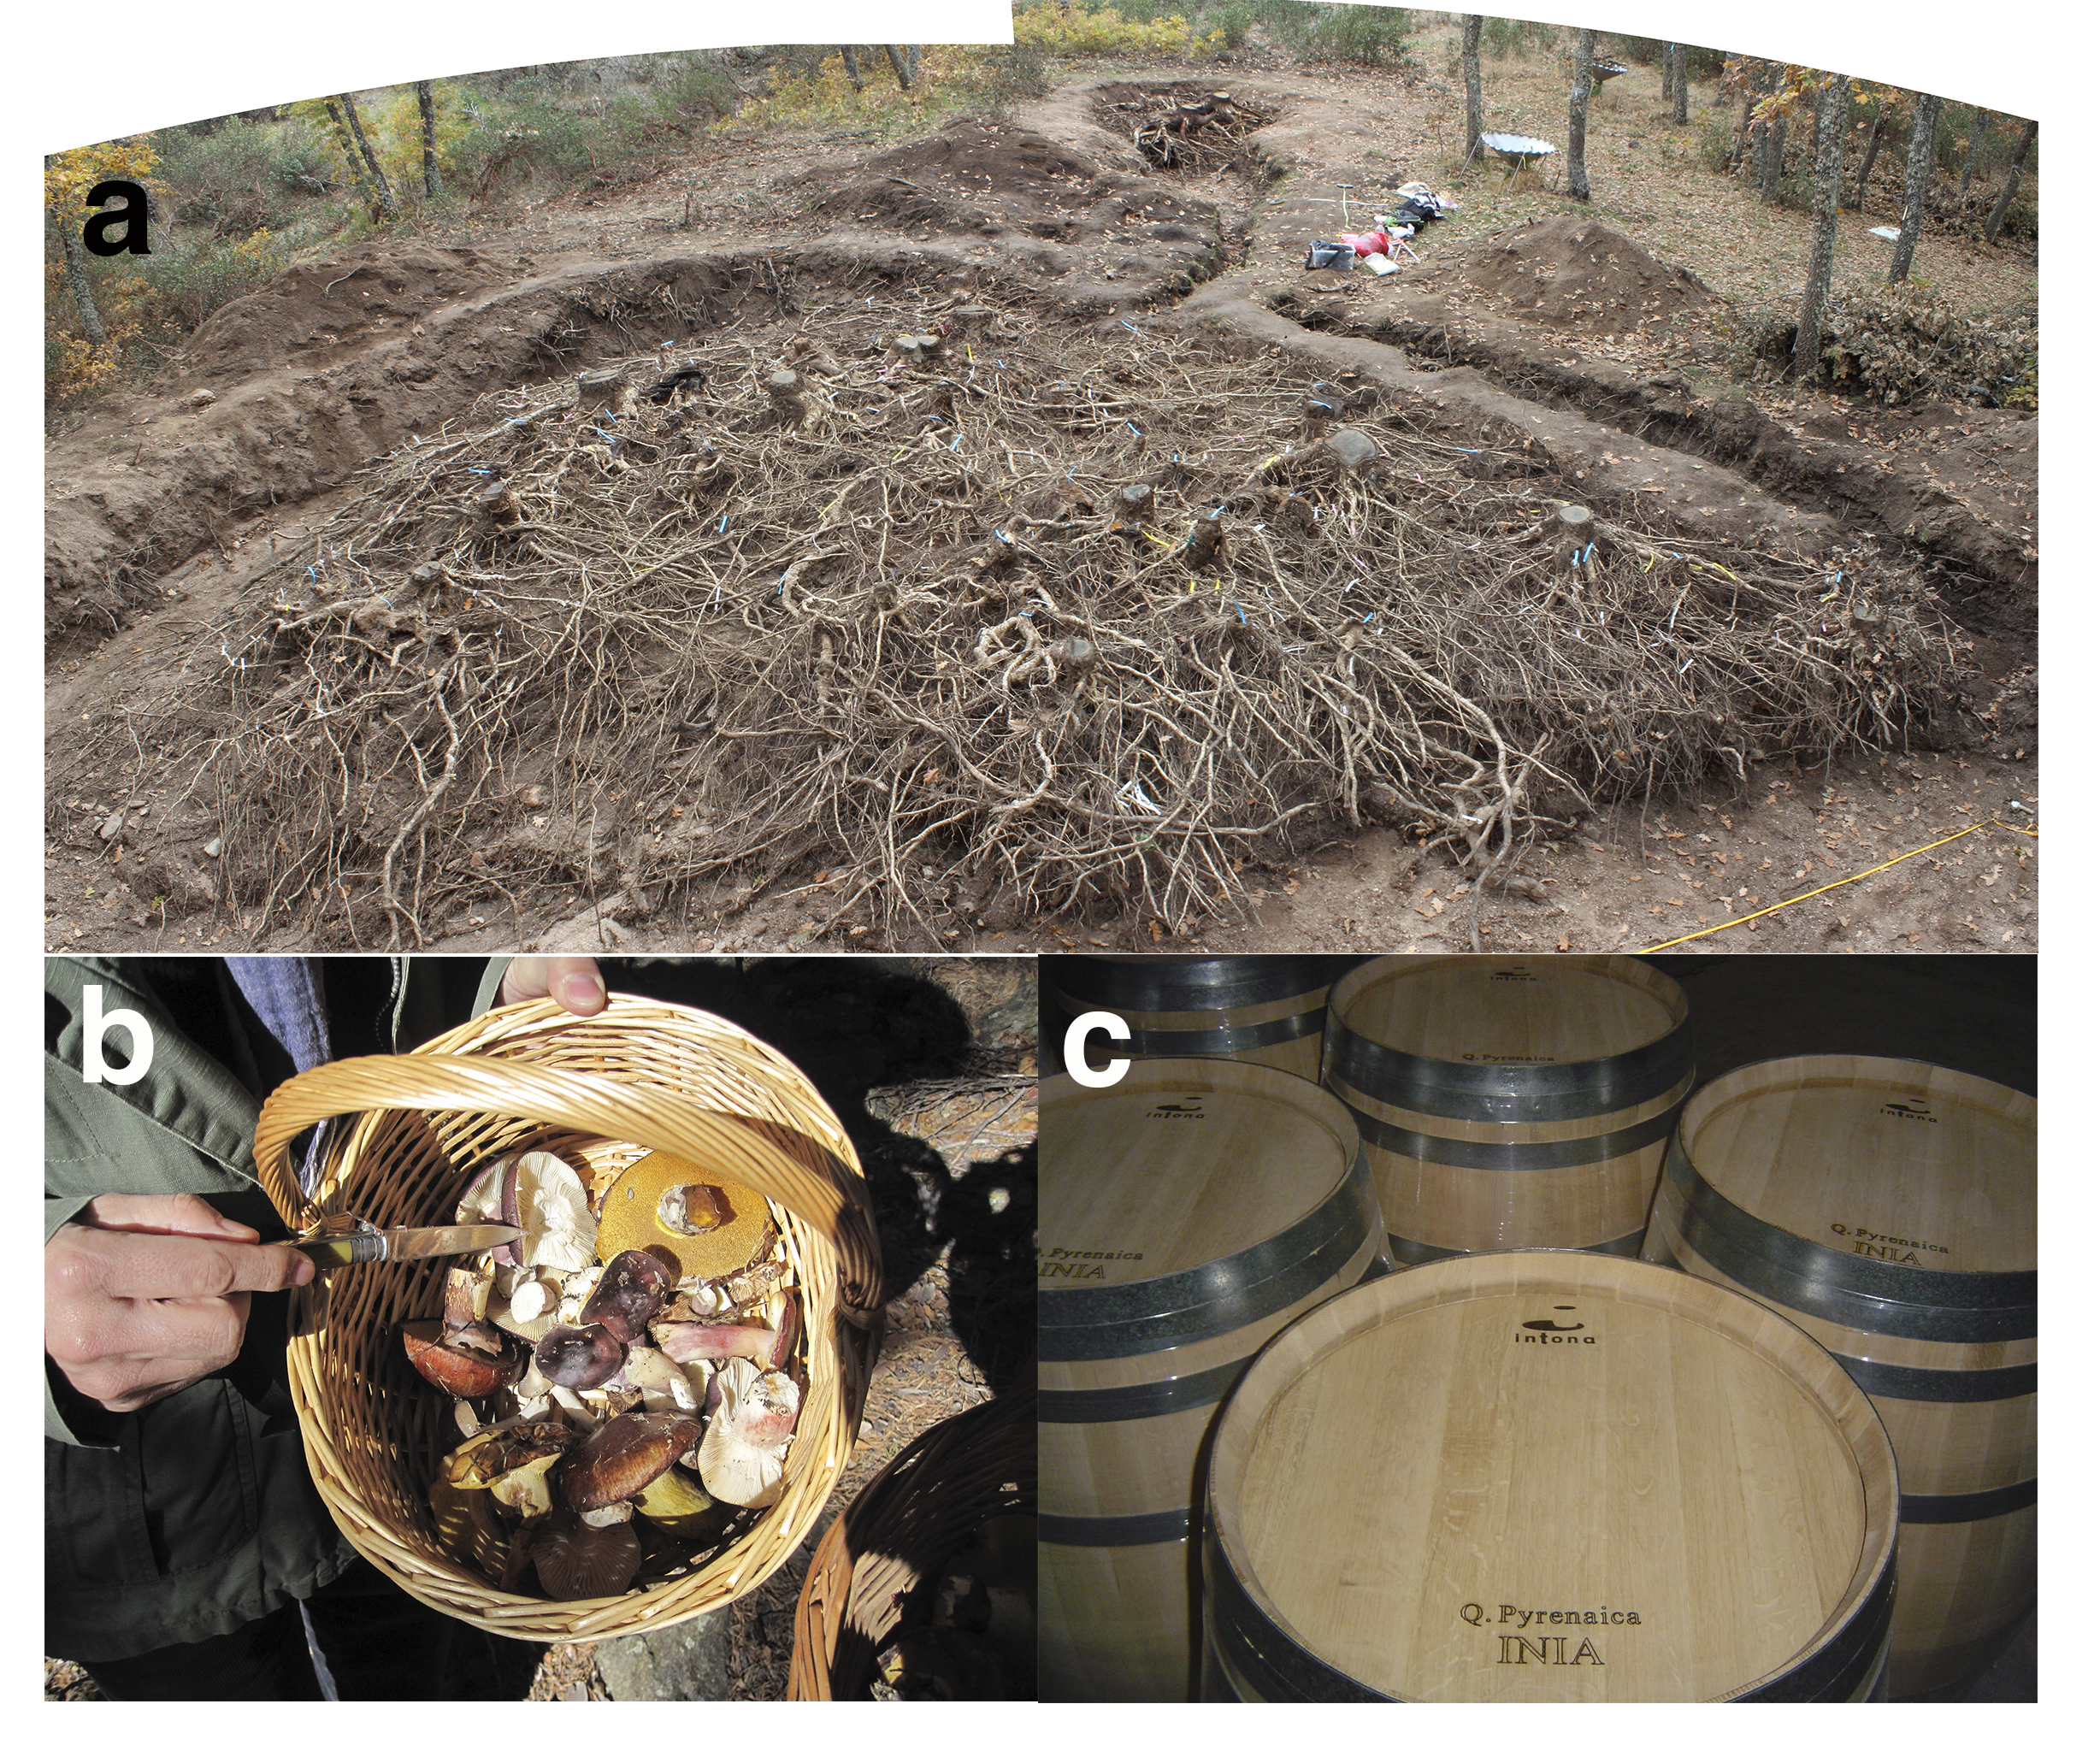
\includegraphics[height=12cm]{img/es/es-fig_3_composition.jpg}
    \caption{\textbf{(a)} Structure of the complex root system of several specimens of \Qp. \textbf{(b)} Melojo oak barrels for wine aging. \textbf{(c)} Collection of wild fungi in the surroundings of Robledal de Cáñar. Pictures from R. Salomón (a), A.J. Pérez-Luque (b) and B. Fernández de Simón (c) }\label{fig:es:rootsfungi}
\end{figure}

\subsubsection{Timber and firewood}\label{sec:es:provision-timber}
The wood of \Qp has not been appreciated as much as that of other oaks for built, although it has been used to obtain firewood directly or for charcoal production \autocites{MontoyaMeson1979SituacionActual}. For instance, some of the oak populations of Sierra Nevada have been intensely historically exploited to obtain firewood \autocites[\emph{e.g.} Robledal de Cáñar,][]{ValbuenaCarabanaGil2013GeneticResilience,MorenoLlorcaetal2016HistoricalAnalysis}. In addition, other uses of timber have been documented in this mountain range, such as its use in mining in the northernwestern oak woodlands of Sierra Nevada ("Robledal de San Juan", Güejar-Sierra, Granada) where it was used for mine tunnels and furnaces, and also as firewood to melt the mineral \autocites{Titos1990}. All these intense exploitation of timber have altered structure of these forests \autocite{PerezLuqueetal2020LanduseLegacies}. Notwithstanding, since the 1970s, anthropogenic pressure has been reduced, which lead an increase of tree density, and also in the basal area and average tree size \autocite{GonzalezDiazetal2020BosquesEspanoles}. This general pattern, observed for most of the forests of the Iberian Peninsula \autocite{Astigarragaetal2020EvidenceNon,GonzalezDiazetal2020BosquesEspanoles}, has been also confirmed for melojo oak forests. Thus, using data from second and third Spanish NFI, \citet{PerezLuqueetal2021ManualGestion} (see also chapter \ref{sec:carbon}) assessed the temporal variation on tree biomass of the forests. This analysis showed a total increase of 19172 \mgha between the two campaigns, with most of the field plots showing an increase pattern on biomass (89\% of the plots). This increase could be considered an asset for local populations around the oak woodlands, who could use the forest for firewood extraction

\subsection{Cultural services}\label{sec:es:cultural}
\subsubsection{Recreational values}\label{sec:es:cultural-recreation}

Nature recreation represents a valuable ecosystem service that has a substantial economic value and contributes considerably to income and employment of local communities \autocites{Schagneretal2017MonitoringRecreation}. Monitoring visitors to natural areas have been used often to estimate their recreational values in many areas \autocites{Schagneretal2017MonitoringRecreation}. We used this type of data obtained directly from pyroelectric sensors located in places within Sierra Nevada Protected Area to monitor visitors to this mountain range. We selected two singular oak woodlands of Sierra Nevada for which data are available: Dehesa del Camarate, popularly known as "Bosque Encantado" (Enchanted Forests), and Vereda de la Estrella. We compared the visits in the two oak woodlands with total visitors registered for all sensors installed in this mountain range during a year (n = 14; October 2018 to October 2019). Preliminary results showed that those two oak woodlands have a high number of visits (41145 visitors representing 37.36\% of total of annual visitors registered), particularly during autumn season, when they represent almost the total number of visits (\figref{fig:es:visitorsprofile}). 

\subsubsection{Recreational sports activities}\label{sec:es:cultural-sports}
One way to analyze the physical use of the landscape, and therefore its value as a provider of this cultural service, consists of quantifying the recreational activities performed in nature \autocites[\emph{e.g.}][]{RocesDiazetal2018AssessingDistribution}. We used the density of routes (hiking, biking, running and other types of outdoor activities) existing in the Wikiloc portal (www.wikiloc.com) (data query in January 2020) for all the municipalities belonging to the Sierra Nevada Natural Protected Area. For each municipality, the total number of routes, and their density (number of routes / surface area of the municipality in ha) were calculated. Each of the oak populations of Sierra Nevada were assigned to the municipalities in which they are present. Of the 47998 routes obtained for the Sierra Nevada mountain range, 49.94\% were in the 14 municipalities where oak woodland are present (Figure \ref{fig:es:socwikiloc}b). The density of routes in these municipalities ranged from 5.24 – 41.8 routes km$^{-2}$  (\tabref{tab:es:wikiloc}) being for most of them much higher than the average density of routes of the Sierra Nevada municipalities (17.88 routes km$^{-2}$).

\begin{figure}
    \centering
    \includegraphics[width=0.9\textwidth]{img/es/es-visitorsprofile.pdf}\caption{Evolution of the visitors numbers in two oak woodlands, \emph{Dehesa del Camarate} (green), and \emph{Vereda de la Estrella} (blue), comparing with the total of Sierra Nevada (gray). Data come from automatic counters (pyroelectric sensors) located at different points in the Sierra Nevada.}\label{fig:es:visitorsprofile}
\end{figure}

\subsubsection{Scientific knowledge}\label{sec:es:cultural-scientific} 
We used two indicators describing research activities to show the relevance of melojo woodlands regarding this ES. Firstly, we explored the spatial pattern of these activities in Sierra Nevada during the period 2009-2013 \autocites{Zamoraetal2017MonitoringGlobal}. For this, we used a database compiling the research authorization documents for the Sierra Nevada Protected Area to generate a density map with the hotspots areas of research activities for this area. Then we extracted the information for the oak populations. Most of the research authorizations are concentrated in the western side of the Sierra Nevada (Figure \ref{fig:es:scientific}b) particularly in the high summits area. The mean values of research permissions for \Qp oak woodlands in the period studied was 3.03 ± 0.06, with Genil and Cáñar oak populations (northwestern and southern oak populations respectively, contains the high concentration of research requests (Figure \ref{fig:es:scientific}b). Secondly, we created a density map of sampling protocols deployed in the Sierra Nevada \autocites{Zamoraetal2017MonitoringGlobal} using data from Sierra Nevada Global Change Observatory \autocites{Zamoraetal2016GlobalChange}. All the social-ecological monitoring protocols within this initiative were geolocated to generate a concentration map of sampling protocols by applying geostatistical hotspot detection techniques (Kernel density estimation)\autocites{Zamoraetal2016GlobalChange} (Figure \ref{fig:es:scientific}a). The results showed that the melojo oak woodlands are located in areas of high density of scientific activity (both sampling protocol density and research requested areas) in comparison with the other forest ecosystems of the Sierra Nevada.

\begin{figure}
    \centering
    \includegraphics[width=\textwidth]{img/es/es-scientific.pdf}
    \caption{Spatial localization of the research authorizations (Number of research authorizations) performed in Sierra Nevada in the period 2009-2015 (\textbf{a}); and map of density (scaled density) of socioecological monitoring protocols carried out in Sierra Nevada since 2008 (\textbf{b}). For both maps the spatial bounding boxes of each oak population are shown. Drawn from \autocites{Zamoraetal2017MonitoringGlobal,Zamoraetal2016GlobalChange}}\label{fig:es:scientific}
\end{figure}

\subsubsection{Aesthetic values}\label{sec:es:cultural-aesthetic} 
To explore the aesthetical values of these forests, we used data from \citet{MorenoLlorcaetal2020EvaluatingTourist}) who assessed a series of cultural services in Sierra Nevada by using data from the Flickr platform (www.flickr.com). These authors analysed a total number of 778 photographs and 18 they geolocated in \Qp woodlands (Figure \ref{fig:es:socwikiloc}c). Although this value is low with respect to the total number, it may be due to the fact that the highest density of photos in the analyzed dataset is located around the ski resort, at high altitude areas, and at village areas (mainly the Alpujarras) \autocites{RosCandeiraetal2020SocialMedia}. If we analyse forest separately (\emph{i.e.} native pine, holm oak, melojo oak forests, and pine plantations), the photos taken in melojo oak woodlands represent 32\% of the total.

\subsubsection{Singular trees}\label{sec:es:cultural-trees} 

Singular, large and/or monumental trees, in addition to perform key ecological functions \autocites[\emph{e.g.} nutrient cycling; support complex assemblages of species,][]{LindenmayerLaurance2017EcologyDistribution}, are creditors of natural value \emph{perse} \autocites{Asciutoetal2016MonumentalTrees}. They are considered part of a social realm, providing numerous socio-cultural benefits to society \autocites{BlicharskaMikusinski2014IncorporatingSocial,MoyaMoya2013MonumentalTrees}. Singular trees provide humans with aesthetic, symbolic, religious and historical values \autocites{BlicharskaMikusinski2014IncorporatingSocial}. They can be considered as singular trees by their age, dasometric (height, diameter at breast height), and socio-cultural (\emph{e.g.} surrounding landscape, local myths, legends and traditions, witnessing historical events) characteristics, so their conservation could contribute to the protection of both ecological and also social values \autocites{BlicharskaMikusinski2014IncorporatingSocial}. There are several individuals of \Qp in the study area, located in Busquístar (Alpujarras, southern slopes of Sierra Nevada), considered singular and/or monumental because of their extraordinary dimensions \autocite{IruritaFernandezetal2003ArbolesArboledas}, reaching tree heights of up to 19.5 meters and base perimeter of 6.7 meters. Likewise, there are some oak woodlands in Sierra Nevada that shelter specimens and/or singular populations of other species. For instance, the "Abedular del Barranco de los Alisos", located in the Dúrcal oak woodland \autocites{MartinezLabargaetal1990AbedularRelictico}. It is a small grove of about 300 individuals of birch (\emph{Betula pendula} subsp. \emph{fontqueri}) with an average height of 12 m. Other examples are the grove of birch trees located at the "Barranco de los Alisos", in the Dúrcal melojo population; or the Aliseda de la Cueva del Santo, where there are more than 100 alders (\emph{Alnus glutinosa}) accompanied by melojo oak and chestnut trees. In Andalusia region, there are also other melojo stands catalogued as singular, such as those located in the Sierra del Aljibe (Alcalá de los Gazules, southern Iberian Peninsula), whose specimens do not stand out for their dimensions but their location is unique and of great interest, representing a southern limit of distribution of the species \autocite{SanchezGarciaetal2003ArbolesArboledas}. 


\subsection{Spatial pattern for Ecosystem Services and ecosystem functioning of melojo forest of Sierra Nevada}\label{sec:es:spatial} 

\Qp populations in Sierra Nevada represent a rear-edge of the distribution of this oak species. Peripheral populations are usually considered more vulnerable compared with populations at the center of a species' range \autocite[\emph{i.e}. center-periphery hypothesis][]{Pirononetal2017GeographicVariation}. However, the expected lower performance and higher vulnerability for the peripherical populations do not always meet \autocite[\emph{e.g.}][]{Abelietal2014EffectsMarginality,Oldfatheretal2020RangeEdges,PerezLuqueetal2020LanduseLegacies}. For instance, several studies analyzed the evolution of productivity of melojo oak forests using vegetation indices derived from remote sensing (\emph{e.g.} Enhanced Vegetation Index, EVI), and found that Sierra Nevada melojo forests, despite their high seasonality, are the most productive ecosystems in Sierra Nevada \autocites{Dionisioetal2012SatelliteBasedMonitoring,AlcarazSeguraetal2016ChangesVegetation,PerezLuqueetal2015OntologicalSystem,Cazorlaetal2020RemoteSensingbased}. These forests also showed a positive trend in productivity since 2000, highlighting their importance in carbon gain and therefore as carbon sinks \autocite{PerezLuqueetal2015OntologicalSystem} despite their expected low performance. 

The quantification of some ES provided by melojo oak populations in Sierra Nevada, allows us to compare the supply of ES among those populations, and to describe what ES category predominate for each of the oak population cluster’s in this mountain range (\tabref{tab:es:oak-cluster}). This also allows us to explore the spatial pattern of ES supply by the melojo oak forest. Regarding the regulating services evaluated, we observed that the southern populations have higher values for carbon sequestration potential, mean EVI and soil organic carbon than for the other clusters (\figref{fig:es:oak-compare}), despite the theoretically greater vulnerability due to their location in the southernmost areas of Sierra Nevada. For cultural services, the NW populations present high values for sports activities, number of visitors, and density of sampling protocols (scientific value). Finally, for provisioning and support services we observed a variable pattern depending on the service evaluated.

\begin{figure}
    \centering
    \includegraphics[width=\textwidth]{img/es/es-plotSN.pdf}\caption{Comparison of ecosystem services (cultural: yellow; regulation: blue; supporting: gray) for oak populations cluster identified in Sierra Nevada. See \tabref{tab:es:oak-cluster} for a detailed description 
}\label{fig:es:oak-compare}
\end{figure}

\subsection{Temporal evolution of Ecosystem Services provision within \Qp forests in Sierra Nevada}\label{sec:es:temporal} 
Analyzing the temporal change of ES is key to understand how human societies have been using natural resources in different time periods. Besides, this approach helps us to understand the temporal trade-offs among ES. We compiled datasets of several ES indicators for which long temporal series were available (\tabref{tab:es:temporal}). Those data were available mainly for one of the oak woodlands (Robledal de Cáñar) located on the southern slope of Sierra Nevada (CAÑ, Figure \ref{fig:es:location}b). 

Both overuse and abandonment of melojo woodlands provide very different scenarios for the provision of ES and for the socioeconomic demand for them. From ancient (not determined) times until the period 1960-1970 there was an intense use of the resources provided by the oak forests. Local inhabitants used firewood from the forests for charcoal and fuel, reflected by the lower oak-tree density of the forests. Oak acorns were harvested for livestock feed (mainly pigs), as reflected in the auction records of the public forests. Therefore, many forest patches were cleared to create pastures for livestock and mountain crops, which explains the lower amount of forest area. In this period, provisioning ES prevailed over the regulating (poorly considered) or the cultural (not considered). Afterwards, due to changes in socio-economic conditions, a process of depopulation of rural areas (rural exodus) began, resulting in the abandonment of traditional activities as were reflected by several indicators (\figref{fig:es:temporal}). For instance, a decrease in the number of sheep (at least since 1956) and beekeeping (at least since 1980). This pattern also shows that provision ES of \Qp forests tend to be less important in Sierra Nevada. It is consistent with other land uses not shown in the graph due to the lack of quantitative data (\emph{e.g.}, wood extraction, extent of agriculture within the forest, etc.). This behavior means, in terms of ES, that there is a trend towards less intense use of some provisioning services in melojo forests in Sierra Nevada. This decrease in the indicators related to provisioning ES coincides with an increase of the area occupied by melojo forests, and a gradual increase in their tree density (both at least since the end of 1950s). This pattern is also reflected in the forest’s primary production (at least since 2000) as EVI temporal series shown (\figref{fig:es:temporal}). Consequently, increased forest productivity is also reflected in a raise in aboveground forest biomass. The consequences in terms of ES, is a reduction of the provisioning services as opposed to an increase in regulating services, mainly due to a recovery of the forest following the almost complete abandonment of traditional activities. On the other hand, after the declaration of Sierra Nevada as natural protected area (1989), there was an increase in the supply of cultural ES, as reflected for example in the increase in the number of visitors (\figref{fig:es:temporal}). The underlying pattern that seems to explain the above-describe trends is also shown in \figref{fig:es:temporal}: the steady and consistent decrease in human population since at least 1960. Our study area has suffered a strong drainage in human population mainly due to the migration to big cities. This demographical pattern could explain the observed decrease in the use of provisioning services, as well as the increase in their production (due to the land abandonment). Besides, the increase in the interest of melojo forests by visitors is also compatible with this demographic situation: the currently more urban people enjoy visiting natural areas during their spare time. 

\begin{sidewaysfigure}
    \centering
    \includegraphics[width=.8\textwidth]{img/es/es-temporal_evolution_modified_v1.pdf}
    \caption{Temporal evolution of indicators of ES supply by \Qp woodlands in Sierra Nevada. See \tabref{tab:es:temporal} for description of the sources. All data referred to Robledal de Cáñar oak woodland (southern slope of Sierra Nevada), except visitors numbers corresponding to all Sierra Nevada Protected Area.}\label{fig:es:temporal}
\end{sidewaysfigure}

Using the sequence of trends described above, we can infer a temporal evolution of the ES provided by melojo forests in Sierra Nevada (\figref{fig:es:schema}). During the first half of XX\textsuperscript{th} century, human activity was intense in our study area. This means that the most relevant ES were those related with the provision of goods (\emph{e.g.}, timber, grassland, crops, etc.). This situation implied an intense use of land that sometimes could threatened some regulating ES (\emph{e.g.}, soil protection, habitat for endangered species, etc.). During the 1950-60s, the situation changed: due to changes in the macroeconomical situation, an intense migration process began to shift population from rural areas to big cities. This involved the abandonment of previous land use and therefore the underutilization of provisioning ES. The creation of two overlapping protected areas (Natural Park in 1989 and National Park in 1999) reinforced this trend by discouraging intense human activities in the area. The reduction in the intensity of use and therefore the decline of  provisioning ES could have fostered a process of secondary succession in the melojo forests. This implied the recovery of many regulating ES such as soil or habitat protection. In the transition from overexploitation to abandonment of the oak forest, many ecosystem services linked to the functioning of an increasingly biodiverse and complex forest ecosystem are being favored. However, in some cases a tradeoff is attained in relation to ecosystem services such as carbon storage. For example, increased forest encroachment implies higher aboveground carbon storage but also higher risk of severe wildfires and therefore carbon losses. Finally, once Spain became a world class tourism attraction (from 2000 onwards), the most relevant ES in our zone are those cultural related to leisure activities.

\section{Concluding remarks}\label{sec:es:concluding} 

In this work we combined a literature review with expert criterion to identify and to characterize the main ecosystem services provide by \Qp woodlands. The literature review revealed the existence of many works related to wine ageing, highlighting the potential of this species for wine production (\tabref{tab:es-review}). Interestingly, this ES has not been identified in our local scale search. It is also remarkable that no work has been found in our literature review that evaluates cultural services in these forests. However, this pattern changes when the ecosystem services are analyzed in more detail as in our case study. Thus, the combination of expert criteria with data at a more local scale allowed us to highlight the existence of diverse cultural ecosystem services provided by these forests. 

Our compilation of local scale data has allowed us to quantify many of these ES, which on the one hand highlights the relevance of these forest formations, and on the other hand, provides to natural resource managers with more information and tools to help them in the decision-making process. Because melojo forest is a human-shaped ecosystem, management is required to guide their development \autocite{Hobbsetal2006NovelEcosystems}. How we manage this new ecosystem effectively is a point for debate. In this sense, incorporating information on ecosystem services can significantly help managers to make decisions due to its integrative and interdisciplinary nature. Our study also adds some interesting insights for the study of ES provided by forests. For instance, we observed a highly variable temporal pattern of some ES, such as the recreational values. Some melojo woodlands of Sierra Nevada concentrate a large part of the visitors recorded in the Sierra Nevada Natural Area (\figref{fig:es:visitorsprofile}) during a specific time period. This highlights the need to consider the temporal dimension of the ES evaluated, and to pay attention to the pressure that these ecosystems may be suffering temporarily due to the high number of visitors. Therefore, from a natural resource management point of view, it is necessary not only to analyze the ES provided by an ecosystem, but also we would consider the spatio-temporal pattern of the ES supply. In this sense, it would be interesting to carry out detailed studies to provide managers with a comprehensive assessment of the possible impacts of visitors.

Another relevant outcome is the differences identified within melojo forests regarding their capacity to provide ES. We observed that southern populations seem to be able to sequester more carbon than northern ones. Besides, northwestern populations are specifically valuable for the cultural services that they provide. The main conclusion regarding these facts is that we need to specifically assess the capacity of ES provision at a local scale. Only by doing so, we would be able to quantify the provision of ES considering the specific biophysical features of each target area. 

Finally, we have assessed the change in ES provision patterns across time of this forest system with high conservation values. Both ancient overuse and current abandonment of melojo woodlands provided contrasting scenarios for the provision of ES and for the socioeconomic demand for them in Sierra Nevada. Although the history of land use patterns in our target area is well known, we have described that history using the framework of ES. We observed how the land use could modified the temporal provision of the ES in the melojo forests.

All these results provide enough evidence for us to advocate for the promotion of local scale studies like this one. The combination of literature research with analysis of local long term series and with detailed understanding of the target populations, has allowed us to unveil ES patterns that otherwise would have been kept hidden. Besides, thanks to the existence of the ES conceptual framework, our results can be easily compared with other studies done in other areas. Thus, we conclude that local scale studies can be a good way to gather information on ES supply both at a local and at larger scales. 

\begin{sidewaystable}
\caption{Quantification of several Ecosystem Services (ES) for Sierra Nevada oak population clusters \autocites[see][]{PerezLuqueetal2021EcologicalDiversity}. N: Northern populations, NW: Northwestern populations; S: Southern populations.}\label{tab:es:oak-cluster}
\centering
\scriptsize
\resizebox{\linewidth}{!}{%
\begin{tabular}{>{\hspace{0pt}}m{0.14\linewidth}>{\hspace{0pt}}m{0.402\linewidth}>{\hspace{0pt}}m{0.158\linewidth}>{\centering\hspace{0pt}}m{0.075\linewidth}>{\centering\hspace{0pt}}m{0.085\linewidth}>{\centering\arraybackslash\hspace{0pt}}m{0.077\linewidth}} 
\toprule
\textbf{ES Indicator} & \textbf{Definition} & \textbf{Units} & \textbf{N} & \textbf{NW} & \textbf{S} \\
Plant richness & Mean richness of plant species recorded in forest invetories & Species number & 58 & 33.5 ± 1.04 & 33.5 ± 6.69 \\
Passerine bird richness & Mean richness of passerine birds recorded at bird censuses on oak woodlands & Species number & 55 & 58.5 ± 0.5 & 48 \\
Genetic diversity & Density of genotypes represented by one stem (unique genotypes, GU) per hecatera & Genotypes Uniques ha$^{-1}$ & 60 &  & 107.5 ± 27.5 \\
Genetic diversity & Density of multilocus lineages (MLL) per hectarea & Multiloculs Lineages ha$^{-1}$ & 89 &  & 191 ± 60 \\
Biomass increment & Increment of Biomass amount (Growth rate) between two National Forest Inventories (SNFI2 and SNFI3) & Mg Biomass ha$^{-1}$ year$^{-1}$  &  & 0.214 ± 0.136 & 0.18 ± 0.053 \\
Recreational values & Percentage of visits (visits registered in the oak woodland / total visits registered in Sierra Nevada) & \% & 16.69 & 20.68 &  \\
Sport activities (total routes) & Mean of total routes registered at Wikilock in the Municipalities where oak woodlands are located & Sport activites & 1170 & 2367.5 ± 520.36 & 1318 ± 489.95 \\
Scientific research authorizations & Average values of the Kerneld Density Estimate of the research permissions & Number of autorization research &  & 2.61 ± 0.09 & 3.34 ± 0.1 \\
Scientific sampling density & Average of Normalized Kernel Density Estimation of the Density of Monitoring methodologies & scaled value (0-100) & 22.94 ± 1.07 & 45.56 ± 1.52 & 19.57 ± 0.59 \\
EVI mean & Average of annual EVI mean for all pixels covering oak woodlands populations (period 2000-2018) &  & 0.257 ± 0.003 & 0.256 ± 0.004 & 0.275 ± 0.003 \\
Potential Carbon sequestration & Aveage values of the CO$_2$ potential sequestration & Mg CO$_2$ ha$^{-1}$ & 265.07 ± 1.41 & 256.72 ± 1.05 & 273.91 ± 0.93 \\
SOC & Average values of the mean Soil organic content at a 0-30 cm depth & Mg SOC ha$^{-1}$ & 51.27 ± 0.29 & 52.59 ± 0.34 & 55.11 ± 0.33 \\
\bottomrule
\end{tabular}
}
\end{sidewaystable}

\begin{sidewaysfigure}
\centering
    \includegraphics[width=.8\textwidth]{img/es/es-schema.pdf}
    \caption{\textbf{(a)} Temporal evolution of anthropic uses associated with Sierra Nevada oak forests, and their effect on the provision of ecosystem services \textbf{(b)}. For each category of ecosystem services, an estimate of the supply at each time point is shown.}\label{fig:es:schema}
\end{sidewaysfigure} 

\renewcommand{\partname}{Parte}
\part{Discusión General}
%\part{Additional Example Part}
% !TEX root = ../my-thesis.tex
%
\selectlanguage{spanish}
\chapter{\textcolor{ctcolormain}{Discusión General}}\label{sec:discussions}
\newpage

\subsection*{Diversidad ecológica dentro del borde posterior de distribución de \Qp. }\label{sec:discussions:diversidad}

La distribución de \Qp está condicionada por el periodo de sequía estival, necesitando un mínimo de 100-150 mm de precipitación estival para su supervivencia \autocite{BlancoCastroetal2005BosquesIbericos,GarciaJimenez20099230Robledales}. Varios autores han señalado la importancia de los índices pluviométricos y ombrotérmicos en la separación entre bosques templados y mediterráneos para esta especie a lo largo de su área de distribución \autocite{delRioetal2007BioclimaticAnalysis}. A escalas más detalladas, la distribución de esta especie se rige por un complejo gradiente relacionado con la temperatura, la precipitación y la radiación \autocites{Gavilanetal2007ModellingCurrent,Urbietaetal2011MediterraneanPine}. En el capítulo \ref{sec:multivar}, hemos encontrado que la precipitación estival y anual son factores muy importantes para explicar la distribución de los bosques de \Qp en Sierra Nevada. De hecho, hemos observado diferentes grupos de poblaciones de \Qp en esta región montañosa discriminados principalmente por la precipitación y la radiación. Los robledales situados al norte y al noroeste, se localizan en fondos de valle con orientaciones norte, donde la humedad relativa es mayor como consecuencia de una menor radiación solar. Por otro lado, las poblaciones de la vertiente sur de Sierra Nevada reciben un aporte extra de agua procedente del aire húmedo del mar \autocite{MartinezParrasMoleroMesa1982EcologiaFitosociologia}. Las diferencias en la disponibilidad de agua entre las poblaciones de robles podrían afectar a varios procesos ecológicos como la germinación y supervivencia de las plántulas \autocites{Gomez2003ImpactVertebrate, GomezAparicioetal2008OakSeedling,Mendozaetal2009SeedingExperiment}, así como a la regeneración de la especie \autocites{Gomezetal2001ProblemasRegeneracion}, debido principalmente al papel clave de la disponibilidad de agua a escala de micrositio, que facilitan la germinación y el establecimiento de las plántulas. Asimismo, como se ha observado para otras especies de \emph{Quercus} \autocites[\emph{e.g.}][]{Tessieretal1994DeciduousQuercus,DiFilippoetal2010ClimateChange,GeaIzquierdoetal2011TreeringsReflect,GarciaGonzalezSoutoHerrero2017EarlywoodVessel}, la disponibilidad de agua es uno de los principales factores limitantes que afectan al crecimiento secundario de \Qp (ver resultados obtenidos en el capítulo \ref{sec:dendro}). 

Las poblaciones de \Qp situadas en Sierra Nevada, que representan un borde posterior (\emph{rear-edge}), no son ecológicamente homogéneas, ni en sus condiciones ambientales ni en su composición de especies. Al explorar las características de las poblaciones de roble melojo en Sierra Nevada, hemos observado la existencia de grupos separados de poblaciones basándonos en sus características ambientales, siendo la radiación y la precipitación las principales variables discriminantes (ver capítulo \ref{sec:multivar}). Esta heterogeneidad va en la línea de otros estudios que señalan una dinámica ecológica diferencial para estos bosques en Sierra Nevada. Así por ejemplo, la productividad primaria de estos ecosistemas (medida mediante el uso de teledetección) difiere entre las poblaciones de \Qp de Sierra Nevada, con los robledales de la vertiente sur mostrando un mayor verdor anual de la vegetación que los de la vertiente norte \autocites[ver capítulo \ref{sec:onto} ][]{Dionisioetal2012SatelliteBasedMonitoring,PerezLuqueetal2015OntologicalSystem,PerezLuqueetal2020LanduseLegacies}. Asimismo, otros estudios encontraron diferencias en la dinámica estacional del verdor \autocite{Dionisioetal2012SatelliteBasedMonitoring}, y en la tendencia temporal de la productividad primaria \autocites{PerezLuqueetal2015OntologicalSystem,AlcarazSeguraetal2016ChangesVegetation}, esto último parece estar relacionado con la diferente tendencia observada para la cubierta de nieve en las vertientes norte y sur de Sierra Nevada (ver capítulo \ref{sec:onto}).  

Curiosamente, también hemos encontrado diferencias en la diversidad de especies entre los grupos de poblaciones derivadas de la agrupación basada en variables ambientales (ver capítulo \ref{sec:multivar}). Estos resultados son consistentes con los aportados por \textcite{Loriteetal2008PhytosociologicalReview}, que señalaron que las diferencias observadas para el componente florístico en las poblaciones de \Qp de Sierra Nevada están relacionadas con las condiciones microclimáticas. En este sentido, los robledales situados en el norte de Sierra Nevada presentan mayor similitud florística con los situados en el centro de la distribución de \Qp que con los que se localizan en la vertiente sur de Sierra Nevada (geográficamente más cercanos) \autocites{Loriteetal2008PhytosociologicalReview}. Además de los factores climáticos, las diferencias florísticas entre las poblaciones de \Qp en Sierra Nevada también podrían estar relacionadas con el impacto antropogénico sufrido, ya que las perturbaciones antrópicas pueden afectar a los patrones florísticos, como se ha documentado para los robledales del centro de la Península Ibérica \autocite{Gavilanetal2000EffectsDisturbance}. Por ejemplo, el robledal del Camarate (que representa el grupo de población Norte en Sierra Nevada, ver capítulo \ref{sec:multivar}) mostró una mayor diversidad y riqueza de especies vegetales, lo que puede estar relacionado con un mejor estado de conservación, ya que esta población ha estado menos expuesta a la intensa actividad antropogénica \autocite{JimenezOlivencia1991PaisajesSierra}. Por el contrario, las poblaciones de robledal situadas en la vertiente sur, mostraron una composición florística más pobre condicionada tanto por el clima como por el intenso uso del suelo \autocite{CamachoOlmedoetal2002DinamicaEvolutiva,AlAallalietal1998EstudioVegetacion}. Por tanto, podemos atrevernos a afirmar la importancia del uso del suelo para entender el estado actual de los robledales de \Qp dentro del borde posterior de su distribución. 

La notable coincidencia entre la agrupación de las poblaciones derivada del análisis de las variables ambientales y la ordenación de las poblaciones según la composición de especies, sugieren una relación entre la heterogeneidad de los factores ambientales y la variabilidad de la composición de especies para estos bosques. Esta diversidad de condiciones ecológicas para las poblaciones de \Qp situadas en este borde posterior, está en consonancia con los altos niveles de diversidad genética mostrados por las poblaciones de esta especie en Sierra Nevada \autocites{ValbuenaCarabanaGil2013GeneticResilience, ValbuenaCarabanaGil2017CentenaryCoppicing}. La heterogeneidad climática y topográfica que existe en Sierra Nevada ofrece una gran diversidad de microhábitats, lo que ha permitido que esta región montañosa actúe como refugio de diferentes especies \autocites{MedailDiadema2009GlacialRefugia, GomezLunt2007RefugiaRefugia,BlancoPastoretal2019TopographyExplains}, incluso para las especies de \emph{Quercus} caducifolios durante el último periodo glacial \autocites{Breweretal2002SpreadDeciduous, Olaldeetal2002WhiteOaks,RodriguezSanchezetal2010TreeRange}. De hecho, existen evidencias fósiles y genéticas que sugieren que diferentes especies de \emph{Quercus} sólo sobrevivieron en refugios del sur durante el último máximo glacial \autocite{Breweretal2002SpreadDeciduous,Petitetal2002IdentificationRefugia,BhagwatWillis2008SpeciesPersistence,BirksWillis2008AlpinesTrees}. La persistencia en un refugio sugiere una combinación de un entorno local moderadamente adecuado que amortigua el clima regional, y una relativa tolerancia al cambio climático, ya sea por una pronunciada plasticidad fenotípica, y/o por la capacidad de adaptación \autocites{Gavinetal2014ClimateRefugia}. Este podría ser muy bien el caso de \Qp, una especie que alberga una alta diversidad genética \autocite{ValbuenaCarabanaGil2013GeneticResilience}, situada en una región montañosa con una topografía compleja que podría proteger a las poblaciones locales contra los rápidos cambios climáticos y permitir que las especies persistan a pesar de los entornos regionales desfavorables.

La identificación de diferentes grupos de poblaciones en función de las variables ambientales a escala de detalle (ver capítulo \ref{sec:multivar}), es importante a la hora de modelizar la distribución de una especie y prever los impactos del cambio global sobre ella, ya que los factores que controlan la distribución de las especies pueden variar en función de la escala de observación \autocites{GuisanThuiller2005PredictingSpecies,Urbietaetal2008SoilWater,SanchezdeDiosetal2009PresentFuture}. Los resultados que hemos obtenido en el capítulo \ref{sec:multivar}, que indican una separación de poblaciones de \Qp en función de la disponibilidad de agua, sugieren la necesidad de incorporar estos resultados en los modelos de predicción del impacto de cambio climático sobre esta especie.  Incorporar las adaptaciones locales de las poblaciones en los modelos predictivos, puede ayudar a evitar representaciones erróneas del desplazamiento del área de distribución de las especies bajo condiciones climáticas cambiantes \autocite{BenitoGarzonetal2011IntraspecificVariability}. Esto es especialmente importante en el caso de las especies con bordes posteriores situados en regiones de montaña, ya que estas zonas ofrecen una amplia diversidad de microhábitats debido a la heterogeneidad climática y topográfica \autocite{MedailDiadema2009GlacialRefugia}.
Por ejemplo, algunos trabajos recientes han realizado modelos de alta resolución de la distribución de especies arbóreas relictas en montañas Mediterráneas del sur (\emph{e.g}. \emph{Abies pinsapo, Pinus sylvetris} y \emph{P. nigra}) proporcionando información útil para las acciones de gestión forestal \autocite{LopezTiradoHidalgo2014HighResolution}.

\subsection*{Los robledales de \Qp en Sierra Nevada frente al cambio climático
}\label{sec:discussions:climate}

Varios son los trabajos que han documentando un aumento generalizado de las temperaturas, así como un cambio en los patrones de precipitación para la región Mediterránea \autocites[\emph{e.g.}][]{PerezBoscolo2010ClimateSpain,GarciaRuizetal2011MediterraneanWater,GiorgiLionello2008ClimateChange,Crameretal2020ClimateEnvironmental}. Estos patrones generales también han sido observados para Sierra Nevada, donde varios estudios, a partir de datos de estaciones meteorológicas y usando mapas climáticos de alta resolución, han encontrado tendencias positivas para las temperaturas mínimas y máximas anuales, así como un descenso generalizado en la precipitación desde 1960 \autocite{Benitoetal2014ClimateSimulations,PerezLuqueetal2016SenalesCambio,PerezLuqueetal2021ClimaNevadaBase,PerezPalazonetal2015ExtremeValues}. Esos cambios observados en las variables climáticas parecen afectar a varios procesos ecológicos, como por ejemplo la dinámica de la cubierta de nieve en ambientes de montaña \autocite{Trujilloetal2012ElevationdependentInfluence}. Así, en algunas montañas europeas se han registrado descensos significativos en la extensión y duración de la cubierta de nieve \autocite{Marty2008RegimeShift,MorenoRodriguezetal2005EvaluacionPreliminar,Nikolovaetal2013ChangesSnowfall,Scherreretal2004TrendsSwiss}. En Sierra Nevada, además de estos cambios, se han observado modificaciones en la fecha de inicio y de fusión de la cubierta de nieve \autocites{PerezLuqueetal2016SenalesCambio}. Específicamente se han documentado para los últimos 20 años un retraso en la fecha de inicio de la presencia de nieve, y un adelanto en la fecha de fusión de la nieve \autocites{PerezLuqueetal2016SenalesCambio}. Por ejemplo, para el 70\% de los píxeles que coinciden con la distribución de los robledales en Sierra Nevada, hemos encontrado tendencias hacia una fecha de deshielo mas temprana (ver capítulo \ref{sec:onto}). 

Las alteraciones en los patrones de disponibilidad hídrica, tal y como apuntábamos en los objetivos de esta memoria doctoral, pueden afectar al funcionamiento ecosistémico de los robledales en Sierra Nevada. Mediante el uso del sistema de ontologías (ver capítulo \ref{sec:onto}), hemos observado tendencias temporales significativas para el NDVI de verano en los robledales. En concreto, el 75\% de los píxeles que cubren los robledales han mostrado tendencias positivas significativas. El sistema de ontologías desarrollado, nos ha ayudado a desvelar la co-ocurrencia de tendencias significativas tanto en la cobertura de nieve (factor abiótico) como en el funcionamiento del ecosistema (NDVI). Por ejemplo, en las poblaciones de robledal situadas en la parte más occidental de Sierra Nevada, la mayor parte de sus píxeles muestran esta co-ocurrencia. Las implicaciones ecológicas de esta co-ocurrencia pueden explicarse argumentando que el deshielo más temprano proporciona agua a los árboles de \emph{Q. pyrenaica} cuando están en la mitad de su temporada de crecimiento. Este suministro de agua más temprano puede favorecer que los árboles sean más productivos en verano. Por otro lado, las poblaciones de robledal situadas en el sur de Sierra Nevada, también muestran esta co-ocurrencia en sentido contrario: la falta de tendencias significativas en la productividad de verano para ésta poblaciones, podría explicarse por la falta de píxeles con tendencias hacia un deshielo más temprano en estas zonas. Aunque estos resultados hay que considerarlos con cautela, parecen indicar la existencia de un vínculo entre el estado de un factor abiótico (duración de la cubierta de nieve) y el funcionamiento de los ecosistemas (productividad), tal y como ha sido documentado en otras regiones montañosas \autocite{Wanetal2014ChangeSnow,DyeTucker2003SeasonalityTrends}. Estos resultados pueden utilizarse en la programación de algunas actuaciones forestales de mejora de los robledales. Por ejemplo, si entre las actuaciones forestales se contemplara la realización de refuerzos poblacionales mediante plantación, éstas se pueden realizar en aquellas poblaciones donde se haya observado un patrón de mayor disponibilidad de agua, lo cual aumentaría la posibilidad de éxito de la actuación, teniendo en cuenta la importancia de la disponibilidad de agua para esta especie (ver capítulo \ref{sec:multivar}). 

En Sierra Nevada, al igual que en otras zonas del sur de Europa, se ha observado en los últimos años un aumento en la duración, frecuencia y severidad de los eventos de sequía \autocites[ver capítulo \ref{sec:dendro} y apéndice \ref{sec:appendix:dendro};][]{VicenteSerranoetal2014EvidenceIncreasing,Staggeetal2017ObservedDrought,Spinonietal2015EuropeanDrought,Pascoaetal2017DroughtTrends}, con una tendencia hacia veranos más secos \autocites{Spinonietal2017PanEuropeanSeasonal}. Esta situación está alterando el funcionamiento de los ecosistemas mediterráneos a diferentes escalas \autocites{Penuelasetal2017ImpactsGlobal,Forneretal2018ExtremeDroughts,Liuetal2020EffectsDecadal,OgayaPenuelas2021ClimateChange}, puesto que la sequía afecta a aspectos fisiológicos, funcionales, estructurales y demográficos de los ecosistemas forestales \autocites{Allenetal2010GlobalOverview, Assaletal2016SpatialTemporal}. No obstante, se están observando respuestas divergentes de los ecosistemas forestales a la sequía \autocites{Andereggetal2020DivergentForest}, poniendo de manifiesto la importancia de otros aspectos, como por ejemplo, el momento en el que ocurre la sequía \autocites{Huangetal2018DroughtTiming}. Esto es de especial relevancia para especies como \Qp que presenta una fenología de crecimiento bien marcada con su máximo de crecimiento en final de primavera y verano \autocites{PerezdeLisetal2016ChangesSpring}. 

Los eventos de sequía severa afectan a la dinámica de crecimiento de \Qp. Los resultados del capítulo \ref{sec:dendro} muestran claramente una reducción en el crecimiento primario (verdor medido usando EVI) y en el crecimiento secundario (BAI) para los eventos de sequía de 2005 y 2012. Asimismo, observamos que durante los eventos de sequía extrema, como la registrada en 1995, se produjo la mayor reducción del crecimiento radial. Ese evento de sequía causó graves y extensos daños en los ecosistemas Mediterráneos de la Península Ibérica \autocite{Penuelasetal2001SevereDrought,Gazoletal2018ForestResilience}. 

Las respuestas de los árboles a la sequía son dependientes del sitio \autocite{Babstetal2013SiteSpecies}, particularmente para las poblaciones situadas en su borde posterior de distribución \autocites{CavinJump2017HighestDrought,DoradoLinanetal2017LargescaleAtmospheric}. 
Tal y como hemos observado en el capítulo \ref{sec:dendro}, tanto el verdor de la vegetación (EVI), como el crecimiento secundario de los árboles (BAI), se vieron más afectados por los eventos de sequía en las poblaciones de robledal situadas en la cara norte de Sierra Nevada que las situadas en la cara sur. Específicamente, encontramos que las poblaciones situadas en la cara norte mostraron anomalías de EVI más negativas para la sequía de 2005 que las situadas en la cara sur. Asimismo, las correlaciones entre el crecimiento secundario de los árboles y el índice SPEI (tanto del año hidrológico como de verano) fueron más intensas para las poblaciones de la cara norte, lo cual se puede interpretar como una mayor sensibilidad a la sequía en los sitios más secos \autocite{GeaIzquierdoCanellas2014LocalClimate}. Por otro lado, es interesante destacar la gran variabilidad en respuesta al clima mostrada por las poblaciones de roble a lo largo de un estrecho gradiente. Por ejemplo, los árboles situados en las zonas altas del robledal de Cáñar mostraron un BAI superior a los situados en elevaciones más bajas, aunque ambos sitios de muestreo se encuentren muy cerca el uno del otro. 

No obstante, a pesar de los severos eventos de sequía de las últimas décadas, llama poderosamente la atención la tendencia positiva para el verdor de la vegetación mostrada por los bosques de \Qp durante los últimos 20 años (ver resultados de los capítulos \ref{sec:dendro} y \ref{sec:onto}). De igual modo, para el crecimiento de los árboles también observamos tendencias positivas en la última década para los robledales de Sierra Nevada. Estos resultados concuerdan con las tendencias a largo plazo exhibidas por esta especie en lugares húmedos y fríos a lo largo de su área de distribución \autocite{GeaIzquierdoCanellas2014LocalClimate}. Esto podría estar relacionado con un efecto positivo no lineal del aumento de temperaturas, para las especies situadas en sitios a mayor altitud con crecimiento limitado por el frío \autocites{Salzeretal2009RecentUnprecedented,GeaIzquierdoCanellas2014LocalClimate}. 

Un aspecto importante a destacar es que, para las poblaciones situadas en los bordes posteriores de distribución que se encuentran amenazadas por el cambio climático, se esperaban tendencias de crecimiento negativas, tal y como se ha mostrado para algunas especies templadas y mediterráneas \autocites{SanchezSalgueroetal2012DroughtMain,Camareroetal2015NotEarly,DoradoLinanetal2017CoexistenceMediterraneanTemperate}. Sin embargo, nuestros resultados (ver capítulos \ref{sec:dendro} y \ref{sec:onto}), indican que las poblaciones de robledal en Sierra Nevada, situadas en uno de los bordes posteriores de distribución, mostraron tendencias positivas para el EVI (crecimiento primario) y en el BAI de los árboles (crecimiento secundario). 

\subsection*{Los robledales de \Qp en Sierra Nevada frente a los cambios de uso 
}\label{sec:discussions:uso}

Los cambios de uso del suelo se consideran los principales impulsores del cambio global \autocites{Butchartetal2010GlobalBiodiversity,Winkleretal2021GlobalLand}, afectando a la biodiversidad \autocites{Sala2000GlobalBiodiversity}, modificando diferentes procesos ecológicos \autocites{Lindenmayeretal2012LandUse} y alterando la provisión de servicios ecosistémicos \autocites{Hasanetal2020ImpactLand}. Los bosques de \Qp, al igual que otras formaciones forestales de la región Mediterránea, se han visto sometidos a intensas presiones antropogénicas a lo largo del tiempo \autocites{GarciaJimenez20099230Robledales, AlbaSanchezetal2021EarlyAnthropogenic}, que han llevado a la reducción de su área de distribución, así como a la modificación de sus patrones florísticos y estructurales \autocites{Gavilanetal2000EffectsDisturbance,Calvoetal1999PostfireSuccession,Tarregaetal2006ForestStructure}. Históricamente, los bosques de \Qp han sido explotados principalmente para la obtención de leña, carbón vegetal y taninos \autocites{RuizdelaTorre2006FloraMayor,SanchezPalomaresetal2008EstacionesEcologicas}. Algunas zonas se quemaron y aclararon para crear pastos con bajas densidades de árboles maduros que proporcionaban bellotas, leña y grandes áreas para el pastoreo \autocites{HerreraCalvo2016UsoPastoral,Alvarezetal2009CambiosEstructura,ValbuenaCarabanaGil2017CentenaryCoppicing}. Todos estos procesos antropogénicos han transformado los robledales de una manera tan profunda que es difícil encontrar rodales que puedan considerarse bosques naturales \autocites{RuizdelaTorre2006FloraMayor}. 

La revisión de diversos documentos históricos (ver capítulos \ref{sec:coloniza} y \ref{sec:dendro}) ha revelado que las cortas, la extracción de leña, la producción de carbón vegetal y la minería, entre otras actividades antropogénicas, han afectado intensamente a los bosques de Sierra Nevada. De hecho, estudios previos han estimado una pérdida histórica de en torno al 90\% de la cobertura arbórea para especies caducifolias de \emph{Quercus} en elevaciones medias y bajas de Sierra Nevada \autocite{JimenezOlivenciaetal2015MedioSiglo}. 
Las diversas estructuras forestales que encontramos en la actualidad en las poblaciones de \Qp de Sierra Nevada (ver resultados en capítulos \ref{sec:multivar}, \ref{sec:coloniza}, \ref{sec:carbon} y \ref{sec:dendro}) parecen ser fruto de intensas y diferentes historias de uso y manejo que han sufrido estas formaciones forestales (\figreft{fig:carbon:schema}). En la vertiente norte de Sierra Nevada (por ejemplo el robledal de San Juan, GEN) los usos del suelo se han distribuido históricamente a lo largo de un gradiente de elevación: pastizales y matorrales para la ganadería en las cotas más altas; a continuación, masas forestales con algunos cultivos; y, por último, terrazas de regadío con cultivos arbóreos en las cotas más bajas \autocite{JimenezOlivenciaetal2015MedioSiglo}. Además, otras actividades como la minería debieron alterar la estructura del bosque. Así por ejemplo, el entorno del robledal de San Juan (GEN) tiene muchas minas y canteras pequeñas que fueron explotadas intermitentemente a lo largo de la historia. De hecho, estos usos históricos se ven reflejados en los resultados de los análisis dendrocronológicos indicados en el capítulo \ref{sec:dendro}. Así por ejemplo, un evento de liberación del crecimiento arbóreo en la década de 1940 expresado en el registro dendrocronológico del robledal de San Juan, coincide con un periodo de máxima actividad minera en esta zona (1925 a 1957). Durante ese periodo se incrementó el uso de la madera para los túneles y hornos de las minas, que además requerían grandes cantidades de leña para fundir el mineral (\tabreft{tab:dendro:reviewusos}) \autocites{Titos1990}. Esta fuerte explotación de los recursos forestales en el entorno de estas minas, debió afectar a una parte importante de este robledal, como demuestra el crecimiento de los árboles remanentes en este robledal. Por otro lado, los bosques situados en la vertiente sur de Sierra Nevada (por ejemplo el robledal de Cáñar, CAN), se mezclaron con un mayor porcentaje de tierras de cultivo a lo largo del gradiente de elevación \autocite{JimenezOlivenciaetal2015MedioSiglo}. La leña, el carbón vegetal y las bellotas se explotaron intensamente en estos robledales, hasta al menos mediados del siglo XX, cuando estas actividades disminuyeron bruscamente debido principalmente al abandono rural y al uso de gas y combustibles fósiles \autocite{ValbuenaCarabanaGil2013GeneticResilience,MesaTorres2009,Bonet2014conama,MorenoLlorcaetal2016HistoricalAnalysis}. En las zonas altas de estos robledales, los registros dendrocronológicos indican una liberación de crecimiento en los primeros años registrados (en torno a 1830-1840) que podría estar relacionado con la conversión del bosque cerrado a un sistema silvopastoral abierto, una práctica de gestión común aplicada en el pasado en muchos robledales ibéricos \autocites{Canellasetal2004GrowthResponse,GeaIzquierdoetal2011TreeringsReflect} y que ha sido documentada para este sitio \autocites{ValbuenaCarabanaGil2013GeneticResilience}.

Sin embargo, a partir de la segunda mitad del siglo XX, se produjo un abandono de las actividades tradicionales \autocites{Piasetal2014ColonizationAbandoned,ValbuenaCarabanaetal2010HistoricalRecent,MartinezFernandezetal2015RecentLand,MacDonaldetal2000AgriculturalAbandonment}, que ha provocado una disminución de la presión antrópica sobre los ecosistemas forestales mediterráneos \autocites{ValbuenaCarabanaetal2010HistoricalRecent,PenuelasSardans2021GlobalChange}, siendo especialmente importante para las zonas de montaña \autocites{Nataleetal2007StudyTree, AlvarezMartinezetal2014InfluenceLand,JimenezOlivenciaetal2015MedioSiglo,Piasetal2014ColonizationAbandoned}. El dramático éxodo rural en las zonas de montaña se produjo debido a los cambios en las condiciones socioeconómicas \autocites{EuropeanEnvironmentAgency2010EuropeEcological}, dando lugar, además de al abandono de las actividades tradicionales, a importantes cambios ambientales \autocites{MacDonaldetal2000AgriculturalAbandonment, Nataleetal2007StudyTree, AlvarezMartinezetal2014InfluenceLand,Piussi2000ExpansionEuropean,Rutherfordetal2008AssessingLanduse,Zimmermannetal2010EffectsLanduse}. Así por ejemplo, varios estudios han demostrado que los cambios de usos están afectando ampliamente al almacenamiento de carbono de los ecosistemas terrestres en varias zonas del sur de Europa \autocite{MunozRojasetal2011ChangesLand,MunozRojasetal2015ImpactLand}. En este sentido, tras el abandono de las actividades tradicionales se ha observado una densificación de las masas forestales en áreas de montaña \autocite{JimenezOlivenciaetal2015MedioSiglo}. Los resultados del análisis de la evolución temporal de la biomasa arbórea en las parcelas del Segundo y Tercer Inventario Nacional Forestal (ver capítulo \ref{sec:carbon}), indican un aumento de la biomasa en el  89\% de las parcelas de \Qp en la Península Ibérica. Este resultado, junto con el incremento del área ocupada por esta formación en Sierra Nevada en las últimas décadas \autocite{CamachoOlmedoetal2002TransformacionPaisaje} y la constatación de la existencia de un proceso de densificación forestal \autocite{JimenezOlivenciaetal2015MedioSiglo}, ponen de manifiesto un incremento en la capacidad potencial de secuestro de carbono de estos bosques. Por tanto, considerando esta tendencia, y la casi ausencia de perturbaciones directas de origen humano, al estar estos bosques en una zona protegida, cabría esperar un aumento potencial de  las existencias de carbono forestal, como la que se ha registrado en muchos bosques de la región Mediterránea en las últimas décadas \autocite{FAOPlanBleu2018StateMediterranean}. Esto además coincide con las predicciones bajo diferentes escenarios que prevén un crecimiento forestal en las próximas décadas \autocite{Aparicioetal2015ClimateChange}. Sin embargo, debe tomarse con cautela, ya que se están documentando algunos signos de saturación de los bosques como sumideros de carbono \autocite{Nabuursetal2013FirstSigns}. 

Al igual que hemos apuntado para otras variables a lo largo de esta memoria doctoral, existe heterogeneidad en la biomasa aérea entre las poblaciones de roble en Sierra Nevada (ver capítulo \ref{sec:carbon}), condicionado fundamentalmente por las diferentes intensidades de uso a las cuales han estado sometidas dichas poblaciones en los últimos años. Así por ejemplo, la estructura forestal del robledal del Camarate (grupo N), con árboles más altos y más grandes, y por tanto mayores valores de biomasa,  podría relacionarse con una menor intensidad de las perturbaciones antropogénicas en comparación con los otros robledales. Los robledales del Camarate tuvieron una mayor protección durante la segunda mitad del siglo pasado \autocite{JimenezOlivencia1991PaisajesSierra}, y actualmente también tienen el mayor nivel de protección legal dentro del espacio protegido \autocite{Anonymous2011Decreto238}. Las menores perturbaciones antropogénicas han dado lugar a bosques mejor conservados con una mayor diversidad de especies \autocite{PerezLuqueetal2021EcologicalDiversity}, y también a una estructura de rodales estable con altos valores de biomasa (\figreft{fig:carbon:schema}). Para otras especies de \emph{Quercus}, también se ha observado que los bosques con menos perturbaciones tienen un mayor potencial de almacenamiento de carbono \autocite{BalboaMuriasetal2006CarbonNutrient,Cotillasetal2016AbovegroundBelowground,Stojanovicetal2017ForecastingTree}. Nuestros resultados ponen de manifiesto cómo las diferencias en la estructura del rodal condicionaron la biomasa arbórea del mismo. Los rodales muy densos (\emph{e.g.} poblaciones del NW) mostraron una biomasa total inferior a la de los rodales menos densos (poblaciones de roble del N o del S) (\figreft{fig:carbon:schema}). Una mayor densidad arbórea aumenta la competencia de los árboles, limitando el crecimiento de la misma, lo que provoca la pérdida de vitalidad y la reducción de la producción de bellota \autocite{Bravoetal2008SelviculturaMontes,Piqueetal2018Spain} y según nuestros resultados, cuanto mayor es la densidad de los árboles, menor es la capacidad de estos bosques para actuar como sumideros de carbono (Figura \ref{fig:carbon:glm}). Además, esta mayor acumulación de biomasa, unida a una pérdida de diversidad estructural, aumenta el riesgo de incendios forestales debido a la gran cantidad de biomasa acumulada \autocite{Canellasetal2004GrowthResponse,PiqueVericat2015EvolutionPerspectives,Serradaetal1992CoppiceSystem}.

El abandono de las actividades tradicionales en montaña, como por ejemplo los cultivos de montaña, también está provocando un aumento de la expansión forestal hacia las tierras de cultivo abandonadas \autocites{Piussi2000ExpansionEuropean, AlvarezMartinezetal2014InfluenceLand}, que puede provocar una homogeneización del paisaje \autocites{Mietkiewiczetal2017LongtermChange} con diversas consecuencias ecológicas \autocites{Zimmermannetal2010EffectsLanduse}. Así, a pesar de las fuertes limitaciones de reclutamiento descritas para esta especie \autocites{Bravoetal2008SelviculturaMontes,Gomez2003ImpactVertebrate,Pereaetal2014InteraccionesPlantaanimal}, hemos constatado la existencia de un proceso de colonización de \Qpy hacia tierras de cultivo abandonadas en Sierra Nevada (ver capítulo \ref{sec:coloniza}). Este fenómeno de expansión forestal hacia las tierras de cultivo abandonadas también se ha registrado en otras regiones montañosas europeas \autocites{Amezteguietal2016LanduseLegacies,Nataleetal2007StudyTree,Piussi2000ExpansionEuropean,Amezteguietal2010LanduseChanges,LasantaMartinezetal2005MountainMediterranean,Kozak2003ForestCover,AlvarezMartinezetal2014InfluenceLand,VicenteSerranoetal2004AnalysisSpatial} como consecuencia principalmente de la despoblación rural y de la disminución de la presión de los herbívoros \autocite{MacDonaldetal2000AgriculturalAbandonment,EuropeanEnvironmentAgency2016EuropeanForest}. En Sierra Nevada, hemos observado que el proceso de colonización de cultivos por parte del robledal es diferente entre las poblaciones estudiadas. Encontramos que en las poblaciones del sur (Robledal de Cáñar), la cantidad de juveniles de \Qp en el interior de los cultivos abandonados era mayor que en las poblaciones de la vertiente norte. De los diferentes aspectos analizados que puedan explicar esas diferencias, encontramos que la distancia a la fuente semillera, la estructura del bosque circundante a los cultivos abandonados, y la población de arrendajo (\emph{Garrulus glandarius}, el principal dispersante de bellotas del roble) no presentan diferencias significativas para las poblaciones estudiadas (ver capítulo \ref{sec:coloniza}). 

Además de la importancia de los factores relacionados con la dispersión y con la variación a escala fina de los factores abióticos \autocite{Milderetal2013ColonizationPatterns,Leverkusetal2016ShiftingDemographic}, 
la historia de uso a la que han sido sometidos los cultivos de montaña abandonados (antes y después de su abandono) es un factor clave que determina la abundancia de las especies arbóreas nativas \autocites{HermyVerheyen2007LegaciesPresentday,NavarroGonzalezetal2013WeightLanduse,AlvarezMartinezetal2014InfluenceLand,Perringetal2016GlobalEnvironmental}. La historia de uso y gestión de nuestros sitios de estudio, inferida a partir de varios trabajos de recopilación histórica \autocites{MorenoLlorcaetal2014CaracterizacionFuentes, Titos1990, PerezLuqueetal2020LanduseLegacies,MorenoLlorcaetal2016HistoricalAnalysis,MesaTorres2009,JimenezOlivenciaetal2015EvolucionUsos}, señala que ambos sitios estuvieron sometidos a intensos usos antrópicos en el pasado. En las poblaciones de la vertiente norte (por ejemplo, robledal de San Juan), las zonas altas estaban dedicadas al pastoreo, y en las áreas de bosque también había algunas tierras de cultivo con pastoreo, mientras que el robledal de Cáñar (vertiente sur) ha sido explotado para leña, carbón vegetal y bellotas, con menor presencia de uso ganadero. Aunque no hemos podido estimar la intensidad de uso a la que han estado sometidas ambas zonas antes del abandono de los cultivos, la zona norte parece haber tenido una historia de manejo con mayor intensidad de pastoreo que el sitio sur \autocite{MorenoLlorcaetal2016HistoricalAnalysis, MorenoLlorcaetal2014CaracterizacionFuentes,MorenoLlorcaZamora2012CaracterizacionCarga}. Por otro lado, es importante conocer la historia de uso tras el abandono del cultivo de montaña, centrándonos en la presión ganadera, ya que la herbivoría impone severas limitaciones al establecimiento y regeneración de esta especie \autocites{Gomez2003ImpactVertebrate, Pereaetal2014InteraccionesPlantaanimal}. Aunque no se dispone de datos sobre la evolución temporal de la presión de pastoreo a escala de detalle en nuestros lugares de estudio, varios estudios e informes, combinando entrevistas con pastores y revisión de documentos históricos, han inferido la historia ganadera reciente en varios robledales de Sierra Nevada \autocites{MorenoLlorcaetal2016HistoricalAnalysis, MorenoLlorcaetal2014CaracterizacionFuentes,MorenoLlorcaZamora2012CaracterizacionCarga}. Así, se ha observado tanto un mayor número de rebaños y pastores, como una mayor densidad ganadera en el robledal de San Juan (vertiente norte) que en el de Cáñar (vertiente sur), lo que podría traducirse en una mayor presión herbívora. Esta distinta presión herbívora podría explicar las diferencias observadas en la abundancia de robles juveniles tanto en el interior de los cultivos abandonados como en el borde y en el interior del bosque circundante (ver  \figreft{fig:coloniza:treeCategory}). La herbivoría, más que los factores abióticos, es la principal causa de mortalidad de plántulas de \Qp en Sierra Nevada \autocite{Gomez2003ImpactVertebrate}, pero las plántulas mueren en su mayoría por el efecto del pisoteo por parte del ganado silvestre y doméstico, más que por el ramoneo (que es una causa de muerte marginal para las plántulas de roble) \autocite{Gomez2003ImpactVertebrate}. 

Las diferencias en los patrones de recolonización dentro del borde posterior parecen estar relacionadas con las diferencias en la gestión antes y después del abandono de las tierras de cultivo de montaña. Una mayor presión de herbivoría tras el abandono de las tierras de cultivo parece limitar la expansión del bosque hacia los hábitats marginales. En este sentido, y con el fin de mejorar la expansión del bosque, sería recomendable aprovechar la presencia de arbustos nativos que ofrecen lugares seguros ayudando a reducir la mortalidad de las plántulas de \Qp, y por lo tanto aumentar las probabilidades de establecimiento de esta especie. Esto también ayudaría a aumentar la heterogeneidad en el desarrollo del bosque secundario que se está estableciendo, lo que aumentaría la resiliencia a las perturbaciones y la recuperación de la multifuncionalidad del ecosistema \autocite{Stritihetal2021ImpactLanduse, CruzAlonsoetal2019LongTerm}. Por otro lado, también es necesario prestar atención al mantenimiento de las fuentes semilleras en buen estado de salud (bosques de alrededor), y de una comunidad estable de dispersores de semillas, particularmente del arrendajo, ya que la dispersión de bellotas por parte de esta especie de ave se considera un proceso clave en la regeneración de los bosques de \emph{Quercus} tras el abandono del terreno \autocite{Pausasetal2006RegenerationMarginal}.


\subsection*{Vulnerabilidad de las poblaciones que viven en los márgenes de distribución: el caso de los robledales de Sierra Nevada
}\label{sec:discussions:rear}

Las poblaciones de \Qp situadas en su borde posterior de distribución presentan una alta sensibilidad a la disponibilidad de agua, siendo generalmente el factor que más limita el crecimiento secundario de esta especie \autocite[\emph{e.g.} capítulo \ref{sec:dendro}, ][]{GeaIzquierdoCanellas2014LocalClimate}. Esta sensibilidad a las variables relacionadas con la humedad se ha observado también en otras especies arbóreas cuyas poblaciones se sitúan en su margen posterior de distribución \autocite[\emph{e.g. Abies alba}][]{MartinezSanchoGutierrezMerino2019EvidenceThat}. Sin embargo, otras especies son más sensibles a las temperaturas \autocite[\emph{e.g.} \emph{Pinus sylvestris},][]{Herreroetal2013VaryingClimate} o responden simultáneamente a las variables relacionadas con la temperatura y la humedad \autocites[\emph{e.g.} \emph{Fagus sylvatica},][]{DoradoLinanetal2017CoexistenceMediterraneanTemperate,DoradoLinanetal2017ClimateThreats}[\emph{Pinus nigra} subsp. \emph{salzmanii},][]{SanchezSalgueroetal2012DroughtMain}. Esta diversidad en la respuesta de las especies arbóreas a la precipitación y a la temperatura, sugiere que la vulnerabilidad al cambio climático no se expresa de forma consistente dentro del borde posterior, evidenciando por tanto que los bosques geográficamente marginales no son necesariamente climática o ecológicamente marginales \autocite[ver][ y las referencias en dicho trabajo]{DoradoLinanetal2019GeographicalAdaptation}.

En el capítulo \ref{sec:dendro}, combinado el uso de la teledetección, la dendrocronología, y la revisión de documentos históricos, hemos constatado que las poblaciones de roble en Sierra Nevada presentan unos altos valores de resiliencia a la sequía (crecimiento primario y secundario). Estos valores junto con el papel potencial de la adaptación local \autocite[\emph{e.g.} altos valores de resiliencia genética para los robledales de Sierra Nevada, ][]{ValbuenaCarabanaGil2013GeneticResilience}, sugieren que la historia de gestión (usos del suelo) también tiene un papel clave para determinar la resiliencia de los árboles a la sequía en el borde posterior de distribución. Nuestros resultados coinciden con otros estudios que muestran que la supuesta mayor vulnerabilidad a la sequía en las poblaciones situadas en los márgenes geográficos de distribución actual no necesariamente se mantienen  \autocite[\emph{e.g.}][]{CavinJump2017HighestDrought}. En nuestro caso, esto puede explicarse por el hecho de que el actual borde posterior de distribución geográfica no coincide con el potencial borde posterior ecológico de la especie, ya que éste ha sido modificado y determinado en su mayor parte por la intervención del hombre (\emph{i.e.} historia de uso). 

Los valores de resiliencia, resistencia y recuperación de los robledales de Sierra Nevada tras los eventos de sequía están fuertemente influenciados por la orientación y las condiciones ambientales locales, así como por la historia de manejo de los mismos. La adaptación y plasticidad local de algunas especies, así como la variación de los factores ambientales a escala local, se consideran factores importantes que determinan la vulnerabilidad de algunas especies en los bordes posteriores de distribución \autocites{MartinezVilalta2018RearWindow}. Asimismo, hemos encontrado una amplia variabilidad de los valores de resiliencia a pequeña escala en los robledales en Sierra Nevada. Estos resultados sugieren que los márgenes posteriores de distribución geográficos y ecológicos no necesariamente coinciden, y que a escalas espaciales más pequeñas, la vulnerabilidad frente al cambio climático puede variar dentro del propio margen posterior de distribución de la especie. 

Las poblaciones de \Qp en Sierra Nevada están localizadas en un borde marginal geográfico, pero no en un borde marginal ecológico \autocites[\emph{sensu}][]{MartinezVilalta2018RearWindow,VilaCabreraetal2019RefiningPredictions}. Contrariamente a lo esperado, los robles mostraron una alta resiliencia en respuesta a la sequía, especialmente a largo plazo. Estos altos valores pueden estar relacionados con mecanismos estabilizadores que promueven la resiliencia de los individuos adultos ya establecidos \autocite[\emph{e.g.} capacidad de tolerancia al estrés vinculada a la adaptación local][]{Lloretetal2012ExtremeClimatic}, y que pueden estar amortiguando el impacto de los eventos climáticos extremos, como se ha descrito para otras especies \autocite[\emph{e.}{Pinus sylvestris},][]{HerreroZamora2014PlantResponses}. 

Las respuestas de resiliencia del robledal a los eventos de sequía no son espacialmente homogéneas en Sierra Nevada, debido a las diferencias en las condiciones ecológicas y/o a los legados de gestión del pasado. De hecho, existe mucha variabilidad a pequeña escala en la respuesta al clima a lo largo del borde posterior de distribución que no habíamos considerado \emph{a priori}. Las diferencias encontradas en el crecimiento de los árboles, la sensibilidad climática y la resiliencia de los árboles entre sitios muy cercanos mostraron que las respuestas a la sequía dependen del sitio, y pueden variar drásticamente en gradientes espaciales extremadamente estrechos. En las regiones montañosas, la heterogeneidad de las condiciones ecológicas a escalas finas es la regla, lo que permite la existencia de microrrefugios y la prolongación de la persistencia de las especies \autocite{Olaldeetal2002WhiteOaks,SerraDiazetal2015DisturbanceClimate}. Esto es especialmente relevante para definir la extensión real y la naturaleza (geográfica y/o ecológica) de las poblaciones del borde posterior, donde la variabilidad topográfica y biofísica facilita la existencia de microrrefugios.

Por otro lado, el análisis de la dinámica de crecimiento arbóreo reveló eventos de supresión y liberación que eran consistentes con los legados de uso inferidos de la revisión exhaustiva de documentos históricos. Esto sugiere que el concepto de borde posterior necesita ser redefinido en el espacio, pero también en el tiempo \autocite{VilaCabreraetal2019RefiningPredictions}, en parte debido a la importancia de los los legados de uso y su efecto en el posible desajuste entre la distribución actual de las especies (\emph{i.e.} determinando el borde posterior ``geográfico disponible'') y el borde posterior ecológico potencial (limitante) de las especies. El concepto de retaguardia o de borde posterior de distribución (\emph{i.e.} \emph{rear edge}) también debería considerar aspectos históricos además de los geográficos, climáticos y genéticos \autocite{VilaCabreraetal2019RefiningPredictions}, especialmente en áreas con una larga historia de gestión humana, como las montañas Mediterráneas. Por lo tanto, la modificación antropogénica del hábitat y sus legados representan una dimensión crítica de la marginalidad, ya que pueden intensificar, confundir o retrasar el declive poblacional impulsado por el clima en los bordes posteriores de distribución \autocite{VilaCabreraetal2019RefiningPredictions}. Esto es relevante para las especies arbóreas muy sensibles al cambio climático, como \Qpy, no sólo para la conservación \emph{per se} de la especie, sino para todos los servicios ecosistémicos que ofrecen estos bosques. En este sentido, sería necesario analizar la resiliencia de todos los estadios demográficos de las especies, para asegurar que la resiliencia observada en los árboles adultos se manifiesta también en su dinámica de reclutamiento demográfico expresada por la regeneración natural. La resiliencia también podría ser diferente para las distintas cohortes de edad o en las plántulas en comparación con los rebrotes.

\subsection*{Provisión de servicios ecosistémicos de los robledales de Sierra Nevada
}\label{sec:discussions:es}
Como se ha apuntado a lo largo de esta memoria doctoral, el conocimiento de la dinámica de funcionamiento de los robledales de Sierra Nevada, es fundamental para desarrollar estrategias de gestión adecuadas bajo las incertidumbres climáticas actuales \autocites{Fadyetal2016EvolutionbasedApproach,Jumpetal2010MonitoringManaging}. Las poblaciones situadas en los bordes posteriores de su distribución, merecen \emph{per se} una atención especial debido a su alto valor de conservación \autocite{Fadyetal2016EvolutionbasedApproach}. Son poblaciones que suelen estar adaptadas a las condiciones ambientales locales en el límite de la amplitud ecológica de la especie, y a menudo muestran una persistencia a largo plazo \autocite{HampePetit2005ConservingBiodiversity}. Además, las respuestas locales a los cambios ambientales pueden diferir de la respuesta media de la especie \autocites{Benavidesetal2013DirectIndirect,Matiasetal2017ContrastingGrowth,Castroetal2004SeedlingEstablishment}, y estas diferencias pueden favorecer o dificultar la supervivencia de las poblaciones situadas en los límites de distribución en los escenarios de cambio global \autocites{Fadyetal2016EvolutionbasedApproach,Jumpetal2010MonitoringManaging}. 

Un aspecto importante en el estudio de las poblaciones situadas en los límites de distribución, además de su dinámica de funcionamiento, es la provisión de servicios ecosistémicos considerando tanto los usos del suelo como los escenarios de cambio climático. Como hemos visto en los capítulos \ref{sec:carbon} y \ref{sec:es}, además es importante tener en cuenta cómo ha variado a lo largo de las últimas décadas esta provisión de servicios ecosistémicos; y de cara a la gestión actual, la variabilidad existente de provisión de servicios ecosistémicos entre las diferentes poblaciones de robledal, que pueden ayudar a dirigir las actuaciones de gestión de estas formaciones forestales. 

Con respecto al papel de estos bosques como potencial sumidero de carbono, en el capítulo \ref{sec:carbon} hemos estimado que los robledales de Sierra Nevada presentan unos altos valores de biomasa forestal aérea (104.69 - 111.71 \mgha, ver \tabreft{tab:carbon:compara}). Estos resultados son coherentes con los estimados para los ecosistemas forestales montañosos por el IPCC para Europa \autocite[130 (20 - 600) \mgha; ][]{IPCC2006ForestLand}. Sin embargo, nuestros resultados discrepan con las estimaciones realizadas por diferentes autores para robledales a lo largo de su rango de distribución. Por ejemplo, \citet{Vayredaetal2012SpatialPatterns}, usando datos del Tercer Inventario Forestal Nacional de España, encontró para los robledales de \Qp, un valor medio para el stock de carbono de 45 \mgha. Estos valores eran inferiores al stock de carbono estimado en nuestro estudio, que oscilaba entre 69.95 y 74.63 \mgha. A una escala más regional, nuestros resultados mostraron valores más altos que los encontrados por otros trabajos realizados en el rango central de la distribución de la especie, donde la biomasa aérea varió entre 63,8 - 98 \mgha \autocite{GallardoLanchoGonzalezHernandez2004SequestrationCarbon}. Asimismo, otras estimaciones del secuestro de dióxido de carbono en rodales puros de \Qp situados en el Sistema Central (Península Ibérica), arrojaron valores inferiores a los nuestros. A pesar de las posibles diferencias derivadas del método de estimación del carbono (\emph{e.g.} estimación utilizando LIDAR \emph{vs.} estimación usando medidas en campo), otros factores podrían explicar las diferencias encontradas en nuestros resultados con respecto a los valores reportados para otros estudios. En primer lugar, está generalmente aceptado que existe un declive relacionado con la edad en la acumulación de biomasa de los rodales \autocite[][y referencias incluidas en ese trabajo]{Xuetal2012AgerelatedDecline}, siendo la productividad de los bosques viejos generalmente menor que la de los bosques más jóvenes \autocite{Kutschetal2009EcophysiologicalCharacteristics}. Los robledales de Sierra Nevada están compuestos por árboles relativamente jóvenes \autocite{GeaIzquierdoCanellas2014LocalClimate,PerezLuqueetal2020LanduseLegacies,RubioCuadradoetal2018AbioticFactors} en comparación con otros bosques de la especie a lo largo de su área de distribución \autocite{GeaIzquierdoCanellas2014LocalClimate}. Como hemos visto en esta memoria doctoral, las fuertes perturbaciones antrópicas en estos robledales han condicionado su estructura. Por ejemplo, algunos de los robledales fueron masivamente talados durante la época de la posguerra para su uso como gasógeno para los vehículos \autocite[\emph{e.g.} robledal San Jerónimo, MON;][]{Prieto1975BosquesSierra}, o para su uso en intensas actividades mineras \autocite[\emph{e.g.} fundición de mineral en el entorno del robledal de San Juan, GEN][]{PerezLuqueetal2020LanduseLegacies}. Por lo tanto, podemos considerar que muchos de los robledales de Sierra Nevada son relativamente jóvenes, lo que podría explicar el alto potencial de acumulación de C obtenido en nuestro estudio, ya que se ha demostrado que los bosques creados como resultado de cambios drásticos en el uso del suelo exhiben tasas de crecimiento más rápidas, y por lo tanto una mayor acumulación potencial de C, que los bosques preexistentes \autocite{VilaCabreraetal2017NewForests}. Asimismo, otros estudios han mostrado diferencias en el stock de carbono entre formaciones jóvenes y bosques maduros para diferentes especies de \emph{Quercus} \autocite{Bruckmanetal2011CarbonPools,Cotillasetal2016AbovegroundBelowground}. Por tanto, es probable que los altos valores de C estimados para los robledales de Sierra Nevada pueda explicarse en parte por el estado de desarrollo de estas masas forestales \autocite{Makinecietal2015EcosystemCarbon}. En segundo lugar, la disponibilidad de agua es generalmente el factor más limitante que impulsa el crecimiento radial del \Qp a lo largo de su rango de distribución en la Península Ibérica \autocite{GeaIzquierdoCanellas2014LocalClimate}. En Sierra Nevada, los robledales de la vertiente N y NW se localizan en fondos de valle con altos valores de humedad relativa, mientras que las de la vertiente S reciben el aporte extra de agua del aire húmedo procedente del mar Mediterráneo. Por lo tanto, la disponibilidad de agua no parece estar limitando el crecimiento del roble en esta región montañosa. De hecho, como se comentó previamente, se han observado tendencias positivas para el verdor (EVI) y el crecimiento secundario de los robledales de Sierra Nevada, sugiriendo que Sierra Nevada podría actuar como un refugio ecológico para esta especie. Estas tendencias positivas de crecimiento podrían explicar los altos valores de secuestro de carbono obtenidos en para las poblaciones de robledal de Sierra Nevada en comparación con las aportadas por otros estudios, aunque sería necesario realizar un estudio más detallado de las tendencias de crecimiento y la biomasa comparando entre poblaciones situadas en el centro de su distribución y aquellas localizadas en los bordes de distribución.  

En el capítulo \ref{sec:es} hemos llevado a cabo una revisión exhaustiva de los principales servicios ecosistémicos que proporcionan los bosques de roble melojo a nivel general. La recopilación bibliográfica realizada ha mostrado que los servicios ecosistémicos que han sido evaluados con mayor frecuencia corresponden con los servicios de aprovisionamiento. Destacan los estudios centrados en investigar el efecto de la madera de melojo en el proceso de elaboración del vino \autocites[\emph{e.g.}][]{FernandezdeSimonetal2010CharacterizationVolatile,CastroVazquezetal2013EvaluationPortuguese}, ya que las barricas se construyen frecuentemente con la madera de esta especie. Además, encontramos diferentes estudios en los que se evalúa la provisión de setas \autocites[\emph{e.g.}][]{OriadeRuedaetal2010CouldArtificial}, o la producción de madera o biomasa para energía  \autocites[\emph{e.g.}][]{Mirandaetal2009EnergeticCharacterization}. En cuanto a los servicios de regulación, varios estudios evalúan el papel de los robledales en la calidad y fertilidad del suelo, o su capacidad de secuestro y almacenamiento de carbono \autocites[\emph{e.g.}][]{Alvarezetal2014InfluenceTree}. También hay una alta proporción de estudios sobre el carbono del suelo \autocites[\emph{e.g.}][]{Fonsecaetal2019ImpactTree}. Por último, cabe destacar que con los criterios de búsqueda utilizados (ver capítulo \ref{sec:es}), no se ha encontrado ningún estudio sobre la evaluación de los servicios culturales en los bosques de \Qpy.

Posteriormente, utilizando las poblaciones de roble melojo de Sierra Nevada como caso de estudio, hemos explorado la variación espacio-temporal de la provisión de servicios ecosistémicos por parte de esta formación forestal. Combinamos conocimiento experto y diferentes fuentes de datos (literatura gris, datos de proyectos de investigación,  programas de seguimiento, etc) para cuantificar en la medida de lo posible los servicios ecosistémicos proporcionados por estos bosques. Respecto al patrón espacial, hemos podido observar cómo existen diferencias de provisión de servicios ecosistémicos entre las poblaciones de robledal en Sierra Nevada. Los robledales de la vertiente sur de Sierra Nevada presentan mayores valores de servicios de regulación, mientras que los robledales situados en la vertiente norte exhiben mayores valores para los servicios culturales. Nuestra recopilación de datos a nivel local nos ha permitido cuantificar muchos de los servicios ecosistémicos suministrados por los bosques de \Qp en Sierra Nevada, lo que podría ayudar a los gestores de recursos naturales con más información y herramientas para ayudarles en el proceso de toma de decisiones.

En cuanto a los servicios de regulación evaluados, observamos que los robledales situados en la vertiente sur de Sierra Nevada presentan valores más altos para el potencial de secuestro de carbono, el EVI medio y el carbono orgánico del suelo que el resto de poblaciones de robledal, a pesar de la esperada mayor vulnerabilidad debido a su localización en las zonas más meridionales de Sierra Nevada. Estos resultados están en consonancia con los resultados encontrados en otros trabajos (ver capítulo \ref{sec:dendro}), que destacaban mayores valores de resiliencia a las perturbaciones de los robledales de la vertiente sur. Para los servicios culturales, los robledales situados en el noroeste de Sierra Nevada presentan valores elevados para las actividades deportivas, el número de visitantes y la densidad de los protocolos de muestreo (valor científico). Finalmente, para los servicios de provisión, observamos un patrón variable en función del servicio evaluado. Esta cuantificación de algunos de los servicios ecosistémicos proporcionados por las poblaciones de roble melojo en Sierra Nevada, nos ha permitido comparar el suministro de servicios ecosistémicos entre dichas poblaciones, y describir qué categoría de servicios ecosistémicos predomina en cada uno de los grupos de poblaciones de roble en Sierra Nevada. Por otro lado, hemos observado un patrón temporal de suministro de servicios ecosistémicos condicionado principalmente por los usos antrópicos a los que ha estado sometido esta formación forestal. Hasta la década de 1970 el suministro de servicios ecosistémicos que predominaba en esta formación era el de abastecimiento y provisión. Aunque los servicios de regulación podían estar presentes (\emph{e.g.} control de la erosión en algunas zonas escarpadas, por el característico sistema radicular de esta especie), los robledales eran usados como proveedores de leñas, carboneo, pastos para el ganado, bellotas, entre otros (\emph{i.e.} servicios de provisión y abastecimiento). Poco a poco se fueron abandonando algunas actividades tradicionales, lo que provocaba la disminución del suministro de algunos servicios de abastecimiento frente a un ligero incremento de los servicios de regulación por parte del bosque. Posteriormente tras el abandono generalizado de las actividades tradicionales, se produjo una reducción drástica en la provisión de servicios de abastecimiento. Asimismo, debido en parte a la expansión del bosque hacia cultivos abandonados, y a la densificación de las masas de robledal existente, se aumentó la provisión de servicios de regulación (\emph{e.g.} regulación climática, secuestro de carbono). Por otro lado, fruto de las políticas de protección de los recursos naturales (\emph{e.g.} declaración de espacio natural protegido) y de un aumento de la concienciación sobre los valores ambientales que proporciona la naturaleza \autocite{Mace2014WhoseConservation}, entre otras razones, se produjo un aumento de la provisión de servicios culturales por parte de estas formaciones forestales. 

Además de la evolución temporal de la provisión de servicios ecosistémicos, nuestro trabajo también añade algunas ideas interesantes para el estudio de los servicios ecosistémicos proporcionados por los robledales. Por ejemplo, observamos un patrón temporal muy variable de algunos servicios ecosistémicos, como el valor recreativo. Algunos bosques de melojo de Sierra Nevada concentran gran parte de los visitantes registrados en el Espacio Natural de Sierra Nevada durante un periodo de tiempo concreto. Esto pone de manifiesto la necesidad de considerar la dimensión temporal de los servicios ecosistémicos evaluados, y de prestar atención a la presión que estos ecosistemas pueden estar sufriendo temporalmente debido al elevado número de visitantes. Por lo tanto, desde el punto de vista de la gestión de los recursos naturales, no sólo es necesario analizar los servicios ecosistémicos que proporciona un ecosistema, sino que también habría que considerar el patrón espacio-temporal de la oferta de dichos servicios. En este sentido, sería interesante realizar estudios detallados para proporcionar a los gestores una evaluación completa de los posibles impactos de los visitantes. Consideramos por tanto, que nuestra recopilación de datos a nivel local nos ha permitido cuantificar muchos de los servicios ecosistémicos suministrados por los bosques de \Qp, lo que proporciona a los gestores información y herramientas clave para ayudarles en el proceso de toma de decisiones.       
\renewcommand{\partname}{Parte}
\part{Conclusiones}
% !TEX root = ../my-thesis.tex
%
\chapter{\textcolor{ctcolormain}{Conclusiones}}\label{sec:conclussions}
\newpage

\section{Conclusiones}\label{sec:conclussions:spa}

\begin{enumerate}
\renewcommand{\labelenumi}{\textbf{\textcolor{ctcolormain}{\arabic{enumi}.}}}
    \item El aumento de temperatura registrado en las últimas decadas está ocacionando cambios en la dinámica de los ecosistemas de montaña. Mediante el uso de un sistema de ontologías y datos procedentes de teledetección, se ha explorado la relación entre los cambios observados en la dinámica de la nieve y los cambios observados en la productividad de los robledales de Sierra Nevada. Hemos observado la concurrencia de un aumento significativo en la productividad primaria de verano para los robledales, y un adelanto significativo en la fecha de fusión de la cubierta de nieve. Esta modificación en los patrones de disponibilidad de agua debido al cambio climático parece estar afectando a la productividad estacional de los robledales. Los robledales donde la nieve presenta una tendencia significativa a retirarse antes, presentan un incremento en la productividad primaria. Este acoplamiento entre las tendencias de producción primaria y las de duración de la nieve es más patente para las poblaciones de robledales occidentales de Sierra Nevada, donde el 60\% de los pixeles muestran un adelanto en la fecha de retirada de la nieve y un aumento de la productividad en verano. 
    
    \item Las poblaciones de \Qpy del límite meridional de su distribución situadas en zonas de montaña, no son ecológicamente homogéneas, ni por sus condiciones ambientales ni por su composición de especies vegetales. Hemos observado que la disponibilidad de agua es una variable clave para explicar la distribución de \Qp y la diversidad florística de sus comunidades acompañantes en Sierra Nevada. Basándonos en variables ambientales, hemos identificado tres grupos de poblaciones de \Qp en Sierra Nevada. Estos grupos además presentan diferencias respecto a la diversidad vegetal. Se encontró una notable coincidencia entre la agrupación de poblaciones derivada del análisis de las variables ambientales y la ordenación de las poblaciones según la composición de especies. La diversidad de comportamientos ecológicos de las poblaciones de \Qp en este borde posterior de distribución, son consistentes con la alta diversidad genética que muestran las poblaciones de este roble en Sierra Nevada. La identificación de las diferencias entre las poblaciones de roble dentro del borde posterior con respecto a las variables ambientales puede ayudar a planificar la gestión forestal y las acciones de restauración, particularmente considerando la importancia de algunos factores ambientales en aspectos ecológicos clave.
    
    \item A pesar de las fuertes limitaciones de reclutamiento descritas para \Qp, hemos constatado que está ocurriendo un proceso de recolonización natural de los cultivos por parte de \Qp en Sierra Nevada. Este proceso de recolonización está siendo diferente entre las poblaciones de robledal. Ni la estructura del bosque circundante ni la abundancia de \emph{Garrulus glandarius}, el principal dispersor de bellotas,  varió significativamente entre las poblaciones de robledal. Las diferencias en los patrones de recolonización parecen estar relacionadas con diferentes historias de gestión, anterior y posterior al abandono del cultivo. Una mayor presión herbívora tras el abandono de las tierras de cultivo parece limitar la expansión del bosque hacia las tierras de cultivo abandonadas. 
    
    \item Hemos constatado que el robledal está capaz de colonizar dentro de la banda altitudinal donde habita, por lo que sería interesante realizar estudios que analicen si el robledal es capaz de colonizar por encima de su límite altitudinal. 
    
    \item Los robledales de Sierra Nevada, al igual que los del resto de la Península Ibérica, han experimentado un aumento de la biomasa total en las últimas décadas. El abandono de las actividades tradicionales y el éxodo rural son los principales factores que explican la densificación y la expansión de los bosques, especialmente en regiones montañosas como Sierra Nevada. 
    
    \item 


\end{enumerate}


Total estimated biomass values in Sierra Nevada oak woodlands ranged from 147.27 -- 157.13 \mgha

Los datos estimados de stock de carbono para los robledales de Sierra Nevada son superiores a los observados para otras zonas. Estas diferencias parecen estar relacionadas con ... explicar por: los bosques de robledal de SN son relativamente jóvenes (debido al intenso uso antrópico al que han estado sometidos) en comparación con otros robledales  y con la disponibilidad de agua 



Por lo tanto, podemos considerar que muchos de los bosques de robles de Sierra Nevada son relativamente jóvenes, lo que podría explicar el alto potencial de acumulación de C obtenido en nuestro estudio, ya que se ha demostrado que los bosques creados como resultado de cambios drásticos en el uso de la tierra exhiben tasas de crecimiento más rápidas, y por lo tanto una mayor acumulación potencial de C, que los bosques preexistentes \tocite{VilaCabreraetal2017NuevosBosques}. Las diferencias en las reservas de carbono entre los jóvenes montes de roble y los bosques maduros se registraron para otras especies \emph{Quercus}

Disponibilidad de agua 

Therefore water availability does not seem to be strongly limiting the oak-growth in this mountain region. In fact, in the last decades positive trends have been observed for greenness and secondary growth of oak woodlands in Sierra Nevada \autocite{GeaIzquierdoCanellas2014LocalClimate,PerezLuqueetal2020LanduseLegacies,RubioCuadradoetal2018AbioticFactors} suggesting that this mountain range could act as an ecological refugee for this species. Thus those positive growth trends could explain the high values of carbon sequestration obtained in our study.

Existen diferencias en cuanto al potencial de secuestro de Carbono entre las poblaciones de robledal de Sierra Nevada. Aquellas poblaciones que han estado sometidas a menos perturbaciones antropogénicas, presentan una estructura de bosque estable con altos valores de biomasa, y por tanto, con mayor potencial de secuestro de carbono. 






Las menores perturbaciones antropogénicas han dado lugar a bosques bien conservados, con una mayor diversidad de especies \Nautocite{PerezLuqueetal2021DiversidadEcológica}, y también a una estructura de rodales estable con valores altos de biomasa

We found that oak woodlands of the Northern cluster showed stands with taller and greater trees (\tabref{tab:carbon:compara}), and also high values of biomass (Figures \ref{fig:carbon:mapas-wt} and \ref{fig:carbon:schema}). It could be related with lower intensity of anthropogenic disturbances in comparison with the other oak woodlands, mainly because the northern oak woodlands had greater protection during the second half of the last century \autocite{JimenezOlivencia1991PaisajesSierra}, and currently also have the highest level of legal protection within the protected area \autocite{Anonymous2011Decreto238}. The less anthropogenic disturbances have resulted in well-conserved forests with a greater species diversity \autocite{PerezLuqueetal2021EcologicalDiversity}, and also a stable stand structure with high values of biomass (Figures \ref{fig:carbon:mapas-wt} and \ref{fig:carbon:schema}). For other species of \emph{Quercus} it has been observed that forests with less disturbance have a higher potential for carbon storage \autocite{BalboaMuriasetal2006CarbonNutrient,Cotillasetal2016AbovegroundBelowground,Stojanovicetal2017ForecastingTree}.















\paragraph{\emph{Cuantificar el papel de los robledales de Sierra Nevada como sumidero de carbono y analizar su tendencia temporal}} \mbox{} \\
El secuestro de carbono es uno de los servicios ecosistémicos más relevantes que proporcionan los bosques mediterráneos, siendo un indicador de la capacidad del ecosistema para contribuir a la regulación del clima. Los robledales, como ecosistemas mediterráneos representan un sumidero de carbono. El objetivo de este capítulo es cuantificar la capacidad  de secuestro de carbono de los robledales de Sierra Nevada, situados en el borde de su distribución, explorando las posibles diferencias entre las poblaciones de robledal dentro de esta región montañosa. Asimismo estamos interesados en analizar la evolución temporal de este servicio ecosistémico 

\paragraph{\emph{Analizar los efectos del cambio climático en la productividad de los robledales en Sierra Nevada}} \mbox{} \\
Pretendemos evaluar como las alteraciones en los patrones de disponibilidad hídrica debido al cambio climático pueden afectar a la productividad de esta formación forestal. Sabemos que los robledales presentan una estación de crecimiento bien definida y centrada en la estación estival. Por ello es de interés evaluar la productividad de los robledales (utilizando índices de vegetación obtenidos a partir de imágenes de satélite) frente a cambios en los patrones de disponibilidad hídrica. Nos centraremos en analizar modificaciones en la cantidad de agua (disminución de la disponibilidad de agua debido a eventos de sequía) así como alteraciones en la distribución temporal de la disponibilidad de agua (\emph{p.ej.}: adelantos en la fusión de la cubierta de nieve).

\paragraph{\emph{Evaluar la resiliencia de los robledales en su borde de distribución frente a eventos de sequía}}\mbox{} \\
El cambio global supone un reto para los ecosistemas forestales localizados en el borde de su distribución debido a su vulnerabilidad a los eventos de sequía. Nuestro objetivo es analizar la resiliencia a varios eventos de sequía de las poblaciones relíctas de \Qp situadas en Sierra Nevada. Para ello, combinaremos información de teledetección y métodos dendroecológicos para evaluar el impacto de la sequía tanto en el verdor de la vegetación (como indicador del crecimiento primario) como en el crecimiento radial de los árboles (como indicador del crecimiento secundario).

\paragraph{Identificar y cuantificar los servicios ecosistémicos proporcionados por los robledales en Sierra Nevada}\mbox{} \\
Realizaremos una revisión de los principales servicios ecosistémicos proporcionados por los robledales combinando revisiones bibliográficas con conocimiento experto y datos de Sierra Nevada, con el objetivo de poner de relieve los diferentes servicios ecosistémicos que proporcionan estas formaciones para incorporarlas a las estrategias de gestiòn de estos ecosistemas. 



\section{Conclusiones}\label{sec:conclussions:en}

\begin{enumerate}
\renewcommand{\labelenumi}{\textbf{\textcolor{ctcolormain}{\arabic{enumi}.}}}

    \item A natural recolonization of abandoned croplands by \Qp is occurring in the rear edge of the distribution of this oak species. Oak juvenile abundance in the abandoned croplands varied between study sites. Neither surrounding-forest structure nor the abundance of jays varied significantly between study sites. The differences in the recolonization patterns seem to be related to differences in the previous- and post abandonment management. A higher herbivory pressure after cropland abandonment seems to limit the forest expansion towards abandoned croplands.
    
    
\end{enumerate}     % INCLUDE: conclusion

% --------------------------
% Back matter
% --------------------------

\renewcommand{\partname}{Parte}
\part{Bibliografía y Apéndices}

{%
\setstretch{1.1}
%\renewcommand{\bibfont}{\normalfont\small}
\renewcommand{\bibfont}{\scriptsize}
\setlength{\biblabelsep}{0pt}
\setlength{\bibhang}{.25\bibhang}
\setlength{\bibitemsep}{0.1\baselineskip plus 0.1\baselineskip}
\printbibliography[title={Bibliografía}]
%\printbibliography[nottype=online]
%\newrefcontext[labelprefix={@}]
%\printbibliography[heading=subbibliography,title={Webpages},type=online]
}%
\cleardoublepage

%\listoffigures
%\cleardoublepage

%\listoftables
%\cleardoublepage

%\lstlistoflistings
%\cleardoublepage


\appendix\cleardoublepage
% !TEX root = ../my-thesis.tex
%
\chapter{Material Suplementario del  \autoref{sec:multivar}}\label{sec:appendix:multivar}

{%
\scriptsize
\begin{longtable}{llllllllll}
\caption{Species present in each population.}\label{tab:multivar-s1}\\ 
\toprule
 \textbf{Scientific name}  & \textbf{CAM}  & \textbf{GEN}  & \textbf{MON}  & \textbf{DIL}  & \textbf{DUR}  & \textbf{CAN}  & \textbf{POQ}  & \textbf{TRE}  \endfirsthead 
\hline
\textit{Acer opalus }subsp\textit{. granatense}  & 1 &  & 1 & 1 &  &  &  &  \\
\textit{Adenocarpus decorticans}  & 1 & 1 & 1 & 1 & 1 &  & 1 & 1 \\
\textit{Agrostis canina}  & 1 &  &  &  &  &  &  &  \\
\textit{Andryala integrifolia}  &  &  &  &  &  &  &  & 1 \\
\textit{Arenaria armerina }subsp\textit{. armerina}  & 1 &  &  &  &  &  &  &  \\
\textit{Armeria villosa }subsp\textit{. bernisii}  & 1 &  & 1 &  & 1 &  &  &  \\
\textit{Arrhenatherum elatius }subsp\textit{. bulbosum}  &  &  &  & 1 &  & 1 &  &  \\
\textit{Artemisia absinthium}  &  &  &  &  & 1 &  &  &  \\
\textit{Artemisia barrelieri}  &  &  &  &  & 1 &  &  &  \\
\textit{Artemisia campestris }subsp\textit{. glutinosa}  & 1 & 1 & 1 & 1 & 1 & 1 &  & 1 \\
\textit{Avenula bromoides }subsp\textit{. pauneroi}  &  & 1 & 1 & 1 & 1 &  &  &  \\
\textit{Berberis hispanica}  & 1 &  & 1 & 1 &  &  &  & 1 \\
\textit{Brachypodium retusum}  &  &  &  & 1 &  &  &  & 1 \\
\textit{Carlina corymbosa}  & 1 &  &  &  & 1 &  & 1 & 1 \\
\textit{Carthamus lanatus}  &  & 1 &  &  & 1 & 1 &  & 1 \\
\textit{Celtis australis}  &  &  & 1 &  &  &  &  &  \\
\textit{Centaurea monticola}  &  &  &  &  &  &  & 1 &  \\
\textit{Centaurea ornata}  & 1 &  &  &  &  &  &  &  \\
\textit{Centaurea pulvinata}  &  &  & 1 &  &  &  &  &  \\
\textit{Cerastium gibraltaricum}  & 1 &  & 1 &  & 1 &  &  & 1 \\
\textit{Chondrilla juncea}  & 1 &  &  &  &  &  &  &  \\
\textit{Cirsium odontolepis}  &  &  &  &  & 1 &  &  &  \\
\textit{Cirsium pyrenaicum}  &  &  &  &  &  &  &  & 1 \\
\textit{Clematis vitalba}  &  &  &  & 1 &  &  &  &  \\
\textit{Clinopodium vulgare }subsp\textit{. arundanum}  & 1 &  & 1 &  &  &  &  &  \\
\textit{Corynephorus canescens}  &  &  & 1 & 1 &  &  &  &  \\
\textit{Cotoneaster granatensis}  & 1 &  &  & 1 & 1 &  &  &  \\
\textit{Crataegus granatensis}  & 1 &  &  &  &  &  &  &  \\
\textit{Crataegus monogyna }subsp\textit{. brevispina}  & 1 & 1 & 1 & 1 & 1 &  &  & 1 \\
\textit{Crocus nevadensis}  & 1 &  &  &  &  &  &  &  \\
\textit{Cytisus galianoi}  & 1 &  &  &  &  &  &  &  \\
\textit{Cytisus scoparius }subsp\textit{. reverchonii}  & 1 &  & 1 & 1 & 1 &  &  &  \\
\textit{Dactylis glomerata}  & 1 & 1 &  &  &  &  &  &  \\
\textit{Dactylis glomerata }subsp\textit{. hispanica}  &  &  & 1 & 1 & 1 & 1 &  &  \\
\textit{Daphne gnidium}  &  &  &  &  &  &  &  & 1 \\
\textit{Dianthus pungens }subsp\textit{. brachyanthus}  &  &  & 1 & 1 & 1 &  &  &  \\
\textit{Digitalis purpurea}  &  & 1 &  &  &  &  &  &  \\
\textit{Echinospartum boissieri}  &  &  & 1 &  &  &  &  &  \\
\textit{Elymus hispanicus}  & 1 &  &  &  &  &  &  &  \\
\textit{Erinacea anthyllis}  &  &  &  &  &  &  &  & 1 \\
\textit{Eryngium campestre}  & 1 & 1 & 1 &  &  &  & 1 & 1 \\
\textit{Euphorbia characias}  &  &  &  &  & 1 &  & 1 & 1 \\
\textit{Euphorbia nevadensis}  &  &  &  &  & 1 &  &  &  \\
\textit{Festuca elegans}  & 1 &  & 1 &  &  &  &  & 1 \\
\textit{Festuca hystrix}  &  &  & 1 & 1 &  &  &  &  \\
\textit{Festuca indigesta}  & 1 &  &  & 1 & 1 & 1 &  & 1 \\
\textit{Festuca scariosa}  & 1 & 1 &  &  &  &  &  &  \\
\textit{Fraxinus angustifolia}  &  & 1 &  &  &  &  &  &  \\
\textit{Genista cinerea }subsp\textit{. speciosa}  &  &  & 1 &  &  &  &  &  \\
\textit{Genista versicolor}  & 1 &  &  & 1 & 1 & 1 &  & 1 \\
\textit{Halimium atriplicifolium}  &  &  &  & 1 &  &  &  & 1 \\
\textit{Helianthemum hirtum}  & 1 &  & 1 &  & 1 &  &  &  \\
\textit{Helichrysum italicum }subsp\textit{. serotinum}  &  &  &  &  &  & 1 & 1 & 1 \\
\textit{Helleborus foetidus}  & 1 & 1 & 1 & 1 &  &  &  & 1 \\
\textit{Hieracium pilosella }subsp\textit{. tricholepium}  & 1 &  &  &  &  & 1 &  &  \\
\textit{Hormatophylla spinosa}  & 1 &  &  &  & 1 &  &  &  \\
\textit{Hypericum perforatum}  &  &  & 1 &  & 1 &  & 1 & 1 \\
\textit{Juncus effusus}  &  &  &  &  &  &  & 1 &  \\
\textit{Juniperus communis}  & 1 &  &  &  &  &  &  &  \\
\textit{Juniperus sabina}  & 1 &  &  &  &  &  &  &  \\
\textit{Koeleria vallesiana}  & 1 &  &  & 1 & 1 & 1 & 1 &  \\
\textit{Lathyrus pratensis}  &  &  &  &  & 1 &  &  &  \\
\textit{Lonicera arborea}  & 1 & 1 &  &  & 1 &  &  &  \\
\textit{Marrubium supinum}  & 1 &  &  &  &  &  & 1 & 1 \\
\textit{Ononis aragonensis}  &  &  & 1 & 1 &  &  &  &  \\
\textit{Ononis spinosa}  &  & 1 &  & 1 &  &  & 1 &  \\
\textit{Phlomis crinita}  &  &  &  &  &  &  &  & 1 \\
\textit{Pistacia terebinthus}  &  & 1 &  &  &  &  &  &  \\
\textit{Plantago lanceolata}  &  &  &  &  &  &  &  & 1 \\
\textit{Plantago radicata }subsp\textit{. granatensis}  & 1 &  &  &  &  &  &  &  \\
\textit{Populus nigra}  &  &  &  &  & 1 &  &  &  \\
\textit{Potentilla reuteri}  & 1 &  &  &  & 1 &  &  &  \\
\textit{Prunus avium}  & 1 & 1 &  &  &  &  &  &  \\
\textit{Prunus dulcis}  &  & 1 &  &  &  &  &  &  \\
\textit{Prunus mahaleb}  & 1 &  &  &  &  &  &  &  \\
\textit{Prunus ramburii}  & 1 &  &  &  &  &  &  & 1 \\
\textit{Ptilostemon hispanicus}  &  &  &  &  &  & 1 &  & 1 \\
\textit{Quercus coccifera}  &  & 1 &  &  &  &  &  &  \\
\textit{Quercus faginea}  &  & 1 &  &  &  &  &  &  \\
\textit{Quercus ilex }subsp\textit{. ballota}  & 1 &  & 1 &  & 1 & 1 & 1 & 1 \\
\textit{Quercus pyrenaica}  & 1 & 1 & 1 & 1 & 1 & 1 & 1 & 1 \\
\textit{Retama sphaerocarpa}  &  &  & 1 &  &  &  &  &  \\
\textit{Ridolfia segetum}  &  & 1 &  &  &  &  &  & 1 \\
\textit{Rosa canina}  & 1 & 1 & 1 & 1 & 1 &  & 1 & 1 \\
\textit{Rosa corymbifera}  & 1 &  &  &  &  &  &  &  \\
\textit{Rosa micrantha}  &  &  &  &  &  &  &  & 1 \\
\textit{Rosa pouzinii}  & 1 &  &  &  &  &  &  &  \\
\textit{Rosa sicula}  & 1 &  &  &  &  &  &  &  \\
\textit{Rubus ulmifolius}  & 1 & 1 &  & 1 & 1 &  &  & 1 \\
\textit{Rumex induratus}  &  &  &  & 1 &  &  &  &  \\
\textit{Salix caprea}  &  &  & 1 &  &  &  &  &  \\
\textit{Sanguisorba minor}  & 1 &  &  & 1 &  &  & 1 &  \\
\textit{Santolina rosmarinifolia }subsp\textit{. canescens}  &  &  &  & 1 &  &  &  &  \\
\textit{Santolina rosmarinifolia }subsp\textit{. rosmarinifolia}  & 1 & 1 &  &  &  &  &  &  \\
\textit{Scabiosa turolensis}  & 1 &  &  &  &  &  &  &  \\
\textit{Sedum forsteranum}  & 1 &  &  &  &  &  &  &  \\
\textit{Sedum sediforme}  & 1 &  &  &  &  &  &  & 1 \\
\textit{Silene mellifera}  &  &  & 1 & 1 &  &  & 1 &  \\
\textit{Smilax aspera}  &  & 1 &  &  &  &  &  &  \\
\textit{Solidago virgaurea}  &  &  & 1 &  &  &  &  &  \\
\textit{Sorbus aria}  & 1 &  & 1 &  &  &  &  &  \\
\textit{Teucrium capitatum}  &  &  & 1 &  &  &  &  &  \\
\textit{Teucrium similatum}  & 1 &  &  &  &  &  &  &  \\
\textit{Thymus mastichina}  & 1 &  &  & 1 &  & 1 &  & 1 \\
\textit{Thymus serpylloides }subsp\textit{. serpylloides}  &  &  &  &  &  & 1 &  & 1 \\
\textit{Thymus zygis}  &  &  &  &  &  &  & 1 & 1 \\
\textit{Vicia sp.}  &  & 1 & 1 &  & 1 &  &  &  \\
\textit{Vinca difformis}  &  &  &  & 1 &  &  &  &  \\ 
\hline
\textbf{Total}  & 54 & 25 & 34 & 31 & 32 & 14 & 17 & 36 \\
\bottomrule
\end{longtable}

}%

\newpage


\chapter{Material Suplementario del  \autoref{sec:dendro}}\label{sec:appendix:dendro}

\begin{figure}
\centering
\includegraphics[width=\textwidth]{img/dendro/dendro-s1climate} 
\caption{\textbf{a)} Temporal evolution of cumulative precipitation (hydrological year) during the period 1950-2017. Points represent the mean, and error bars the standard error. The black line indicates mean for the entire period (585 mm). The red lines represent -1 and -2 standard deviation (dotted and dashed lines, respectively). The blue lines represent +1 and +2 standard deviation (dotted and dashed lines, respectively). Years with average values below -1SD are labeled. Data from 28 meteorological stations distributed around the Sierra Nevada area (from the National Spanish Meteorological Services, AEMET). Inset plot: cumulative precipitation during the hydrological years 2004-2005 (blue line) and 2011-2012 (red line). The boxplot representing the average from 1950-2015 period. Data from meteorological station Granada, Base Aérea. \textbf{b)} Drought severity in Sierra Nevada for the 1901-2016 period based on the Standardized Precipitation-Evapotranspiration Index (SPEI). Data from Global SPEI database (http://spei.csic.es/database.html). We took the SPEI data for a 12-month scale and for all 0.5\textdegree grid cells covering Sierra Nevada. Horizontal gray bars indicate the years 2005 and 2012.}  
\label{fig:dendro:s1-climate}
\end{figure}

\newpage
\begin{figure}
\centering
\includegraphics[height=14 cm]{img/dendro/dendro-s2chronos} 
\caption{\textbf{a)} Residual tree-ring chronologies determined for the \Qp sites. Dashed red lines indicate the start of the reliable period (EPS > 0.85). Dotted black lines show the severe drought years identified in our climatic data (Table S3 and Figure S1). b) Percentage of \Qp trees affected by GC > 50 \% by site. Black line shows number of trees (right-axis). Data for number of trees > 2 is shown.
}  
\label{fig:dendro:s2chronos}
\end{figure}
       % INCLUDE: appendix

\cleardoublepage
% !TEX root = ../my-thesis.tex
%
\pagestyle{empty}
\hfill
\vfill
\pdfbookmark[0]{Colophon}{Colophon}

Entréme donde no supe,\\ 
y quedéme no sabiendo,\\
toda ciencia trascendiendo\\ 

Yo no supe dónde entraba,\\
pero, cuando allí me vi,\\
sin saber dónde me estaba, \\
grandes cosas entendí;\\
no diré lo que sentí,\\
que me quedé no sabiendo,\\
toda ciencia trascendiendo \\


\textit{Coplas hechas sobre un éxtasis de harta contemplación} 
\\
San Juan de la Cruz, 1572-1577

\newpage
\hfill
\vfill
\section*{Colophon}
Esta tesis doctoral se ha escrito con \LaTeX{}. Se ha utilizado una modificación de la plantilla \textit{Clean Thesis} (\url{http://cleanthesis.der-ric.de/}), desarrollada por Ricardo Langer.  

Se terminó de imprimir el 20 de Diciembre del año 2021 de nuestro Señor, en los talleres de Imprenta Malagón de Priego de Córdoba. 


\newpage
\mbox{}

% **************************************************
% End of Document CONTENT
% **************************************************
\end{document}
